\documentclass{article}\usepackage[]{graphicx}\usepackage[]{color}
%% maxwidth is the original width if it is less than linewidth
%% otherwise use linewidth (to make sure the graphics do not exceed the margin)
\makeatletter
\def\maxwidth{ %
  \ifdim\Gin@nat@width>\linewidth
    \linewidth
  \else
    \Gin@nat@width
  \fi
}
\makeatother

\definecolor{fgcolor}{rgb}{0.345, 0.345, 0.345}
\newcommand{\hlnum}[1]{\textcolor[rgb]{0.686,0.059,0.569}{#1}}%
\newcommand{\hlstr}[1]{\textcolor[rgb]{0.192,0.494,0.8}{#1}}%
\newcommand{\hlcom}[1]{\textcolor[rgb]{0.678,0.584,0.686}{\textit{#1}}}%
\newcommand{\hlopt}[1]{\textcolor[rgb]{0,0,0}{#1}}%
\newcommand{\hlstd}[1]{\textcolor[rgb]{0.345,0.345,0.345}{#1}}%
\newcommand{\hlkwa}[1]{\textcolor[rgb]{0.161,0.373,0.58}{\textbf{#1}}}%
\newcommand{\hlkwb}[1]{\textcolor[rgb]{0.69,0.353,0.396}{#1}}%
\newcommand{\hlkwc}[1]{\textcolor[rgb]{0.333,0.667,0.333}{#1}}%
\newcommand{\hlkwd}[1]{\textcolor[rgb]{0.737,0.353,0.396}{\textbf{#1}}}%

\usepackage{framed}
\makeatletter
\newenvironment{kframe}{%
 \def\at@end@of@kframe{}%
 \ifinner\ifhmode%
  \def\at@end@of@kframe{\end{minipage}}%
  \begin{minipage}{\columnwidth}%
 \fi\fi%
 \def\FrameCommand##1{\hskip\@totalleftmargin \hskip-\fboxsep
 \colorbox{shadecolor}{##1}\hskip-\fboxsep
     % There is no \\@totalrightmargin, so:
     \hskip-\linewidth \hskip-\@totalleftmargin \hskip\columnwidth}%
 \MakeFramed {\advance\hsize-\width
   \@totalleftmargin\z@ \linewidth\hsize
   \@setminipage}}%
 {\par\unskip\endMakeFramed%
 \at@end@of@kframe}
\makeatother

\definecolor{shadecolor}{rgb}{.97, .97, .97}
\definecolor{messagecolor}{rgb}{0, 0, 0}
\definecolor{warningcolor}{rgb}{1, 0, 1}
\definecolor{errorcolor}{rgb}{1, 0, 0}
\newenvironment{knitrout}{}{} % an empty environment to be redefined in TeX

\usepackage{alltt}
\usepackage{geometry}
\usepackage{amsmath}
\usepackage{lscape}
\geometry{verbose,tmargin=2.5cm,bmargin=2.5cm,lmargin=2.5cm,rmargin=2.5cm}
\IfFileExists{upquote.sty}{\usepackage{upquote}}{}
\begin{document}



\title{NSWPCN Predictor Training}
\maketitle

%%%%%%%%%%%%%%%%%%%%%%%%%%%%%%%%%%%%%%%%%%%%%%%%%%%%%%%%%%%%%%%%%%%%%%
% LIBRARIES
%%%%%%%%%%%%%%%%%%%%%%%%%%%%%%%%%%%%%%%%%%%%%%%%%%%%%%%%%%%%%%%%%%%%%%
\section{Preparation}
\begin{knitrout}
\definecolor{shadecolor}{rgb}{0.969, 0.969, 0.969}\color{fgcolor}\begin{kframe}
\begin{alltt}
\hlkwd{library}\hlstd{(survival)}
\end{alltt}


{\ttfamily\noindent\itshape\color{messagecolor}{\#\# Loading required package: splines}}\begin{alltt}
\hlkwd{library}\hlstd{(glmulti)}
\end{alltt}


{\ttfamily\noindent\itshape\color{messagecolor}{\#\# Loading required package: rJava\\\#\# Loading required package: methods}}\begin{alltt}
\hlkwd{library}\hlstd{(flexsurv)}
\hlkwd{library}\hlstd{(randomForestSRC)}
\end{alltt}


{\ttfamily\noindent\itshape\color{messagecolor}{\#\# Loading required package: parallel\\\#\# \\\#\#\ \ randomForestSRC 1.5.5 \\\#\#\ \ \\\#\#\ \ Type rfsrc.news() to see new features, changes, and bug fixes. \\\#\# }}\begin{alltt}
\hlkwd{library}\hlstd{(reshape2)}
\hlkwd{library}\hlstd{(plyr)}
\hlkwd{library}\hlstd{(ggplot2)}

\hlkwd{library}\hlstd{(MASS)}
\hlkwd{library}\hlstd{(boot)}
\end{alltt}


{\ttfamily\noindent\itshape\color{messagecolor}{\#\# \\\#\# Attaching package: 'boot'\\\#\# \\\#\# The following object is masked from 'package:survival':\\\#\# \\\#\#\ \ \ \  aml}}\begin{alltt}
\hlkwd{library}\hlstd{(timeROC)}
\end{alltt}


{\ttfamily\noindent\itshape\color{messagecolor}{\#\# Loading required package: pec\\\#\# Loading required package: mvtnorm\\\#\# Loading required package: timereg}}\begin{alltt}
\hlkwd{source}\hlstd{(}\hlstr{"stdca.R"}\hlstd{)}

\hlkwd{load}\hlstd{(}\hlstr{"03_NSWPCN_subset.rda"}\hlstd{)}
\end{alltt}
\end{kframe}
\end{knitrout}


%%%%%%%%%%%%%%%%%%%%%%%%%%%%%%%%%%%%%%%%%%%%%%%%%%%%%%%%%%%%%%%%%%%%%%
% DATA SELECTION
%%%%%%%%%%%%%%%%%%%%%%%%%%%%%%%%%%%%%%%%%%%%%%%%%%%%%%%%%%%%%%%%%%%%%%
\section{Cohort selection and transformation}
\begin{knitrout}
\definecolor{shadecolor}{rgb}{0.969, 0.969, 0.969}\color{fgcolor}\begin{kframe}
\begin{alltt}
\hlstd{x} \hlkwb{=} \hlstd{data[,}\hlkwd{c}\hlstd{(}\hlstr{"Patient.Sex"}\hlstd{,} \hlstr{"History.Diagnosis.AgeAt.Cent"}\hlstd{,} \hlstr{"Path.LocationBody"}\hlstd{,} \hlstr{"Path.Size.Cent"}\hlstd{,} \hlstr{"Path.Ca199.Preop"}\hlstd{,} \hlstr{"Molec.S100A2.DCThresh"}\hlstd{,} \hlstr{"Molec.S100A4.DCThresh"}\hlstd{)]}
\hlkwd{colnames}\hlstd{(x)} \hlkwb{=} \hlkwd{c}\hlstd{(}\hlstr{"SexM"}\hlstd{,} \hlstr{"AgeCent"}\hlstd{,} \hlstr{"LocBody"}\hlstd{,} \hlstr{"SizeCent"}\hlstd{,} \hlstr{"Ca199"}\hlstd{,} \hlstr{"A2"}\hlstd{,} \hlstr{"A4"}\hlstd{)}
\hlstd{x}\hlopt{$}\hlstd{SexM} \hlkwb{=} \hlstd{x}\hlopt{$}\hlstd{Sex} \hlopt{==} \hlstr{"M"}
\hlstd{x}\hlopt{$}\hlstd{Ca199} \hlkwb{=} \hlstd{x}\hlopt{$}\hlstd{Ca199} \hlopt{>} \hlnum{100}

\hlstd{y} \hlkwb{=} \hlkwd{Surv}\hlstd{(}\hlkwd{as.numeric}\hlstd{(data}\hlopt{$}\hlstd{History.Death.Date} \hlopt{-} \hlstd{data}\hlopt{$}\hlstd{History.Diagnosis.Date), data}\hlopt{$}\hlstd{History.DSDeath.Event)}
\hlcom{# Note no surgery dates, though for almost all pts there were only a few days difference.}

\hlstd{temp} \hlkwb{=} \hlnum{NA}
\hlstd{temp} \hlkwb{=} \hlkwd{ls}\hlstd{()}
\hlkwd{rm}\hlstd{(}\hlkwc{list} \hlstd{= temp[}\hlopt{!}\hlstd{(temp} \hlopt \hlkwd{c}\hlstd{(}\hlstr{"x"}\hlstd{,} \hlstr{"y"}\hlstd{))])}

\hlstd{sel} \hlkwb{=} \hlopt{!}\hlkwd{is.na}\hlstd{(y[,}\hlnum{1}\hlstd{])} \hlopt{& !}\hlkwd{is.na}\hlstd{(y[,}\hlnum{2}\hlstd{])} \hlopt{& !}\hlkwd{is.na}\hlstd{(x}\hlopt{$}\hlstd{A2)} \hlopt{& !}\hlkwd{is.na}\hlstd{(x}\hlopt{$}\hlstd{A4)} \hlopt{& !}\hlkwd{is.na}\hlstd{(x}\hlopt{$}\hlstd{LocBody)}
\hlstd{x} \hlkwb{=} \hlstd{x[sel,]}
\hlstd{y} \hlkwb{=} \hlstd{y[sel,]}
\hlkwd{rm}\hlstd{(sel)}

\hlcom{# Remove CA-19-9 measurements as they're mostly missing}
\hlstd{x} \hlkwb{=} \hlstd{x[,}\hlkwd{colnames}\hlstd{(x)} \hlopt{!=} \hlstr{"Ca199"}\hlstd{]}

\hlstd{data} \hlkwb{=} \hlkwd{as.data.frame}\hlstd{(}\hlkwd{cbind}\hlstd{(}\hlkwc{Time} \hlstd{= y[,}\hlnum{1}\hlstd{],} \hlkwc{DSD} \hlstd{= y[,}\hlnum{2}\hlstd{], x))}
\hlkwd{rm}\hlstd{(x, y)}
\hlstd{data}\hlopt{$}\hlstd{DSD} \hlkwb{=} \hlstd{data}\hlopt{$}\hlstd{DSD} \hlopt{==} \hlnum{1}
\end{alltt}
\end{kframe}
\end{knitrout}


%%%%%%%%%%%%%%%%%%%%%%%%%%%%%%%%%%%%%%%%%%%%%%%%%%%%%%%%%%%%%%%%%%%%%%
% DATA SPLITTING
%%%%%%%%%%%%%%%%%%%%%%%%%%%%%%%%%%%%%%%%%%%%%%%%%%%%%%%%%%%%%%%%%%%%%%
\section{Data splitting}
There's going to be an awful lot of model manipulation and black magic going on.  Create a holdout validation set for final model comparison and selection.
\begin{knitrout}
\definecolor{shadecolor}{rgb}{0.969, 0.969, 0.969}\color{fgcolor}\begin{kframe}
\begin{alltt}
\hlkwd{set.seed}\hlstd{(}\hlnum{20150201}\hlstd{)}
\hlstd{sel.val} \hlkwb{=} \hlkwd{sample.int}\hlstd{(}\hlkwd{nrow}\hlstd{(data),} \hlkwd{floor}\hlstd{(}\hlkwd{nrow}\hlstd{(data)}\hlopt{/}\hlnum{5}\hlstd{))}
\hlstd{sel.val} \hlkwb{=} \hlnum{1}\hlopt{:}\hlkwd{nrow}\hlstd{(data)} \hlopt \hlstd{sel.val}
\hlkwd{mean}\hlstd{(sel.val)}
\end{alltt}
\begin{verbatim}
## [1] 0.1992
\end{verbatim}
\begin{alltt}
\hlstd{data.val} \hlkwb{=} \hlstd{data[sel.val,,}\hlkwc{drop} \hlstd{=} \hlnum{FALSE}\hlstd{]}
\hlstd{data} \hlkwb{=} \hlstd{data[}\hlopt{!}\hlstd{sel.val,,}\hlkwc{drop} \hlstd{=} \hlnum{FALSE}\hlstd{]}
\end{alltt}
\end{kframe}
\end{knitrout}


%%%%%%%%%%%%%%%%%%%%%%%%%%%%%%%%%%%%%%%%%%%%%%%%%%%%%%%%%%%%%%%%%%%%%%
% MODEL SPECIFICATION
%%%%%%%%%%%%%%%%%%%%%%%%%%%%%%%%%%%%%%%%%%%%%%%%%%%%%%%%%%%%%%%%%%%%%%
\section{EDA}
Use the CPH model as a convenient framework for EDA.
\subsection{Functional form}
Investigate functional form with martingale residuals.
\begin{knitrout}
\definecolor{shadecolor}{rgb}{0.969, 0.969, 0.969}\color{fgcolor}\begin{kframe}
\begin{alltt}
\hlstd{fit.cph.NoAge} \hlkwb{=} \hlkwd{coxph}\hlstd{(}\hlkwd{Surv}\hlstd{(Time, DSD)} \hlopt{~} \hlstd{SexM} \hlopt{+} \hlstd{LocBody} \hlopt{+} \hlstd{SizeCent} \hlopt{+} \hlstd{A2} \hlopt{+} \hlstd{A4,} \hlkwc{data} \hlstd{= data)}
\hlkwd{scatter.smooth}\hlstd{(data}\hlopt{$}\hlstd{AgeCent,} \hlkwd{resid}\hlstd{(fit.cph.NoAge,} \hlkwc{type} \hlstd{=} \hlstr{"martingale"}\hlstd{),} \hlkwc{xlab} \hlstd{=} \hlstr{""}\hlstd{,} \hlkwc{ylab} \hlstd{=} \hlstr{"Martingale residual"}\hlstd{)}
\end{alltt}
\end{kframe}

{\centering 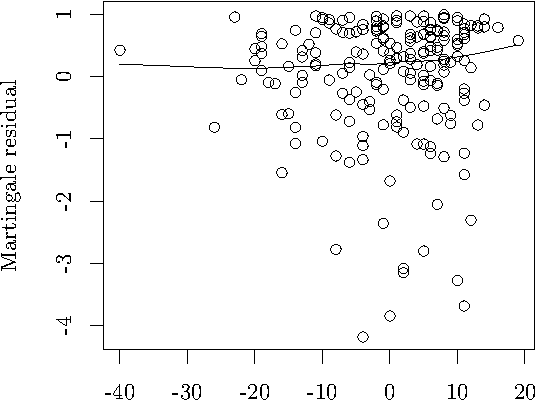
\includegraphics[width=\maxwidth]{figure/05-eda-func-form-age-1} 

}


\begin{kframe}\begin{alltt}
\hlkwd{scatter.smooth}\hlstd{(data}\hlopt{$}\hlstd{AgeCent,} \hlkwd{resid}\hlstd{(fit.cph.NoAge,} \hlkwc{type} \hlstd{=} \hlstr{"martingale"}\hlstd{),} \hlkwc{xlab} \hlstd{=} \hlstr{""}\hlstd{,} \hlkwc{ylab} \hlstd{=} \hlstr{"Martingale residual"}\hlstd{,} \hlkwc{ylim} \hlstd{=} \hlkwd{c}\hlstd{(}\hlopt{-}\hlnum{1}\hlstd{,} \hlnum{1}\hlstd{))}
\end{alltt}
\end{kframe}

{\centering 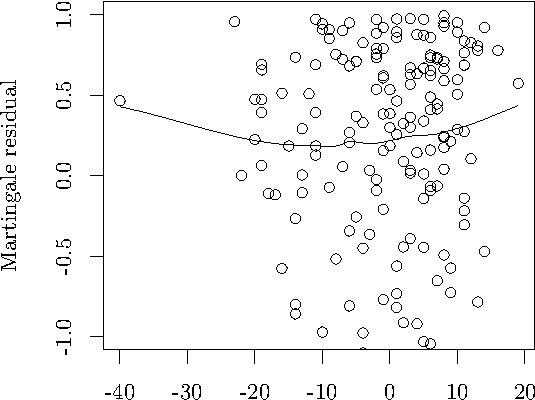
\includegraphics[width=\maxwidth]{figure/05-eda-func-form-age-2} 

}



\end{knitrout}

\begin{knitrout}
\definecolor{shadecolor}{rgb}{0.969, 0.969, 0.969}\color{fgcolor}\begin{kframe}
\begin{alltt}
\hlstd{fit.cph.NoSize} \hlkwb{=} \hlkwd{coxph}\hlstd{(}\hlkwd{Surv}\hlstd{(Time, DSD)} \hlopt{~} \hlstd{SexM} \hlopt{+} \hlstd{AgeCent} \hlopt{+} \hlstd{LocBody} \hlopt{+} \hlstd{A2} \hlopt{+} \hlstd{A4,} \hlkwc{data} \hlstd{= data)}
\hlkwd{scatter.smooth}\hlstd{(data}\hlopt{$}\hlstd{SizeCent,} \hlkwd{resid}\hlstd{(fit.cph.NoSize,} \hlkwc{type} \hlstd{=} \hlstr{"martingale"}\hlstd{),} \hlkwc{xlab} \hlstd{=} \hlstr{""}\hlstd{,} \hlkwc{ylab} \hlstd{=} \hlstr{"Martingale residual"}\hlstd{)}
\end{alltt}
\end{kframe}

{\centering 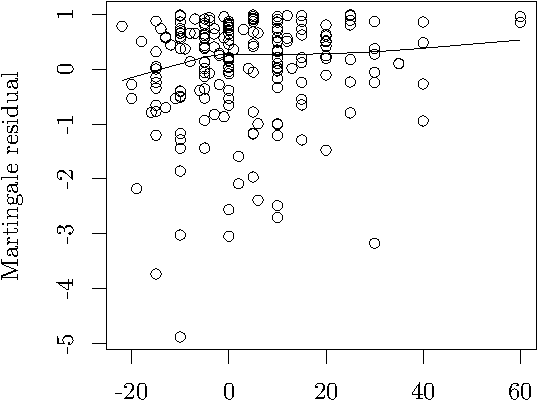
\includegraphics[width=\maxwidth]{figure/05-eda-func-form-size-1} 

}


\begin{kframe}\begin{alltt}
\hlkwd{scatter.smooth}\hlstd{(data}\hlopt{$}\hlstd{SizeCent,} \hlkwd{resid}\hlstd{(fit.cph.NoSize,} \hlkwc{type} \hlstd{=} \hlstr{"martingale"}\hlstd{),} \hlkwc{xlab} \hlstd{=} \hlstr{""}\hlstd{,} \hlkwc{ylab} \hlstd{=} \hlstr{"Martingale residual"}\hlstd{,} \hlkwc{ylim} \hlstd{=} \hlkwd{c}\hlstd{(}\hlopt{-}\hlnum{1}\hlstd{,} \hlnum{1}\hlstd{))}
\end{alltt}
\end{kframe}

{\centering 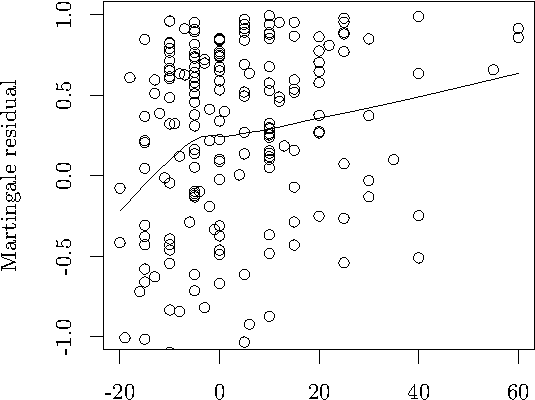
\includegraphics[width=\maxwidth]{figure/05-eda-func-form-size-2} 

}



\end{knitrout}
It looks like age has a minor nonlinear component, with a small uptick at advanced age.  Very minor though.  The size relationship appears to have a knee, close to size == 0, around which the relationship is approximately linear.

Model age as:  $AgeCent + AgeCent I(AgeCent > 0) \equiv AgeCent+ AgeCent_+$
Model size as: $SizeCent + SizeCent I(SizeCent > 0) \equiv SizeCent + SizeCent_+$

\begin{knitrout}
\definecolor{shadecolor}{rgb}{0.969, 0.969, 0.969}\color{fgcolor}\begin{kframe}
\begin{alltt}
\hlstd{data}\hlopt{$}\hlstd{AgePlus} \hlkwb{=} \hlkwd{pmax}\hlstd{(data}\hlopt{$}\hlstd{AgeCent,} \hlnum{0}\hlstd{)}
\hlstd{data}\hlopt{$}\hlstd{SizePlus} \hlkwb{=} \hlkwd{pmax}\hlstd{(data}\hlopt{$}\hlstd{SizeCent,} \hlnum{0}\hlstd{)}
\end{alltt}
\end{kframe}
\end{knitrout}


\subsection{PH assumption: full model}
\begin{knitrout}
\definecolor{shadecolor}{rgb}{0.969, 0.969, 0.969}\color{fgcolor}\begin{kframe}
\begin{alltt}
\hlstd{fit.cph} \hlkwb{=} \hlkwd{coxph}\hlstd{(}\hlkwd{Surv}\hlstd{(Time, DSD)} \hlopt{~} \hlstd{SexM} \hlopt{+} \hlstd{AgeCent} \hlopt{+} \hlstd{AgePlus} \hlopt{+} \hlstd{LocBody} \hlopt{+} \hlstd{SizeCent} \hlopt{+} \hlstd{SizePlus} \hlopt{+} \hlstd{A2} \hlopt{+} \hlstd{A4,} \hlkwc{data} \hlstd{= data)}
\hlkwd{cox.zph}\hlstd{(fit.cph)}
\end{alltt}
\begin{verbatim}
##                 rho   chisq      p
## SexMTRUE     0.1301  3.3440 0.0675
## AgeCent     -0.0399  0.3410 0.5592
## AgePlus      0.0270  0.1548 0.6940
## LocBodyTRUE -0.1008  1.8022 0.1794
## SizeCent    -0.0090  0.0148 0.9033
## SizePlus    -0.0128  0.0311 0.8600
## A2TRUE      -0.0203  0.0788 0.7790
## A4TRUE      -0.1354  3.3410 0.0676
## GLOBAL           NA 13.8497 0.0858
\end{verbatim}
\begin{alltt}
\hlkwd{plot}\hlstd{(}\hlkwd{cox.zph}\hlstd{(fit.cph)[}\hlnum{1}\hlstd{])}
\end{alltt}
\end{kframe}

{\centering 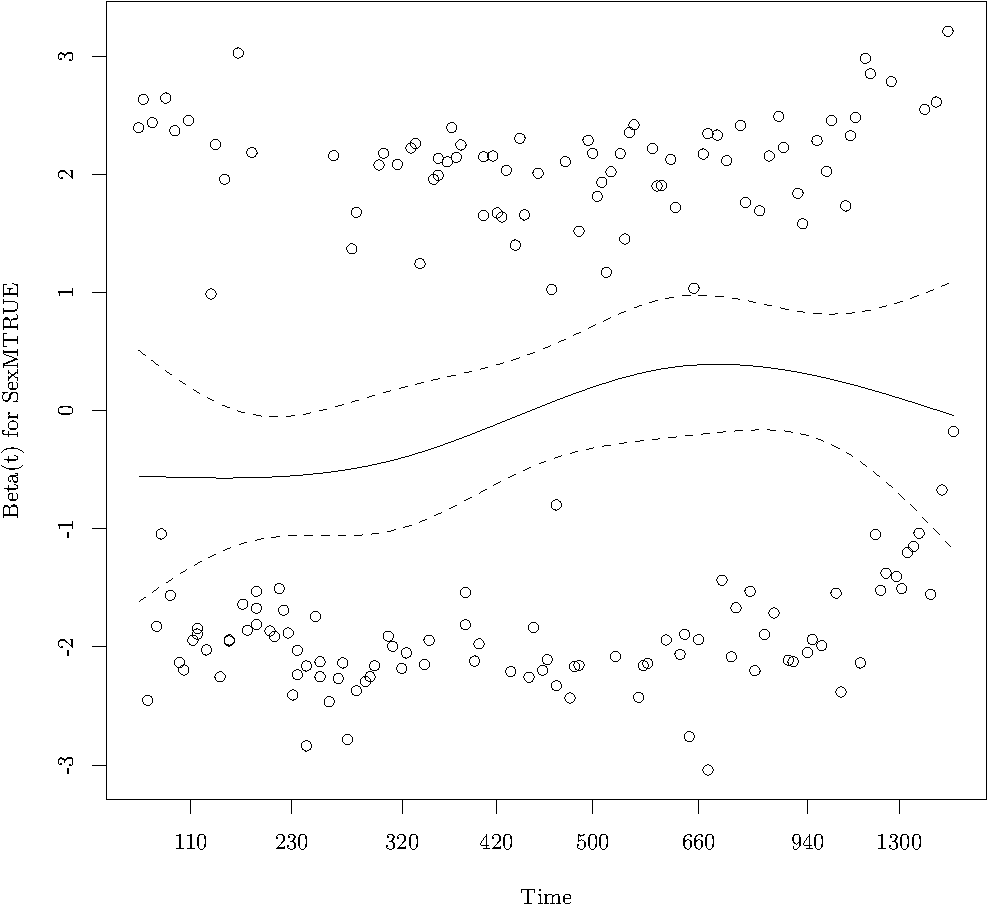
\includegraphics[width=\maxwidth]{figure/05-eda-ph-check-full-1} 

}


\begin{kframe}\begin{alltt}
\hlkwd{plot}\hlstd{(}\hlkwd{cox.zph}\hlstd{(fit.cph)[}\hlnum{8}\hlstd{])}
\end{alltt}
\end{kframe}

{\centering 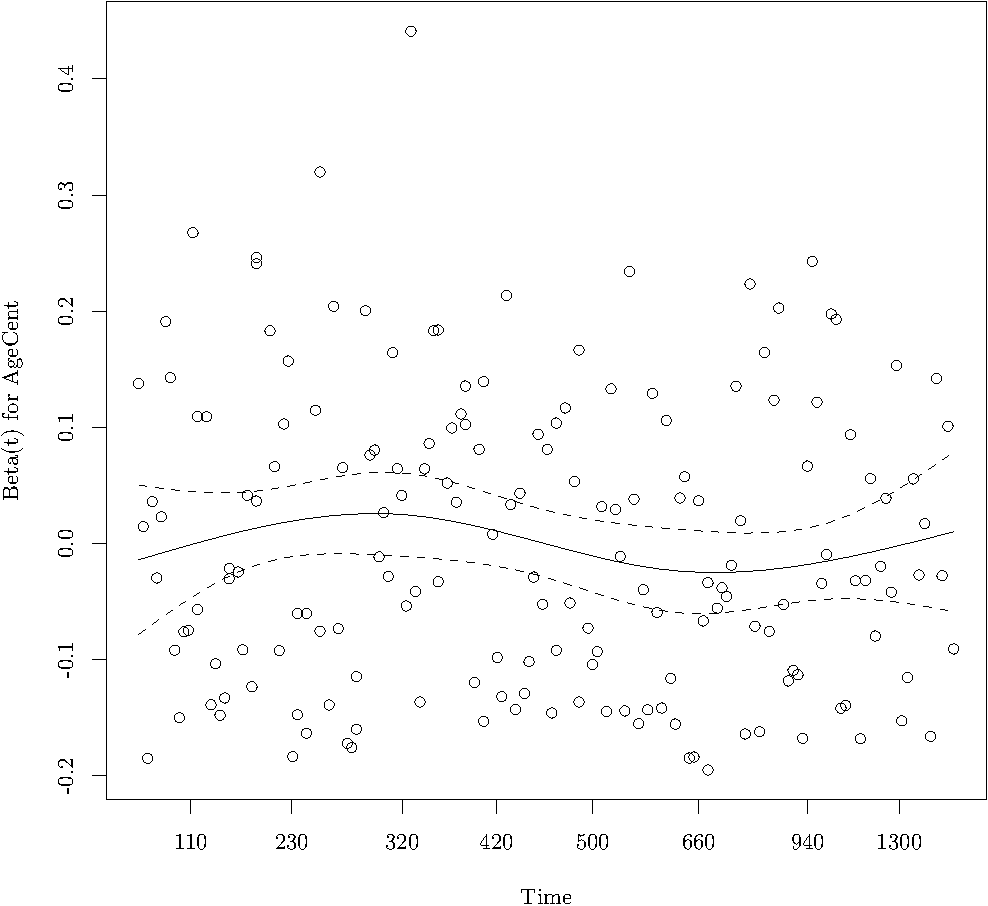
\includegraphics[width=\maxwidth]{figure/05-eda-ph-check-full-2} 

}



\end{knitrout}
Looks OK, just weak possible effects with gender and A4.


\subsection{EDA: Variable selection}
\begin{knitrout}
\definecolor{shadecolor}{rgb}{0.969, 0.969, 0.969}\color{fgcolor}\begin{kframe}
\begin{alltt}
\hlstd{nobs.coxph} \hlkwb{<<-} \hlkwa{function}\hlstd{(}\hlkwc{obj}\hlstd{,} \hlkwc{...}\hlstd{)} \hlkwd{sum}\hlstd{(obj}\hlopt{$}\hlstd{y[,}\hlnum{2}\hlstd{])}
\hlkwd{set.seed}\hlstd{(}\hlnum{20150201}\hlstd{)}
\hlstd{fit.cph.as.bic} \hlkwb{=} \hlkwd{glmulti}\hlstd{(}\hlkwd{Surv}\hlstd{(Time, DSD)} \hlopt{~} \hlstd{SexM} \hlopt{+} \hlstd{AgeCent} \hlopt{+} \hlstd{AgePlus} \hlopt{+} \hlstd{LocBody} \hlopt{+} \hlstd{SizeCent} \hlopt{+} \hlstd{SizePlus} \hlopt{+} \hlstd{A2} \hlopt{+} \hlstd{A4,} \hlkwc{data} \hlstd{= data,} \hlkwc{marginality} \hlstd{=} \hlnum{TRUE}\hlstd{,} \hlkwc{method} \hlstd{=} \hlstr{"g"}\hlstd{,} \hlkwc{fitfunction} \hlstd{=} \hlstr{"coxph"}\hlstd{,} \hlkwc{crit} \hlstd{=} \hlstr{"bic"}\hlstd{,} \hlkwc{level} \hlstd{=} \hlnum{2}\hlstd{,} \hlkwc{plotty} \hlstd{=} \hlnum{FALSE}\hlstd{,} \hlkwc{report} \hlstd{=} \hlnum{TRUE}\hlstd{)}
\end{alltt}
\begin{verbatim}
## Initialization...
## TASK: Genetic algorithm in the candidate set.
## Initialization...
## Algorithm started...
## 
## After 10 generations:
## Best model: Surv(Time,DSD)~1+SexM+AgePlus+LocBody+SizeCent+SizePlus+A2+AgePlus:SexM+LocBody:AgePlus+SizePlus:SexM+SizePlus:LocBody+A2:AgePlus+A2:SizeCent+A2:SizePlus
## Crit= 1729.11398668955
## Mean crit= 1766.92050825977
## Change in best IC: -8270.88601331045 / Change in mean IC: -8233.07949174023
\end{verbatim}


{\ttfamily\noindent\color{warningcolor}{\#\# Warning in fitter(X, Y, strats, offset, init, control, weights = weights, : Loglik converged before variable\ \ 14 ; beta may be infinite.}}\begin{verbatim}
## 
## After 20 generations:
## Best model: Surv(Time,DSD)~1+SexM+AgePlus+LocBody+SizeCent+SizePlus+A2+AgePlus:SexM+SizePlus:SexM+A2:SizeCent+A2:SizePlus
## Crit= 1713.89677467987
## Mean crit= 1762.03513325276
## Change in best IC: -15.2172120096811 / Change in mean IC: -4.88537500701909
## 
## After 30 generations:
## Best model: Surv(Time,DSD)~1+SexM+AgePlus+LocBody+SizeCent+SizePlus+A2+A4+AgePlus:SexM+SizePlus:SexM+A2:SizeCent+A2:SizePlus
## Crit= 1713.29309640268
## Mean crit= 1757.77883565899
## Change in best IC: -0.603678277190284 / Change in mean IC: -4.25629759376807
\end{verbatim}


{\ttfamily\noindent\color{warningcolor}{\#\# Warning in fitter(X, Y, strats, offset, init, control, weights = weights, : Loglik converged before variable\ \ 4 ; beta may be infinite.}}\begin{verbatim}
## 
## After 40 generations:
## Best model: Surv(Time,DSD)~1+SexM+AgePlus+SizeCent+SizePlus+A2+A4+AgePlus:SexM+SizePlus:SexM+A2:SizeCent+A2:SizePlus
## Crit= 1709.60872011004
## Mean crit= 1754.83822914144
## Change in best IC: -3.68437629263758 / Change in mean IC: -2.9406065175499
\end{verbatim}


{\ttfamily\noindent\color{warningcolor}{\#\# Warning in fitter(X, Y, strats, offset, init, control, weights = weights, : Loglik converged before variable\ \ 3 ; beta may be infinite.}}\begin{verbatim}
## 
## After 50 generations:
## Best model: Surv(Time,DSD)~1+SexM+SizeCent+SizePlus+A2+A4+SizePlus:SexM+A2:SizeCent+A2:SizePlus
## Crit= 1702.15368169776
## Mean crit= 1751.82996915762
## Change in best IC: -7.45503841228765 / Change in mean IC: -3.00825998381674
## 
## After 60 generations:
## Best model: Surv(Time,DSD)~1+SexM+SizeCent+SizePlus+A2+A4+SizePlus:SexM+A2:SizeCent+A2:SizePlus
## Crit= 1702.15368169776
## Mean crit= 1749.23525857307
## Change in best IC: 0 / Change in mean IC: -2.59471058455279
## 
## After 70 generations:
## Best model: Surv(Time,DSD)~1+SexM+SizeCent+SizePlus+A2+A4+SizePlus:SexM+A2:SizeCent+A2:SizePlus
## Crit= 1702.15368169776
## Mean crit= 1748.18423062138
## Change in best IC: 0 / Change in mean IC: -1.05102795169159
## 
## After 80 generations:
## Best model: Surv(Time,DSD)~1+SexM+SizeCent+SizePlus+A2+A4+A2:SizeCent+A2:SizePlus
## Crit= 1700.85916505495
## Mean crit= 1745.87214391533
## Change in best IC: -1.29451664280623 / Change in mean IC: -2.31208670604769
## 
## After 90 generations:
## Best model: Surv(Time,DSD)~1+SexM+SizeCent+SizePlus+A2+A4+A2:SizeCent+A2:SizePlus
## Crit= 1700.85916505495
## Mean crit= 1743.80961114713
## Change in best IC: 0 / Change in mean IC: -2.06253276820053
## 
## After 100 generations:
## Best model: Surv(Time,DSD)~1+SizePlus+A2+A4
## Crit= 1687.23535748033
## Mean crit= 1741.17763508212
## Change in best IC: -13.6238075746228 / Change in mean IC: -2.63197606500398
## 
## After 110 generations:
## Best model: Surv(Time,DSD)~1+SizePlus+A2+A4
## Crit= 1687.23535748033
## Mean crit= 1740.57831818846
## Change in best IC: 0 / Change in mean IC: -0.599316893664536
## 
## After 120 generations:
## Best model: Surv(Time,DSD)~1+SizePlus+A2+A4
## Crit= 1687.23535748033
## Mean crit= 1738.63857426502
## Change in best IC: 0 / Change in mean IC: -1.93974392344398
## 
## After 130 generations:
## Best model: Surv(Time,DSD)~1+SizePlus+A2+A4
## Crit= 1687.23535748033
## Mean crit= 1737.42400630752
## Change in best IC: 0 / Change in mean IC: -1.21456795749828
## 
## After 140 generations:
## Best model: Surv(Time,DSD)~1+SizePlus+A2+A4
## Crit= 1687.23535748033
## Mean crit= 1737.12117927695
## Change in best IC: 0 / Change in mean IC: -0.302827030562639
## 
## After 150 generations:
## Best model: Surv(Time,DSD)~1+SizePlus+A2+A4
## Crit= 1687.23535748033
## Mean crit= 1735.68266270197
## Change in best IC: 0 / Change in mean IC: -1.43851657498431
## 
## After 160 generations:
## Best model: Surv(Time,DSD)~1+SizePlus+A2+A4
## Crit= 1687.23535748033
## Mean crit= 1735.31128667725
## Change in best IC: 0 / Change in mean IC: -0.371376024724441
## 
## After 170 generations:
## Best model: Surv(Time,DSD)~1+SizePlus+A2+A4
## Crit= 1687.23535748033
## Mean crit= 1734.60899780354
## Change in best IC: 0 / Change in mean IC: -0.702288873701718
\end{verbatim}


{\ttfamily\noindent\color{warningcolor}{\#\# Warning in fitter(X, Y, strats, offset, init, control, weights = weights, : Loglik converged before variable\ \ 4 ; beta may be infinite.}}\begin{verbatim}
## 
## After 180 generations:
## Best model: Surv(Time,DSD)~1+SizePlus+A2+A4
## Crit= 1687.23535748033
## Mean crit= 1734.41964369079
## Change in best IC: 0 / Change in mean IC: -0.189354112751971
## 
## After 190 generations:
## Best model: Surv(Time,DSD)~1+SizePlus+A2+A4
## Crit= 1687.23535748033
## Mean crit= 1733.36722791485
## Change in best IC: 0 / Change in mean IC: -1.05241577594325
## 
## After 200 generations:
## Best model: Surv(Time,DSD)~1+SizePlus+A2+A4
## Crit= 1687.23535748033
## Mean crit= 1733.19680151486
## Change in best IC: 0 / Change in mean IC: -0.170426399986354
\end{verbatim}


{\ttfamily\noindent\color{warningcolor}{\#\# Warning in fitter(X, Y, strats, offset, init, control, weights = weights, : Loglik converged before variable\ \ 1 ; beta may be infinite.}}\begin{verbatim}
## 
## After 210 generations:
## Best model: Surv(Time,DSD)~1+SizePlus+A2+A4
## Crit= 1687.23535748033
## Mean crit= 1732.96389151369
## Change in best IC: 0 / Change in mean IC: -0.232910001176151
## 
## After 220 generations:
## Best model: Surv(Time,DSD)~1+SizePlus+A2+A4
## Crit= 1687.23535748033
## Mean crit= 1732.11325171291
## Change in best IC: 0 / Change in mean IC: -0.850639800774161
## 
## After 230 generations:
## Best model: Surv(Time,DSD)~1+SizePlus+A2+A4
## Crit= 1687.23535748033
## Mean crit= 1731.87559655747
## Change in best IC: 0 / Change in mean IC: -0.237655155437551
## 
## After 240 generations:
## Best model: Surv(Time,DSD)~1+SizePlus+A2+A4
## Crit= 1687.23535748033
## Mean crit= 1731.61898120716
## Change in best IC: 0 / Change in mean IC: -0.256615350314632
## 
## After 250 generations:
## Best model: Surv(Time,DSD)~1+SizePlus+A2+A4
## Crit= 1687.23535748033
## Mean crit= 1731.30594054392
## Change in best IC: 0 / Change in mean IC: -0.313040663238098
## 
## After 260 generations:
## Best model: Surv(Time,DSD)~1+SizePlus+A2+A4
## Crit= 1687.23535748033
## Mean crit= 1730.31673935724
## Change in best IC: 0 / Change in mean IC: -0.98920118668434
## 
## After 270 generations:
## Best model: Surv(Time,DSD)~1+SizePlus+A2+A4
## Crit= 1687.23535748033
## Mean crit= 1730.31673935724
## Change in best IC: 0 / Change in mean IC: 0
## 
## After 280 generations:
## Best model: Surv(Time,DSD)~1+SizePlus+A2+A4
## Crit= 1687.23535748033
## Mean crit= 1730.31382715624
## Change in best IC: 0 / Change in mean IC: -0.00291220100166356
## 
## After 290 generations:
## Best model: Surv(Time,DSD)~1+SizePlus+A2+A4
## Crit= 1687.23535748033
## Mean crit= 1729.85554785647
## Change in best IC: 0 / Change in mean IC: -0.458279299763944
## 
## After 300 generations:
## Best model: Surv(Time,DSD)~1+SizePlus+A2+A4
## Crit= 1687.23535748033
## Mean crit= 1729.77539491139
## Change in best IC: 0 / Change in mean IC: -0.0801529450802718
## 
## After 310 generations:
## Best model: Surv(Time,DSD)~1+SizePlus+A2+A4
## Crit= 1687.23535748033
## Mean crit= 1729.71168475816
## Change in best IC: 0 / Change in mean IC: -0.063710153233842
## 
## After 320 generations:
## Best model: Surv(Time,DSD)~1+SizePlus+A2+A4
## Crit= 1687.23535748033
## Mean crit= 1729.09784964428
## Change in best IC: 0 / Change in mean IC: -0.613835113879759
## 
## After 330 generations:
## Best model: Surv(Time,DSD)~1+SizePlus+A2+A4
## Crit= 1687.23535748033
## Mean crit= 1729.08455299787
## Change in best IC: 0 / Change in mean IC: -0.0132966464104811
\end{verbatim}


{\ttfamily\noindent\color{warningcolor}{\#\# Warning in fitter(X, Y, strats, offset, init, control, weights = weights, : Loglik converged before variable\ \ 17 ; beta may be infinite.}}\begin{verbatim}
## 
## After 340 generations:
## Best model: Surv(Time,DSD)~1+SizePlus+A2+A4
## Crit= 1687.23535748033
## Mean crit= 1728.9937020156
## Change in best IC: 0 / Change in mean IC: -0.0908509822693304
## 
## After 350 generations:
## Best model: Surv(Time,DSD)~1+SizePlus+A2+A4
## Crit= 1687.23535748033
## Mean crit= 1728.9381191167
## Change in best IC: 0 / Change in mean IC: -0.0555828989029123
## 
## After 360 generations:
## Best model: Surv(Time,DSD)~1+SizePlus+A2+A4
## Crit= 1687.23535748033
## Mean crit= 1728.28650181196
## Change in best IC: 0 / Change in mean IC: -0.651617304730735
## 
## After 370 generations:
## Best model: Surv(Time,DSD)~1+SizePlus+A2+A4
## Crit= 1687.23535748033
## Mean crit= 1728.1371550272
## Change in best IC: 0 / Change in mean IC: -0.149346784767204
## 
## After 380 generations:
## Best model: Surv(Time,DSD)~1+SizePlus+A2+A4
## Crit= 1687.23535748033
## Mean crit= 1728.05668123256
## Change in best IC: 0 / Change in mean IC: -0.0804737946371006
## 
## After 390 generations:
## Best model: Surv(Time,DSD)~1+SizePlus+A2+A4
## Crit= 1687.23535748033
## Mean crit= 1728.05668123256
## Change in best IC: 0 / Change in mean IC: 0
## 
## After 400 generations:
## Best model: Surv(Time,DSD)~1+SizePlus+A2+A4
## Crit= 1687.23535748033
## Mean crit= 1728.05668123256
## Change in best IC: 0 / Change in mean IC: 0
## 
## After 410 generations:
## Best model: Surv(Time,DSD)~1+SizePlus+A2+A4
## Crit= 1687.23535748033
## Mean crit= 1727.90861153151
## Change in best IC: 0 / Change in mean IC: -0.148069701052691
## 
## After 420 generations:
## Best model: Surv(Time,DSD)~1+SizePlus+A2+A4
## Crit= 1687.23535748033
## Mean crit= 1727.65672333188
## Change in best IC: 0 / Change in mean IC: -0.251888199624773
## 
## After 430 generations:
## Best model: Surv(Time,DSD)~1+SizePlus+A2+A4
## Crit= 1687.23535748033
## Mean crit= 1727.42475825227
## Change in best IC: 0 / Change in mean IC: -0.23196507961643
## 
## After 440 generations:
## Best model: Surv(Time,DSD)~1+SizePlus+A2+A4
## Crit= 1687.23535748033
## Mean crit= 1727.37968944642
## Change in best IC: 0 / Change in mean IC: -0.0450688058429023
## 
## After 450 generations:
## Best model: Surv(Time,DSD)~1+SizePlus+A2+A4
## Crit= 1687.23535748033
## Mean crit= 1727.37968944642
## Change in best IC: 0 / Change in mean IC: 0
## 
## After 460 generations:
## Best model: Surv(Time,DSD)~1+SizePlus+A2+A4
## Crit= 1687.23535748033
## Mean crit= 1727.25440946714
## Change in best IC: 0 / Change in mean IC: -0.125279979287598
## 
## After 470 generations:
## Best model: Surv(Time,DSD)~1+SizePlus+A2+A4
## Crit= 1687.23535748033
## Mean crit= 1727.08037862017
## Change in best IC: 0 / Change in mean IC: -0.174030846962523
## 
## After 480 generations:
## Best model: Surv(Time,DSD)~1+SizePlus+A2+A4
## Crit= 1687.23535748033
## Mean crit= 1726.91678585524
## Change in best IC: 0 / Change in mean IC: -0.163592764933583
## 
## After 490 generations:
## Best model: Surv(Time,DSD)~1+SizePlus+A2+A4
## Crit= 1687.23535748033
## Mean crit= 1726.86709407315
## Change in best IC: 0 / Change in mean IC: -0.0496917820873932
## 
## After 500 generations:
## Best model: Surv(Time,DSD)~1+SizePlus+A2+A4
## Crit= 1687.23535748033
## Mean crit= 1726.8122935298
## Change in best IC: 0 / Change in mean IC: -0.0548005433477101
## 
## After 510 generations:
## Best model: Surv(Time,DSD)~1+SizePlus+A2+A4
## Crit= 1687.23535748033
## Mean crit= 1726.77802944676
## Change in best IC: 0 / Change in mean IC: -0.0342640830460823
## 
## After 520 generations:
## Best model: Surv(Time,DSD)~1+SizePlus+A2+A4
## Crit= 1687.23535748033
## Mean crit= 1726.26274628995
## Change in best IC: 0 / Change in mean IC: -0.515283156804799
## 
## After 530 generations:
## Best model: Surv(Time,DSD)~1+SizePlus+A2+A4
## Crit= 1687.23535748033
## Mean crit= 1726.24361440849
## Change in best IC: 0 / Change in mean IC: -0.0191318814613624
## 
## After 540 generations:
## Best model: Surv(Time,DSD)~1+SizePlus+A2+A4
## Crit= 1687.23535748033
## Mean crit= 1726.09238620418
## Change in best IC: 0 / Change in mean IC: -0.151228204315885
## 
## After 550 generations:
## Best model: Surv(Time,DSD)~1+SizePlus+A2+A4
## Crit= 1687.23535748033
## Mean crit= 1726.09238620418
## Change in best IC: 0 / Change in mean IC: 0
## 
## After 560 generations:
## Best model: Surv(Time,DSD)~1+SizePlus+A2+A4
## Crit= 1687.23535748033
## Mean crit= 1726.09238620418
## Change in best IC: 0 / Change in mean IC: 0
## 
## After 570 generations:
## Best model: Surv(Time,DSD)~1+SizePlus+A2+A4
## Crit= 1687.23535748033
## Mean crit= 1726.06627923278
## Change in best IC: 0 / Change in mean IC: -0.026106971393574
## 
## After 580 generations:
## Best model: Surv(Time,DSD)~1+SizePlus+A2+A4
## Crit= 1687.23535748033
## Mean crit= 1726.06627923278
## Change in best IC: 0 / Change in mean IC: 0
## 
## After 590 generations:
## Best model: Surv(Time,DSD)~1+SizePlus+A2+A4
## Crit= 1687.23535748033
## Mean crit= 1726.06627923278
## Improvements in best and average IC have bebingo en below the specified goals.
## Algorithm is declared to have converged.
## Completed.
\end{verbatim}
\begin{alltt}
\hlstd{fit.cph.as.aicc} \hlkwb{=} \hlkwd{glmulti}\hlstd{(}\hlkwd{Surv}\hlstd{(Time, DSD)} \hlopt{~} \hlstd{SexM} \hlopt{+} \hlstd{AgeCent} \hlopt{+} \hlstd{AgePlus} \hlopt{+} \hlstd{LocBody} \hlopt{+} \hlstd{SizeCent} \hlopt{+} \hlstd{SizePlus} \hlopt{+} \hlstd{A2} \hlopt{+} \hlstd{A4,} \hlkwc{data} \hlstd{= data,} \hlkwc{marginality} \hlstd{=} \hlnum{TRUE}\hlstd{,} \hlkwc{method} \hlstd{=} \hlstr{"g"}\hlstd{,} \hlkwc{fitfunction} \hlstd{=} \hlstr{"coxph"}\hlstd{,} \hlkwc{crit} \hlstd{=} \hlstr{"aicc"}\hlstd{,} \hlkwc{level} \hlstd{=} \hlnum{2}\hlstd{,} \hlkwc{plotty} \hlstd{=} \hlnum{FALSE}\hlstd{,} \hlkwc{report} \hlstd{=} \hlnum{TRUE}\hlstd{)}
\end{alltt}
\begin{verbatim}
## Initialization...
## TASK: Genetic algorithm in the candidate set.
## Initialization...
## Algorithm started...
\end{verbatim}


{\ttfamily\noindent\color{warningcolor}{\#\# Warning in fitter(X, Y, strats, offset, init, control, weights = weights, : Loglik converged before variable\ \ 6 ; beta may be infinite.}}\begin{verbatim}
## 
## After 10 generations:
## Best model: Surv(Time,DSD)~1+SexM+LocBody+SizeCent+SizePlus+A2+A4+LocBody:SexM+A2:SizeCent+A2:SizePlus+A4:SizeCent
## Crit= 1682.0367331261
## Mean crit= 1701.43959331731
## Change in best IC: -8317.9632668739 / Change in mean IC: -8298.56040668269
## 
## After 20 generations:
## Best model: Surv(Time,DSD)~1+SexM+LocBody+SizeCent+SizePlus+A2+A4+LocBody:SexM+SizePlus:SexM+A2:SizeCent+A2:SizePlus+A4:SizeCent
## Crit= 1680.97132981957
## Mean crit= 1698.17607519783
## Change in best IC: -1.06540330652274 / Change in mean IC: -3.2635181194878
## 
## After 30 generations:
## Best model: Surv(Time,DSD)~1+SexM+SizeCent+SizePlus+A2+A4+SizeCent:SexM+A2:SizeCent+A2:SizePlus+A4:SizeCent
## Crit= 1678.76908814612
## Mean crit= 1696.58275412683
## Change in best IC: -2.202241673456 / Change in mean IC: -1.59332107099658
## 
## After 40 generations:
## Best model: Surv(Time,DSD)~1+SizeCent+SizePlus+A2+A4+A2:SizeCent+A2:SizePlus+A4:SizeCent+A4:A2
## Crit= 1675.76250594588
## Mean crit= 1695.27966728063
## Change in best IC: -3.00658220023797 / Change in mean IC: -1.30308684619945
## 
## After 50 generations:
## Best model: Surv(Time,DSD)~1+SizeCent+SizePlus+A2+A4+A2:SizeCent+A2:SizePlus+A4:SizeCent+A4:A2
## Crit= 1675.76250594588
## Mean crit= 1694.44562102112
## Change in best IC: 0 / Change in mean IC: -0.834046259508341
## 
## After 60 generations:
## Best model: Surv(Time,DSD)~1+SizeCent+SizePlus+A2+A4+A2:SizeCent+A2:SizePlus+A4:SizeCent+A4:A2
## Crit= 1675.76250594588
## Mean crit= 1693.66057977912
## Change in best IC: 0 / Change in mean IC: -0.785041242000716
## 
## After 70 generations:
## Best model: Surv(Time,DSD)~1+SizeCent+SizePlus+A2+A4+A2:SizeCent+A2:SizePlus+A4:SizeCent+A4:A2
## Crit= 1675.76250594588
## Mean crit= 1693.30593845584
## Change in best IC: 0 / Change in mean IC: -0.354641323285932
## 
## After 80 generations:
## Best model: Surv(Time,DSD)~1+SizeCent+SizePlus+A2+A4+A2:SizeCent+A2:SizePlus+A4:SizeCent+A4:A2
## Crit= 1675.76250594588
## Mean crit= 1693.00346534139
## Change in best IC: 0 / Change in mean IC: -0.302473114443956
\end{verbatim}


{\ttfamily\noindent\color{warningcolor}{\#\# Warning in fitter(X, Y, strats, offset, init, control, weights = weights, : Loglik converged before variable\ \ 13 ; beta may be infinite.}}\begin{verbatim}
## 
## After 90 generations:
## Best model: Surv(Time,DSD)~1+SizeCent+SizePlus+A2+A4+A2:SizeCent+A2:SizePlus+A4:SizeCent+A4:A2
## Crit= 1675.76250594588
## Mean crit= 1692.46250272724
## Change in best IC: 0 / Change in mean IC: -0.540962614148157
## 
## After 100 generations:
## Best model: Surv(Time,DSD)~1+SizeCent+SizePlus+A2+A4+A2:SizeCent+A2:SizePlus+A4:SizeCent+A4:A2
## Crit= 1675.76250594588
## Mean crit= 1692.16052441245
## Change in best IC: 0 / Change in mean IC: -0.301978314797452
## 
## After 110 generations:
## Best model: Surv(Time,DSD)~1+SizeCent+SizePlus+A2+A4+A2:SizeCent+A2:SizePlus+A4:SizeCent+A4:A2
## Crit= 1675.76250594588
## Mean crit= 1691.94450362254
## Change in best IC: 0 / Change in mean IC: -0.216020789902814
## 
## After 120 generations:
## Best model: Surv(Time,DSD)~1+SizeCent+SizePlus+A2+A4+A2:SizeCent+A2:SizePlus+A4:SizeCent+A4:A2
## Crit= 1675.76250594588
## Mean crit= 1691.71900201189
## Change in best IC: 0 / Change in mean IC: -0.225501610656238
## 
## After 130 generations:
## Best model: Surv(Time,DSD)~1+SizeCent+SizePlus+A2+A4+A2:SizeCent+A2:SizePlus+A4:SizeCent+A4:A2
## Crit= 1675.76250594588
## Mean crit= 1691.55647166699
## Change in best IC: 0 / Change in mean IC: -0.162530344895686
## 
## After 140 generations:
## Best model: Surv(Time,DSD)~1+SizeCent+SizePlus+A2+A4+A2:SizeCent+A2:SizePlus+A4:SizeCent+A4:A2
## Crit= 1675.76250594588
## Mean crit= 1691.54947337523
## Change in best IC: 0 / Change in mean IC: -0.00699829176596722
## 
## After 150 generations:
## Best model: Surv(Time,DSD)~1+SizeCent+SizePlus+A2+A4+A2:SizeCent+A2:SizePlus+A4:A2
## Crit= 1675.67251928033
## Mean crit= 1691.20002595634
## Change in best IC: -0.0899866655549886 / Change in mean IC: -0.349447418882619
## 
## After 160 generations:
## Best model: Surv(Time,DSD)~1+SizeCent+SizePlus+A2+A4+A2:SizeCent+A2:SizePlus+A4:A2
## Crit= 1675.67251928033
## Mean crit= 1691.14269036956
## Change in best IC: 0 / Change in mean IC: -0.0573355867809369
## 
## After 170 generations:
## Best model: Surv(Time,DSD)~1+SizeCent+SizePlus+A2+A4+A2:SizeCent+A2:SizePlus+A4:A2
## Crit= 1675.67251928033
## Mean crit= 1691.00186336932
## Change in best IC: 0 / Change in mean IC: -0.140827000242098
## 
## After 180 generations:
## Best model: Surv(Time,DSD)~1+SizeCent+SizePlus+A2+A4+A2:SizeCent+A2:SizePlus+A4:A2
## Crit= 1675.67251928033
## Mean crit= 1690.73836137131
## Change in best IC: 0 / Change in mean IC: -0.263501998009588
## 
## After 190 generations:
## Best model: Surv(Time,DSD)~1+SizeCent+SizePlus+A2+A4+A2:SizeCent+A2:SizePlus+A4:A2
## Crit= 1675.67251928033
## Mean crit= 1690.50196968902
## Change in best IC: 0 / Change in mean IC: -0.236391682293061
## 
## After 200 generations:
## Best model: Surv(Time,DSD)~1+SizeCent+SizePlus+A2+A4+A2:SizeCent+A2:SizePlus+A4:A2
## Crit= 1675.67251928033
## Mean crit= 1690.37291838075
## Change in best IC: 0 / Change in mean IC: -0.129051308264025
## 
## After 210 generations:
## Best model: Surv(Time,DSD)~1+SizeCent+SizePlus+A2+A4+A2:SizeCent+A2:SizePlus+A4:A2
## Crit= 1675.67251928033
## Mean crit= 1690.14564967821
## Change in best IC: 0 / Change in mean IC: -0.227268702542915
## 
## After 220 generations:
## Best model: Surv(Time,DSD)~1+SizeCent+SizePlus+A2+A4+A2:SizeCent+A2:SizePlus+A4:A2
## Crit= 1675.67251928033
## Mean crit= 1689.89402162152
## Change in best IC: 0 / Change in mean IC: -0.251628056689697
## 
## After 230 generations:
## Best model: Surv(Time,DSD)~1+SizeCent+SizePlus+A2+A4+A2:SizeCent+A2:SizePlus+A4:A2
## Crit= 1675.67251928033
## Mean crit= 1689.53899517239
## Change in best IC: 0 / Change in mean IC: -0.35502644913322
## 
## After 240 generations:
## Best model: Surv(Time,DSD)~1+SizeCent+SizePlus+A2+A4+A2:SizeCent+A2:SizePlus+A4:A2
## Crit= 1675.67251928033
## Mean crit= 1689.40135809754
## Change in best IC: 0 / Change in mean IC: -0.137637074846907
## 
## After 250 generations:
## Best model: Surv(Time,DSD)~1+SizeCent+SizePlus+A2+A4+A2:SizeCent+A2:SizePlus+A4:SizePlus+A4:A2
## Crit= 1675.01837714277
## Mean crit= 1689.00722341922
## Change in best IC: -0.654142137557301 / Change in mean IC: -0.394134678323326
\end{verbatim}


{\ttfamily\noindent\color{warningcolor}{\#\# Warning in fitter(X, Y, strats, offset, init, control, weights = weights, : Loglik converged before variable\ \ 17 ; beta may be infinite.}}\begin{verbatim}
## 
## After 260 generations:
## Best model: Surv(Time,DSD)~1+SizeCent+SizePlus+A2+A4+A2:SizeCent+A2:SizePlus+A4:SizePlus+A4:A2
## Crit= 1675.01837714277
## Mean crit= 1688.95626024994
## Change in best IC: 0 / Change in mean IC: -0.0509631692809762
## 
## After 270 generations:
## Best model: Surv(Time,DSD)~1+SizeCent+SizePlus+A2+A4+A2:SizeCent+A2:SizePlus+A4:SizePlus+A4:A2
## Crit= 1675.01837714277
## Mean crit= 1688.95626024994
## Change in best IC: 0 / Change in mean IC: 0
## 
## After 280 generations:
## Best model: Surv(Time,DSD)~1+SizeCent+SizePlus+A2+A4+A2:SizeCent+A2:SizePlus+A4:SizePlus+A4:A2
## Crit= 1675.01837714277
## Mean crit= 1688.72623331464
## Change in best IC: 0 / Change in mean IC: -0.230026935291335
## 
## After 290 generations:
## Best model: Surv(Time,DSD)~1+SizeCent+SizePlus+A2+A4+A2:SizeCent+A2:SizePlus+A4:SizePlus+A4:A2
## Crit= 1675.01837714277
## Mean crit= 1688.5133035274
## Change in best IC: 0 / Change in mean IC: -0.212929787243411
\end{verbatim}


{\ttfamily\noindent\color{warningcolor}{\#\# Warning in fitter(X, Y, strats, offset, init, control, weights = weights, : Loglik converged before variable\ \ 4 ; beta may be infinite.}}

{\ttfamily\noindent\color{warningcolor}{\#\# Warning in fitter(X, Y, strats, offset, init, control, weights = weights, : Loglik converged before variable\ \ 11 ; beta may be infinite.}}\begin{verbatim}
## 
## After 300 generations:
## Best model: Surv(Time,DSD)~1+SizeCent+SizePlus+A2+A4+A2:SizeCent+A2:SizePlus+A4:SizePlus+A4:A2
## Crit= 1675.01837714277
## Mean crit= 1688.35219417578
## Change in best IC: 0 / Change in mean IC: -0.161109351620553
## 
## After 310 generations:
## Best model: Surv(Time,DSD)~1+SizeCent+SizePlus+A2+A4+A2:SizeCent+A2:SizePlus+A4:SizePlus+A4:A2
## Crit= 1675.01837714277
## Mean crit= 1687.95337990679
## Change in best IC: 0 / Change in mean IC: -0.398814268989781
## 
## After 320 generations:
## Best model: Surv(Time,DSD)~1+SizeCent+SizePlus+A2+A4+A2:SizeCent+A2:SizePlus+A4:SizePlus+A4:A2
## Crit= 1675.01837714277
## Mean crit= 1687.69542765853
## Change in best IC: 0 / Change in mean IC: -0.257952248265383
## 
## After 330 generations:
## Best model: Surv(Time,DSD)~1+SizeCent+SizePlus+A2+A4+A2:SizeCent+A2:SizePlus+A4:SizePlus+A4:A2
## Crit= 1675.01837714277
## Mean crit= 1687.64425283983
## Change in best IC: 0 / Change in mean IC: -0.0511748187000194
## 
## After 340 generations:
## Best model: Surv(Time,DSD)~1+SizeCent+SizePlus+A2+A4+A2:SizeCent+A2:SizePlus+A4:SizePlus+A4:A2
## Crit= 1675.01837714277
## Mean crit= 1687.59517301127
## Change in best IC: 0 / Change in mean IC: -0.0490798285557048
## 
## After 350 generations:
## Best model: Surv(Time,DSD)~1+SizeCent+SizePlus+A2+A4+A2:SizeCent+A2:SizePlus+A4:SizePlus+A4:A2
## Crit= 1675.01837714277
## Mean crit= 1687.47004377438
## Change in best IC: 0 / Change in mean IC: -0.125129236890871
## 
## After 360 generations:
## Best model: Surv(Time,DSD)~1+SizeCent+SizePlus+A2+A4+A2:SizeCent+A2:SizePlus+A4:SizePlus+A4:A2
## Crit= 1675.01837714277
## Mean crit= 1687.2452591239
## Change in best IC: 0 / Change in mean IC: -0.224784650478796
## 
## After 370 generations:
## Best model: Surv(Time,DSD)~1+SizeCent+SizePlus+A2+A4+A2:SizeCent+A2:SizePlus+A4:SizePlus+A4:A2
## Crit= 1675.01837714277
## Mean crit= 1687.2452591239
## Change in best IC: 0 / Change in mean IC: 0
## 
## After 380 generations:
## Best model: Surv(Time,DSD)~1+SizeCent+SizePlus+A2+A4+A2:SizeCent+A2:SizePlus+A4:SizePlus+A4:A2
## Crit= 1675.01837714277
## Mean crit= 1687.06641248733
## Change in best IC: 0 / Change in mean IC: -0.178846636574235
## 
## After 390 generations:
## Best model: Surv(Time,DSD)~1+SizeCent+SizePlus+A2+A4+A2:SizeCent+A2:SizePlus+A4:SizePlus+A4:A2
## Crit= 1675.01837714277
## Mean crit= 1686.97796437564
## Change in best IC: 0 / Change in mean IC: -0.0884481116850111
## 
## After 400 generations:
## Best model: Surv(Time,DSD)~1+SizeCent+SizePlus+A2+A4+A2:SizeCent+A2:SizePlus+A4:SizePlus+A4:A2
## Crit= 1675.01837714277
## Mean crit= 1686.97796437564
## Change in best IC: 0 / Change in mean IC: 0
## 
## After 410 generations:
## Best model: Surv(Time,DSD)~1+SizeCent+SizePlus+A2+A4+A2:SizeCent+A2:SizePlus+A4:SizePlus+A4:A2
## Crit= 1675.01837714277
## Mean crit= 1686.93285703996
## Change in best IC: 0 / Change in mean IC: -0.045107335684861
## 
## After 420 generations:
## Best model: Surv(Time,DSD)~1+SizeCent+SizePlus+A2+A4+A2:SizeCent+A2:SizePlus+A4:SizePlus+A4:A2
## Crit= 1675.01837714277
## Mean crit= 1686.90184290329
## Change in best IC: 0 / Change in mean IC: -0.0310141366694552
## 
## After 430 generations:
## Best model: Surv(Time,DSD)~1+SizeCent+SizePlus+A2+A4+A2:SizeCent+A2:SizePlus+A4:SizePlus+A4:A2
## Crit= 1675.01837714277
## Mean crit= 1686.88850429184
## Change in best IC: 0 / Change in mean IC: -0.0133386114503082
## 
## After 440 generations:
## Best model: Surv(Time,DSD)~1+SizeCent+SizePlus+A2+A4+A2:SizeCent+A2:SizePlus+A4:SizePlus+A4:A2
## Crit= 1675.01837714277
## Mean crit= 1686.88850429184
## Improvements in best and average IC have bebingo en below the specified goals.
## Algorithm is declared to have converged.
## Completed.
\end{verbatim}
\begin{alltt}
\hlstd{fit.cph.as} \hlkwb{=} \hlstd{fit.cph.as.bic}
\hlkwd{rm}\hlstd{(nobs.coxph)}
\end{alltt}
\end{kframe}
\end{knitrout}

Also run BIC stepwise, because we can.
\begin{knitrout}
\definecolor{shadecolor}{rgb}{0.969, 0.969, 0.969}\color{fgcolor}\begin{kframe}
\begin{alltt}
\hlkwd{stepAIC}\hlstd{(fit.cph,} \hlkwc{k} \hlstd{=} \hlkwd{log}\hlstd{(}\hlkwd{nrow}\hlstd{(data)))}
\end{alltt}
\begin{verbatim}
## Start:  AIC=1709
## Surv(Time, DSD) ~ SexM + AgeCent + AgePlus + LocBody + SizeCent + 
##     SizePlus + A2 + A4
## 
##            Df  AIC
## - SizePlus  1 1704
## - SexM      1 1704
## - LocBody   1 1704
## - SizeCent  1 1705
## - AgeCent   1 1705
## - AgePlus   1 1707
## <none>        1709
## - A2        1 1711
## - A4        1 1714
## 
## Step:  AIC=1704
## Surv(Time, DSD) ~ SexM + AgeCent + AgePlus + LocBody + SizeCent + 
##     A2 + A4
## 
##            Df  AIC
## - SexM      1 1699
## - LocBody   1 1699
## - AgeCent   1 1700
## - AgePlus   1 1701
## <none>        1704
## - SizeCent  1 1704
## - A2        1 1706
## - A4        1 1710
## 
## Step:  AIC=1699
## Surv(Time, DSD) ~ AgeCent + AgePlus + LocBody + SizeCent + A2 + 
##     A4
## 
##            Df  AIC
## - LocBody   1 1694
## - AgeCent   1 1695
## - AgePlus   1 1696
## <none>        1699
## - SizeCent  1 1700
## - A2        1 1701
## - A4        1 1705
## 
## Step:  AIC=1694
## Surv(Time, DSD) ~ AgeCent + AgePlus + SizeCent + A2 + A4
## 
##            Df  AIC
## - AgeCent   1 1690
## - AgePlus   1 1692
## <none>        1694
## - A2        1 1696
## - SizeCent  1 1698
## - A4        1 1701
## 
## Step:  AIC=1690
## Surv(Time, DSD) ~ AgePlus + SizeCent + A2 + A4
## 
##            Df  AIC
## - AgePlus   1 1686
## <none>        1690
## - A2        1 1693
## - SizeCent  1 1693
## - A4        1 1696
## 
## Step:  AIC=1686
## Surv(Time, DSD) ~ SizeCent + A2 + A4
## 
##            Df  AIC
## <none>        1686
## - A2        1 1689
## - SizeCent  1 1689
## - A4        1 1692
## Call:
## coxph(formula = Surv(Time, DSD) ~ SizeCent + A2 + A4, data = data)
## 
## 
##            coef exp(coef) se(coef)    z      p
## SizeCent 0.0147      1.01   0.0049 3.00 0.0027
## A2TRUE   0.5774      1.78   0.1956 2.95 0.0032
## A4TRUE   0.5512      1.74   0.1711 3.22 0.0013
## 
## Likelihood ratio test=32.1  on 3 df, p=5.09e-07  n= 205, number of events= 191
\end{verbatim}
\end{kframe}
\end{knitrout}
Consensus, excellent.

\subsection{PH assumption: reduced model}
\begin{knitrout}
\definecolor{shadecolor}{rgb}{0.969, 0.969, 0.969}\color{fgcolor}\begin{kframe}
\begin{alltt}
\hlstd{fit.cph} \hlkwb{=} \hlkwd{coxph}\hlstd{(}\hlkwd{Surv}\hlstd{(Time, DSD)} \hlopt{~} \hlstd{SizeCent} \hlopt{+} \hlstd{A2} \hlopt{+} \hlstd{A4,} \hlkwc{data} \hlstd{= data)}
\hlkwd{cox.zph}\hlstd{(fit.cph)}
\end{alltt}
\begin{verbatim}
##              rho chisq      p
## SizeCent -0.1303 3.051 0.0807
## A2TRUE   -0.0277 0.141 0.7073
## A4TRUE   -0.1468 3.839 0.0501
## GLOBAL        NA 7.386 0.0606
\end{verbatim}
\begin{alltt}
\hlkwd{plot}\hlstd{(}\hlkwd{cox.zph}\hlstd{(fit.cph))}
\end{alltt}
\end{kframe}

{\centering 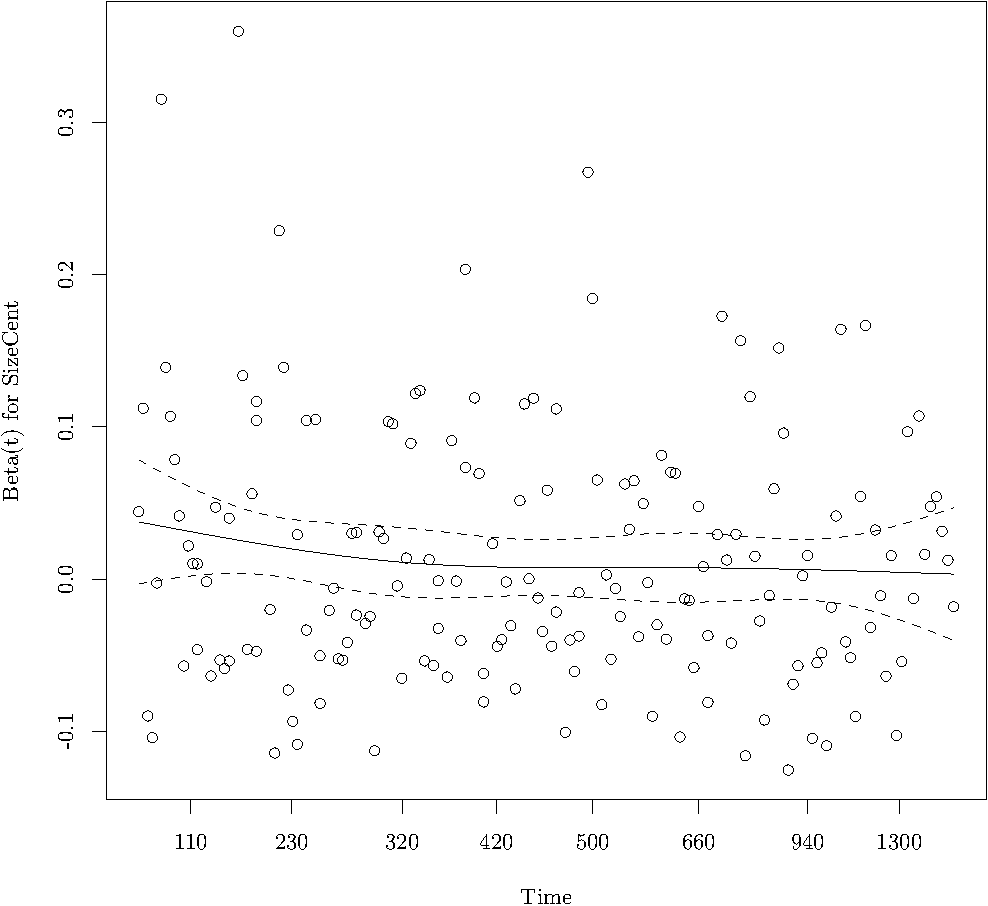
\includegraphics[width=\maxwidth]{figure/05-eda-ph-check-reduced-1} 

}




{\centering 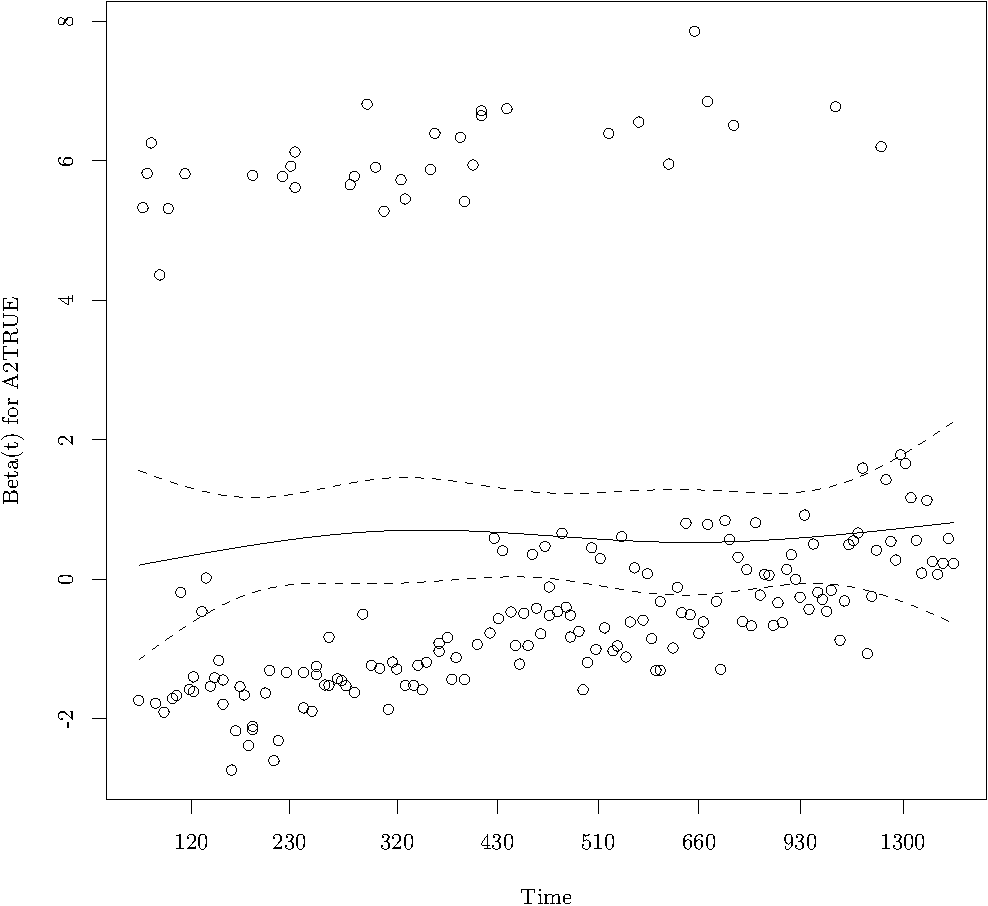
\includegraphics[width=\maxwidth]{figure/05-eda-ph-check-reduced-2} 

}




{\centering 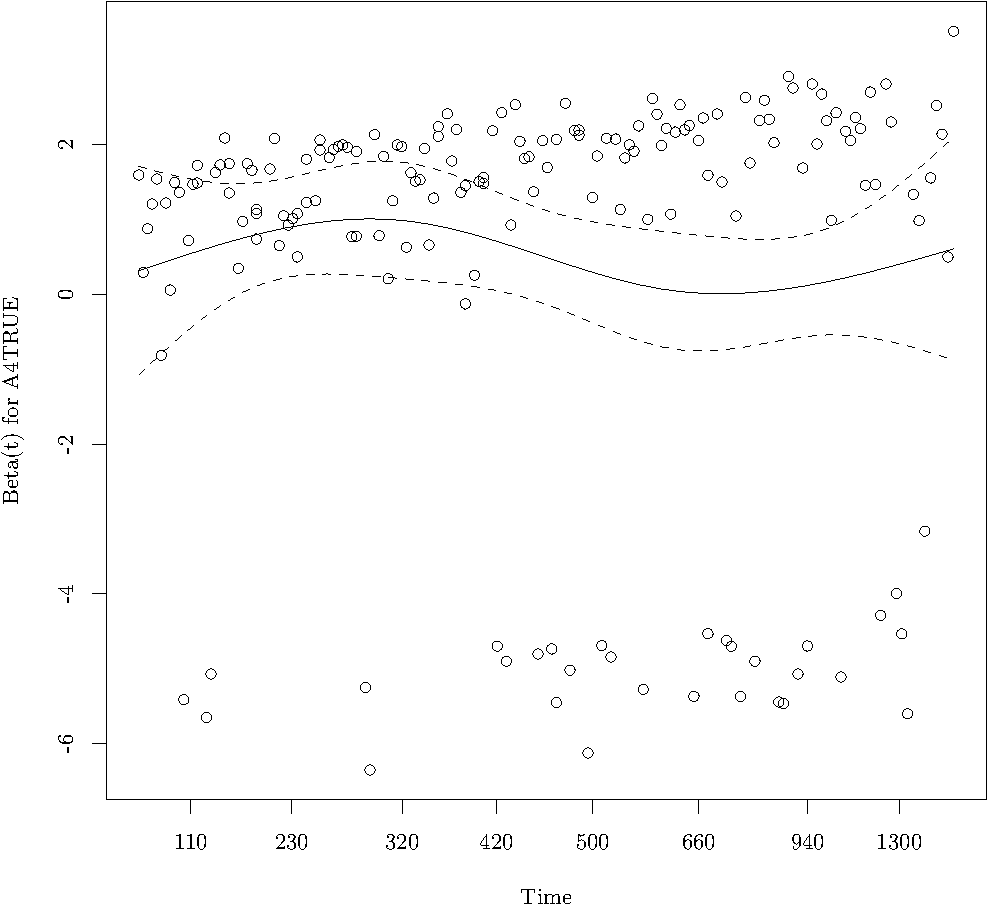
\includegraphics[width=\maxwidth]{figure/05-eda-ph-check-reduced-3} 

}



\end{knitrout}
Interesting effect on A4.  Betas for A4+ drop at high times.  Could this suggest that high A4 is a met proxy, but \emph{not always} -- there are some A4+ pts who don't met, and thus once they've made it to 800 days or so (by which point the mets should have killed them), they're proven to have a met-free high-A4 phenotype, and consequently have good survival?

Size also has a bit of a non-PH indication, but I'm not particularly fussed as it's graphically not too worrying.

For now maybe just stratify by A4 and be done with it.
\begin{knitrout}
\definecolor{shadecolor}{rgb}{0.969, 0.969, 0.969}\color{fgcolor}\begin{kframe}
\begin{alltt}
\hlstd{fit.cph} \hlkwb{=} \hlkwd{coxph}\hlstd{(}\hlkwd{Surv}\hlstd{(Time, DSD)} \hlopt{~} \hlstd{SizeCent} \hlopt{+} \hlstd{A2} \hlopt{+} \hlkwd{strata}\hlstd{(A4),} \hlkwc{data} \hlstd{= data)}
\hlkwd{cox.zph}\hlstd{(fit.cph)}
\end{alltt}
\begin{verbatim}
##              rho chisq      p
## SizeCent -0.1384 3.607 0.0575
## A2TRUE   -0.0415 0.318 0.5727
## GLOBAL        NA 4.198 0.1226
\end{verbatim}
\begin{alltt}
\hlkwd{plot}\hlstd{(}\hlkwd{cox.zph}\hlstd{(fit.cph))}
\end{alltt}
\end{kframe}

{\centering 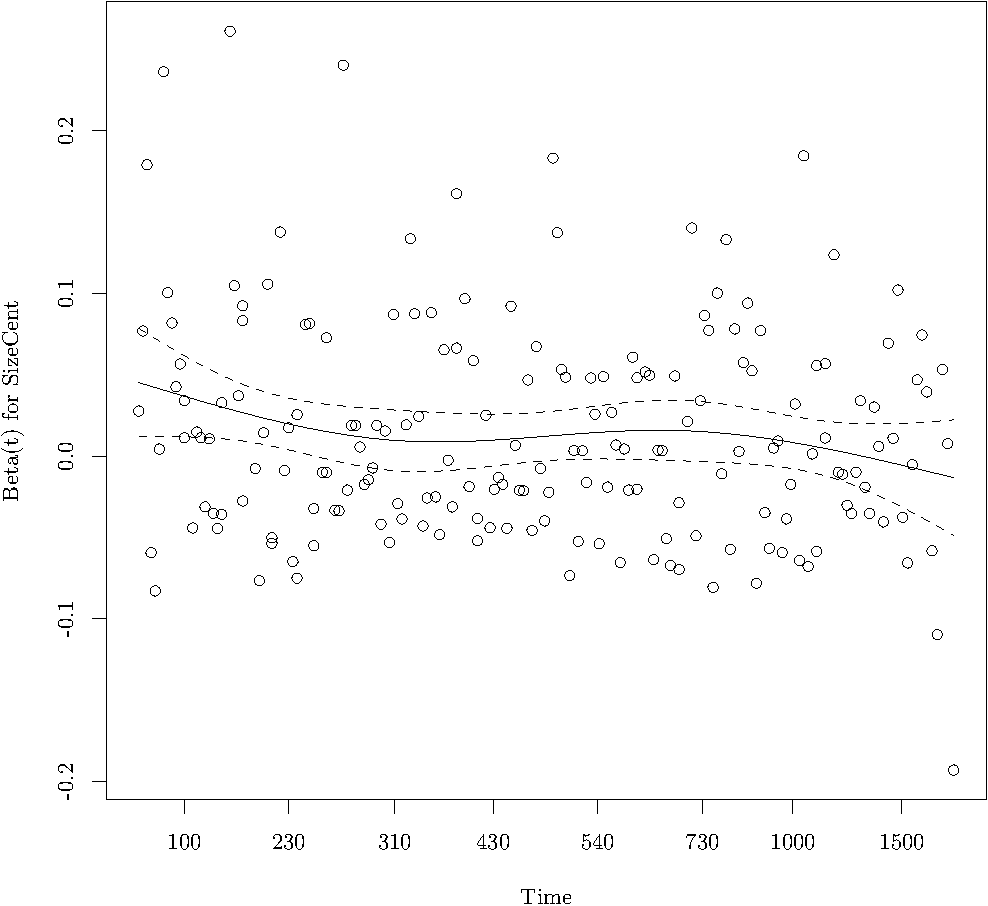
\includegraphics[width=\maxwidth]{figure/05-eda-final-fit-1} 

}




{\centering 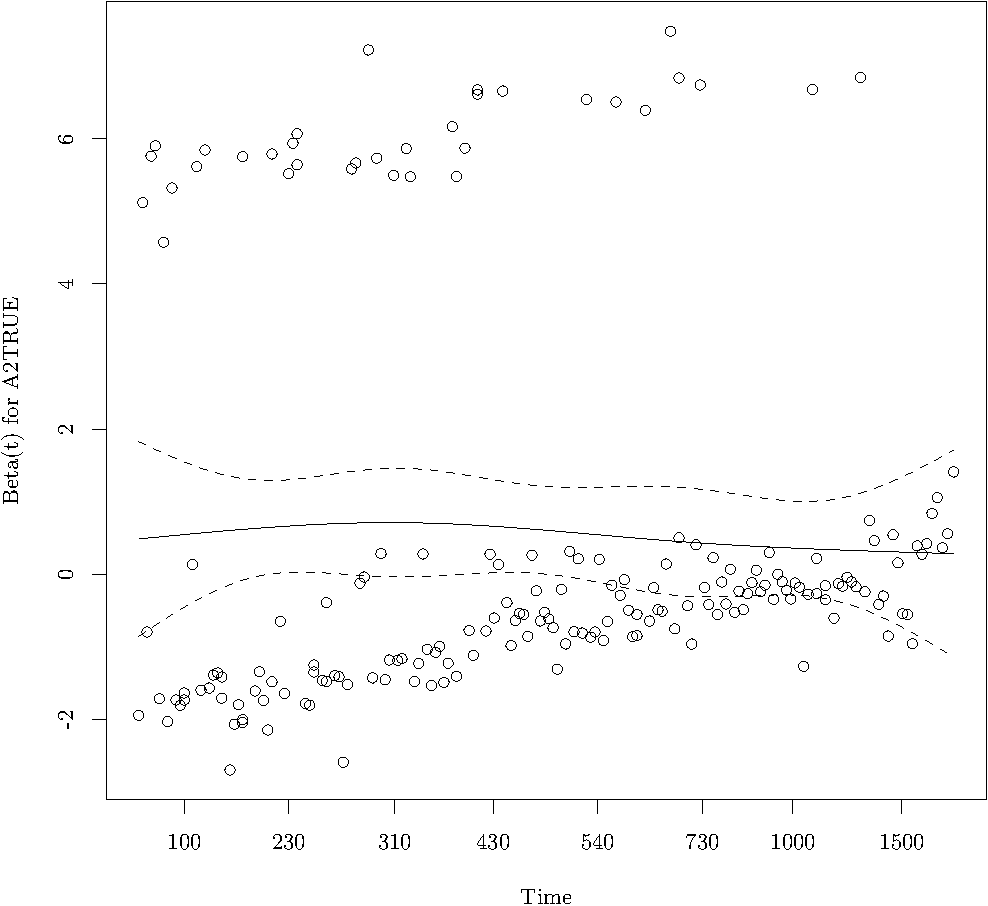
\includegraphics[width=\maxwidth]{figure/05-eda-final-fit-2} 

}



\end{knitrout}


\subsection{Outliers: reduced model}
\begin{knitrout}
\definecolor{shadecolor}{rgb}{0.969, 0.969, 0.969}\color{fgcolor}\begin{kframe}
\begin{alltt}
\hlkwd{scatter.smooth}\hlstd{(}\hlkwd{resid}\hlstd{(fit.cph,} \hlkwc{type} \hlstd{=} \hlstr{"deviance"}\hlstd{), data}\hlopt{$}\hlstd{SizeCent,} \hlkwc{xlab} \hlstd{=} \hlstr{"SizeCent"}\hlstd{,} \hlkwc{main} \hlstd{=} \hlstr{"Deviance vs SizeCent"}\hlstd{,} \hlkwc{ylab} \hlstd{=} \hlstr{"Deviance residuals"}\hlstd{)}
\end{alltt}
\end{kframe}

{\centering 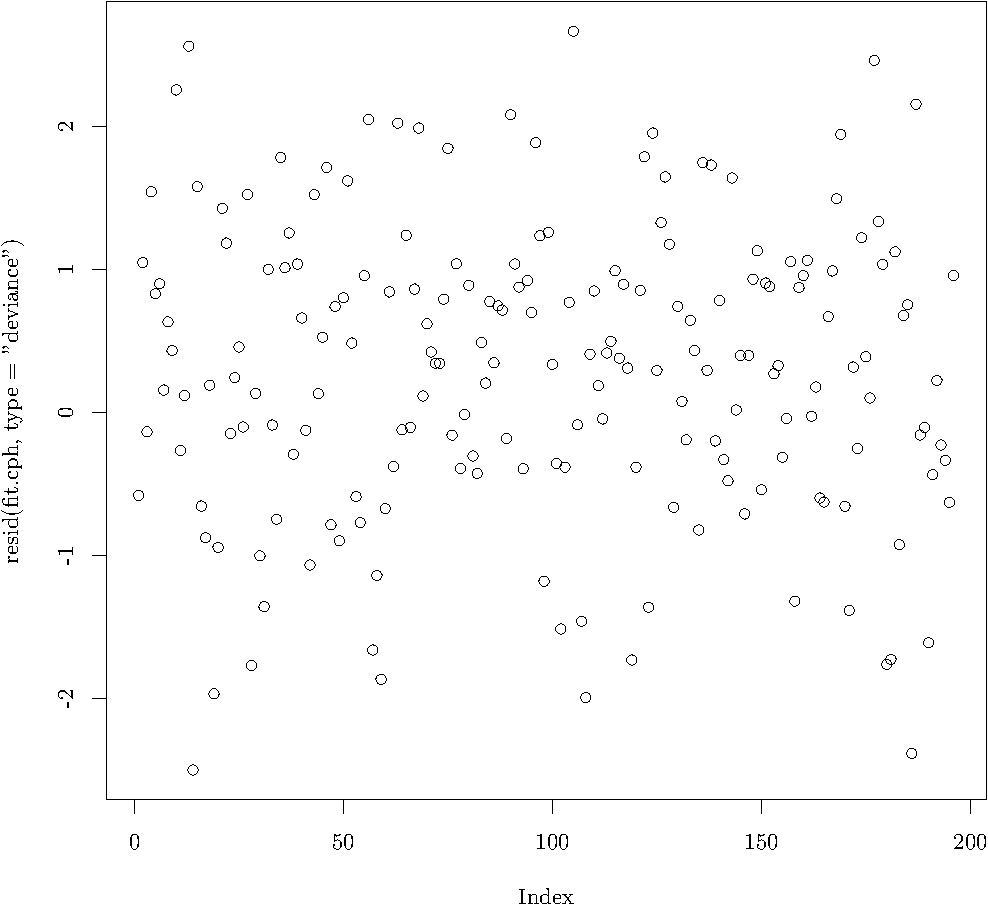
\includegraphics[width=\maxwidth]{figure/05-eda-outliers-reduced-1} 

}


\begin{kframe}\begin{alltt}
\hlkwd{boxplot}\hlstd{(}\hlkwd{resid}\hlstd{(fit.cph,} \hlkwc{type} \hlstd{=} \hlstr{"deviance"}\hlstd{)} \hlopt{~} \hlstd{data}\hlopt{$}\hlstd{A2,} \hlkwc{main} \hlstd{=} \hlstr{"Deviance vs A2"}\hlstd{,} \hlkwc{xlab} \hlstd{=} \hlstr{"A2"}\hlstd{,} \hlkwc{ylab} \hlstd{=} \hlstr{"Deviance residuals"}\hlstd{)}
\end{alltt}
\end{kframe}

{\centering 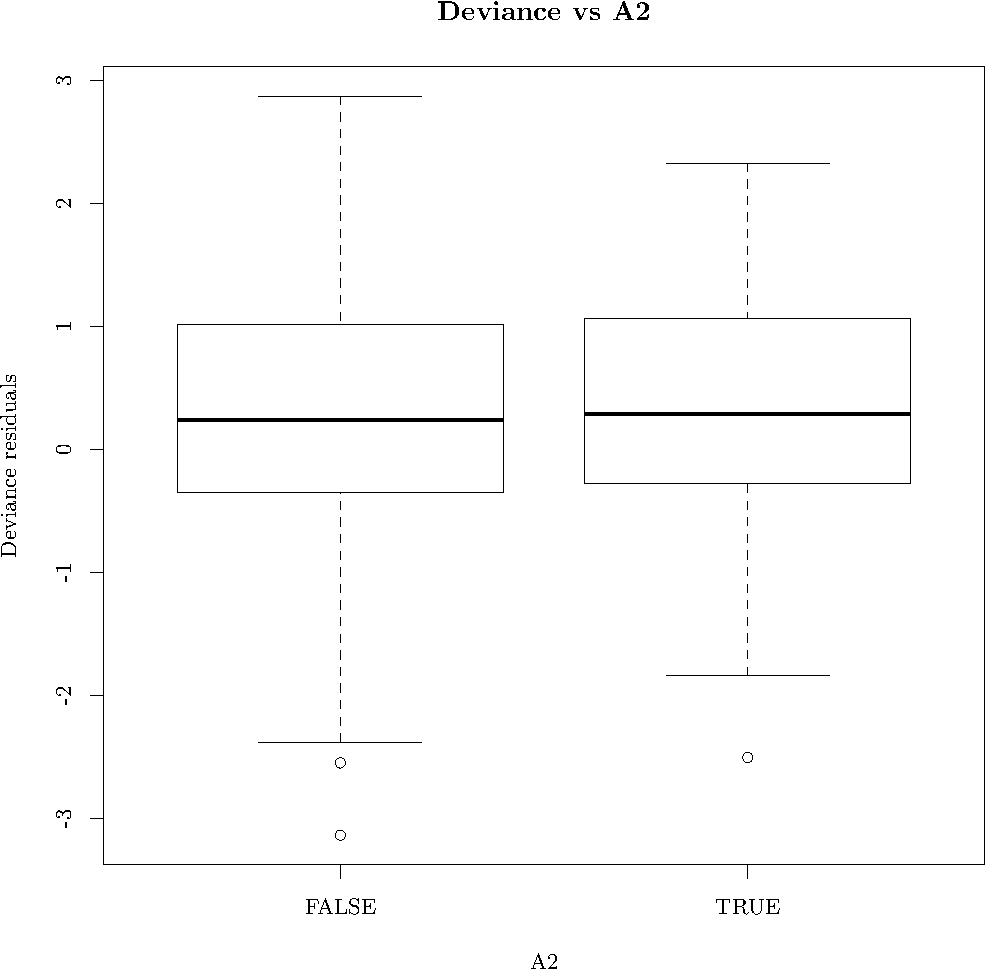
\includegraphics[width=\maxwidth]{figure/05-eda-outliers-reduced-2} 

}


\begin{kframe}\begin{alltt}
\hlkwd{boxplot}\hlstd{(}\hlkwd{resid}\hlstd{(fit.cph,} \hlkwc{type} \hlstd{=} \hlstr{"deviance"}\hlstd{)} \hlopt{~} \hlstd{data}\hlopt{$}\hlstd{A4,} \hlkwc{main} \hlstd{=} \hlstr{"Deviance vs A4"}\hlstd{,} \hlkwc{xlab} \hlstd{=} \hlstr{"A4"}\hlstd{,} \hlkwc{ylab} \hlstd{=} \hlstr{"Deviance residuals"}\hlstd{)}
\end{alltt}
\end{kframe}

{\centering 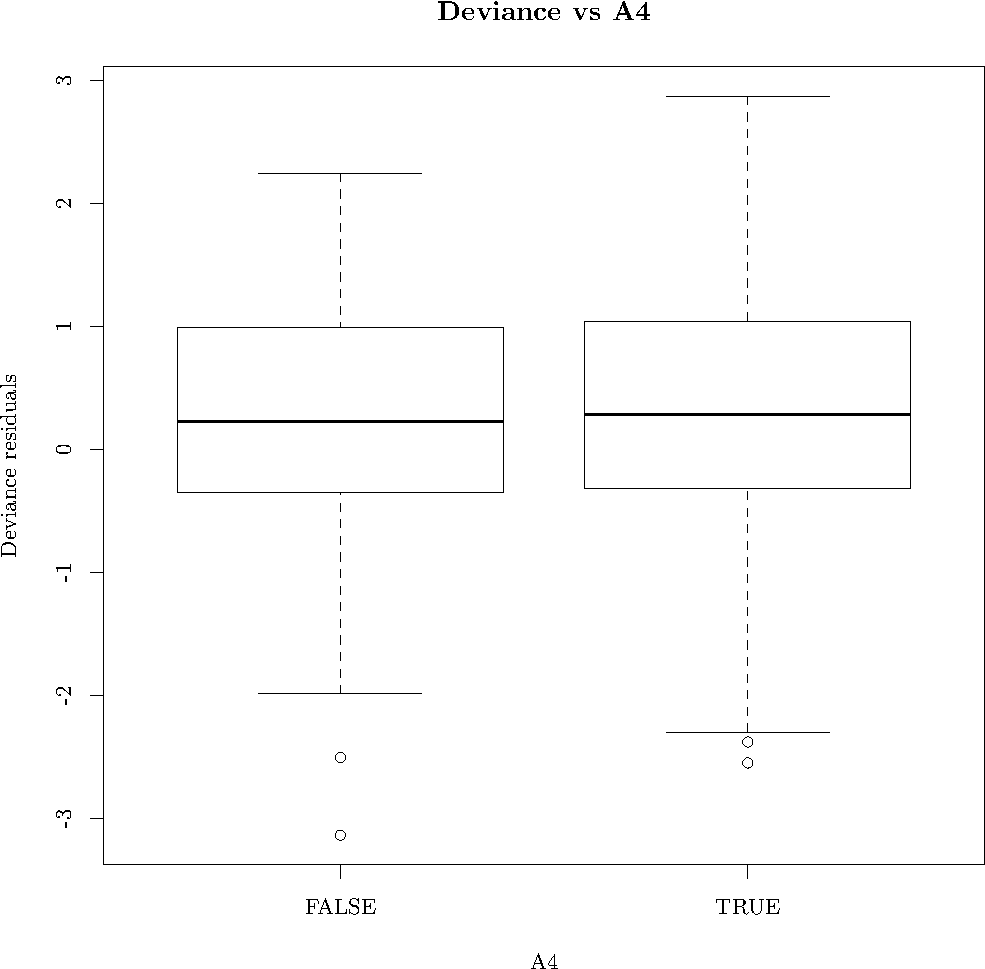
\includegraphics[width=\maxwidth]{figure/05-eda-outliers-reduced-3} 

}


\begin{kframe}\begin{alltt}
\hlkwd{plot}\hlstd{(}\hlkwd{resid}\hlstd{(fit.cph,} \hlkwc{type} \hlstd{=} \hlstr{"deviance"}\hlstd{))}
\hlkwd{abline}\hlstd{(}\hlkwc{h} \hlstd{=} \hlkwd{c}\hlstd{(}\hlopt{-}\hlnum{2.5}\hlstd{,} \hlnum{2.5}\hlstd{))}
\end{alltt}
\end{kframe}

{\centering 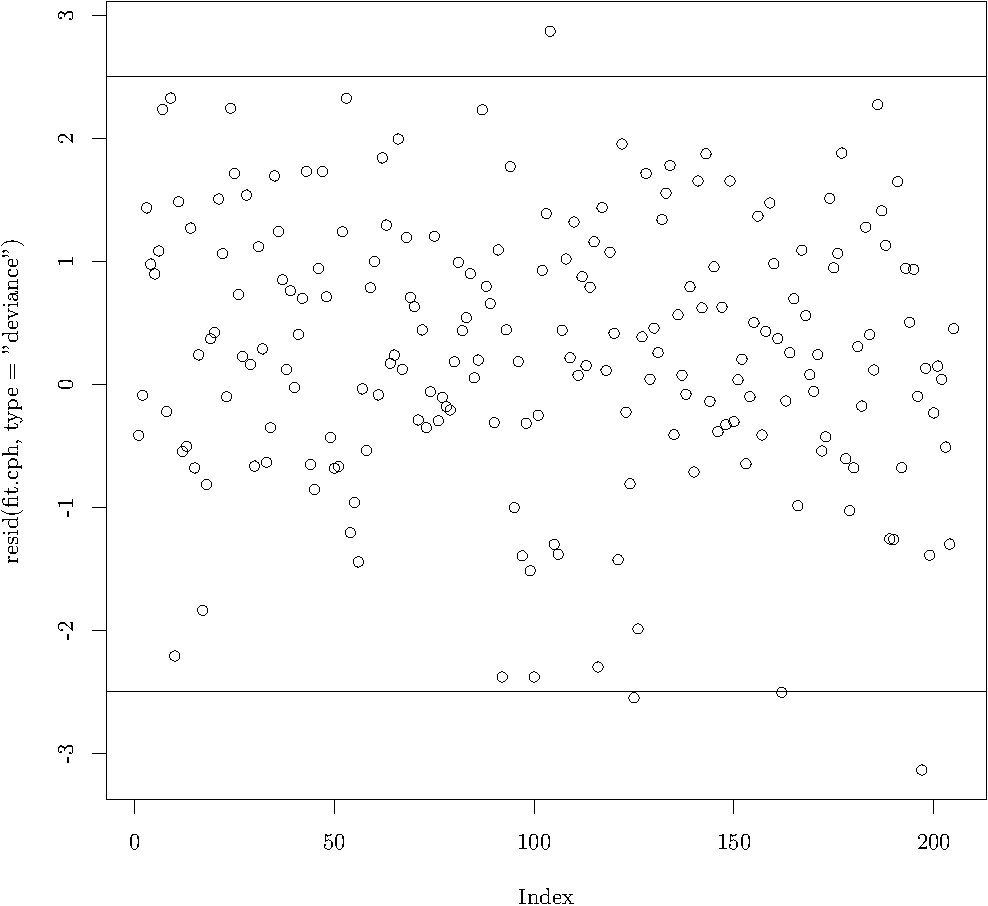
\includegraphics[width=\maxwidth]{figure/05-eda-outliers-reduced-4} 

}


\begin{kframe}\begin{alltt}
\hlstd{data}\hlopt{$}\hlstd{devresid} \hlkwb{=} \hlkwd{resid}\hlstd{(fit.cph,} \hlkwc{type} \hlstd{=} \hlstr{"deviance"}\hlstd{)}
\hlstd{temp} \hlkwb{=} \hlstd{data[}\hlkwd{abs}\hlstd{(data}\hlopt{$}\hlstd{devresid)} \hlopt{>=} \hlnum{2.5}\hlstd{,]}
\hlstd{temp[}\hlkwd{order}\hlstd{(temp}\hlopt{$}\hlstd{Time),]}
\end{alltt}
\begin{verbatim}
##             Time   DSD  SexM AgeCent LocBody SizeCent    A2    A4 AgePlus
## NSWPCN_651    20  TRUE  TRUE       8    TRUE       10 FALSE  TRUE       8
## NSWPCN_1095 1836 FALSE  TRUE      -8   FALSE        0  TRUE FALSE       0
## NSWPCN_787  3287 FALSE FALSE       3   FALSE        0 FALSE  TRUE       3
## NSWPCN_1203 5063 FALSE FALSE       5    TRUE       45 FALSE FALSE       5
##             SizePlus devresid
## NSWPCN_651        10    2.871
## NSWPCN_1095        0   -2.504
## NSWPCN_787         0   -2.548
## NSWPCN_1203       45   -3.135
\end{verbatim}
\end{kframe}
\end{knitrout}
Few enough that I'm not particularly concerned.  The DFBETAS will be more telling.

\begin{knitrout}
\definecolor{shadecolor}{rgb}{0.969, 0.969, 0.969}\color{fgcolor}\begin{kframe}
\begin{alltt}
\hlstd{temp} \hlkwb{=} \hlkwd{resid}\hlstd{(fit.cph,} \hlkwc{type} \hlstd{=} \hlstr{"dfbetas"}\hlstd{)}
\hlkwd{colnames}\hlstd{(temp)} \hlkwb{=} \hlkwd{names}\hlstd{(fit.cph}\hlopt{$}\hlstd{coefficients)}
\hlstd{temp} \hlkwb{=} \hlkwd{melt}\hlstd{(temp)}
\hlkwd{colnames}\hlstd{(temp)} \hlkwb{=} \hlkwd{c}\hlstd{(}\hlstr{"Patient"}\hlstd{,} \hlstr{"Coefficient"}\hlstd{,} \hlstr{"dfbetas"}\hlstd{)}
\hlstd{temp}\hlopt{$}\hlstd{Patient} \hlkwb{=} \hlkwd{gsub}\hlstd{(}\hlstr{"NSWPCN_"}\hlstd{,} \hlstr{""}\hlstd{, temp}\hlopt{$}\hlstd{Patient)}
\hlnum{2}\hlopt{/}\hlkwd{sqrt}\hlstd{(}\hlkwd{nrow}\hlstd{(data))}              \hlcom{# The classic threshold for concern is 2/sqrt(n).}
\end{alltt}
\begin{verbatim}
## [1] 0.1397
\end{verbatim}
\begin{alltt}
\hlkwd{ggplot}\hlstd{(temp,} \hlkwd{aes}\hlstd{(}\hlkwc{y} \hlstd{=} \hlkwd{abs}\hlstd{(dfbetas),} \hlkwc{x} \hlstd{= Patient,} \hlkwc{col} \hlstd{= Coefficient))} \hlopt{+} \hlkwd{geom_point}\hlstd{()} \hlopt{+} \hlkwd{geom_hline}\hlstd{(}\hlkwc{yintercept} \hlstd{=} \hlnum{2}\hlopt{/}\hlkwd{sqrt}\hlstd{(}\hlkwd{nrow}\hlstd{(data)))}
\end{alltt}
\end{kframe}

{\centering 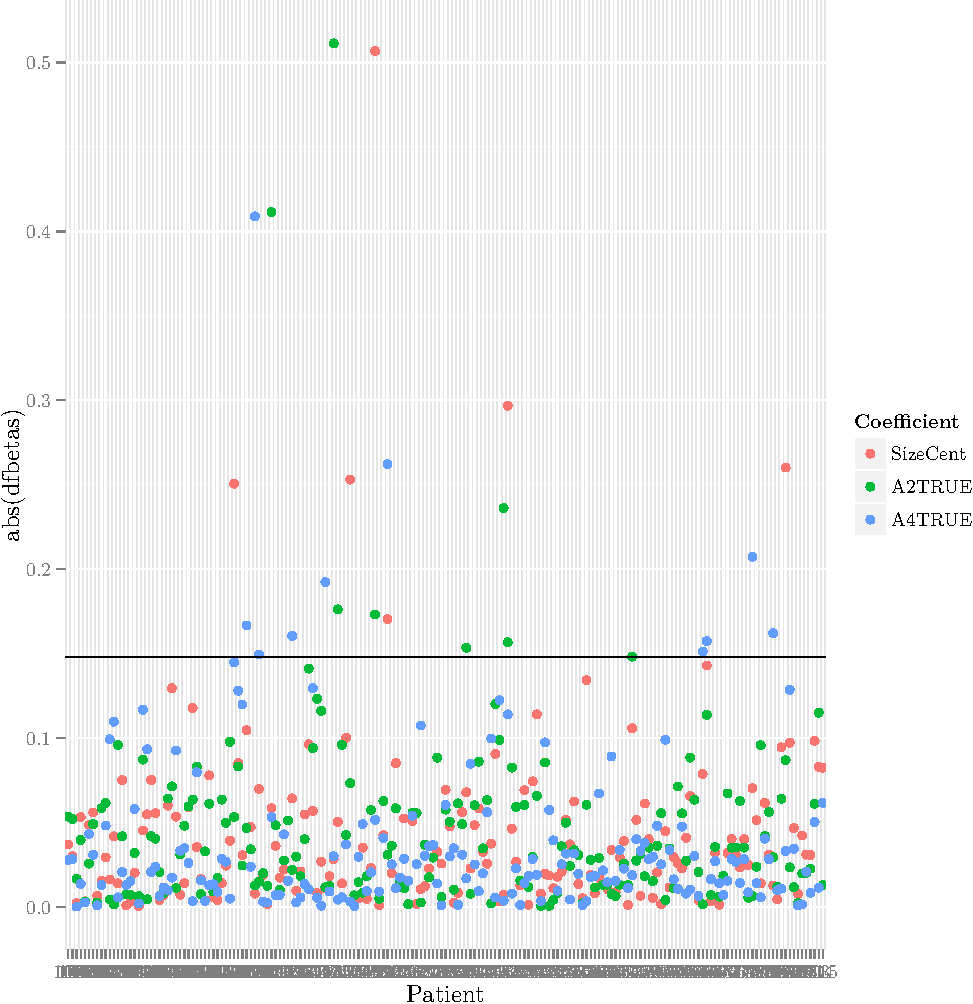
\includegraphics[width=\maxwidth]{figure/05-eda-dfbetas-reduced-1} 

}


\begin{kframe}\begin{alltt}
\hlkwd{sort}\hlstd{(}\hlkwd{apply}\hlstd{(}\hlkwd{abs}\hlstd{(}\hlkwd{resid}\hlstd{(fit.cph,} \hlkwc{type} \hlstd{=} \hlstr{"dfbetas"}\hlstd{)),} \hlnum{1}\hlstd{, max),} \hlkwc{decreasing} \hlstd{=} \hlnum{TRUE}\hlstd{)}
\end{alltt}
\begin{verbatim}
## NSWPCN_1203 NSWPCN_1095  NSWPCN_144 NSWPCN_1253 NSWPCN_1212  NSWPCN_799 
##    0.921541    0.550030    0.481484    0.348056    0.332404    0.208381 
##  NSWPCN_667  NSWPCN_154  NSWPCN_318  NSWPCN_317  NSWPCN_159  NSWPCN_145 
##    0.195400    0.192054    0.186294    0.179351    0.171611    0.141562 
##  NSWPCN_382  NSWPCN_645  NSWPCN_374  NSWPCN_335  NSWPCN_131 NSWPCN_1182 
##    0.140095    0.140095    0.138688    0.137739    0.135884    0.133541 
##  NSWPCN_788  NSWPCN_801 NSWPCN_1083  NSWPCN_315  NSWPCN_135  NSWPCN_814 
##    0.129445    0.121890    0.121601    0.119204    0.116602    0.114628 
##  NSWPCN_296 NSWPCN_1179  NSWPCN_647  NSWPCN_322  NSWPCN_305  NSWPCN_815 
##    0.113348    0.104178    0.099055    0.097116    0.096968    0.089928 
## NSWPCN_1167  NSWPCN_150  NSWPCN_333  NSWPCN_655  NSWPCN_152  NSWPCN_133 
##    0.089197    0.088666    0.088096    0.088029    0.083049    0.081992 
##  NSWPCN_798  NSWPCN_321  NSWPCN_138 NSWPCN_1168  NSWPCN_316  NSWPCN_284 
##    0.080762    0.078351    0.077949    0.077781    0.076806    0.075677 
##  NSWPCN_200  NSWPCN_787  NSWPCN_639  NSWPCN_654 NSWPCN_1143 NSWPCN_1172 
##    0.074404    0.070918    0.070594    0.070312    0.068829    0.068446 
## NSWPCN_1145 NSWPCN_1155 NSWPCN_1186  NSWPCN_651  NSWPCN_326  NSWPCN_813 
##    0.067024    0.066960    0.066370    0.065614    0.060973    0.060895 
##  NSWPCN_125  NSWPCN_304  NSWPCN_648 NSWPCN_1188  NSWPCN_777 NSWPCN_1177 
##    0.060016    0.059777    0.059521    0.059040    0.058506    0.058145 
## NSWPCN_1165  NSWPCN_307  NSWPCN_351  NSWPCN_779  NSWPCN_790  NSWPCN_324 
##    0.057925    0.057738    0.056900    0.056653    0.056494    0.055825 
##  NSWPCN_257 NSWPCN_1017   NSWPCN_10 NSWPCN_1153  NSWPCN_164  NSWPCN_182 
##    0.054462    0.053716    0.052730    0.052435    0.052408    0.051863 
##  NSWPCN_643  NSWPCN_445 NSWPCN_1453 NSWPCN_1082 NSWPCN_1156  NSWPCN_674 
##    0.051850    0.051820    0.051576    0.051541    0.051495    0.051475 
## NSWPCN_1072  NSWPCN_312  NSWPCN_268   NSWPCN_13 NSWPCN_1019  NSWPCN_661 
##    0.051453    0.050800    0.050290    0.049725    0.049718    0.049690 
##  NSWPCN_789  NSWPCN_377 NSWPCN_1089 NSWPCN_1178  NSWPCN_364 NSWPCN_1189 
##    0.048796    0.048647    0.048333    0.048059    0.047965    0.047930 
##  NSWPCN_294 NSWPCN_1023  NSWPCN_802  NSWPCN_256  NSWPCN_320  NSWPCN_141 
##    0.047479    0.047408    0.047161    0.046965    0.046752    0.046576 
## NSWPCN_1075 NSWPCN_1169  NSWPCN_640  NSWPCN_665 NSWPCN_1227  NSWPCN_195 
##    0.044921    0.044725    0.043095    0.040923    0.040635    0.040415 
##  NSWPCN_310 NSWPCN_1029 NSWPCN_1146  NSWPCN_657   NSWPCN_20 NSWPCN_1160 
##    0.039997    0.039927    0.039825    0.038729    0.038275    0.038272 
##  NSWPCN_636 NSWPCN_1140 NSWPCN_1157 NSWPCN_1070  NSWPCN_381  NSWPCN_770 
##    0.038048    0.037796    0.037595    0.037518    0.037410    0.037408 
##  NSWPCN_666  NSWPCN_341  NSWPCN_375  NSWPCN_664  NSWPCN_370  NSWPCN_784 
##    0.037358    0.037181    0.037109    0.036014    0.035322    0.034775 
##  NSWPCN_311 NSWPCN_1193 NSWPCN_1028 NSWPCN_1026  NSWPCN_270  NSWPCN_769 
##    0.034609    0.033846    0.033099    0.032313    0.031357    0.030468 
##  NSWPCN_781  NSWPCN_267 NSWPCN_1187    NSWPCN_4 NSWPCN_1022  NSWPCN_663 
##    0.030153    0.029742    0.029581    0.029355    0.029211    0.029183 
##   NSWPCN_17  NSWPCN_646  NSWPCN_352 NSWPCN_1190  NSWPCN_309  NSWPCN_358 
##    0.028452    0.028383    0.028084    0.027072    0.026056    0.026010 
##  NSWPCN_345 NSWPCN_1171  NSWPCN_348  NSWPCN_775  NSWPCN_804  NSWPCN_126 
##    0.025681    0.025584    0.025263    0.025210    0.024334    0.023897 
## NSWPCN_1018  NSWPCN_807  NSWPCN_269  NSWPCN_810 NSWPCN_1213  NSWPCN_273 
##    0.023702    0.023320    0.023198    0.022445    0.021797    0.021516 
##  NSWPCN_376  NSWPCN_638 NSWPCN_1141  NSWPCN_283  NSWPCN_350 NSWPCN_1207 
##    0.021456    0.020915    0.020888    0.020617    0.020112    0.020022 
##  NSWPCN_353  NSWPCN_662  NSWPCN_157 NSWPCN_1170  NSWPCN_366 NSWPCN_1150 
##    0.019990    0.019073    0.018812    0.018100    0.016987    0.016706 
##  NSWPCN_319    NSWPCN_9  NSWPCN_163  NSWPCN_143  NSWPCN_280 NSWPCN_1215 
##    0.016695    0.016484    0.015964    0.013543    0.013043    0.012612 
##  NSWPCN_360  NSWPCN_332  NSWPCN_373 NSWPCN_1148 NSWPCN_1021  NSWPCN_369 
##    0.012236    0.012209    0.011551    0.011065    0.011027    0.010952 
##  NSWPCN_384  NSWPCN_323  NSWPCN_272  NSWPCN_336  NSWPCN_166 NSWPCN_1027 
##    0.010829    0.010679    0.010525    0.010510    0.010080    0.009928 
##  NSWPCN_806  NSWPCN_363 NSWPCN_1031  NSWPCN_308  NSWPCN_796  NSWPCN_656 
##    0.009815    0.009718    0.009619    0.009611    0.009246    0.009241 
##  NSWPCN_793  NSWPCN_334 NSWPCN_1091 NSWPCN_1139  NSWPCN_136  NSWPCN_190 
##    0.008516    0.008465    0.008244    0.007993    0.007982    0.007815 
## NSWPCN_1176  NSWPCN_372  NSWPCN_330  NSWPCN_344 NSWPCN_1152  NSWPCN_797 
##    0.007445    0.006494    0.004533    0.004262    0.004257    0.004255 
## NSWPCN_1020 NSWPCN_1175 NSWPCN_1222  NSWPCN_142  NSWPCN_658 NSWPCN_1198 
##    0.004037    0.003070    0.002912    0.002600    0.002326    0.002229 
##  NSWPCN_149 
##    0.002201
\end{verbatim}
\begin{alltt}
\hlkwd{sum}\hlstd{(}\hlkwd{apply}\hlstd{(}\hlkwd{abs}\hlstd{(}\hlkwd{resid}\hlstd{(fit.cph,} \hlkwc{type} \hlstd{=} \hlstr{"dfbetas"}\hlstd{)),} \hlnum{1}\hlstd{, max)} \hlopt{>} \hlnum{2}\hlopt{/}\hlkwd{sqrt}\hlstd{(}\hlkwd{nrow}\hlstd{(data)))}
\end{alltt}
\begin{verbatim}
## [1] 14
\end{verbatim}
\begin{alltt}
\hlstd{data}\hlopt{$}\hlstd{DFBETAS_max} \hlkwb{=} \hlkwd{apply}\hlstd{(}\hlkwd{abs}\hlstd{(}\hlkwd{resid}\hlstd{(fit.cph,} \hlkwc{type} \hlstd{=} \hlstr{"dfbetas"}\hlstd{)),} \hlnum{1}\hlstd{, max)}
\hlstd{temp} \hlkwb{=} \hlstd{data[data}\hlopt{$}\hlstd{DFBETAS_max} \hlopt{>=} \hlnum{2}\hlopt{/}\hlkwd{sqrt}\hlstd{(}\hlkwd{nrow}\hlstd{(data))} \hlopt{|} \hlkwd{abs}\hlstd{(data}\hlopt{$}\hlstd{devresid)} \hlopt{>=} \hlnum{2.5}\hlstd{,]}
\hlstd{temp[}\hlkwd{order}\hlstd{(temp}\hlopt{$}\hlstd{DFBETAS_max),]}
\end{alltt}
\begin{verbatim}
##             Time   DSD  SexM AgeCent LocBody SizeCent    A2    A4 AgePlus
## NSWPCN_651    20  TRUE  TRUE       8    TRUE       10 FALSE  TRUE       8
## NSWPCN_787  3287 FALSE FALSE       3   FALSE        0 FALSE  TRUE       3
## NSWPCN_382  4915 FALSE  TRUE     -15   FALSE      -10 FALSE  TRUE       0
## NSWPCN_645  3279 FALSE  TRUE      -6   FALSE      -10 FALSE  TRUE       0
## NSWPCN_145   599  TRUE  TRUE      -6    TRUE       15  TRUE  TRUE       0
## NSWPCN_159    30  TRUE  TRUE      11    TRUE       40 FALSE FALSE      11
## NSWPCN_317   729  TRUE FALSE      11   FALSE       10  TRUE  TRUE      11
## NSWPCN_318  1464  TRUE FALSE       2   FALSE       20 FALSE  TRUE       2
## NSWPCN_154   163  TRUE  TRUE      -2    TRUE       60 FALSE  TRUE       0
## NSWPCN_667  2415 FALSE FALSE     -14   FALSE      -15 FALSE  TRUE       0
## NSWPCN_799    70  TRUE FALSE       4    TRUE       60  TRUE  TRUE       4
## NSWPCN_1212 1053  TRUE  TRUE      12   FALSE        2  TRUE  TRUE      12
## NSWPCN_1253 1044  TRUE  TRUE      -2   FALSE       40 FALSE  TRUE       0
## NSWPCN_144  1206  TRUE FALSE       0   FALSE       10  TRUE  TRUE       0
## NSWPCN_1095 1836 FALSE  TRUE      -8   FALSE        0  TRUE FALSE       0
## NSWPCN_1203 5063 FALSE FALSE       5    TRUE       45 FALSE FALSE       5
##             SizePlus devresid DFBETAS_max
## NSWPCN_651        10   2.8710     0.06561
## NSWPCN_787         0  -2.5481     0.07092
## NSWPCN_382         0  -2.3788     0.14010
## NSWPCN_645         0  -2.3788     0.14010
## NSWPCN_145        15  -0.8134     0.14156
## NSWPCN_159        40   2.2447     0.17161
## NSWPCN_317        10  -0.9593     0.17935
## NSWPCN_318        20  -1.4433     0.18629
## NSWPCN_154        60   1.0620     0.19205
## NSWPCN_667         0  -2.2984     0.19540
## NSWPCN_799        60   1.5536     0.20838
## NSWPCN_1212        2  -1.3883     0.33240
## NSWPCN_1253       40  -1.2988     0.34806
## NSWPCN_144        10  -1.8368     0.48148
## NSWPCN_1095        0  -2.5042     0.55003
## NSWPCN_1203       45  -3.1354     0.92154
\end{verbatim}
\end{kframe}
\end{knitrout}
Some long survivors are causing problems.  Given the data issues, it'd be prudent to remove them -- it's not
practical to go back to the source data and find out if they're legit or not.  These guys are alive at >10 years,
according to the data, which is near unheard-of in PDAC.  I propose to remove all pts alive for 3000 days or longer, and
anything with DFBETAS >= 0.2.

\begin{knitrout}
\definecolor{shadecolor}{rgb}{0.969, 0.969, 0.969}\color{fgcolor}\begin{kframe}
\begin{alltt}
\hlstd{data} \hlkwb{=} \hlstd{data[data}\hlopt{$}\hlstd{Time} \hlopt{<} \hlnum{3000} \hlopt{&} \hlstd{data}\hlopt{$}\hlstd{DFBETAS_max} \hlopt{<} \hlnum{0.2}\hlstd{,]}
\hlstd{data.val} \hlkwb{=} \hlstd{data.val[data.val}\hlopt{$}\hlstd{Time} \hlopt{<} \hlnum{3000}\hlstd{,]}
\end{alltt}
\end{kframe}
\end{knitrout}

Now repeat everything...
\subsection{Functional form}
\begin{knitrout}
\definecolor{shadecolor}{rgb}{0.969, 0.969, 0.969}\color{fgcolor}\begin{kframe}
\begin{alltt}
\hlstd{fit.cph.NoAge} \hlkwb{=} \hlkwd{coxph}\hlstd{(}\hlkwd{Surv}\hlstd{(Time, DSD)} \hlopt{~} \hlstd{SexM} \hlopt{+} \hlstd{LocBody} \hlopt{+} \hlstd{SizeCent} \hlopt{+} \hlstd{A2} \hlopt{+} \hlstd{A4,} \hlkwc{data} \hlstd{= data)}
\hlkwd{scatter.smooth}\hlstd{(data}\hlopt{$}\hlstd{AgeCent,} \hlkwd{resid}\hlstd{(fit.cph.NoAge,} \hlkwc{type} \hlstd{=} \hlstr{"martingale"}\hlstd{),} \hlkwc{xlab} \hlstd{=} \hlstr{""}\hlstd{,} \hlkwc{ylab} \hlstd{=} \hlstr{"Martingale residual"}\hlstd{)}
\end{alltt}
\end{kframe}

{\centering 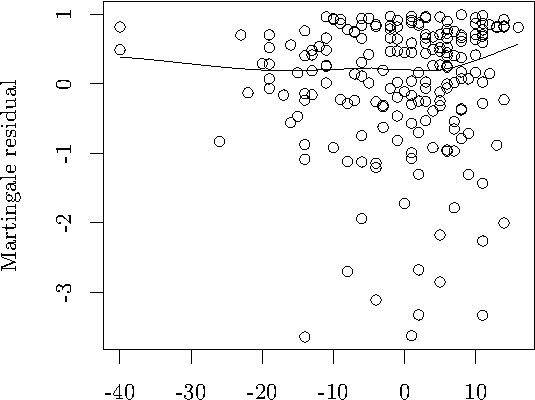
\includegraphics[width=\maxwidth]{figure/05-eda-func-form-age-2-1} 

}


\begin{kframe}\begin{alltt}
\hlkwd{scatter.smooth}\hlstd{(data}\hlopt{$}\hlstd{AgeCent,} \hlkwd{resid}\hlstd{(fit.cph.NoAge,} \hlkwc{type} \hlstd{=} \hlstr{"martingale"}\hlstd{),} \hlkwc{xlab} \hlstd{=} \hlstr{""}\hlstd{,} \hlkwc{ylab} \hlstd{=} \hlstr{"Martingale residual"}\hlstd{,} \hlkwc{ylim} \hlstd{=} \hlkwd{c}\hlstd{(}\hlopt{-}\hlnum{1}\hlstd{,} \hlnum{1}\hlstd{))}
\end{alltt}
\end{kframe}

{\centering 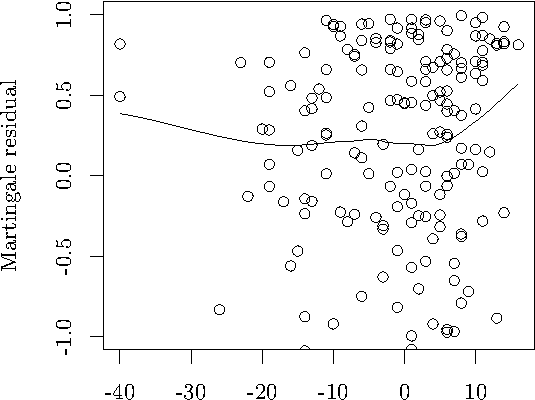
\includegraphics[width=\maxwidth]{figure/05-eda-func-form-age-2-2} 

}



\end{knitrout}

\begin{knitrout}
\definecolor{shadecolor}{rgb}{0.969, 0.969, 0.969}\color{fgcolor}\begin{kframe}
\begin{alltt}
\hlstd{fit.cph.NoSize} \hlkwb{=} \hlkwd{coxph}\hlstd{(}\hlkwd{Surv}\hlstd{(Time, DSD)} \hlopt{~} \hlstd{SexM} \hlopt{+} \hlstd{AgeCent} \hlopt{+} \hlstd{LocBody} \hlopt{+} \hlstd{A2} \hlopt{+} \hlstd{A4,} \hlkwc{data} \hlstd{= data)}
\hlkwd{scatter.smooth}\hlstd{(data}\hlopt{$}\hlstd{SizeCent,} \hlkwd{resid}\hlstd{(fit.cph.NoSize,} \hlkwc{type} \hlstd{=} \hlstr{"martingale"}\hlstd{),} \hlkwc{xlab} \hlstd{=} \hlstr{""}\hlstd{,} \hlkwc{ylab} \hlstd{=} \hlstr{"Martingale residual"}\hlstd{)}
\end{alltt}
\end{kframe}

{\centering 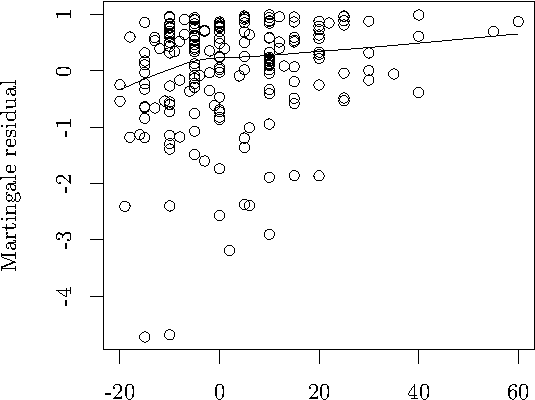
\includegraphics[width=\maxwidth]{figure/05-eda-func-form-size-2-1} 

}


\begin{kframe}\begin{alltt}
\hlkwd{scatter.smooth}\hlstd{(data}\hlopt{$}\hlstd{SizeCent,} \hlkwd{resid}\hlstd{(fit.cph.NoSize,} \hlkwc{type} \hlstd{=} \hlstr{"martingale"}\hlstd{),} \hlkwc{xlab} \hlstd{=} \hlstr{""}\hlstd{,} \hlkwc{ylab} \hlstd{=} \hlstr{"Martingale residual"}\hlstd{,} \hlkwc{ylim} \hlstd{=} \hlkwd{c}\hlstd{(}\hlopt{-}\hlnum{1}\hlstd{,} \hlnum{1}\hlstd{))}
\end{alltt}
\end{kframe}

{\centering 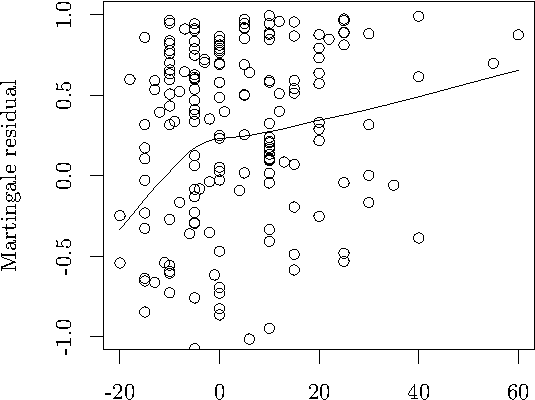
\includegraphics[width=\maxwidth]{figure/05-eda-func-form-size-2-2} 

}



\end{knitrout}
It looks like age has a minor nonlinear component, with a small uptick at advanced age.  Very minor though.  The size relationship appears to have a knee, close to size == 0, around which the relationship is approximately linear.

Model age as:  $AgeCent + AgeCent I(AgeCent > 0) \equiv AgeCent+ AgeCent_+$
Model size as: $SizeCent + SizeCent I(SizeCent > 0) \equiv SizeCent + SizeCent_+$

\begin{knitrout}
\definecolor{shadecolor}{rgb}{0.969, 0.969, 0.969}\color{fgcolor}\begin{kframe}
\begin{alltt}
\hlstd{data}\hlopt{$}\hlstd{AgePlus} \hlkwb{=} \hlkwd{pmax}\hlstd{(data}\hlopt{$}\hlstd{AgeCent,} \hlnum{5}\hlstd{)} \hlopt{-} \hlnum{5}
\hlstd{data}\hlopt{$}\hlstd{SizePlus} \hlkwb{=} \hlkwd{pmax}\hlstd{(data}\hlopt{$}\hlstd{SizeCent,} \hlnum{0}\hlstd{)}
\end{alltt}
\end{kframe}
\end{knitrout}


\subsection{PH assumption: full model}
\begin{knitrout}
\definecolor{shadecolor}{rgb}{0.969, 0.969, 0.969}\color{fgcolor}\begin{kframe}
\begin{alltt}
\hlstd{fit.cph} \hlkwb{=} \hlkwd{coxph}\hlstd{(}\hlkwd{Surv}\hlstd{(Time, DSD)} \hlopt{~} \hlstd{SexM} \hlopt{+} \hlstd{AgeCent} \hlopt{+} \hlstd{AgePlus} \hlopt{+} \hlstd{LocBody} \hlopt{+} \hlstd{SizeCent} \hlopt{+} \hlstd{SizePlus} \hlopt{+} \hlstd{A2} \hlopt{+} \hlstd{A4,} \hlkwc{data} \hlstd{= data)}
\hlkwd{cox.zph}\hlstd{(fit.cph)}
\end{alltt}
\begin{verbatim}
##                 rho   chisq      p
## SexMTRUE     0.1781  6.1794 0.0129
## AgeCent     -0.0276  0.1590 0.6900
## AgePlus     -0.0653  0.9177 0.3381
## LocBodyTRUE -0.1213  2.5855 0.1078
## SizeCent    -0.0205  0.0798 0.7776
## SizePlus     0.0378  0.2999 0.5840
## A2TRUE       0.0973  1.9176 0.1661
## A4TRUE      -0.1033  1.9860 0.1588
## GLOBAL           NA 15.9230 0.0435
\end{verbatim}
\begin{alltt}
\hlkwd{plot}\hlstd{(}\hlkwd{cox.zph}\hlstd{(fit.cph)[}\hlnum{1}\hlstd{])}
\end{alltt}
\end{kframe}

{\centering 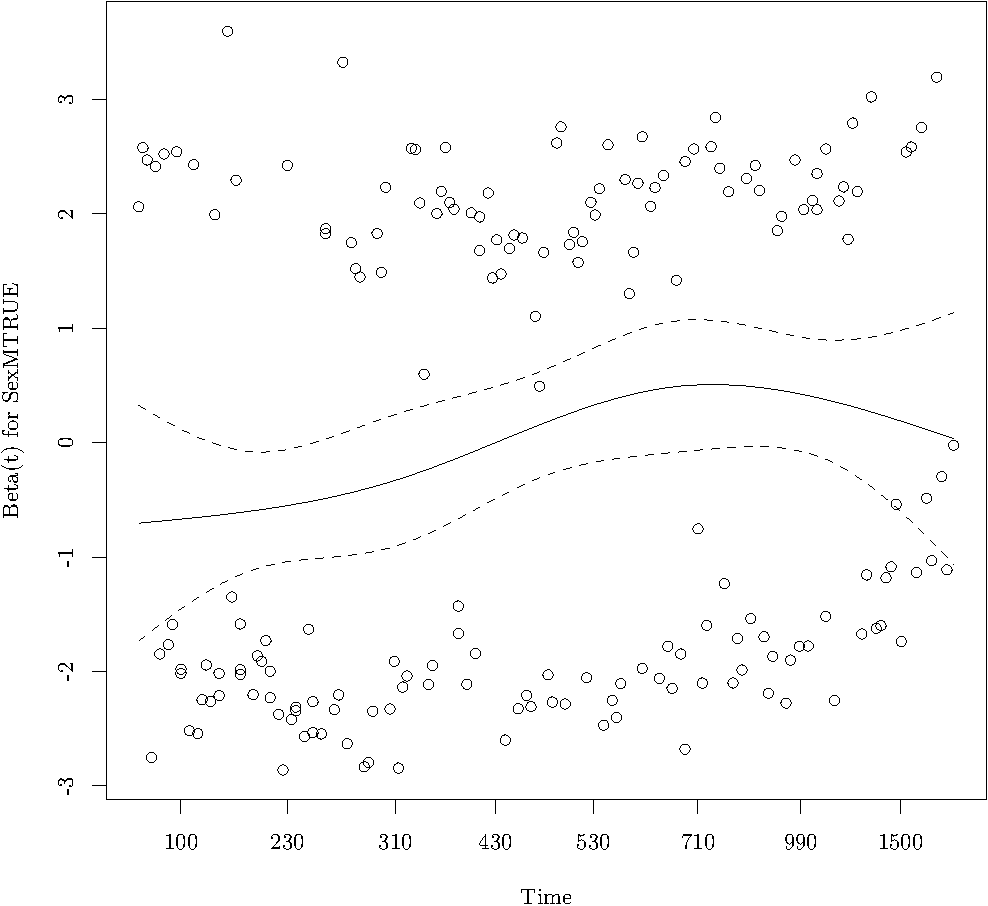
\includegraphics[width=\maxwidth]{figure/05-eda-ph-check-full-2-1} 

}



\end{knitrout}


\subsection{EDA: Variable selection}
\begin{knitrout}
\definecolor{shadecolor}{rgb}{0.969, 0.969, 0.969}\color{fgcolor}\begin{kframe}
\begin{alltt}
\hlstd{nobs.coxph} \hlkwb{<<-} \hlkwa{function}\hlstd{(}\hlkwc{obj}\hlstd{,} \hlkwc{...}\hlstd{)} \hlkwd{sum}\hlstd{(obj}\hlopt{$}\hlstd{y[,}\hlnum{2}\hlstd{])}
\hlkwd{set.seed}\hlstd{(}\hlnum{20150201}\hlstd{)}
\hlstd{fit.cph.as.bic} \hlkwb{=} \hlkwd{glmulti}\hlstd{(}\hlkwd{Surv}\hlstd{(Time, DSD)} \hlopt{~} \hlkwd{strata}\hlstd{(SexM)} \hlopt{+} \hlstd{AgeCent} \hlopt{+} \hlstd{AgePlus} \hlopt{+} \hlstd{LocBody} \hlopt{+} \hlstd{SizeCent} \hlopt{+} \hlstd{SizePlus} \hlopt{+} \hlstd{A2} \hlopt{+} \hlstd{A4,} \hlkwc{data} \hlstd{= data,} \hlkwc{marginality} \hlstd{=} \hlnum{TRUE}\hlstd{,} \hlkwc{method} \hlstd{=} \hlstr{"g"}\hlstd{,} \hlkwc{fitfunction} \hlstd{=} \hlstr{"coxph"}\hlstd{,} \hlkwc{crit} \hlstd{=} \hlstr{"bic"}\hlstd{,} \hlkwc{level} \hlstd{=} \hlnum{2}\hlstd{,} \hlkwc{plotty} \hlstd{=} \hlnum{FALSE}\hlstd{,} \hlkwc{report} \hlstd{=} \hlnum{TRUE}\hlstd{)}
\end{alltt}
\begin{verbatim}
## Initialization...
## TASK: Genetic algorithm in the candidate set.
## Initialization...
## Algorithm started...
## 
## After 10 generations:
## Best model: Surv(Time,DSD)~1+strata(SexM)+AgeCent+AgePlus+LocBody+SizeCent+SizePlus+A2+A4+AgePlus:AgeCent+LocBody:AgeCent+SizeCent:AgePlus+SizePlus:LocBody+A2:SizeCent+A4:AgeCent+strata(SexM):SizeCent
## Crit= 1386.45949115679
## Mean crit= 1417.52264128484
## Change in best IC: -8613.54050884321 / Change in mean IC: -8582.47735871516
## 
## After 20 generations:
## Best model: Surv(Time,DSD)~1+strata(SexM)+AgePlus+LocBody+SizeCent+A2+A4+A2:SizeCent+A4:LocBody+strata(SexM):SizeCent
## Crit= 1361.32514921699
## Mean crit= 1410.127136962
## Change in best IC: -25.1343419398004 / Change in mean IC: -7.39550432283295
\end{verbatim}


{\ttfamily\noindent\color{warningcolor}{\#\# Warning in fitter(X, Y, strats, offset, init, control, weights = weights, : Loglik converged before variable\ \ 11 ; beta may be infinite.}}\begin{verbatim}
## 
## After 30 generations:
## Best model: Surv(Time,DSD)~1+strata(SexM)+LocBody+SizeCent+A2+A4+A4:LocBody+strata(SexM):SizeCent
## Crit= 1353.38950302717
## Mean crit= 1406.8093174039
## Change in best IC: -7.93564618981941 / Change in mean IC: -3.31781955810561
## 
## After 40 generations:
## Best model: Surv(Time,DSD)~1+strata(SexM)+LocBody+SizeCent+A2+A4+A4:LocBody
## Crit= 1352.59611072079
## Mean crit= 1403.67123867365
## Change in best IC: -0.793392306378109 / Change in mean IC: -3.13807873024439
## 
## After 50 generations:
## Best model: Surv(Time,DSD)~1+strata(SexM)+LocBody+SizeCent+A2+A4
## Crit= 1347.65885958051
## Mean crit= 1401.35223231976
## Change in best IC: -4.93725114028302 / Change in mean IC: -2.3190063538982
## 
## After 60 generations:
## Best model: Surv(Time,DSD)~1+strata(SexM)+LocBody+SizeCent+A2+A4
## Crit= 1347.65885958051
## Mean crit= 1400.20683837434
## Change in best IC: 0 / Change in mean IC: -1.1453939454118
## 
## After 70 generations:
## Best model: Surv(Time,DSD)~1+strata(SexM)+SizeCent+A2+A4
## Crit= 1342.43618902348
## Mean crit= 1398.35960553043
## Change in best IC: -5.22267055702287 / Change in mean IC: -1.84723284391066
## 
## After 80 generations:
## Best model: Surv(Time,DSD)~1+strata(SexM)+SizeCent+A2+A4
## Crit= 1342.43618902348
## Mean crit= 1396.84197554499
## Change in best IC: 0 / Change in mean IC: -1.51762998543973
## 
## After 90 generations:
## Best model: Surv(Time,DSD)~1+strata(SexM)+SizeCent+A2+A4
## Crit= 1342.43618902348
## Mean crit= 1395.23823697744
## Change in best IC: 0 / Change in mean IC: -1.60373856754859
## 
## After 100 generations:
## Best model: Surv(Time,DSD)~1+strata(SexM)+SizeCent+A2+A4
## Crit= 1342.43618902348
## Mean crit= 1394.30086310397
## Change in best IC: 0 / Change in mean IC: -0.937373873473689
## 
## After 110 generations:
## Best model: Surv(Time,DSD)~1+strata(SexM)+SizeCent+A2+A4
## Crit= 1342.43618902348
## Mean crit= 1394.00196516478
## Change in best IC: 0 / Change in mean IC: -0.298897939191875
\end{verbatim}


{\ttfamily\noindent\color{warningcolor}{\#\# Warning in fitter(X, Y, strats, offset, init, control, weights = weights, : Loglik converged before variable\ \ 11 ; beta may be infinite.}}\begin{verbatim}
## 
## After 120 generations:
## Best model: Surv(Time,DSD)~1+strata(SexM)+SizeCent+A2+A4
## Crit= 1342.43618902348
## Mean crit= 1393.33811464395
## Change in best IC: 0 / Change in mean IC: -0.663850520824781
## 
## After 130 generations:
## Best model: Surv(Time,DSD)~1+strata(SexM)+SizeCent+A2+A4
## Crit= 1342.43618902348
## Mean crit= 1391.84719857897
## Change in best IC: 0 / Change in mean IC: -1.49091606498018
## 
## After 140 generations:
## Best model: Surv(Time,DSD)~1+strata(SexM)+SizeCent+A2+A4
## Crit= 1342.43618902348
## Mean crit= 1391.02659984882
## Change in best IC: 0 / Change in mean IC: -0.820598730150095
## 
## After 150 generations:
## Best model: Surv(Time,DSD)~1+strata(SexM)+SizeCent+A2+A4
## Crit= 1342.43618902348
## Mean crit= 1390.11554644204
## Change in best IC: 0 / Change in mean IC: -0.911053406781321
## 
## After 160 generations:
## Best model: Surv(Time,DSD)~1+strata(SexM)+SizeCent+A2+A4
## Crit= 1342.43618902348
## Mean crit= 1389.96839555521
## Change in best IC: 0 / Change in mean IC: -0.147150886834652
## 
## After 170 generations:
## Best model: Surv(Time,DSD)~1+strata(SexM)+SizeCent+A2+A4
## Crit= 1342.43618902348
## Mean crit= 1389.90514882192
## Change in best IC: 0 / Change in mean IC: -0.0632467332864053
## 
## After 180 generations:
## Best model: Surv(Time,DSD)~1+strata(SexM)+SizeCent+A2+A4
## Crit= 1342.43618902348
## Mean crit= 1389.3848128011
## Change in best IC: 0 / Change in mean IC: -0.520336020818377
## 
## After 190 generations:
## Best model: Surv(Time,DSD)~1+strata(SexM)+SizeCent+A2+A4
## Crit= 1342.43618902348
## Mean crit= 1389.11859422893
## Change in best IC: 0 / Change in mean IC: -0.266218572173784
## 
## After 200 generations:
## Best model: Surv(Time,DSD)~1+strata(SexM)+SizeCent+A2+A4
## Crit= 1342.43618902348
## Mean crit= 1388.44051166745
## Change in best IC: 0 / Change in mean IC: -0.678082561481915
## 
## After 210 generations:
## Best model: Surv(Time,DSD)~1+strata(SexM)+SizeCent+A2+A4
## Crit= 1342.43618902348
## Mean crit= 1387.34069206928
## Change in best IC: 0 / Change in mean IC: -1.09981959816264
## 
## After 220 generations:
## Best model: Surv(Time,DSD)~1+strata(SexM)+SizeCent+A2+A4
## Crit= 1342.43618902348
## Mean crit= 1387.10678649674
## Change in best IC: 0 / Change in mean IC: -0.23390557254811
## 
## After 230 generations:
## Best model: Surv(Time,DSD)~1+strata(SexM)+SizeCent+A2+A4
## Crit= 1342.43618902348
## Mean crit= 1386.84618495143
## Change in best IC: 0 / Change in mean IC: -0.260601545303871
## 
## After 240 generations:
## Best model: Surv(Time,DSD)~1+strata(SexM)+SizeCent+A2+A4
## Crit= 1342.43618902348
## Mean crit= 1386.6750837057
## Change in best IC: 0 / Change in mean IC: -0.171101245736054
## 
## After 250 generations:
## Best model: Surv(Time,DSD)~1+strata(SexM)+SizeCent+A2+A4
## Crit= 1342.43618902348
## Mean crit= 1386.50700629667
## Change in best IC: 0 / Change in mean IC: -0.168077409029138
## 
## After 260 generations:
## Best model: Surv(Time,DSD)~1+strata(SexM)+SizeCent+A2+A4
## Crit= 1342.43618902348
## Mean crit= 1385.28708726569
## Change in best IC: 0 / Change in mean IC: -1.21991903097478
## 
## After 270 generations:
## Best model: Surv(Time,DSD)~1+strata(SexM)+SizeCent+A2+A4
## Crit= 1342.43618902348
## Mean crit= 1385.23294237056
## Change in best IC: 0 / Change in mean IC: -0.05414489513646
## 
## After 280 generations:
## Best model: Surv(Time,DSD)~1+strata(SexM)+SizeCent+A2+A4
## Crit= 1342.43618902348
## Mean crit= 1384.17099025983
## Change in best IC: 0 / Change in mean IC: -1.06195211072372
## 
## After 290 generations:
## Best model: Surv(Time,DSD)~1+strata(SexM)+SizeCent+A2+A4
## Crit= 1342.43618902348
## Mean crit= 1383.61337908409
## Change in best IC: 0 / Change in mean IC: -0.557611175747297
## 
## After 300 generations:
## Best model: Surv(Time,DSD)~1+strata(SexM)+SizeCent+A2+A4
## Crit= 1342.43618902348
## Mean crit= 1383.52977601147
## Change in best IC: 0 / Change in mean IC: -0.0836030726156878
## 
## After 310 generations:
## Best model: Surv(Time,DSD)~1+strata(SexM)+SizeCent+A2+A4
## Crit= 1342.43618902348
## Mean crit= 1383.45204777781
## Change in best IC: 0 / Change in mean IC: -0.0777282336578082
## 
## After 320 generations:
## Best model: Surv(Time,DSD)~1+strata(SexM)+SizeCent+A2+A4
## Crit= 1342.43618902348
## Mean crit= 1383.3631323826
## Change in best IC: 0 / Change in mean IC: -0.0889153952155084
## 
## After 330 generations:
## Best model: Surv(Time,DSD)~1+strata(SexM)+SizeCent+A2+A4
## Crit= 1342.43618902348
## Mean crit= 1383.15810486585
## Change in best IC: 0 / Change in mean IC: -0.205027516750988
## 
## After 340 generations:
## Best model: Surv(Time,DSD)~1+strata(SexM)+SizeCent+A2+A4
## Crit= 1342.43618902348
## Mean crit= 1382.99669514124
## Change in best IC: 0 / Change in mean IC: -0.161409724606301
## 
## After 350 generations:
## Best model: Surv(Time,DSD)~1+strata(SexM)+SizeCent+A2+A4
## Crit= 1342.43618902348
## Mean crit= 1382.89773796153
## Change in best IC: 0 / Change in mean IC: -0.0989571797081226
## 
## After 360 generations:
## Best model: Surv(Time,DSD)~1+strata(SexM)+SizeCent+A2+A4
## Crit= 1342.43618902348
## Mean crit= 1382.85757205316
## Change in best IC: 0 / Change in mean IC: -0.0401659083693175
## 
## After 370 generations:
## Best model: Surv(Time,DSD)~1+strata(SexM)+SizeCent+A2+A4
## Crit= 1342.43618902348
## Mean crit= 1382.81934408111
## Change in best IC: 0 / Change in mean IC: -0.0382279720479346
## 
## After 380 generations:
## Best model: Surv(Time,DSD)~1+strata(SexM)+SizeCent+A2+A4
## Crit= 1342.43618902348
## Mean crit= 1382.81934408111
## Change in best IC: 0 / Change in mean IC: 0
## 
## After 390 generations:
## Best model: Surv(Time,DSD)~1+strata(SexM)+SizeCent+A2+A4
## Crit= 1342.43618902348
## Mean crit= 1382.7908363528
## Change in best IC: 0 / Change in mean IC: -0.0285077283110695
## 
## After 400 generations:
## Best model: Surv(Time,DSD)~1+strata(SexM)+SizeCent+A2+A4
## Crit= 1342.43618902348
## Mean crit= 1382.66838336034
## Change in best IC: 0 / Change in mean IC: -0.122452992460012
## 
## After 410 generations:
## Best model: Surv(Time,DSD)~1+strata(SexM)+SizeCent+A2+A4
## Crit= 1342.43618902348
## Mean crit= 1382.46157983736
## Change in best IC: 0 / Change in mean IC: -0.206803522980408
## 
## After 420 generations:
## Best model: Surv(Time,DSD)~1+strata(SexM)+SizeCent+A2+A4
## Crit= 1342.43618902348
## Mean crit= 1382.38962010959
## Change in best IC: 0 / Change in mean IC: -0.071959727770718
## 
## After 430 generations:
## Best model: Surv(Time,DSD)~1+strata(SexM)+SizeCent+A2+A4
## Crit= 1342.43618902348
## Mean crit= 1382.38962010959
## Change in best IC: 0 / Change in mean IC: 0
## 
## After 440 generations:
## Best model: Surv(Time,DSD)~1+strata(SexM)+SizeCent+A2+A4
## Crit= 1342.43618902348
## Mean crit= 1382.35936213868
## Change in best IC: 0 / Change in mean IC: -0.0302579709082238
## 
## After 450 generations:
## Best model: Surv(Time,DSD)~1+strata(SexM)+SizeCent+A2+A4
## Crit= 1342.43618902348
## Mean crit= 1382.31403170253
## Change in best IC: 0 / Change in mean IC: -0.0453304361485607
## 
## After 460 generations:
## Best model: Surv(Time,DSD)~1+strata(SexM)+SizeCent+A2+A4
## Crit= 1342.43618902348
## Mean crit= 1382.31403170253
## Change in best IC: 0 / Change in mean IC: 0
## 
## After 470 generations:
## Best model: Surv(Time,DSD)~1+strata(SexM)+SizeCent+A2+A4
## Crit= 1342.43618902348
## Mean crit= 1382.16954195743
## Change in best IC: 0 / Change in mean IC: -0.144489745101964
## 
## After 480 generations:
## Best model: Surv(Time,DSD)~1+strata(SexM)+SizeCent+A2+A4
## Crit= 1342.43618902348
## Mean crit= 1381.69742567825
## Change in best IC: 0 / Change in mean IC: -0.472116279181819
## 
## After 490 generations:
## Best model: Surv(Time,DSD)~1+strata(SexM)+SizeCent+A2+A4
## Crit= 1342.43618902348
## Mean crit= 1381.4510122746
## Change in best IC: 0 / Change in mean IC: -0.246413403652241
## 
## After 500 generations:
## Best model: Surv(Time,DSD)~1+strata(SexM)+SizeCent+A2+A4
## Crit= 1342.43618902348
## Mean crit= 1381.32568523403
## Change in best IC: 0 / Change in mean IC: -0.125327040566845
## 
## After 510 generations:
## Best model: Surv(Time,DSD)~1+strata(SexM)+SizeCent+A2+A4
## Crit= 1342.43618902348
## Mean crit= 1381.32568523403
## Change in best IC: 0 / Change in mean IC: 0
## 
## After 520 generations:
## Best model: Surv(Time,DSD)~1+strata(SexM)+SizeCent+A2+A4
## Crit= 1342.43618902348
## Mean crit= 1381.16209377064
## Change in best IC: 0 / Change in mean IC: -0.163591463389821
## 
## After 530 generations:
## Best model: Surv(Time,DSD)~1+strata(SexM)+SizeCent+A2+A4
## Crit= 1342.43618902348
## Mean crit= 1381.14638626348
## Change in best IC: 0 / Change in mean IC: -0.0157075071626878
## 
## After 540 generations:
## Best model: Surv(Time,DSD)~1+strata(SexM)+SizeCent+A2+A4
## Crit= 1342.43618902348
## Mean crit= 1381.00300977188
## Change in best IC: 0 / Change in mean IC: -0.143376491604158
## 
## After 550 generations:
## Best model: Surv(Time,DSD)~1+strata(SexM)+SizeCent+A2+A4
## Crit= 1342.43618902348
## Mean crit= 1381.00300977188
## Change in best IC: 0 / Change in mean IC: 0
## 
## After 560 generations:
## Best model: Surv(Time,DSD)~1+strata(SexM)+SizeCent+A2+A4
## Crit= 1342.43618902348
## Mean crit= 1380.94620266906
## Change in best IC: 0 / Change in mean IC: -0.0568071028103532
## 
## After 570 generations:
## Best model: Surv(Time,DSD)~1+strata(SexM)+SizeCent+A2+A4
## Crit= 1342.43618902348
## Mean crit= 1380.71461798994
## Change in best IC: 0 / Change in mean IC: -0.231584679125035
## 
## After 580 generations:
## Best model: Surv(Time,DSD)~1+strata(SexM)+SizeCent+A2+A4
## Crit= 1342.43618902348
## Mean crit= 1380.71461798994
## Change in best IC: 0 / Change in mean IC: 0
## 
## After 590 generations:
## Best model: Surv(Time,DSD)~1+strata(SexM)+SizeCent+A2+A4
## Crit= 1342.43618902348
## Mean crit= 1380.71461798994
## Change in best IC: 0 / Change in mean IC: 0
## 
## After 600 generations:
## Best model: Surv(Time,DSD)~1+strata(SexM)+SizeCent+A2+A4
## Crit= 1342.43618902348
## Mean crit= 1380.71345104248
## Change in best IC: 0 / Change in mean IC: -0.00116694745929635
## 
## After 610 generations:
## Best model: Surv(Time,DSD)~1+strata(SexM)+SizeCent+A2+A4
## Crit= 1342.43618902348
## Mean crit= 1380.454250208
## Change in best IC: 0 / Change in mean IC: -0.259200834477269
## 
## After 620 generations:
## Best model: Surv(Time,DSD)~1+strata(SexM)+SizeCent+A2+A4
## Crit= 1342.43618902348
## Mean crit= 1380.42086631403
## Change in best IC: 0 / Change in mean IC: -0.0333838939732232
## 
## After 630 generations:
## Best model: Surv(Time,DSD)~1+strata(SexM)+SizeCent+A2+A4
## Crit= 1342.43618902348
## Mean crit= 1380.42086631403
## Change in best IC: 0 / Change in mean IC: 0
## 
## After 640 generations:
## Best model: Surv(Time,DSD)~1+strata(SexM)+SizeCent+A2+A4
## Crit= 1342.43618902348
## Mean crit= 1380.38598614413
## Change in best IC: 0 / Change in mean IC: -0.0348801699008163
## 
## After 650 generations:
## Best model: Surv(Time,DSD)~1+strata(SexM)+SizeCent+A2+A4
## Crit= 1342.43618902348
## Mean crit= 1380.29203506725
## Change in best IC: 0 / Change in mean IC: -0.0939510768782839
## 
## After 660 generations:
## Best model: Surv(Time,DSD)~1+strata(SexM)+SizeCent+A2+A4
## Crit= 1342.43618902348
## Mean crit= 1380.24499366374
## Change in best IC: 0 / Change in mean IC: -0.0470414035085014
## 
## After 670 generations:
## Best model: Surv(Time,DSD)~1+strata(SexM)+SizeCent+A2+A4
## Crit= 1342.43618902348
## Mean crit= 1380.11677611251
## Change in best IC: 0 / Change in mean IC: -0.128217551231046
## 
## After 680 generations:
## Best model: Surv(Time,DSD)~1+strata(SexM)+SizeCent+A2+A4
## Crit= 1342.43618902348
## Mean crit= 1380.11677611251
## Change in best IC: 0 / Change in mean IC: 0
## 
## After 690 generations:
## Best model: Surv(Time,DSD)~1+strata(SexM)+SizeCent+A2+A4
## Crit= 1342.43618902348
## Mean crit= 1379.60358388302
## Change in best IC: 0 / Change in mean IC: -0.513192229491096
## 
## After 700 generations:
## Best model: Surv(Time,DSD)~1+strata(SexM)+SizeCent+A2+A4
## Crit= 1342.43618902348
## Mean crit= 1379.60358388302
## Change in best IC: 0 / Change in mean IC: 0
## 
## After 710 generations:
## Best model: Surv(Time,DSD)~1+strata(SexM)+SizeCent+A2+A4
## Crit= 1342.43618902348
## Mean crit= 1379.60358388302
## Change in best IC: 0 / Change in mean IC: 0
## 
## After 720 generations:
## Best model: Surv(Time,DSD)~1+strata(SexM)+SizeCent+A2+A4
## Crit= 1342.43618902348
## Mean crit= 1379.60358388302
## Change in best IC: 0 / Change in mean IC: 0
## 
## After 730 generations:
## Best model: Surv(Time,DSD)~1+strata(SexM)+SizeCent+A2+A4
## Crit= 1342.43618902348
## Mean crit= 1379.55519382004
## Change in best IC: 0 / Change in mean IC: -0.0483900629760683
\end{verbatim}


{\ttfamily\noindent\color{warningcolor}{\#\# Warning in fitter(X, Y, strats, offset, init, control, weights = weights, : Loglik converged before variable\ \ 8 ; beta may be infinite.}}\begin{verbatim}
## 
## After 740 generations:
## Best model: Surv(Time,DSD)~1+strata(SexM)+SizeCent+A2+A4
## Crit= 1342.43618902348
## Mean crit= 1379.38943631544
## Change in best IC: 0 / Change in mean IC: -0.165757504605381
## 
## After 750 generations:
## Best model: Surv(Time,DSD)~1+strata(SexM)+SizeCent+A2+A4
## Crit= 1342.43618902348
## Mean crit= 1379.27298546878
## Change in best IC: 0 / Change in mean IC: -0.116450846662246
## 
## After 760 generations:
## Best model: Surv(Time,DSD)~1+strata(SexM)+SizeCent+A2+A4
## Crit= 1342.43618902348
## Mean crit= 1378.74695480367
## Change in best IC: 0 / Change in mean IC: -0.526030665106646
## 
## After 770 generations:
## Best model: Surv(Time,DSD)~1+strata(SexM)+SizeCent+A2+A4
## Crit= 1342.43618902348
## Mean crit= 1378.69726236581
## Change in best IC: 0 / Change in mean IC: -0.0496924378592212
## 
## After 780 generations:
## Best model: Surv(Time,DSD)~1+strata(SexM)+SizeCent+A2+A4
## Crit= 1342.43618902348
## Mean crit= 1378.68207892706
## Change in best IC: 0 / Change in mean IC: -0.0151834387493182
## 
## After 790 generations:
## Best model: Surv(Time,DSD)~1+strata(SexM)+SizeCent+A2+A4
## Crit= 1342.43618902348
## Mean crit= 1378.68207892706
## Change in best IC: 0 / Change in mean IC: 0
## 
## After 800 generations:
## Best model: Surv(Time,DSD)~1+strata(SexM)+SizeCent+A2+A4
## Crit= 1342.43618902348
## Mean crit= 1378.63447561721
## Change in best IC: 0 / Change in mean IC: -0.0476033098511834
## 
## After 810 generations:
## Best model: Surv(Time,DSD)~1+strata(SexM)+SizeCent+A2+A4
## Crit= 1342.43618902348
## Mean crit= 1378.63447561721
## Improvements in best and average IC have bebingo en below the specified goals.
## Algorithm is declared to have converged.
## Completed.
\end{verbatim}
\begin{alltt}
\hlstd{fit.cph.as.aicc} \hlkwb{=} \hlkwd{glmulti}\hlstd{(}\hlkwd{Surv}\hlstd{(Time, DSD)} \hlopt{~} \hlkwd{strata}\hlstd{(SexM)} \hlopt{+} \hlstd{AgeCent} \hlopt{+} \hlstd{AgePlus} \hlopt{+} \hlstd{LocBody} \hlopt{+} \hlstd{SizeCent} \hlopt{+} \hlstd{SizePlus} \hlopt{+} \hlstd{A2} \hlopt{+} \hlstd{A4,} \hlkwc{data} \hlstd{= data,} \hlkwc{marginality} \hlstd{=} \hlnum{TRUE}\hlstd{,} \hlkwc{method} \hlstd{=} \hlstr{"g"}\hlstd{,} \hlkwc{fitfunction} \hlstd{=} \hlstr{"coxph"}\hlstd{,} \hlkwc{crit} \hlstd{=} \hlstr{"aicc"}\hlstd{,} \hlkwc{level} \hlstd{=} \hlnum{2}\hlstd{,} \hlkwc{plotty} \hlstd{=} \hlnum{FALSE}\hlstd{,} \hlkwc{report} \hlstd{=} \hlnum{TRUE}\hlstd{)}
\end{alltt}
\begin{verbatim}
## Initialization...
## TASK: Genetic algorithm in the candidate set.
## Initialization...
## Algorithm started...
## 
## After 10 generations:
## Best model: Surv(Time,DSD)~1+strata(SexM)+AgeCent+AgePlus+LocBody+SizeCent+SizePlus+A2+A4+LocBody:AgePlus+SizeCent:LocBody+SizePlus:AgeCent+A2:SizeCent+A2:SizePlus+A4:LocBody+A4:SizeCent+strata(SexM):AgePlus+strata(SexM):LocBody+strata(SexM):SizePlus
## Crit= 1344.52295843843
## Mean crit= 1355.83912498052
## Change in best IC: -8655.47704156157 / Change in mean IC: -8644.16087501948
## 
## After 20 generations:
## Best model: Surv(Time,DSD)~1+strata(SexM)+AgeCent+AgePlus+LocBody+SizeCent+SizePlus+A2+A4+LocBody:AgePlus+SizeCent:LocBody+A2:AgeCent+A2:SizeCent+A4:AgeCent+strata(SexM):AgePlus+strata(SexM):SizePlus
## Crit= 1339.18978106948
## Mean crit= 1352.60086874273
## Change in best IC: -5.33317736894764 / Change in mean IC: -3.23825623778839
## 
## After 30 generations:
## Best model: Surv(Time,DSD)~1+strata(SexM)+LocBody+SizeCent+SizePlus+A2+A4+SizePlus:LocBody+A2:SizeCent+A2:SizePlus+A4:A2+strata(SexM):SizePlus
## Crit= 1336.53883342693
## Mean crit= 1350.55851591467
## Change in best IC: -2.65094764254354 / Change in mean IC: -2.04235282805826
## 
## After 40 generations:
## Best model: Surv(Time,DSD)~1+strata(SexM)+AgeCent+AgePlus+LocBody+SizeCent+SizePlus+A2+A4+LocBody:AgePlus+SizeCent:LocBody+A2:SizeCent+strata(SexM):AgePlus+strata(SexM):SizePlus
## Crit= 1334.61207766662
## Mean crit= 1349.1810641797
## Change in best IC: -1.9267557603182 / Change in mean IC: -1.37745173497729
## 
## After 50 generations:
## Best model: Surv(Time,DSD)~1+strata(SexM)+AgeCent+AgePlus+LocBody+SizeCent+SizePlus+A2+A4+LocBody:AgePlus+SizeCent:LocBody+A2:SizeCent+strata(SexM):AgePlus+strata(SexM):SizePlus
## Crit= 1334.61207766662
## Mean crit= 1348.60649510656
## Change in best IC: 0 / Change in mean IC: -0.574569073140538
## 
## After 60 generations:
## Best model: Surv(Time,DSD)~1+strata(SexM)+AgePlus+LocBody+SizeCent+SizePlus+A2+A4+LocBody:AgePlus+SizeCent:LocBody+A2:SizeCent+strata(SexM):AgePlus+strata(SexM):SizePlus
## Crit= 1333.06469697369
## Mean crit= 1348.03948866998
## Change in best IC: -1.5473806929258 / Change in mean IC: -0.567006436575866
## 
## After 70 generations:
## Best model: Surv(Time,DSD)~1+strata(SexM)+AgePlus+LocBody+SizeCent+SizePlus+A2+A4+LocBody:AgePlus+SizeCent:LocBody+A2:SizeCent+strata(SexM):AgePlus+strata(SexM):SizePlus
## Crit= 1333.06469697369
## Mean crit= 1347.16294848992
## Change in best IC: 0 / Change in mean IC: -0.87654018006242
## 
## After 80 generations:
## Best model: Surv(Time,DSD)~1+strata(SexM)+AgePlus+LocBody+SizeCent+SizePlus+A2+A4+LocBody:AgePlus+SizeCent:LocBody+A2:SizeCent+strata(SexM):AgePlus+strata(SexM):SizePlus
## Crit= 1333.06469697369
## Mean crit= 1346.50703709187
## Change in best IC: 0 / Change in mean IC: -0.65591139804792
## 
## After 90 generations:
## Best model: Surv(Time,DSD)~1+strata(SexM)+AgePlus+LocBody+SizeCent+SizePlus+A2+A4+LocBody:AgePlus+SizeCent:LocBody+A2:SizeCent+strata(SexM):AgePlus+strata(SexM):SizePlus
## Crit= 1333.06469697369
## Mean crit= 1345.90540938663
## Change in best IC: 0 / Change in mean IC: -0.601627705236069
## 
## After 100 generations:
## Best model: Surv(Time,DSD)~1+strata(SexM)+AgePlus+LocBody+SizeCent+SizePlus+A2+A4+LocBody:AgePlus+SizeCent:LocBody+A2:SizeCent+strata(SexM):AgePlus+strata(SexM):SizePlus
## Crit= 1333.06469697369
## Mean crit= 1345.56481419844
## Change in best IC: 0 / Change in mean IC: -0.34059518819754
## 
## After 110 generations:
## Best model: Surv(Time,DSD)~1+strata(SexM)+AgePlus+LocBody+SizeCent+SizePlus+A2+A4+LocBody:AgePlus+SizeCent:LocBody+A2:SizeCent+strata(SexM):AgePlus+strata(SexM):SizePlus
## Crit= 1333.06469697369
## Mean crit= 1345.18385131649
## Change in best IC: 0 / Change in mean IC: -0.380962881942651
## 
## After 120 generations:
## Best model: Surv(Time,DSD)~1+strata(SexM)+AgePlus+LocBody+SizeCent+SizePlus+A2+A4+SizeCent:LocBody+A2:SizeCent+strata(SexM):AgePlus+strata(SexM):SizePlus
## Crit= 1332.2371454274
## Mean crit= 1344.16814911698
## Change in best IC: -0.827551546290579 / Change in mean IC: -1.01570219951873
## 
## After 130 generations:
## Best model: Surv(Time,DSD)~1+strata(SexM)+AgePlus+LocBody+SizeCent+SizePlus+A2+A4+SizeCent:LocBody+A2:SizeCent+strata(SexM):AgePlus+strata(SexM):SizePlus
## Crit= 1332.2371454274
## Mean crit= 1343.71161625219
## Change in best IC: 0 / Change in mean IC: -0.456532864780684
## 
## After 140 generations:
## Best model: Surv(Time,DSD)~1+strata(SexM)+AgePlus+LocBody+SizeCent+SizePlus+A2+A4+SizeCent:LocBody+A2:SizeCent+strata(SexM):AgePlus+strata(SexM):SizePlus
## Crit= 1332.2371454274
## Mean crit= 1343.43013742915
## Change in best IC: 0 / Change in mean IC: -0.281478823046882
## 
## After 150 generations:
## Best model: Surv(Time,DSD)~1+strata(SexM)+AgePlus+LocBody+SizeCent+SizePlus+A2+A4+SizeCent:LocBody+A2:SizeCent+strata(SexM):AgePlus+strata(SexM):SizePlus
## Crit= 1332.2371454274
## Mean crit= 1342.99639610942
## Change in best IC: 0 / Change in mean IC: -0.433741319725186
## 
## After 160 generations:
## Best model: Surv(Time,DSD)~1+strata(SexM)+AgePlus+LocBody+SizeCent+SizePlus+A2+A4+SizeCent:LocBody+A2:SizeCent+strata(SexM):AgePlus+strata(SexM):SizePlus
## Crit= 1332.2371454274
## Mean crit= 1342.64217870369
## Change in best IC: 0 / Change in mean IC: -0.35421740573338
## 
## After 170 generations:
## Best model: Surv(Time,DSD)~1+strata(SexM)+AgePlus+LocBody+SizeCent+SizePlus+A2+A4+SizeCent:LocBody+A2:SizeCent+strata(SexM):AgePlus+strata(SexM):SizePlus
## Crit= 1332.2371454274
## Mean crit= 1342.45161681777
## Change in best IC: 0 / Change in mean IC: -0.190561885916395
## 
## After 180 generations:
## Best model: Surv(Time,DSD)~1+strata(SexM)+AgePlus+LocBody+SizeCent+SizePlus+A2+A4+SizeCent:LocBody+A2:SizeCent+strata(SexM):AgePlus+strata(SexM):SizePlus
## Crit= 1332.2371454274
## Mean crit= 1342.29832447901
## Change in best IC: 0 / Change in mean IC: -0.153292338757865
## 
## After 190 generations:
## Best model: Surv(Time,DSD)~1+strata(SexM)+AgePlus+LocBody+SizeCent+SizePlus+A2+A4+SizeCent:LocBody+A2:SizeCent+strata(SexM):AgePlus+strata(SexM):SizePlus
## Crit= 1332.2371454274
## Mean crit= 1342.09051816228
## Change in best IC: 0 / Change in mean IC: -0.207806316738925
## 
## After 200 generations:
## Best model: Surv(Time,DSD)~1+strata(SexM)+AgePlus+LocBody+SizeCent+SizePlus+A2+A4+SizeCent:LocBody+A2:SizeCent+strata(SexM):AgePlus+strata(SexM):SizePlus
## Crit= 1332.2371454274
## Mean crit= 1341.90866071186
## Change in best IC: 0 / Change in mean IC: -0.181857450420466
## 
## After 210 generations:
## Best model: Surv(Time,DSD)~1+strata(SexM)+AgePlus+LocBody+SizeCent+SizePlus+A2+A4+SizeCent:LocBody+A2:SizeCent+strata(SexM):AgePlus+strata(SexM):SizePlus
## Crit= 1332.2371454274
## Mean crit= 1341.85689820799
## Change in best IC: 0 / Change in mean IC: -0.0517625038673941
\end{verbatim}


{\ttfamily\noindent\color{warningcolor}{\#\# Warning in fitter(X, Y, strats, offset, init, control, weights = weights, : Loglik converged before variable\ \ 8 ; beta may be infinite.}}\begin{verbatim}
## 
## After 220 generations:
## Best model: Surv(Time,DSD)~1+strata(SexM)+AgePlus+LocBody+SizeCent+SizePlus+A2+A4+SizeCent:LocBody+A2:SizeCent+strata(SexM):AgePlus+strata(SexM):SizePlus
## Crit= 1332.2371454274
## Mean crit= 1341.68099139164
## Change in best IC: 0 / Change in mean IC: -0.175906816351471
## 
## After 230 generations:
## Best model: Surv(Time,DSD)~1+strata(SexM)+AgePlus+LocBody+SizeCent+SizePlus+A2+A4+SizeCent:LocBody+A2:SizeCent+strata(SexM):AgePlus+strata(SexM):SizePlus
## Crit= 1332.2371454274
## Mean crit= 1341.56556066349
## Change in best IC: 0 / Change in mean IC: -0.115430728148567
## 
## After 240 generations:
## Best model: Surv(Time,DSD)~1+strata(SexM)+AgePlus+LocBody+SizeCent+SizePlus+A2+A4+SizeCent:LocBody+A2:SizeCent+strata(SexM):AgePlus+strata(SexM):SizePlus
## Crit= 1332.2371454274
## Mean crit= 1341.49288101889
## Change in best IC: 0 / Change in mean IC: -0.0726796445994751
## 
## After 250 generations:
## Best model: Surv(Time,DSD)~1+strata(SexM)+AgePlus+LocBody+SizeCent+SizePlus+A2+A4+SizeCent:LocBody+A2:SizeCent+strata(SexM):AgePlus+strata(SexM):SizePlus
## Crit= 1332.2371454274
## Mean crit= 1341.48192534665
## Change in best IC: 0 / Change in mean IC: -0.0109556722400157
## 
## After 260 generations:
## Best model: Surv(Time,DSD)~1+strata(SexM)+AgePlus+LocBody+SizeCent+SizePlus+A2+A4+SizeCent:LocBody+A2:SizeCent+strata(SexM):AgePlus+strata(SexM):SizePlus
## Crit= 1332.2371454274
## Mean crit= 1341.06512434637
## Change in best IC: 0 / Change in mean IC: -0.416801000276109
## 
## After 270 generations:
## Best model: Surv(Time,DSD)~1+strata(SexM)+AgePlus+LocBody+SizeCent+SizePlus+A2+A4+SizeCent:LocBody+A2:SizeCent+strata(SexM):AgePlus+strata(SexM):SizePlus
## Crit= 1332.2371454274
## Mean crit= 1340.8905390718
## Change in best IC: 0 / Change in mean IC: -0.174585274574383
## 
## After 280 generations:
## Best model: Surv(Time,DSD)~1+strata(SexM)+AgePlus+LocBody+SizeCent+SizePlus+A2+A4+SizeCent:LocBody+A2:SizeCent+strata(SexM):AgePlus+strata(SexM):SizePlus
## Crit= 1332.2371454274
## Mean crit= 1340.8728012317
## Change in best IC: 0 / Change in mean IC: -0.0177378400983343
## 
## After 290 generations:
## Best model: Surv(Time,DSD)~1+strata(SexM)+AgePlus+LocBody+SizeCent+SizePlus+A2+A4+SizeCent:LocBody+A2:SizeCent+strata(SexM):AgePlus+strata(SexM):SizePlus
## Crit= 1332.2371454274
## Mean crit= 1340.67467957828
## Change in best IC: 0 / Change in mean IC: -0.198121653422277
## 
## After 300 generations:
## Best model: Surv(Time,DSD)~1+strata(SexM)+AgePlus+LocBody+SizeCent+SizePlus+A2+A4+SizeCent:LocBody+A2:SizeCent+strata(SexM):AgePlus+strata(SexM):SizePlus
## Crit= 1332.2371454274
## Mean crit= 1340.66290570549
## Change in best IC: 0 / Change in mean IC: -0.0117738727853975
## 
## After 310 generations:
## Best model: Surv(Time,DSD)~1+strata(SexM)+AgePlus+LocBody+SizeCent+SizePlus+A2+A4+SizeCent:LocBody+A2:SizeCent+strata(SexM):AgePlus+strata(SexM):SizePlus
## Crit= 1332.2371454274
## Mean crit= 1340.65794972347
## Change in best IC: 0 / Change in mean IC: -0.00495598202519432
## 
## After 320 generations:
## Best model: Surv(Time,DSD)~1+strata(SexM)+AgePlus+LocBody+SizeCent+SizePlus+A2+A4+SizeCent:LocBody+A2:SizeCent+strata(SexM):AgePlus+strata(SexM):SizePlus
## Crit= 1332.2371454274
## Mean crit= 1340.51762265771
## Change in best IC: 0 / Change in mean IC: -0.140327065756992
## 
## After 330 generations:
## Best model: Surv(Time,DSD)~1+strata(SexM)+AgePlus+LocBody+SizeCent+SizePlus+A2+A4+SizeCent:LocBody+A2:SizeCent+strata(SexM):AgePlus+strata(SexM):SizePlus
## Crit= 1332.2371454274
## Mean crit= 1340.35497388677
## Change in best IC: 0 / Change in mean IC: -0.162648770937949
## 
## After 340 generations:
## Best model: Surv(Time,DSD)~1+strata(SexM)+AgePlus+LocBody+SizeCent+SizePlus+A2+A4+SizeCent:LocBody+A2:SizeCent+strata(SexM):AgePlus+strata(SexM):SizePlus
## Crit= 1332.2371454274
## Mean crit= 1340.22610881965
## Change in best IC: 0 / Change in mean IC: -0.128865067118795
## 
## After 350 generations:
## Best model: Surv(Time,DSD)~1+strata(SexM)+AgePlus+LocBody+SizeCent+SizePlus+A2+A4+SizeCent:LocBody+A2:SizeCent+strata(SexM):AgePlus+strata(SexM):SizePlus
## Crit= 1332.2371454274
## Mean crit= 1339.9943454501
## Change in best IC: 0 / Change in mean IC: -0.231763369553619
## 
## After 360 generations:
## Best model: Surv(Time,DSD)~1+strata(SexM)+AgePlus+LocBody+SizeCent+SizePlus+A2+A4+SizeCent:LocBody+A2:SizeCent+strata(SexM):AgePlus+strata(SexM):SizePlus
## Crit= 1332.2371454274
## Mean crit= 1339.92383033082
## Change in best IC: 0 / Change in mean IC: -0.0705151192837548
## 
## After 370 generations:
## Best model: Surv(Time,DSD)~1+strata(SexM)+AgePlus+LocBody+SizeCent+SizePlus+A2+A4+SizeCent:LocBody+A2:SizeCent+strata(SexM):AgePlus+strata(SexM):SizePlus
## Crit= 1332.2371454274
## Mean crit= 1339.87316664227
## Change in best IC: 0 / Change in mean IC: -0.0506636885436365
## 
## After 380 generations:
## Best model: Surv(Time,DSD)~1+strata(SexM)+AgePlus+LocBody+SizeCent+SizePlus+A2+A4+SizeCent:LocBody+A2:SizeCent+strata(SexM):AgePlus+strata(SexM):SizePlus
## Crit= 1332.2371454274
## Mean crit= 1339.765156008
## Change in best IC: 0 / Change in mean IC: -0.108010634269931
## 
## After 390 generations:
## Best model: Surv(Time,DSD)~1+strata(SexM)+AgePlus+LocBody+SizeCent+SizePlus+A2+A4+SizeCent:LocBody+A2:SizeCent+strata(SexM):AgePlus+strata(SexM):SizePlus
## Crit= 1332.2371454274
## Mean crit= 1339.67855044211
## Change in best IC: 0 / Change in mean IC: -0.0866055658921141
## 
## After 400 generations:
## Best model: Surv(Time,DSD)~1+strata(SexM)+AgePlus+LocBody+SizeCent+SizePlus+A2+A4+SizeCent:LocBody+A2:SizeCent+strata(SexM):AgePlus+strata(SexM):SizePlus
## Crit= 1332.2371454274
## Mean crit= 1339.67855044211
## Change in best IC: 0 / Change in mean IC: 0
## 
## After 410 generations:
## Best model: Surv(Time,DSD)~1+strata(SexM)+AgePlus+LocBody+SizeCent+SizePlus+A2+A4+SizeCent:LocBody+A2:SizeCent+strata(SexM):AgePlus+strata(SexM):SizePlus
## Crit= 1332.2371454274
## Mean crit= 1339.58110553466
## Change in best IC: 0 / Change in mean IC: -0.0974449074453787
## 
## After 420 generations:
## Best model: Surv(Time,DSD)~1+strata(SexM)+AgePlus+LocBody+SizeCent+SizePlus+A2+A4+SizeCent:LocBody+A2:SizeCent+strata(SexM):AgePlus+strata(SexM):SizePlus
## Crit= 1332.2371454274
## Mean crit= 1339.47551423326
## Change in best IC: 0 / Change in mean IC: -0.105591301406776
## 
## After 430 generations:
## Best model: Surv(Time,DSD)~1+strata(SexM)+AgePlus+LocBody+SizeCent+SizePlus+A2+A4+SizeCent:LocBody+A2:SizeCent+strata(SexM):AgePlus+strata(SexM):SizePlus
## Crit= 1332.2371454274
## Mean crit= 1339.47110681971
## Change in best IC: 0 / Change in mean IC: -0.00440741354600505
## 
## After 440 generations:
## Best model: Surv(Time,DSD)~1+strata(SexM)+AgePlus+LocBody+SizeCent+SizePlus+A2+A4+SizeCent:LocBody+A2:SizeCent+strata(SexM):AgePlus+strata(SexM):SizePlus
## Crit= 1332.2371454274
## Mean crit= 1339.47110681971
## Change in best IC: 0 / Change in mean IC: 0
## 
## After 450 generations:
## Best model: Surv(Time,DSD)~1+strata(SexM)+AgePlus+LocBody+SizeCent+SizePlus+A2+A4+SizeCent:LocBody+A2:SizeCent+strata(SexM):AgePlus+strata(SexM):SizePlus
## Crit= 1332.2371454274
## Mean crit= 1339.47110681971
## Change in best IC: 0 / Change in mean IC: 0
## 
## After 460 generations:
## Best model: Surv(Time,DSD)~1+strata(SexM)+AgePlus+LocBody+SizeCent+SizePlus+A2+A4+SizeCent:LocBody+A2:SizeCent+strata(SexM):AgePlus+strata(SexM):SizePlus
## Crit= 1332.2371454274
## Mean crit= 1339.47110681971
## Change in best IC: 0 / Change in mean IC: 0
## 
## After 470 generations:
## Best model: Surv(Time,DSD)~1+strata(SexM)+AgePlus+LocBody+SizeCent+SizePlus+A2+A4+SizeCent:LocBody+A2:SizeCent+strata(SexM):AgePlus+strata(SexM):SizePlus
## Crit= 1332.2371454274
## Mean crit= 1339.41262696338
## Change in best IC: 0 / Change in mean IC: -0.0584798563365894
## 
## After 480 generations:
## Best model: Surv(Time,DSD)~1+strata(SexM)+AgePlus+LocBody+SizeCent+SizePlus+A2+A4+SizeCent:LocBody+A2:SizeCent+strata(SexM):AgePlus+strata(SexM):SizePlus
## Crit= 1332.2371454274
## Mean crit= 1339.41129373815
## Change in best IC: 0 / Change in mean IC: -0.00133322522401613
\end{verbatim}


{\ttfamily\noindent\color{warningcolor}{\#\# Warning in fitter(X, Y, strats, offset, init, control, weights = weights, : Loglik converged before variable\ \ 8 ; beta may be infinite.}}\begin{verbatim}
## 
## After 490 generations:
## Best model: Surv(Time,DSD)~1+strata(SexM)+AgePlus+LocBody+SizeCent+SizePlus+A2+A4+SizeCent:LocBody+A2:SizeCent+strata(SexM):AgePlus+strata(SexM):SizePlus
## Crit= 1332.2371454274
## Mean crit= 1339.3945502342
## Change in best IC: 0 / Change in mean IC: -0.0167435039495558
## 
## After 500 generations:
## Best model: Surv(Time,DSD)~1+strata(SexM)+AgePlus+LocBody+SizeCent+SizePlus+A2+A4+SizeCent:LocBody+A2:SizeCent+strata(SexM):AgePlus+strata(SexM):SizePlus
## Crit= 1332.2371454274
## Mean crit= 1339.3945502342
## Change in best IC: 0 / Change in mean IC: 0
## 
## After 510 generations:
## Best model: Surv(Time,DSD)~1+strata(SexM)+AgePlus+LocBody+SizeCent+SizePlus+A2+A4+SizeCent:LocBody+A2:SizeCent+strata(SexM):AgePlus+strata(SexM):SizePlus
## Crit= 1332.2371454274
## Mean crit= 1339.3945502342
## Change in best IC: 0 / Change in mean IC: 0
## 
## After 520 generations:
## Best model: Surv(Time,DSD)~1+strata(SexM)+AgePlus+LocBody+SizeCent+SizePlus+A2+A4+SizeCent:LocBody+A2:SizeCent+strata(SexM):AgePlus+strata(SexM):SizePlus
## Crit= 1332.2371454274
## Mean crit= 1339.3945502342
## Improvements in best and average IC have bebingo en below the specified goals.
## Algorithm is declared to have converged.
## Completed.
\end{verbatim}
\begin{alltt}
\hlstd{fit.cph.as} \hlkwb{=} \hlstd{fit.cph.as.bic}
\hlkwd{rm}\hlstd{(nobs.coxph)}
\end{alltt}
\end{kframe}
\end{knitrout}

Also run BIC stepwise, because we can.
\begin{knitrout}
\definecolor{shadecolor}{rgb}{0.969, 0.969, 0.969}\color{fgcolor}\begin{kframe}
\begin{alltt}
\hlstd{fit.cph} \hlkwb{=} \hlkwd{coxph}\hlstd{(}\hlkwd{Surv}\hlstd{(Time, DSD)} \hlopt{~} \hlkwd{strata}\hlstd{(SexM)} \hlopt{+} \hlstd{AgeCent} \hlopt{+} \hlstd{AgePlus} \hlopt{+} \hlstd{LocBody} \hlopt{+} \hlstd{SizeCent} \hlopt{+} \hlstd{SizePlus} \hlopt{+} \hlstd{A2} \hlopt{+} \hlstd{A4,} \hlkwc{data} \hlstd{= data)}
\hlkwd{stepAIC}\hlstd{(fit.cph,} \hlkwc{k} \hlstd{=} \hlkwd{log}\hlstd{(}\hlkwd{nrow}\hlstd{(data)))}
\end{alltt}
\begin{verbatim}
## Start:  AIC=1362
## Surv(Time, DSD) ~ strata(SexM) + AgeCent + AgePlus + LocBody + 
##     SizeCent + SizePlus + A2 + A4
## 
##            Df  AIC
## - LocBody   1 1357
## - SizePlus  1 1357
## - AgePlus   1 1358
## - AgeCent   1 1358
## - SizeCent  1 1360
## <none>        1362
## - A4        1 1365
## - A2        1 1369
## 
## Step:  AIC=1357
## Surv(Time, DSD) ~ strata(SexM) + AgeCent + AgePlus + SizeCent + 
##     SizePlus + A2 + A4
## 
##            Df  AIC
## - SizePlus  1 1352
## - AgePlus   1 1353
## - AgeCent   1 1353
## - SizeCent  1 1355
## <none>        1357
## - A4        1 1360
## - A2        1 1364
## 
## Step:  AIC=1352
## Surv(Time, DSD) ~ strata(SexM) + AgeCent + AgePlus + SizeCent + 
##     A2 + A4
## 
##            Df  AIC
## - AgePlus   1 1348
## - AgeCent   1 1348
## <none>        1352
## - A4        1 1356
## - A2        1 1359
## - SizeCent  1 1359
## 
## Step:  AIC=1348
## Surv(Time, DSD) ~ strata(SexM) + AgeCent + SizeCent + A2 + A4
## 
##            Df  AIC
## - AgeCent   1 1343
## <none>        1348
## - A4        1 1351
## - A2        1 1355
## - SizeCent  1 1355
## 
## Step:  AIC=1343
## Surv(Time, DSD) ~ strata(SexM) + SizeCent + A2 + A4
## 
##            Df  AIC
## <none>        1343
## - A4        1 1346
## - A2        1 1349
## - SizeCent  1 1350
## Call:
## coxph(formula = Surv(Time, DSD) ~ strata(SexM) + SizeCent + A2 + 
##     A4, data = data)
## 
## 
##            coef exp(coef) se(coef)    z       p
## SizeCent 0.0211      1.02  0.00572 3.70 0.00022
## A2TRUE   0.7983      2.22  0.21451 3.72 0.00020
## A4TRUE   0.5130      1.67  0.17824 2.88 0.00400
## 
## Likelihood ratio test=44.8  on 3 df, p=1.03e-09  n= 196, number of events= 187
\end{verbatim}
\end{kframe}
\end{knitrout}
Consensus, excellent.

\subsection{PH assumption: reduced model}
\begin{knitrout}
\definecolor{shadecolor}{rgb}{0.969, 0.969, 0.969}\color{fgcolor}\begin{kframe}
\begin{alltt}
\hlstd{fit.cph} \hlkwb{=} \hlkwd{coxph}\hlstd{(}\hlkwd{Surv}\hlstd{(Time, DSD)} \hlopt{~} \hlkwd{strata}\hlstd{(SexM)} \hlopt{+} \hlstd{SizeCent} \hlopt{+} \hlstd{A2} \hlopt{+} \hlstd{A4,} \hlkwc{data} \hlstd{= data)}
\hlkwd{cox.zph}\hlstd{(fit.cph)}
\end{alltt}
\begin{verbatim}
##               rho   chisq      p
## SizeCent  0.00381 0.00302 0.9562
## A2TRUE    0.07205 1.03357 0.3093
## A4TRUE   -0.13374 3.19494 0.0739
## GLOBAL         NA 3.80583 0.2832
\end{verbatim}
\begin{alltt}
\hlkwd{plot}\hlstd{(}\hlkwd{cox.zph}\hlstd{(fit.cph))}
\end{alltt}
\end{kframe}

{\centering 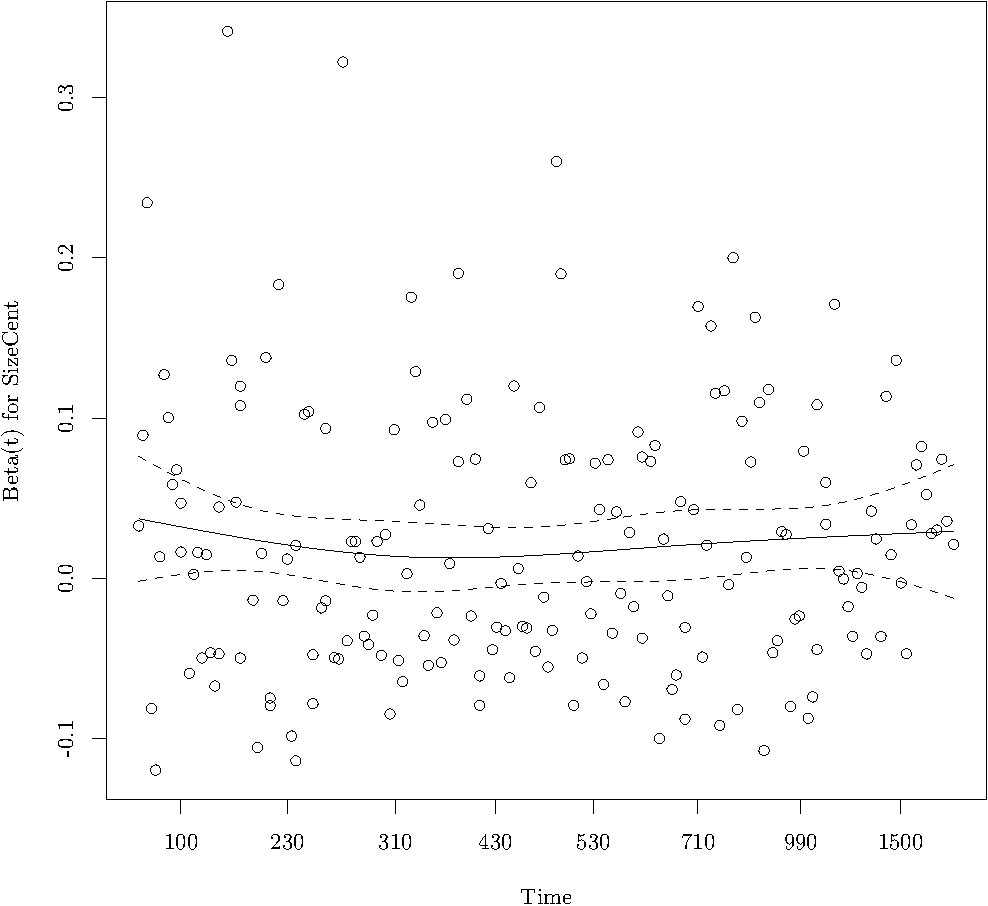
\includegraphics[width=\maxwidth]{figure/05-eda-ph-check-reduced-2-1} 

}




{\centering 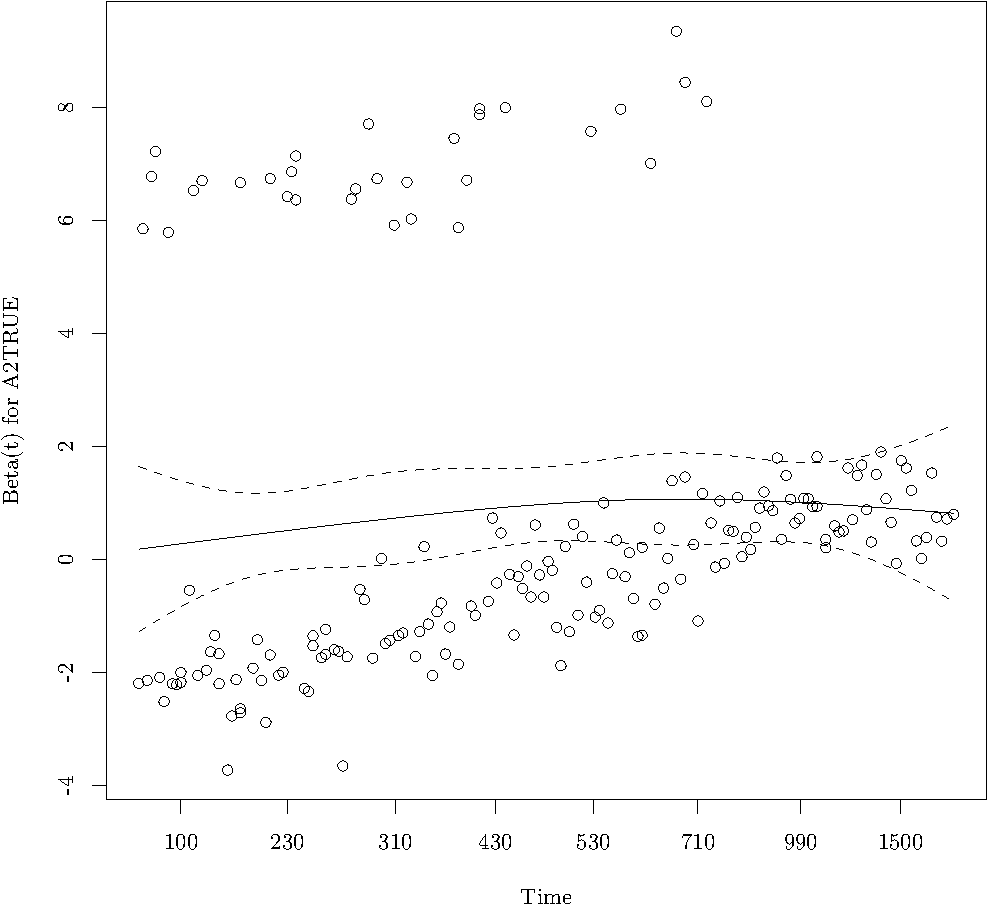
\includegraphics[width=\maxwidth]{figure/05-eda-ph-check-reduced-2-2} 

}




{\centering 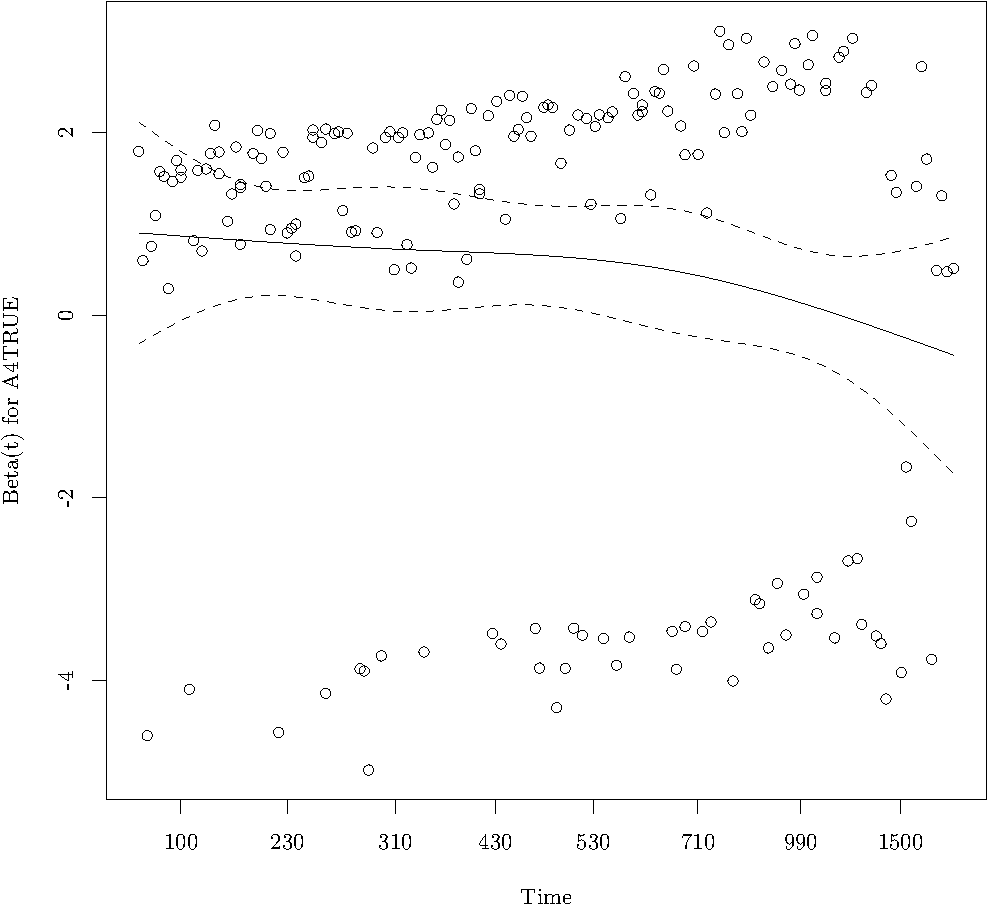
\includegraphics[width=\maxwidth]{figure/05-eda-ph-check-reduced-2-3} 

}



\end{knitrout}


\subsection{Outliers: reduced model}
\begin{knitrout}
\definecolor{shadecolor}{rgb}{0.969, 0.969, 0.969}\color{fgcolor}\begin{kframe}
\begin{alltt}
\hlkwd{scatter.smooth}\hlstd{(}\hlkwd{resid}\hlstd{(fit.cph,} \hlkwc{type} \hlstd{=} \hlstr{"deviance"}\hlstd{), data}\hlopt{$}\hlstd{SizeCent,} \hlkwc{xlab} \hlstd{=} \hlstr{"SizeCent"}\hlstd{,} \hlkwc{main} \hlstd{=} \hlstr{"Deviance vs SizeCent"}\hlstd{,} \hlkwc{ylab} \hlstd{=} \hlstr{"Deviance residuals"}\hlstd{)}
\end{alltt}
\end{kframe}

{\centering 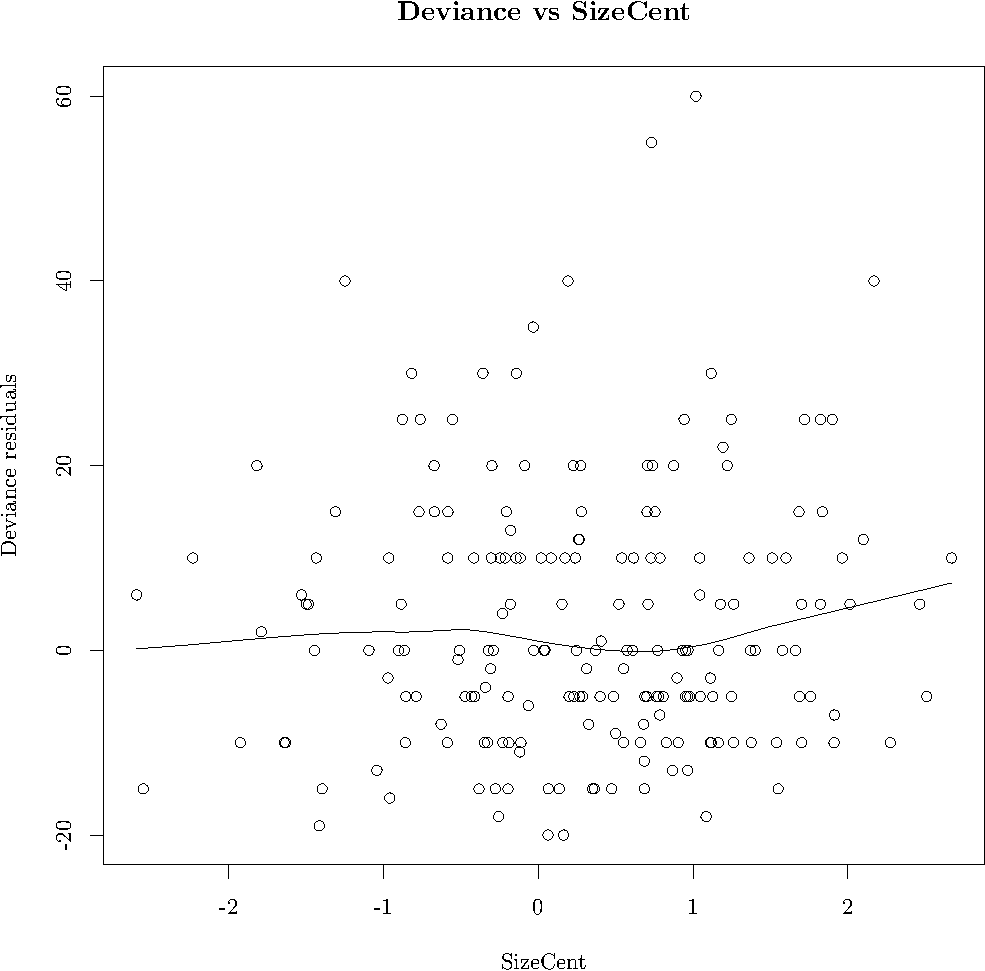
\includegraphics[width=\maxwidth]{figure/05-eda-outliers-reduced-2-1} 

}


\begin{kframe}\begin{alltt}
\hlkwd{boxplot}\hlstd{(}\hlkwd{resid}\hlstd{(fit.cph,} \hlkwc{type} \hlstd{=} \hlstr{"deviance"}\hlstd{)} \hlopt{~} \hlstd{data}\hlopt{$}\hlstd{A2,} \hlkwc{main} \hlstd{=} \hlstr{"Deviance vs A2"}\hlstd{,} \hlkwc{xlab} \hlstd{=} \hlstr{"A2"}\hlstd{,} \hlkwc{ylab} \hlstd{=} \hlstr{"Deviance residuals"}\hlstd{)}
\end{alltt}
\end{kframe}

{\centering 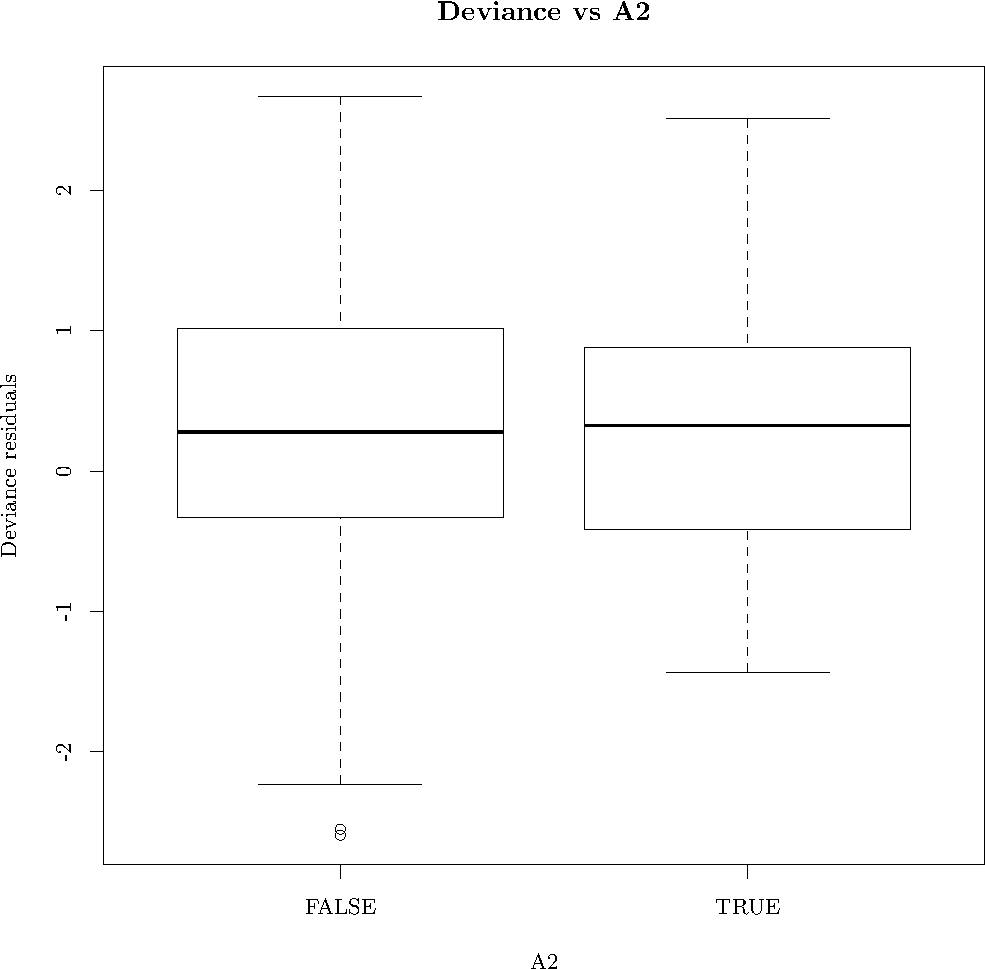
\includegraphics[width=\maxwidth]{figure/05-eda-outliers-reduced-2-2} 

}


\begin{kframe}\begin{alltt}
\hlkwd{boxplot}\hlstd{(}\hlkwd{resid}\hlstd{(fit.cph,} \hlkwc{type} \hlstd{=} \hlstr{"deviance"}\hlstd{)} \hlopt{~} \hlstd{data}\hlopt{$}\hlstd{A4,} \hlkwc{main} \hlstd{=} \hlstr{"Deviance vs A4"}\hlstd{,} \hlkwc{xlab} \hlstd{=} \hlstr{"A4"}\hlstd{,} \hlkwc{ylab} \hlstd{=} \hlstr{"Deviance residuals"}\hlstd{)}
\end{alltt}
\end{kframe}

{\centering 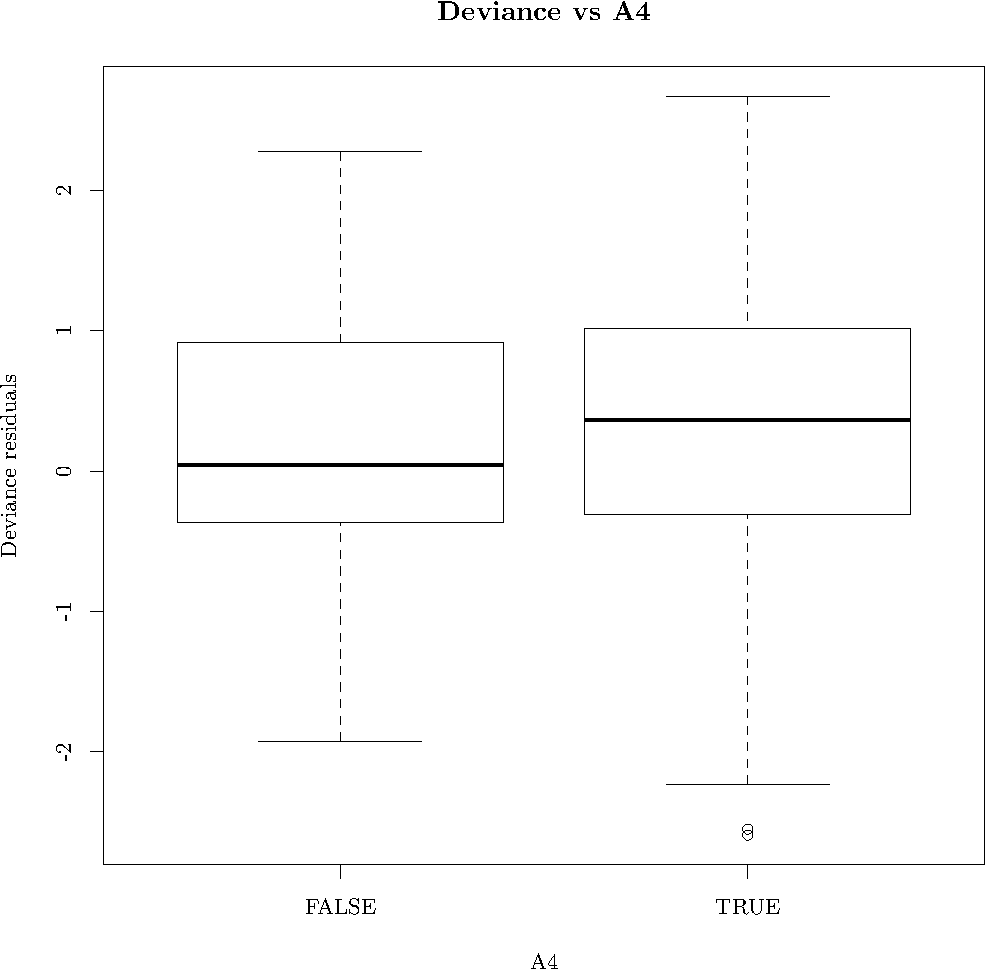
\includegraphics[width=\maxwidth]{figure/05-eda-outliers-reduced-2-3} 

}


\begin{kframe}\begin{alltt}
\hlkwd{plot}\hlstd{(}\hlkwd{resid}\hlstd{(fit.cph,} \hlkwc{type} \hlstd{=} \hlstr{"deviance"}\hlstd{))}
\hlkwd{abline}\hlstd{(}\hlkwc{h} \hlstd{=} \hlkwd{c}\hlstd{(}\hlopt{-}\hlnum{2.5}\hlstd{,} \hlnum{2.5}\hlstd{))}
\end{alltt}
\end{kframe}

{\centering 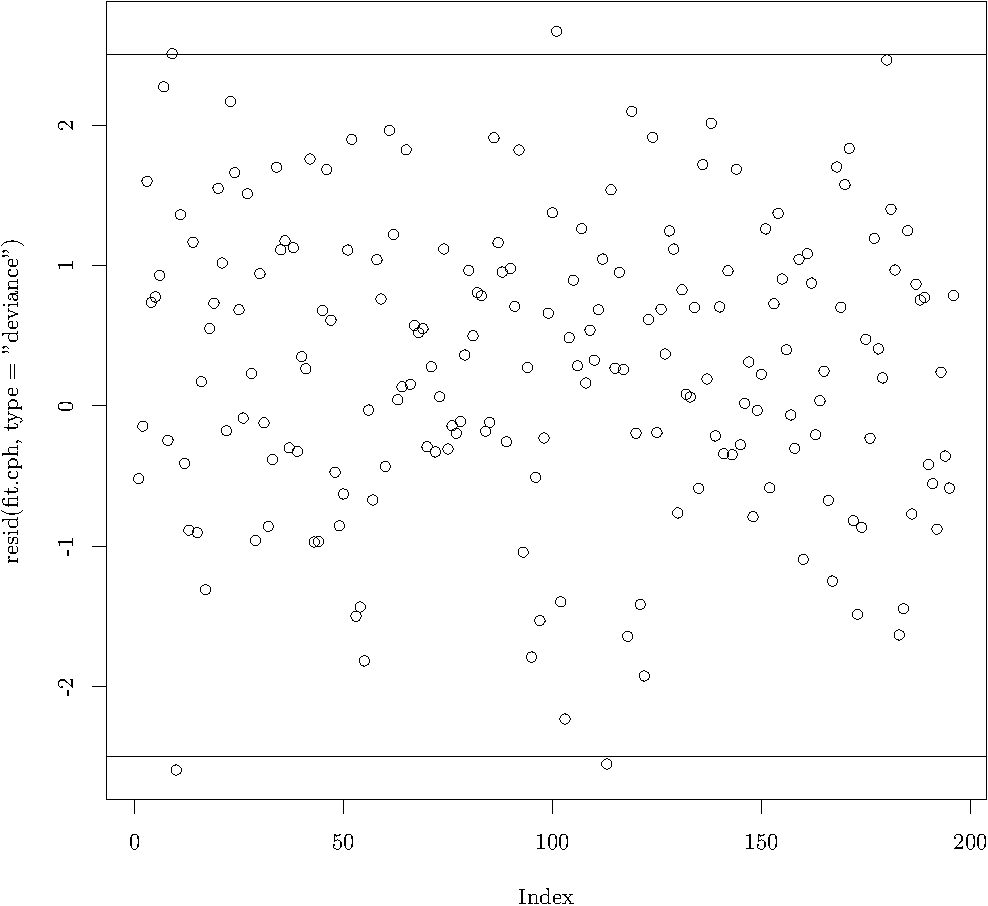
\includegraphics[width=\maxwidth]{figure/05-eda-outliers-reduced-2-4} 

}


\begin{kframe}\begin{alltt}
\hlstd{data}\hlopt{$}\hlstd{devresid} \hlkwb{=} \hlkwd{resid}\hlstd{(fit.cph,} \hlkwc{type} \hlstd{=} \hlstr{"deviance"}\hlstd{)}
\hlstd{temp} \hlkwb{=} \hlstd{data[}\hlkwd{abs}\hlstd{(data}\hlopt{$}\hlstd{devresid)} \hlopt{>=} \hlnum{2.5}\hlstd{,]}
\hlstd{temp[}\hlkwd{order}\hlstd{(temp}\hlopt{$}\hlstd{Time),]}
\end{alltt}
\begin{verbatim}
##            Time   DSD  SexM AgeCent LocBody SizeCent    A2   A4 AgePlus
## NSWPCN_651   20  TRUE  TRUE       8    TRUE       10 FALSE TRUE       3
## NSWPCN_131   61  TRUE FALSE     -11    TRUE       -5  TRUE TRUE       0
## NSWPCN_133 1304 FALSE  TRUE       5   FALSE        6 FALSE TRUE       0
## NSWPCN_667 2415 FALSE FALSE     -14   FALSE      -15 FALSE TRUE       0
##            SizePlus devresid DFBETAS_max
## NSWPCN_651       10    2.669     0.06561
## NSWPCN_131        0    2.510     0.13588
## NSWPCN_133        6   -2.593     0.08199
## NSWPCN_667        0   -2.550     0.19540
\end{verbatim}
\end{kframe}
\end{knitrout}
Few enough that I'm not particularly concerned.  The DFBETAS will be more telling.

\begin{knitrout}
\definecolor{shadecolor}{rgb}{0.969, 0.969, 0.969}\color{fgcolor}\begin{kframe}
\begin{alltt}
\hlstd{temp} \hlkwb{=} \hlkwd{resid}\hlstd{(fit.cph,} \hlkwc{type} \hlstd{=} \hlstr{"dfbetas"}\hlstd{)}
\hlkwd{colnames}\hlstd{(temp)} \hlkwb{=} \hlkwd{names}\hlstd{(fit.cph}\hlopt{$}\hlstd{coefficients)}
\hlstd{temp} \hlkwb{=} \hlkwd{melt}\hlstd{(temp)}
\hlkwd{colnames}\hlstd{(temp)} \hlkwb{=} \hlkwd{c}\hlstd{(}\hlstr{"Patient"}\hlstd{,} \hlstr{"Coefficient"}\hlstd{,} \hlstr{"dfbetas"}\hlstd{)}
\hlstd{temp}\hlopt{$}\hlstd{Patient} \hlkwb{=} \hlkwd{gsub}\hlstd{(}\hlstr{"NSWPCN_"}\hlstd{,} \hlstr{""}\hlstd{, temp}\hlopt{$}\hlstd{Patient)}
\hlnum{2}\hlopt{/}\hlkwd{sqrt}\hlstd{(}\hlkwd{nrow}\hlstd{(data))}      \hlcom{# The classic threshold for concern is 2/sqrt(n).}
\end{alltt}
\begin{verbatim}
## [1] 0.1429
\end{verbatim}
\begin{alltt}
\hlkwd{ggplot}\hlstd{(temp,} \hlkwd{aes}\hlstd{(}\hlkwc{y} \hlstd{=} \hlkwd{abs}\hlstd{(dfbetas),} \hlkwc{x} \hlstd{= Patient,} \hlkwc{col} \hlstd{= Coefficient))} \hlopt{+} \hlkwd{geom_point}\hlstd{()} \hlopt{+} \hlkwd{geom_hline}\hlstd{(}\hlkwc{yintercept} \hlstd{=} \hlnum{2}\hlopt{/}\hlkwd{sqrt}\hlstd{(}\hlkwd{nrow}\hlstd{(data)))}
\end{alltt}
\end{kframe}

{\centering 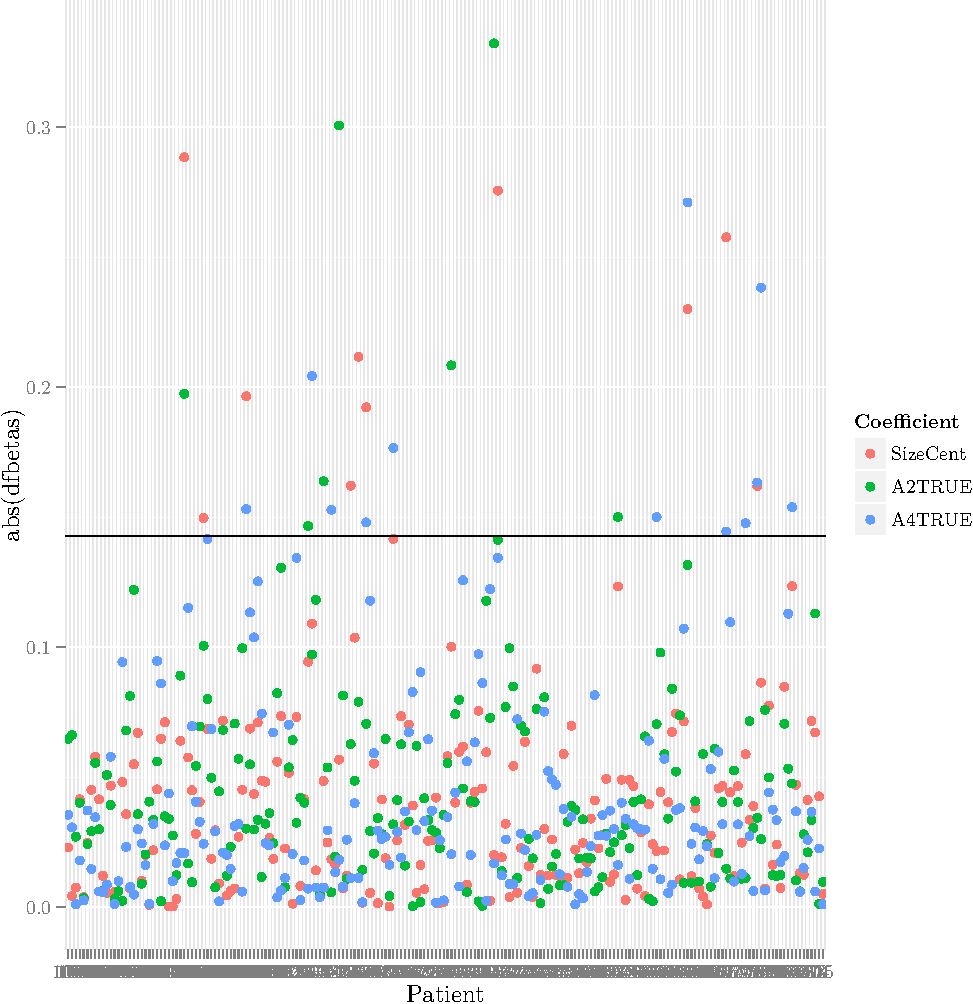
\includegraphics[width=\maxwidth]{figure/05-eda-dfbetas-reduced-2-1} 

}


\begin{kframe}\begin{alltt}
\hlkwd{sort}\hlstd{(}\hlkwd{apply}\hlstd{(}\hlkwd{abs}\hlstd{(}\hlkwd{resid}\hlstd{(fit.cph,} \hlkwc{type} \hlstd{=} \hlstr{"dfbetas"}\hlstd{)),} \hlnum{1}\hlstd{, max),} \hlkwc{decreasing} \hlstd{=} \hlnum{TRUE}\hlstd{)}
\end{alltt}
\begin{verbatim}
##  NSWPCN_317  NSWPCN_145 NSWPCN_1155  NSWPCN_318  NSWPCN_655  NSWPCN_667 
##    0.332189    0.300616    0.288401    0.275569    0.271019    0.257602 
##  NSWPCN_788  NSWPCN_154  NSWPCN_296  NSWPCN_133 NSWPCN_1182  NSWPCN_159 
##    0.238237    0.211651    0.208340    0.204306    0.196498    0.192234 
##  NSWPCN_195  NSWPCN_138  NSWPCN_784  NSWPCN_150  NSWPCN_802  NSWPCN_142 
##    0.176601    0.163765    0.163336    0.162094    0.153829    0.152819 
##  NSWPCN_374  NSWPCN_639 NSWPCN_1167  NSWPCN_777  NSWPCN_131 NSWPCN_1168 
##    0.150036    0.149980    0.149698    0.147613    0.146578    0.141539 
##  NSWPCN_125 NSWPCN_1213  NSWPCN_307 NSWPCN_1188  NSWPCN_316 NSWPCN_1083 
##    0.134329    0.130502    0.125716    0.125290    0.122312    0.122024 
##  NSWPCN_135  NSWPCN_163  NSWPCN_315 NSWPCN_1156 NSWPCN_1186  NSWPCN_814 
##    0.118191    0.117850    0.117799    0.115109    0.113383    0.112947 
##  NSWPCN_801  NSWPCN_674  NSWPCN_654 NSWPCN_1187  NSWPCN_152  NSWPCN_321 
##    0.112912    0.109616    0.107101    0.103757    0.103666    0.099582 
## NSWPCN_1179  NSWPCN_640  NSWPCN_311 NSWPCN_1143 NSWPCN_1072  NSWPCN_333 
##    0.099561    0.097913    0.097227    0.094660    0.094222    0.091738 
##  NSWPCN_269 NSWPCN_1153  NSWPCN_312 NSWPCN_1145  NSWPCN_322  NSWPCN_798 
##    0.090346    0.089045    0.086195    0.085996    0.084851    0.084784 
##  NSWPCN_647  NSWPCN_267 NSWPCN_1207  NSWPCN_364 NSWPCN_1453 NSWPCN_1082 
##    0.083976    0.082720    0.082289    0.081549    0.081363    0.081218 
##  NSWPCN_335  NSWPCN_305  NSWPCN_790  NSWPCN_320  NSWPCN_789 NSWPCN_1189 
##    0.080696    0.079733    0.077517    0.076977    0.075852    0.074420 
##  NSWPCN_648  NSWPCN_304  NSWPCN_651  NSWPCN_200  NSWPCN_323 NSWPCN_1172 
##    0.074397    0.074231    0.073769    0.073425    0.072254    0.071668 
##  NSWPCN_813  NSWPCN_779 NSWPCN_1146 NSWPCN_1177  NSWPCN_257 NSWPCN_1222 
##    0.071557    0.071444    0.071121    0.070598    0.070186    0.070171 
##  NSWPCN_324  NSWPCN_351 NSWPCN_1157 NSWPCN_1165 NSWPCN_1169 NSWPCN_1075 
##    0.069903    0.069788    0.069587    0.069470    0.068473    0.067945 
##  NSWPCN_326 NSWPCN_1198 NSWPCN_1089 NSWPCN_1017  NSWPCN_445   NSWPCN_10 
##    0.067556    0.067186    0.067040    0.066158    0.065687    0.064732 
##  NSWPCN_182  NSWPCN_272 NSWPCN_1227  NSWPCN_636  NSWPCN_310  NSWPCN_268 
##    0.064633    0.064542    0.064241    0.063992    0.063360    0.062023 
##  NSWPCN_664  NSWPCN_665  NSWPCN_164  NSWPCN_348  NSWPCN_661  NSWPCN_643 
##    0.060897    0.059786    0.059209    0.058913    0.058882    0.058810 
##  NSWPCN_294 NSWPCN_1029 NSWPCN_1023 NSWPCN_1178  NSWPCN_308 NSWPCN_1160 
##    0.057991    0.057849    0.057788    0.057040    0.056053    0.054276 
##  NSWPCN_141  NSWPCN_663  NSWPCN_769  NSWPCN_336 NSWPCN_1028  NSWPCN_370 
##    0.053705    0.053123    0.052529    0.052322    0.050802    0.049322 
##  NSWPCN_341  NSWPCN_375  NSWPCN_377 NSWPCN_1190  NSWPCN_344  NSWPCN_804 
##    0.049121    0.048999    0.048868    0.048249    0.047066    0.047059 
##  NSWPCN_666  NSWPCN_381  NSWPCN_770 NSWPCN_1022 NSWPCN_1171 NSWPCN_1148 
##    0.046671    0.046532    0.046523    0.045094    0.044548    0.043732 
##  NSWPCN_815  NSWPCN_280  NSWPCN_126  NSWPCN_270   NSWPCN_13 NSWPCN_1026 
##    0.042601    0.042103    0.042094    0.041841    0.041485    0.041476 
## NSWPCN_1019    NSWPCN_4   NSWPCN_17  NSWPCN_810   NSWPCN_20  NSWPCN_309 
##    0.041459    0.041444    0.041404    0.041224    0.041183    0.040722 
##  NSWPCN_657 NSWPCN_1140  NSWPCN_646  NSWPCN_781  NSWPCN_793  NSWPCN_352 
##    0.040676    0.040590    0.040352    0.038840    0.037494    0.037345 
## NSWPCN_1021  NSWPCN_372  NSWPCN_273  NSWPCN_256 NSWPCN_1193  NSWPCN_284 
##    0.037163    0.037127    0.037070    0.036792    0.036136    0.035452 
##  NSWPCN_369  NSWPCN_166  NSWPCN_363  NSWPCN_376  NSWPCN_358 NSWPCN_1141 
##    0.035357    0.034278    0.034044    0.034002    0.033739    0.033556 
##  NSWPCN_796  NSWPCN_350  NSWPCN_384  NSWPCN_373 NSWPCN_1170  NSWPCN_807 
##    0.033436    0.032884    0.030333    0.030047    0.029544    0.028008 
## NSWPCN_1150  NSWPCN_366 NSWPCN_1018  NSWPCN_330  NSWPCN_149  NSWPCN_283 
##    0.027565    0.027539    0.027076    0.026279    0.025914    0.025793 
##  NSWPCN_775 NSWPCN_1091  NSWPCN_656  NSWPCN_662  NSWPCN_638 NSWPCN_1176 
##    0.024801    0.024454    0.024387    0.024249    0.024214    0.023162 
## NSWPCN_1215 NSWPCN_1139 NSWPCN_1175  NSWPCN_143  NSWPCN_319  NSWPCN_360 
##    0.022560    0.020274    0.020064    0.019477    0.019173    0.019022 
##  NSWPCN_332  NSWPCN_353  NSWPCN_658  NSWPCN_797 NSWPCN_1152  NSWPCN_190 
##    0.018748    0.018719    0.018368    0.017403    0.016949    0.016279 
##  NSWPCN_157  NSWPCN_806  NSWPCN_345  NSWPCN_334 NSWPCN_1027 NSWPCN_1070 
##    0.014358    0.013072    0.012628    0.012443    0.012044    0.009948 
##    NSWPCN_9  NSWPCN_136 NSWPCN_1031 NSWPCN_1020 
##    0.009717    0.005929    0.005825    0.003856
\end{verbatim}
\begin{alltt}
\hlkwd{sum}\hlstd{(}\hlkwd{apply}\hlstd{(}\hlkwd{abs}\hlstd{(}\hlkwd{resid}\hlstd{(fit.cph,} \hlkwc{type} \hlstd{=} \hlstr{"dfbetas"}\hlstd{)),} \hlnum{1}\hlstd{, max)} \hlopt{>} \hlnum{2}\hlopt{/}\hlkwd{sqrt}\hlstd{(}\hlkwd{nrow}\hlstd{(data)))}
\end{alltt}
\begin{verbatim}
## [1] 23
\end{verbatim}
\begin{alltt}
\hlstd{data}\hlopt{$}\hlstd{DFBETAS_max} \hlkwb{=} \hlkwd{apply}\hlstd{(}\hlkwd{abs}\hlstd{(}\hlkwd{resid}\hlstd{(fit.cph,} \hlkwc{type} \hlstd{=} \hlstr{"dfbetas"}\hlstd{)),} \hlnum{1}\hlstd{, max)}
\hlstd{temp} \hlkwb{=} \hlstd{data[data}\hlopt{$}\hlstd{DFBETAS_max} \hlopt{>=} \hlnum{2}\hlopt{/}\hlkwd{sqrt}\hlstd{(}\hlkwd{nrow}\hlstd{(data))} \hlopt{|} \hlkwd{abs}\hlstd{(data}\hlopt{$}\hlstd{devresid)} \hlopt{>=} \hlnum{2.5}\hlstd{,]}
\hlstd{temp[}\hlkwd{order}\hlstd{(temp}\hlopt{$}\hlstd{DFBETAS_max),]}
\end{alltt}
\begin{verbatim}
##             Time   DSD  SexM AgeCent LocBody SizeCent    A2    A4 AgePlus
## NSWPCN_651    20  TRUE  TRUE       8    TRUE       10 FALSE  TRUE       3
## NSWPCN_131    61  TRUE FALSE     -11    TRUE       -5  TRUE  TRUE       0
## NSWPCN_777  1197 FALSE  TRUE      -8   FALSE      -10 FALSE FALSE       0
## NSWPCN_1167  711  TRUE FALSE       1   FALSE       30 FALSE  TRUE       0
## NSWPCN_639  1990  TRUE FALSE       1   FALSE        2 FALSE  TRUE       0
## NSWPCN_374    63  TRUE  TRUE       5   FALSE      -10  TRUE  TRUE       0
## NSWPCN_142  1691  TRUE  TRUE       4   FALSE        0 FALSE FALSE       0
## NSWPCN_802  1072  TRUE FALSE     -14    TRUE       25 FALSE FALSE       0
## NSWPCN_150   270  TRUE  TRUE       6    TRUE       55 FALSE  TRUE       1
## NSWPCN_784  2701  TRUE  TRUE      14   FALSE      -19 FALSE FALSE       9
## NSWPCN_138   559  TRUE FALSE      -6   FALSE        5  TRUE  TRUE       0
## NSWPCN_195  1969  TRUE  TRUE       8   FALSE      -16 FALSE FALSE       3
## NSWPCN_159    30  TRUE  TRUE      11    TRUE       40 FALSE FALSE       6
## NSWPCN_1182 2178  TRUE FALSE      -4    TRUE      -10 FALSE  TRUE       0
## NSWPCN_133  1304 FALSE  TRUE       5   FALSE        6 FALSE  TRUE       0
## NSWPCN_296   671  TRUE  TRUE       2   FALSE       -3  TRUE  TRUE       0
## NSWPCN_154   163  TRUE  TRUE      -2    TRUE       60 FALSE  TRUE       0
## NSWPCN_788  2155 FALSE FALSE       5   FALSE      -10 FALSE FALSE       0
## NSWPCN_667  2415 FALSE FALSE     -14   FALSE      -15 FALSE  TRUE       0
## NSWPCN_655  1723  TRUE  TRUE      11    TRUE       10 FALSE  TRUE       6
## NSWPCN_318  1464  TRUE FALSE       2   FALSE       20 FALSE  TRUE       0
## NSWPCN_1155  390  TRUE FALSE       9    TRUE       40  TRUE  TRUE       4
## NSWPCN_145   599  TRUE  TRUE      -6    TRUE       15  TRUE  TRUE       0
## NSWPCN_317   729  TRUE FALSE      11   FALSE       10  TRUE  TRUE       6
##             SizePlus devresid DFBETAS_max
## NSWPCN_651        10   2.6694     0.07377
## NSWPCN_131         0   2.5095     0.14658
## NSWPCN_777         0  -1.6399     0.14761
## NSWPCN_1167       30  -0.8175     0.14970
## NSWPCN_639         2  -1.7880     0.14998
## NSWPCN_374         0   1.9109     0.15004
## NSWPCN_142         0  -0.9020     0.15282
## NSWPCN_802        25  -0.7615     0.15383
## NSWPCN_150        55   0.7320     0.16209
## NSWPCN_784         0  -1.4137     0.16334
## NSWPCN_138         5  -0.8845     0.16376
## NSWPCN_195         0  -0.9580     0.17660
## NSWPCN_159        40   2.1684     0.19223
## NSWPCN_1182        0  -1.6308     0.19650
## NSWPCN_133         6  -2.5931     0.20431
## NSWPCN_296         0  -0.9693     0.20834
## NSWPCN_154        60   1.0185     0.21165
## NSWPCN_788         0  -1.9230     0.23824
## NSWPCN_667         0  -2.5504     0.25760
## NSWPCN_655        10  -2.2303     0.27102
## NSWPCN_318        20  -1.8160     0.27557
## NSWPCN_1155       40  -1.2469     0.28840
## NSWPCN_145        15  -1.3089     0.30062
## NSWPCN_317        10  -1.4321     0.33219
\end{verbatim}
\end{kframe}
\end{knitrout}





\subsection{Summary of EDA}
\begin{enumerate}
\item On the basis of pre-operative assessability and data availability, variables were filtered down to Sex, AgeCent, LocBody, SizeCent, A2, A4.
\item Functional forms for the continuous variates AgeCent and SizeCent indicated a possible slight quadratic effect on AgeCent, and a knee on SizeCent.  These were modelled by incorporating additional terms.
\item Analysis of a full model fit (with additional nonlinear terms included) indicated violation of PH for gender.  This was dealt with by stratification.  A slight PH violation by age was deemed unimportant. 
\item Variable selection by BIC (both stepwise and genetic all-subset) settled on a final model of Surv(Time,DSD) $\sim$ 1 + strata(SexM) + SizeCent + A2 + A4.  This model was refit by coxph. 
\item PH was verified on the final model.  Deviance residuals showed no egregious outliers. dfBetaS indicated a number of influential observations, which require checking.
\end{enumerate}

\section{Final fits}
\begin{knitrout}
\definecolor{shadecolor}{rgb}{0.969, 0.969, 0.969}\color{fgcolor}\begin{kframe}
\begin{alltt}
\hlstd{fit.cph} \hlkwb{=} \hlkwd{coxph}\hlstd{(}\hlkwd{Surv}\hlstd{(Time, DSD)} \hlopt{~} \hlkwd{strata}\hlstd{(SexM)} \hlopt{+} \hlstd{SizeCent} \hlopt{+} \hlstd{A2} \hlopt{+} \hlstd{A4,} \hlkwc{data} \hlstd{= data)}
\end{alltt}
\end{kframe}
\end{knitrout}

\begin{knitrout}
\definecolor{shadecolor}{rgb}{0.969, 0.969, 0.969}\color{fgcolor}\begin{kframe}
\begin{alltt}
\hlkwd{set.seed}\hlstd{(}\hlnum{20150111}\hlstd{)}
\hlstd{fit.rsf} \hlkwb{=} \hlkwd{rfsrc}\hlstd{(}\hlkwd{Surv}\hlstd{(Time, DSD)} \hlopt{~} \hlstd{SexM} \hlopt{+} \hlstd{AgeCent} \hlopt{+} \hlstd{LocBody} \hlopt{+} \hlstd{SizeCent} \hlopt{+} \hlstd{A2} \hlopt{+} \hlstd{A4,} \hlkwc{data} \hlstd{= data,} \hlkwc{mtry} \hlstd{=} \hlnum{1}\hlstd{,} \hlkwc{splitrule} \hlstd{=} \hlstr{"logrankscore"}\hlstd{,} \hlkwc{nsplit} \hlstd{=} \hlnum{2}\hlstd{,} \hlkwc{ntree} \hlstd{=} \hlnum{1000}\hlstd{)}
\end{alltt}
\end{kframe}
\end{knitrout}

\begin{knitrout}
\definecolor{shadecolor}{rgb}{0.969, 0.969, 0.969}\color{fgcolor}\begin{kframe}
\begin{alltt}
\hlstd{fit.gg} \hlkwb{=} \hlkwd{flexsurvreg}\hlstd{(}\hlkwd{Surv}\hlstd{(Time, DSD)} \hlopt{~} \hlstd{SexM} \hlopt{+} \hlstd{SizeCent} \hlopt{+} \hlstd{A2} \hlopt{+} \hlstd{A4,}
        \hlkwc{anc} \hlstd{=} \hlkwd{list}\hlstd{(}
                \hlkwc{sigma} \hlstd{=} \hlopt{~} \hlstd{SexM,}
                \hlkwc{Q} \hlstd{=} \hlopt{~} \hlstd{SexM),}
        \hlkwc{data} \hlstd{= data,} \hlkwc{dist} \hlstd{=} \hlstr{"gengamma"}\hlstd{)}

\hlstd{fit.gf} \hlkwb{=} \hlkwd{flexsurvreg}\hlstd{(}\hlkwd{Surv}\hlstd{(Time, DSD)} \hlopt{~} \hlstd{SexM} \hlopt{+} \hlstd{SizeCent} \hlopt{+} \hlstd{A2} \hlopt{+} \hlstd{A4,}
        \hlkwc{anc} \hlstd{=} \hlkwd{list}\hlstd{(}
                \hlkwc{sigma} \hlstd{=} \hlopt{~} \hlstd{SexM,}
                \hlkwc{Q} \hlstd{=} \hlopt{~} \hlstd{SexM,}
                \hlkwc{P} \hlstd{=} \hlopt{~} \hlstd{SexM),}
        \hlkwc{data} \hlstd{= data,} \hlkwc{dist} \hlstd{=} \hlstr{"genf"}\hlstd{)}

\hlstd{fit.gg}\hlopt{$}\hlstd{loglik}
\end{alltt}
\begin{verbatim}
## [1] -1355
\end{verbatim}
\begin{alltt}
\hlstd{fit.gf}\hlopt{$}\hlstd{loglik}
\end{alltt}
\begin{verbatim}
## [1] -1354
\end{verbatim}
\begin{alltt}
\hlkwd{pchisq}\hlstd{(}\hlnum{2}\hlopt{*}\hlstd{(fit.gf}\hlopt{$}\hlstd{loglik} \hlopt{-} \hlstd{fit.gg}\hlopt{$}\hlstd{loglik),} \hlnum{2}\hlstd{,} \hlkwc{lower.tail} \hlstd{=} \hlnum{FALSE}\hlstd{)}
\end{alltt}
\begin{verbatim}
## [1] 0.1734
\end{verbatim}
\begin{alltt}
\hlkwd{AIC}\hlstd{(fit.gg)}
\end{alltt}
\begin{verbatim}
## [1] 2729
\end{verbatim}
\begin{alltt}
\hlkwd{AIC}\hlstd{(fit.gf)}
\end{alltt}
\begin{verbatim}
## [1] 2729
\end{verbatim}
\begin{alltt}
\hlkwd{BIC}\hlstd{(fit.gg)}
\end{alltt}
\begin{verbatim}
## [1] 2758
\end{verbatim}
\begin{alltt}
\hlkwd{BIC}\hlstd{(fit.gf)}
\end{alltt}
\begin{verbatim}
## [1] 2765
\end{verbatim}
\begin{alltt}
\hlstd{fit.gg}
\end{alltt}
\begin{verbatim}
## 
## Call:
## flexsurvreg(formula = Surv(Time, DSD) ~ SexM + SizeCent + A2 +     A4, anc = list(sigma = ~SexM, Q = ~SexM), data = data, dist = "gengamma")
## 
## Estimates: 
##                  data mean  est      L95%     U95%     se       exp(est)
## mu                    NA     6.5307   6.2018   6.8597   0.1678       NA 
## sigma                 NA     0.8130   0.7047   0.9380   0.0593       NA 
## Q                     NA     0.0638  -0.5270   0.6546   0.3014       NA 
## SexMTRUE          0.4898     0.3990   0.0642   0.7338   0.1708   1.4903 
## SizeCent          2.8316    -0.0146  -0.0219  -0.0074   0.0037   0.9855 
## A2TRUE            0.1582    -0.5181  -0.7854  -0.2507   0.1364   0.5957 
## A4TRUE            0.7398    -0.3981  -0.6294  -0.1669   0.1180   0.6716 
## sigma(SexMTRUE)   0.4898    -0.3577  -0.5946  -0.1208   0.1209   0.6993 
## Q(SexMTRUE)       0.4898     0.9493   0.2087   1.6898   0.3778   2.5838 
##                  L95%     U95%   
## mu                    NA       NA
## sigma                 NA       NA
## Q                     NA       NA
## SexMTRUE          1.0663   2.0831
## SizeCent          0.9783   0.9926
## A2TRUE            0.4559   0.7782
## A4TRUE            0.5329   0.8463
## sigma(SexMTRUE)   0.5518   0.8862
## Q(SexMTRUE)       1.2321   5.4183
## 
## N = 196,  Events: 187,  Censored: 9
## Total time at risk: 121359
## Log-likelihood = -1355, df = 9
## AIC = 2729
\end{verbatim}
\end{kframe}
\end{knitrout}

\section{Fit assessment}
Plot fit stratified by sex, separate curves for A2, A4 status, at median (approx.) Size.
\begin{knitrout}
\definecolor{shadecolor}{rgb}{0.969, 0.969, 0.969}\color{fgcolor}\begin{kframe}
\begin{alltt}
\hlstd{temp.grid} \hlkwb{=} \hlkwd{expand.grid}\hlstd{(}\hlkwc{A4} \hlstd{=} \hlkwd{c}\hlstd{(}\hlnum{FALSE}\hlstd{,} \hlnum{TRUE}\hlstd{),} \hlkwc{A2} \hlstd{=} \hlkwd{c}\hlstd{(}\hlnum{FALSE}\hlstd{,} \hlnum{TRUE}\hlstd{),} \hlkwc{SexM} \hlstd{=} \hlkwd{c}\hlstd{(}\hlnum{FALSE}\hlstd{,} \hlnum{TRUE}\hlstd{),} \hlkwc{SizeCent} \hlstd{=} \hlnum{0}\hlstd{)}
\hlstd{temp.grid}\hlopt{$}\hlstd{ID} \hlkwb{=} \hlkwd{sprintf}\hlstd{(}\hlstr{"SexM=%s, A2=% -5s, A4=% -5s"}\hlstd{, temp.grid}\hlopt{$}\hlstd{SexM, temp.grid}\hlopt{$}\hlstd{A2, temp.grid}\hlopt{$}\hlstd{A4)}
\hlstd{temp.preds} \hlkwb{=} \hlkwd{summary}\hlstd{(fit.gg,} \hlkwc{newdata} \hlstd{= temp.grid,} \hlkwc{type} \hlstd{=} \hlstr{"survival"}\hlstd{,} \hlkwc{t} \hlstd{=} \hlkwd{seq}\hlstd{(}\hlnum{0}\hlstd{,} \hlnum{365}\hlopt{*}\hlnum{5}\hlstd{,} \hlnum{30}\hlstd{))}
\hlstd{temp.preds2} \hlkwb{=} \hlkwd{do.call}\hlstd{(rbind, temp.preds)}
\hlstd{temp.preds2}\hlopt{$}\hlstd{group} \hlkwb{=} \hlkwd{rep}\hlstd{(}\hlkwd{gsub}\hlstd{(}\hlstr{".*ID="}\hlstd{,} \hlstr{""}\hlstd{,} \hlkwd{names}\hlstd{(temp.preds)),} \hlkwc{each} \hlstd{=} \hlkwd{nrow}\hlstd{(temp.preds[[}\hlnum{1}\hlstd{]]))}
\hlstd{temp.preds.cox} \hlkwb{=} \hlkwd{survfit}\hlstd{(fit.cph,} \hlkwc{newdata} \hlstd{= temp.grid)}

\hlstd{temp.survfit} \hlkwb{=} \hlkwd{survfit}\hlstd{(}\hlkwd{Surv}\hlstd{(Time, DSD)} \hlopt{~} \hlstd{SexM} \hlopt{+} \hlstd{A2} \hlopt{+} \hlstd{A4, data)}
\hlstd{temp.data} \hlkwb{=} \hlkwd{data.frame}\hlstd{(}\hlkwc{time} \hlstd{= temp.survfit}\hlopt{$}\hlstd{time,} \hlkwc{surv} \hlstd{= temp.survfit}\hlopt{$}\hlstd{surv,} \hlkwc{upper} \hlstd{= temp.survfit}\hlopt{$}\hlstd{lower,} \hlkwc{lower} \hlstd{= temp.survfit}\hlopt{$}\hlstd{upper,} \hlkwc{group} \hlstd{=} \hlkwd{rep}\hlstd{(}\hlkwd{names}\hlstd{(temp.survfit}\hlopt{$}\hlstd{strata), temp.survfit}\hlopt{$}\hlstd{strata),} \hlkwc{model} \hlstd{=} \hlstr{"KM"}\hlstd{)}
\hlstd{temp.data} \hlkwb{=} \hlkwd{rbind}\hlstd{(temp.data,} \hlkwd{data.frame}\hlstd{(}\hlkwc{time} \hlstd{= temp.preds2}\hlopt{$}\hlstd{time,} \hlkwc{surv} \hlstd{= temp.preds2}\hlopt{$}\hlstd{est,} \hlkwc{upper} \hlstd{= temp.preds2}\hlopt{$}\hlstd{ucl,} \hlkwc{lower} \hlstd{= temp.preds2}\hlopt{$}\hlstd{lcl,} \hlkwc{group} \hlstd{= temp.preds2}\hlopt{$}\hlstd{group,} \hlkwc{model} \hlstd{=} \hlstr{"GG"}\hlstd{))}
\hlstd{temp.data} \hlkwb{=} \hlkwd{rbind}\hlstd{(temp.data,} \hlkwd{data.frame}\hlstd{(}\hlkwc{time} \hlstd{= temp.preds.cox}\hlopt{$}\hlstd{time,} \hlkwc{surv} \hlstd{= temp.preds.cox}\hlopt{$}\hlstd{surv,} \hlkwc{upper} \hlstd{= temp.preds.cox}\hlopt{$}\hlstd{upper,} \hlkwc{lower} \hlstd{= temp.preds.cox}\hlopt{$}\hlstd{lower,} \hlkwc{group} \hlstd{=} \hlkwd{rep}\hlstd{(temp.grid}\hlopt{$}\hlstd{ID, temp.preds.cox}\hlopt{$}\hlstd{strata),} \hlkwc{model} \hlstd{=} \hlstr{"CPH"}\hlstd{))}

\hlstd{temp.data}\hlopt{$}\hlstd{Sex} \hlkwb{=} \hlkwd{c}\hlstd{(}\hlstr{"Male"}\hlstd{,} \hlstr{"Female"}\hlstd{)[}\hlkwd{grepl}\hlstd{(}\hlstr{"SexM=FALSE"}\hlstd{, temp.data}\hlopt{$}\hlstd{group)}\hlopt{+}\hlnum{1}\hlstd{]}
\hlstd{temp.data}\hlopt{$}\hlstd{A2} \hlkwb{=} \hlkwd{c}\hlstd{(}\hlstr{"A2-"}\hlstd{,} \hlstr{"A2+"}\hlstd{)[}\hlkwd{grepl}\hlstd{(}\hlstr{"A2=TRUE"}\hlstd{, temp.data}\hlopt{$}\hlstd{group)}\hlopt{+}\hlnum{1}\hlstd{]}
\hlstd{temp.data}\hlopt{$}\hlstd{A4} \hlkwb{=} \hlkwd{c}\hlstd{(}\hlstr{"A4-"}\hlstd{,} \hlstr{"A4+"}\hlstd{)[}\hlkwd{grepl}\hlstd{(}\hlstr{"A4=TRUE"}\hlstd{, temp.data}\hlopt{$}\hlstd{group)}\hlopt{+}\hlnum{1}\hlstd{]}

\hlkwd{ggplot}\hlstd{(temp.data,} \hlkwd{aes}\hlstd{(}\hlkwc{x} \hlstd{=} \hlkwd{log}\hlstd{(time),} \hlkwc{y} \hlstd{=} \hlkwd{log}\hlstd{(}\hlopt{-}\hlkwd{log}\hlstd{(surv)),} \hlkwc{ymin} \hlstd{=} \hlkwd{log}\hlstd{(}\hlopt{-}\hlkwd{log}\hlstd{(lower)),} \hlkwc{ymax} \hlstd{=} \hlkwd{log}\hlstd{(}\hlopt{-}\hlkwd{log}\hlstd{(upper)),} \hlkwc{colour} \hlstd{= model,} \hlkwc{fill} \hlstd{= model))} \hlopt{+}
        \hlkwd{geom_ribbon}\hlstd{(}\hlkwc{alpha} \hlstd{=} \hlnum{0.25}\hlstd{,} \hlkwc{colour} \hlstd{=} \hlnum{NA}\hlstd{)} \hlopt{+}
        \hlkwd{geom_line}\hlstd{()} \hlopt{+}
        \hlkwd{xlim}\hlstd{(}\hlnum{4}\hlstd{,} \hlnum{7}\hlstd{)} \hlopt{+} \hlkwd{ylim}\hlstd{(}\hlopt{-}\hlnum{4}\hlstd{,} \hlnum{2}\hlstd{)} \hlopt{+}
        \hlkwd{facet_grid}\hlstd{(A2} \hlopt{~} \hlstd{A4} \hlopt{~} \hlstd{Sex)}
\end{alltt}


{\ttfamily\noindent\color{warningcolor}{\#\# Warning: Removed 50 rows containing missing values (geom\_path).}}

{\ttfamily\noindent\color{warningcolor}{\#\# Warning: Removed 45 rows containing missing values (geom\_path).}}

{\ttfamily\noindent\color{warningcolor}{\#\# Warning: Removed 51 rows containing missing values (geom\_path).}}

{\ttfamily\noindent\color{warningcolor}{\#\# Warning: Removed 43 rows containing missing values (geom\_path).}}

{\ttfamily\noindent\color{warningcolor}{\#\# Warning: Removed 41 rows containing missing values (geom\_path).}}

{\ttfamily\noindent\color{warningcolor}{\#\# Warning: Removed 38 rows containing missing values (geom\_path).}}

{\ttfamily\noindent\color{warningcolor}{\#\# Warning: Removed 41 rows containing missing values (geom\_path).}}

{\ttfamily\noindent\color{warningcolor}{\#\# Warning: Removed 39 rows containing missing values (geom\_path).}}\end{kframe}

{\centering 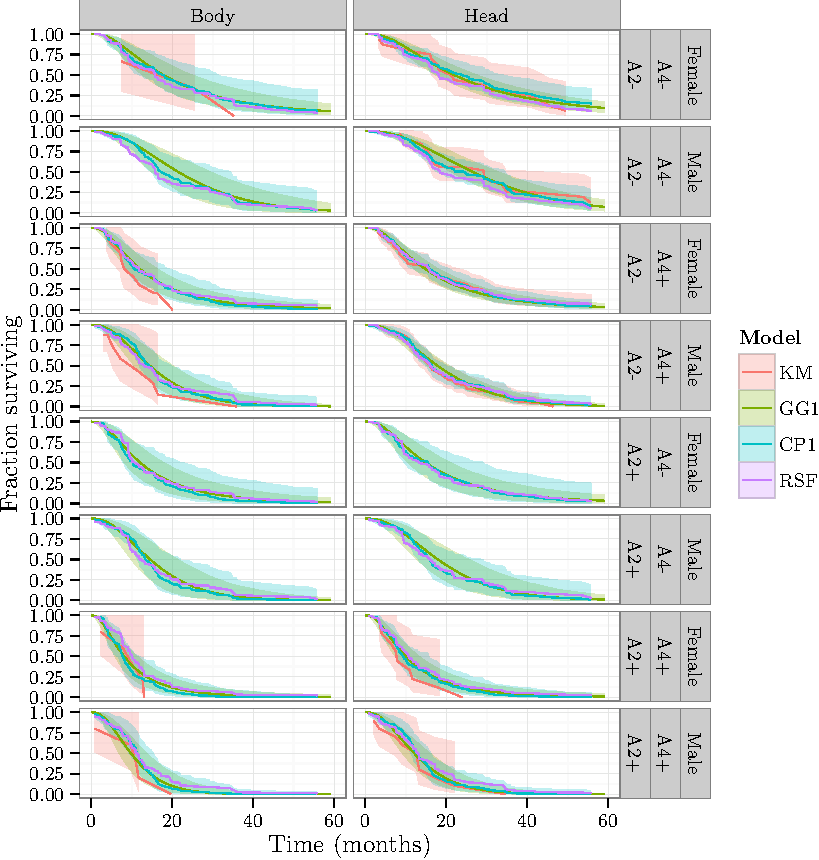
\includegraphics[width=\maxwidth]{figure/05-final-fit-assessment-1} 

}


\begin{kframe}\begin{alltt}
\hlkwd{ggplot}\hlstd{(temp.data,} \hlkwd{aes}\hlstd{(}\hlkwc{x} \hlstd{= time,} \hlkwc{y} \hlstd{= surv,} \hlkwc{ymin} \hlstd{= lower,} \hlkwc{ymax} \hlstd{= upper,} \hlkwc{colour} \hlstd{= model,} \hlkwc{fill} \hlstd{= model))} \hlopt{+}
        \hlkwd{geom_ribbon}\hlstd{(}\hlkwc{alpha} \hlstd{=} \hlnum{0.25}\hlstd{,} \hlkwc{colour} \hlstd{=} \hlnum{NA}\hlstd{)} \hlopt{+}
        \hlkwd{geom_line}\hlstd{()} \hlopt{+} \hlkwd{xlim}\hlstd{(}\hlnum{0}\hlstd{,} \hlnum{2000}\hlstd{)} \hlopt{+} \hlkwd{ylim}\hlstd{(}\hlnum{0}\hlstd{,} \hlnum{1}\hlstd{)} \hlopt{+}
        \hlkwd{facet_grid}\hlstd{(A2} \hlopt{~} \hlstd{A4} \hlopt{~} \hlstd{Sex)}
\end{alltt}


{\ttfamily\noindent\color{warningcolor}{\#\# Warning: Removed 4 rows containing missing values (geom\_path).}}

{\ttfamily\noindent\color{warningcolor}{\#\# Warning: Removed 2 rows containing missing values (geom\_path).}}

{\ttfamily\noindent\color{warningcolor}{\#\# Warning: Removed 5 rows containing missing values (geom\_path).}}

{\ttfamily\noindent\color{warningcolor}{\#\# Warning: Removed 1 rows containing missing values (geom\_path).}}

{\ttfamily\noindent\color{warningcolor}{\#\# Warning: Removed 3 rows containing missing values (geom\_path).}}

{\ttfamily\noindent\color{warningcolor}{\#\# Warning: Removed 1 rows containing missing values (geom\_path).}}

{\ttfamily\noindent\color{warningcolor}{\#\# Warning: Removed 3 rows containing missing values (geom\_path).}}

{\ttfamily\noindent\color{warningcolor}{\#\# Warning: Removed 1 rows containing missing values (geom\_path).}}\end{kframe}

{\centering 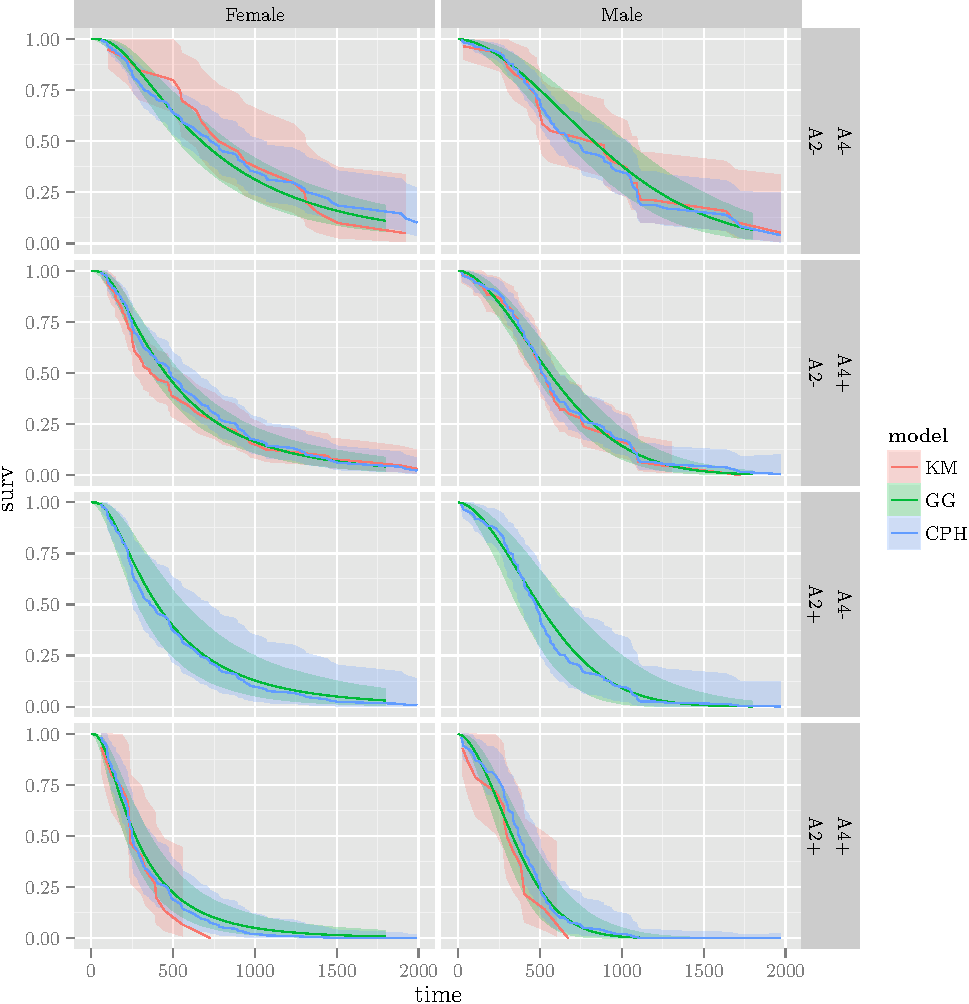
\includegraphics[width=\maxwidth]{figure/05-final-fit-assessment-2} 

}



\end{knitrout}

Some deviation though not significant.  Most concerning is the A2- A4- female group, survival of which is underestimated by the flexsurv model.  To approach this in a modelling sense would require interaction terms between Sex and A2, A4. Overfitting seems likely considering the very few data available for the A2+/A4- group.  Perhaps just add a single "DoubleNegFemale" term.
\begin{knitrout}
\definecolor{shadecolor}{rgb}{0.969, 0.969, 0.969}\color{fgcolor}\begin{kframe}
\begin{alltt}
\hlstd{fit.gg2} \hlkwb{=} \hlkwd{flexsurvreg}\hlstd{(}\hlkwd{Surv}\hlstd{(Time, DSD)} \hlopt{~} \hlstd{SexM} \hlopt{+} \hlstd{SizeCent} \hlopt{+} \hlstd{A2} \hlopt{+} \hlstd{A4} \hlopt{+} \hlkwd{I}\hlstd{(SexM} \hlopt{==} \hlnum{FALSE} \hlopt{&} \hlstd{A2} \hlopt{==} \hlnum{FALSE} \hlopt{&} \hlstd{A4} \hlopt{==} \hlnum{FALSE}\hlstd{),}
        \hlkwc{anc} \hlstd{=} \hlkwd{list}\hlstd{(}
                \hlkwc{sigma} \hlstd{=} \hlopt{~} \hlstd{SexM,}
                \hlkwc{Q} \hlstd{=} \hlopt{~} \hlstd{SexM),}
        \hlkwc{data} \hlstd{= data,} \hlkwc{dist} \hlstd{=} \hlstr{"gengamma"}\hlstd{)}

\hlstd{fit.gg2}
\end{alltt}
\begin{verbatim}
## 
## Call:
## flexsurvreg(formula = Surv(Time, DSD) ~ SexM + SizeCent + A2 +     A4 + I(SexM == FALSE & A2 == FALSE & A4 == FALSE), anc = list(sigma = ~SexM,     Q = ~SexM), data = data, dist = "gengamma")
## 
## Estimates: 
##                                                   data mean  est     
## mu                                                      NA    6.39906
## sigma                                                   NA    0.81027
## Q                                                       NA    0.04270
## SexMTRUE                                           0.48980    0.47352
## SizeCent                                           2.83163   -0.01510
## A2TRUE                                             0.15816   -0.51111
## A4TRUE                                             0.73980   -0.31385
## I(SexM == FALSE & A2 == FALSE & A4 == FALSE)TRUE   0.10204    0.28405
## sigma(SexMTRUE)                                    0.48980   -0.35966
## Q(SexMTRUE)                                        0.48980    0.97670
##                                                   L95%      U95%    
## mu                                                 6.01578   6.78235
## sigma                                              0.70295   0.93397
## Q                                                 -0.51759   0.60298
## SexMTRUE                                           0.12517   0.82188
## SizeCent                                          -0.02230  -0.00789
## A2TRUE                                            -0.78047  -0.24176
## A4TRUE                                            -0.57639  -0.05131
## I(SexM == FALSE & A2 == FALSE & A4 == FALSE)TRUE  -0.19015   0.75824
## sigma(SexMTRUE)                                   -0.59596  -0.12335
## Q(SexMTRUE)                                        0.25579   1.69761
##                                                   se        exp(est)
## mu                                                 0.19556        NA
## sigma                                              0.05874        NA
## Q                                                  0.28587        NA
## SexMTRUE                                           0.17774   1.60564
## SizeCent                                           0.00368   0.98502
## A2TRUE                                             0.13743   0.59983
## A4TRUE                                             0.13395   0.73063
## I(SexM == FALSE & A2 == FALSE & A4 == FALSE)TRUE   0.24194   1.32849
## sigma(SexMTRUE)                                    0.12057   0.69792
## Q(SexMTRUE)                                        0.36782   2.65568
##                                                   L95%      U95%    
## mu                                                      NA        NA
## sigma                                                   NA        NA
## Q                                                       NA        NA
## SexMTRUE                                           1.13334   2.27477
## SizeCent                                           0.97795   0.99214
## A2TRUE                                             0.45819   0.78525
## A4TRUE                                             0.56192   0.94999
## I(SexM == FALSE & A2 == FALSE & A4 == FALSE)TRUE   0.82684   2.13452
## sigma(SexMTRUE)                                    0.55103   0.88395
## Q(SexMTRUE)                                        1.29148   5.46090
## 
## N = 196,  Events: 187,  Censored: 9
## Total time at risk: 121359
## Log-likelihood = -1355, df = 10
## AIC = 2729
\end{verbatim}
\begin{alltt}
\hlkwd{AIC}\hlstd{(fit.gg)}
\end{alltt}
\begin{verbatim}
## [1] 2729
\end{verbatim}
\begin{alltt}
\hlkwd{AIC}\hlstd{(fit.gg2)}
\end{alltt}
\begin{verbatim}
## [1] 2729
\end{verbatim}
\begin{alltt}
\hlkwd{AIC}\hlstd{(fit.gg)} \hlopt{-} \hlkwd{AIC}\hlstd{(fit.gg2)}
\end{alltt}
\begin{verbatim}
## [1] -0.6318
\end{verbatim}
\begin{alltt}
\hlcom{# Equivocal on AIC.  BIC would favour gg then.}

\hlkwd{pchisq}\hlstd{(}\hlopt{-}\hlnum{2}\hlopt{*}\hlstd{(fit.gg}\hlopt{$}\hlstd{loglik} \hlopt{-} \hlstd{fit.gg2}\hlopt{$}\hlstd{loglik),} \hlnum{1}\hlstd{,} \hlkwc{lower.tail} \hlstd{=} \hlnum{FALSE}\hlstd{)}
\end{alltt}
\begin{verbatim}
## [1] 0.2421
\end{verbatim}
\begin{alltt}
\hlcom{# Not good evidence on LRT}
\end{alltt}
\end{kframe}
\end{knitrout}

See how it plots relative to the others.
\begin{knitrout}
\definecolor{shadecolor}{rgb}{0.969, 0.969, 0.969}\color{fgcolor}\begin{kframe}
\begin{alltt}
\hlstd{temp.preds} \hlkwb{=} \hlkwd{summary}\hlstd{(fit.gg2,} \hlkwc{newdata} \hlstd{= temp.grid,} \hlkwc{type} \hlstd{=} \hlstr{"survival"}\hlstd{,} \hlkwc{t} \hlstd{=} \hlkwd{seq}\hlstd{(}\hlnum{0}\hlstd{,} \hlnum{365}\hlopt{*}\hlnum{5}\hlstd{,} \hlnum{30}\hlstd{))}
\hlstd{temp.preds2} \hlkwb{=} \hlkwd{do.call}\hlstd{(rbind, temp.preds)}
\hlstd{temp.preds2}\hlopt{$}\hlstd{group} \hlkwb{=} \hlkwd{rep}\hlstd{(}\hlkwd{gsub}\hlstd{(}\hlstr{".*ID="}\hlstd{,} \hlstr{""}\hlstd{,} \hlkwd{names}\hlstd{(temp.preds)),} \hlkwc{each} \hlstd{=} \hlkwd{nrow}\hlstd{(temp.preds[[}\hlnum{1}\hlstd{]]))}
\hlstd{temp.data} \hlkwb{=} \hlkwd{rbind}\hlstd{(temp.data,} \hlkwd{data.frame}\hlstd{(}\hlkwc{time} \hlstd{= temp.preds2}\hlopt{$}\hlstd{time,} \hlkwc{surv} \hlstd{= temp.preds2}\hlopt{$}\hlstd{est,} \hlkwc{upper} \hlstd{= temp.preds2}\hlopt{$}\hlstd{ucl,} \hlkwc{lower} \hlstd{= temp.preds2}\hlopt{$}\hlstd{lcl,} \hlkwc{group} \hlstd{= temp.preds2}\hlopt{$}\hlstd{group,} \hlkwc{model} \hlstd{=} \hlstr{"GG2"}\hlstd{,} \hlkwc{Sex} \hlstd{=} \hlnum{NA}\hlstd{,} \hlkwc{A2} \hlstd{=} \hlnum{NA}\hlstd{,} \hlkwc{A4} \hlstd{=} \hlnum{NA}\hlstd{))}
\hlstd{temp.data}\hlopt{$}\hlstd{Sex} \hlkwb{=} \hlkwd{c}\hlstd{(}\hlstr{"Male"}\hlstd{,} \hlstr{"Female"}\hlstd{)[}\hlkwd{grepl}\hlstd{(}\hlstr{"SexM=FALSE"}\hlstd{, temp.data}\hlopt{$}\hlstd{group)}\hlopt{+}\hlnum{1}\hlstd{]}
\hlstd{temp.data}\hlopt{$}\hlstd{A2} \hlkwb{=} \hlkwd{c}\hlstd{(}\hlstr{"A2-"}\hlstd{,} \hlstr{"A2+"}\hlstd{)[}\hlkwd{grepl}\hlstd{(}\hlstr{"A2=TRUE"}\hlstd{, temp.data}\hlopt{$}\hlstd{group)}\hlopt{+}\hlnum{1}\hlstd{]}
\hlstd{temp.data}\hlopt{$}\hlstd{A4} \hlkwb{=} \hlkwd{c}\hlstd{(}\hlstr{"A4-"}\hlstd{,} \hlstr{"A4+"}\hlstd{)[}\hlkwd{grepl}\hlstd{(}\hlstr{"A4=TRUE"}\hlstd{, temp.data}\hlopt{$}\hlstd{group)}\hlopt{+}\hlnum{1}\hlstd{]}

\hlkwd{ggplot}\hlstd{(temp.data,} \hlkwd{aes}\hlstd{(}\hlkwc{x} \hlstd{=} \hlkwd{log}\hlstd{(time),} \hlkwc{y} \hlstd{=} \hlkwd{log}\hlstd{(}\hlopt{-}\hlkwd{log}\hlstd{(surv)),} \hlkwc{ymin} \hlstd{=} \hlkwd{log}\hlstd{(}\hlopt{-}\hlkwd{log}\hlstd{(lower)),} \hlkwc{ymax} \hlstd{=} \hlkwd{log}\hlstd{(}\hlopt{-}\hlkwd{log}\hlstd{(upper)),} \hlkwc{colour} \hlstd{= model,} \hlkwc{fill} \hlstd{= model))} \hlopt{+}
        \hlkwd{geom_ribbon}\hlstd{(}\hlkwc{alpha} \hlstd{=} \hlnum{0.25}\hlstd{,} \hlkwc{colour} \hlstd{=} \hlnum{NA}\hlstd{)} \hlopt{+}
        \hlkwd{geom_line}\hlstd{()} \hlopt{+}
        \hlkwd{xlim}\hlstd{(}\hlnum{4}\hlstd{,} \hlnum{7}\hlstd{)} \hlopt{+} \hlkwd{ylim}\hlstd{(}\hlopt{-}\hlnum{4}\hlstd{,} \hlnum{2}\hlstd{)} \hlopt{+}
        \hlkwd{facet_grid}\hlstd{(A2} \hlopt{~} \hlstd{A4} \hlopt{~} \hlstd{Sex)}
\end{alltt}


{\ttfamily\noindent\color{warningcolor}{\#\# Warning: Removed 75 rows containing missing values (geom\_path).}}

{\ttfamily\noindent\color{warningcolor}{\#\# Warning: Removed 70 rows containing missing values (geom\_path).}}

{\ttfamily\noindent\color{warningcolor}{\#\# Warning: Removed 76 rows containing missing values (geom\_path).}}

{\ttfamily\noindent\color{warningcolor}{\#\# Warning: Removed 68 rows containing missing values (geom\_path).}}

{\ttfamily\noindent\color{warningcolor}{\#\# Warning: Removed 66 rows containing missing values (geom\_path).}}

{\ttfamily\noindent\color{warningcolor}{\#\# Warning: Removed 63 rows containing missing values (geom\_path).}}

{\ttfamily\noindent\color{warningcolor}{\#\# Warning: Removed 66 rows containing missing values (geom\_path).}}

{\ttfamily\noindent\color{warningcolor}{\#\# Warning: Removed 64 rows containing missing values (geom\_path).}}\end{kframe}

{\centering 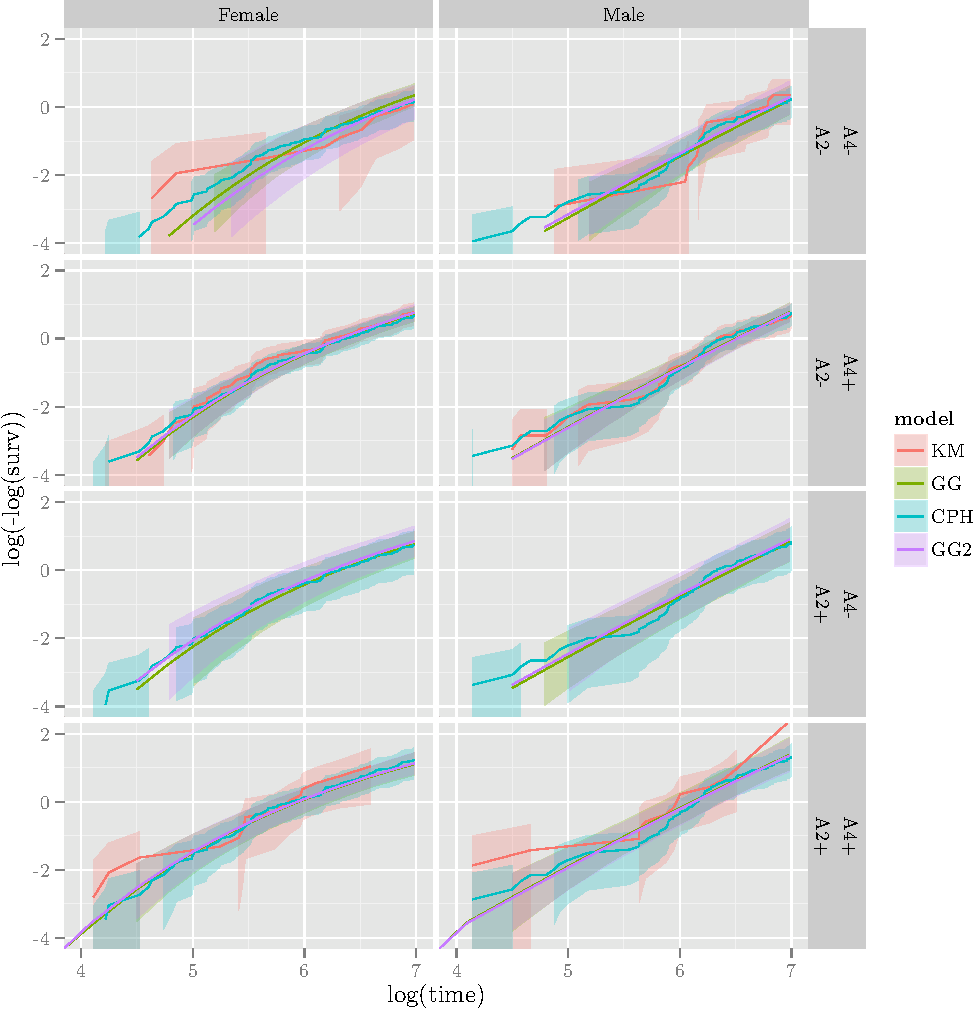
\includegraphics[width=\maxwidth]{figure/05-final-fit-assessment-2-1} 

}


\begin{kframe}\begin{alltt}
\hlkwd{ggplot}\hlstd{(temp.data,} \hlkwd{aes}\hlstd{(}\hlkwc{x} \hlstd{= time,} \hlkwc{y} \hlstd{= surv,} \hlkwc{ymin} \hlstd{= lower,} \hlkwc{ymax} \hlstd{= upper,} \hlkwc{colour} \hlstd{= model,} \hlkwc{fill} \hlstd{= model))} \hlopt{+}
        \hlkwd{geom_ribbon}\hlstd{(}\hlkwc{alpha} \hlstd{=} \hlnum{0.25}\hlstd{,} \hlkwc{colour} \hlstd{=} \hlnum{NA}\hlstd{)} \hlopt{+}
        \hlkwd{geom_line}\hlstd{()} \hlopt{+} \hlkwd{xlim}\hlstd{(}\hlnum{0}\hlstd{,} \hlnum{2000}\hlstd{)} \hlopt{+} \hlkwd{ylim}\hlstd{(}\hlnum{0}\hlstd{,} \hlnum{1}\hlstd{)} \hlopt{+}
        \hlkwd{facet_grid}\hlstd{(A2} \hlopt{~} \hlstd{A4} \hlopt{~} \hlstd{Sex)}
\end{alltt}


{\ttfamily\noindent\color{warningcolor}{\#\# Warning: Removed 4 rows containing missing values (geom\_path).}}

{\ttfamily\noindent\color{warningcolor}{\#\# Warning: Removed 2 rows containing missing values (geom\_path).}}

{\ttfamily\noindent\color{warningcolor}{\#\# Warning: Removed 5 rows containing missing values (geom\_path).}}

{\ttfamily\noindent\color{warningcolor}{\#\# Warning: Removed 1 rows containing missing values (geom\_path).}}

{\ttfamily\noindent\color{warningcolor}{\#\# Warning: Removed 3 rows containing missing values (geom\_path).}}

{\ttfamily\noindent\color{warningcolor}{\#\# Warning: Removed 1 rows containing missing values (geom\_path).}}

{\ttfamily\noindent\color{warningcolor}{\#\# Warning: Removed 3 rows containing missing values (geom\_path).}}

{\ttfamily\noindent\color{warningcolor}{\#\# Warning: Removed 1 rows containing missing values (geom\_path).}}\end{kframe}

{\centering 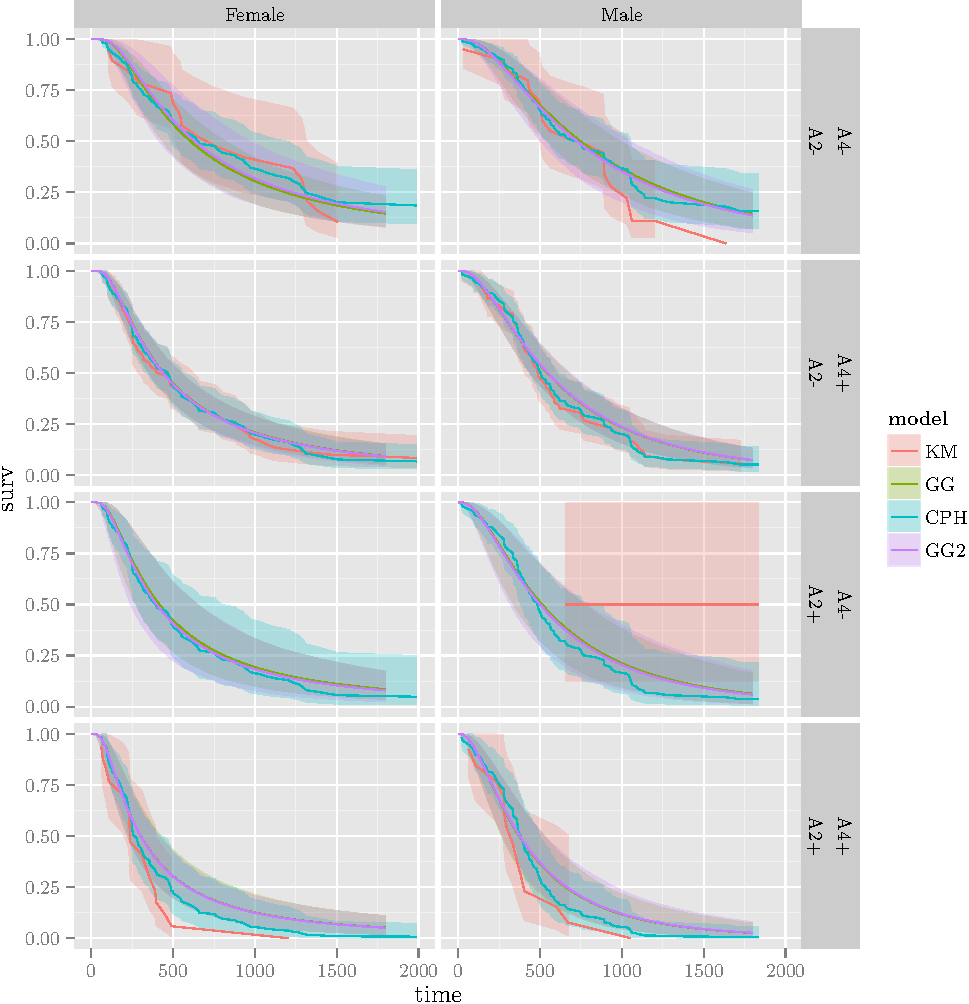
\includegraphics[width=\maxwidth]{figure/05-final-fit-assessment-2-2} 

}



\end{knitrout}

An alternative take, showing errors with the KMs only.
\begin{knitrout}
\definecolor{shadecolor}{rgb}{0.969, 0.969, 0.969}\color{fgcolor}\begin{kframe}
\begin{alltt}
\hlstd{temp.data}\hlopt{$}\hlstd{lower[temp.data}\hlopt{$}\hlstd{model} \hlopt{!=} \hlstr{"KM"}\hlstd{]} \hlkwb{=} \hlnum{NA}
\hlstd{temp.data}\hlopt{$}\hlstd{upper[temp.data}\hlopt{$}\hlstd{model} \hlopt{!=} \hlstr{"KM"}\hlstd{]} \hlkwb{=} \hlnum{NA}
\hlkwd{ggplot}\hlstd{(temp.data,} \hlkwd{aes}\hlstd{(}\hlkwc{x} \hlstd{=} \hlkwd{log}\hlstd{(time),} \hlkwc{y} \hlstd{=} \hlkwd{log}\hlstd{(}\hlopt{-}\hlkwd{log}\hlstd{(surv)),} \hlkwc{ymin} \hlstd{=} \hlkwd{log}\hlstd{(}\hlopt{-}\hlkwd{log}\hlstd{(lower)),} \hlkwc{ymax} \hlstd{=} \hlkwd{log}\hlstd{(}\hlopt{-}\hlkwd{log}\hlstd{(upper)),} \hlkwc{colour} \hlstd{= model,} \hlkwc{fill} \hlstd{= model))} \hlopt{+}
        \hlkwd{geom_ribbon}\hlstd{(}\hlkwc{alpha} \hlstd{=} \hlnum{0.25}\hlstd{,} \hlkwc{colour} \hlstd{=} \hlnum{NA}\hlstd{)} \hlopt{+}
        \hlkwd{geom_line}\hlstd{()} \hlopt{+}
        \hlkwd{xlim}\hlstd{(}\hlnum{4}\hlstd{,} \hlnum{7}\hlstd{)} \hlopt{+} \hlkwd{ylim}\hlstd{(}\hlopt{-}\hlnum{4}\hlstd{,} \hlnum{2}\hlstd{)} \hlopt{+}
        \hlkwd{facet_grid}\hlstd{(A2} \hlopt{~} \hlstd{A4} \hlopt{~} \hlstd{Sex)}
\end{alltt}


{\ttfamily\noindent\color{warningcolor}{\#\# Warning: Removed 75 rows containing missing values (geom\_path).}}

{\ttfamily\noindent\color{warningcolor}{\#\# Warning: Removed 70 rows containing missing values (geom\_path).}}

{\ttfamily\noindent\color{warningcolor}{\#\# Warning: Removed 76 rows containing missing values (geom\_path).}}

{\ttfamily\noindent\color{warningcolor}{\#\# Warning: Removed 68 rows containing missing values (geom\_path).}}

{\ttfamily\noindent\color{warningcolor}{\#\# Warning: Removed 66 rows containing missing values (geom\_path).}}

{\ttfamily\noindent\color{warningcolor}{\#\# Warning: Removed 63 rows containing missing values (geom\_path).}}

{\ttfamily\noindent\color{warningcolor}{\#\# Warning: Removed 66 rows containing missing values (geom\_path).}}

{\ttfamily\noindent\color{warningcolor}{\#\# Warning: Removed 64 rows containing missing values (geom\_path).}}\end{kframe}

{\centering 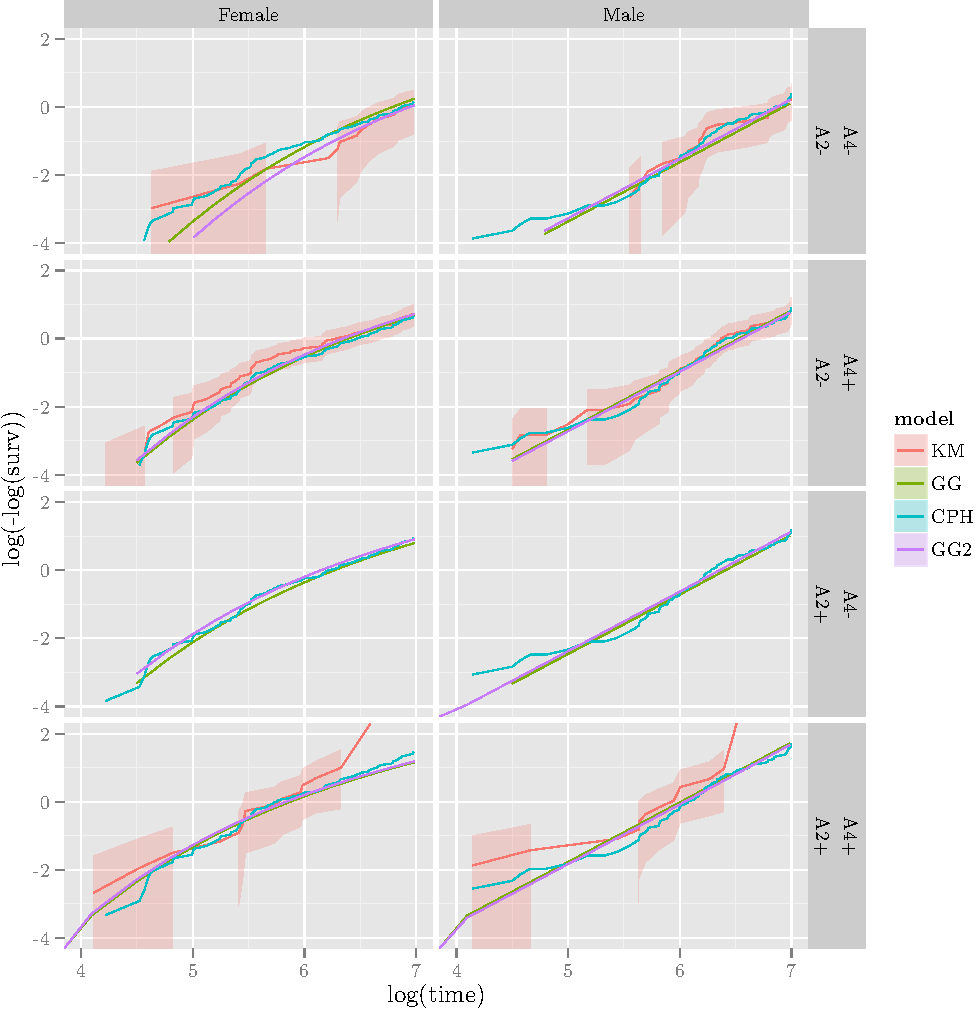
\includegraphics[width=\maxwidth]{figure/05-final-fit-assessment-3-1} 

}


\begin{kframe}\begin{alltt}
\hlkwd{ggplot}\hlstd{(temp.data,} \hlkwd{aes}\hlstd{(}\hlkwc{x} \hlstd{= time,} \hlkwc{y} \hlstd{= surv,} \hlkwc{ymin} \hlstd{= lower,} \hlkwc{ymax} \hlstd{= upper,} \hlkwc{colour} \hlstd{= model,} \hlkwc{fill} \hlstd{= model))} \hlopt{+}
        \hlkwd{geom_ribbon}\hlstd{(}\hlkwc{alpha} \hlstd{=} \hlnum{0.25}\hlstd{,} \hlkwc{colour} \hlstd{=} \hlnum{NA}\hlstd{)} \hlopt{+}
        \hlkwd{geom_line}\hlstd{()} \hlopt{+} \hlkwd{xlim}\hlstd{(}\hlnum{0}\hlstd{,} \hlnum{2000}\hlstd{)} \hlopt{+} \hlkwd{ylim}\hlstd{(}\hlnum{0}\hlstd{,} \hlnum{1}\hlstd{)} \hlopt{+}
        \hlkwd{facet_grid}\hlstd{(A2} \hlopt{~} \hlstd{A4} \hlopt{~} \hlstd{Sex)}
\end{alltt}


{\ttfamily\noindent\color{warningcolor}{\#\# Warning: Removed 4 rows containing missing values (geom\_path).}}

{\ttfamily\noindent\color{warningcolor}{\#\# Warning: Removed 2 rows containing missing values (geom\_path).}}

{\ttfamily\noindent\color{warningcolor}{\#\# Warning: Removed 5 rows containing missing values (geom\_path).}}

{\ttfamily\noindent\color{warningcolor}{\#\# Warning: Removed 1 rows containing missing values (geom\_path).}}

{\ttfamily\noindent\color{warningcolor}{\#\# Warning: Removed 3 rows containing missing values (geom\_path).}}

{\ttfamily\noindent\color{warningcolor}{\#\# Warning: Removed 1 rows containing missing values (geom\_path).}}

{\ttfamily\noindent\color{warningcolor}{\#\# Warning: Removed 3 rows containing missing values (geom\_path).}}

{\ttfamily\noindent\color{warningcolor}{\#\# Warning: Removed 1 rows containing missing values (geom\_path).}}\end{kframe}

{\centering 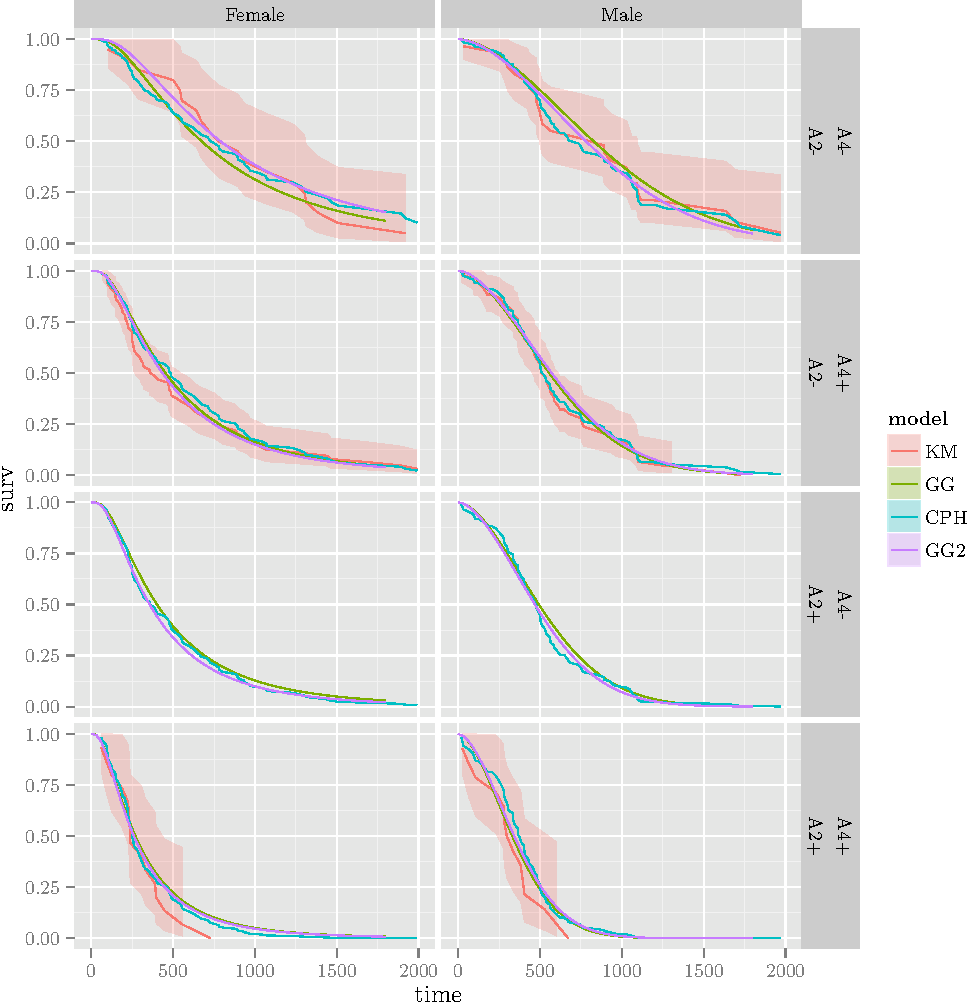
\includegraphics[width=\maxwidth]{figure/05-final-fit-assessment-3-2} 

}



\end{knitrout}

\begin{knitrout}
\definecolor{shadecolor}{rgb}{0.969, 0.969, 0.969}\color{fgcolor}\begin{kframe}
\begin{alltt}
\hlstd{temp.data}\hlopt{$}\hlstd{lower[temp.data}\hlopt{$}\hlstd{model} \hlopt{!=} \hlstr{"KM"}\hlstd{]} \hlkwb{=} \hlnum{NA}
\hlstd{temp.data}\hlopt{$}\hlstd{upper[temp.data}\hlopt{$}\hlstd{model} \hlopt{!=} \hlstr{"KM"}\hlstd{]} \hlkwb{=} \hlnum{NA}
\hlstd{temp.data} \hlkwb{=} \hlstd{temp.data[temp.data}\hlopt{$}\hlstd{model} \hlopt{!=} \hlstr{"GG2"}\hlstd{,]}
\hlstd{temp.data}\hlopt{$}\hlstd{model} \hlkwb{=} \hlkwd{c}\hlstd{(}\hlstr{"KM"} \hlstd{=} \hlstr{"Kaplan-Meier"}\hlstd{,} \hlstr{"GG"} \hlstd{=} \hlstr{"GG1"}\hlstd{,} \hlstr{"CPH"} \hlstd{=} \hlstr{"CP1"}\hlstd{)[temp.data}\hlopt{$}\hlstd{model]}
\hlkwd{ggplot}\hlstd{(temp.data,} \hlkwd{aes}\hlstd{(}\hlkwc{x} \hlstd{=} \hlkwd{log}\hlstd{(time),} \hlkwc{y} \hlstd{=} \hlkwd{log}\hlstd{(}\hlopt{-}\hlkwd{log}\hlstd{(surv)),} \hlkwc{ymin} \hlstd{=} \hlkwd{log}\hlstd{(}\hlopt{-}\hlkwd{log}\hlstd{(lower)),} \hlkwc{ymax} \hlstd{=} \hlkwd{log}\hlstd{(}\hlopt{-}\hlkwd{log}\hlstd{(upper)),} \hlkwc{colour} \hlstd{= model,} \hlkwc{fill} \hlstd{= model))} \hlopt{+}
        \hlkwd{geom_ribbon}\hlstd{(}\hlkwc{alpha} \hlstd{=} \hlnum{0.25}\hlstd{,} \hlkwc{colour} \hlstd{=} \hlnum{NA}\hlstd{)} \hlopt{+}
        \hlkwd{geom_line}\hlstd{()} \hlopt{+}
        \hlkwd{xlim}\hlstd{(}\hlnum{4}\hlstd{,} \hlnum{7}\hlstd{)} \hlopt{+} \hlkwd{ylim}\hlstd{(}\hlopt{-}\hlnum{4}\hlstd{,} \hlnum{2}\hlstd{)} \hlopt{+}
        \hlkwd{facet_grid}\hlstd{(A2} \hlopt{~} \hlstd{A4} \hlopt{~} \hlstd{Sex)}
\end{alltt}


{\ttfamily\noindent\color{warningcolor}{\#\# Warning: Removed 50 rows containing missing values (geom\_path).}}

{\ttfamily\noindent\color{warningcolor}{\#\# Warning: Removed 45 rows containing missing values (geom\_path).}}

{\ttfamily\noindent\color{warningcolor}{\#\# Warning: Removed 51 rows containing missing values (geom\_path).}}

{\ttfamily\noindent\color{warningcolor}{\#\# Warning: Removed 43 rows containing missing values (geom\_path).}}

{\ttfamily\noindent\color{warningcolor}{\#\# Warning: Removed 41 rows containing missing values (geom\_path).}}

{\ttfamily\noindent\color{warningcolor}{\#\# Warning: Removed 38 rows containing missing values (geom\_path).}}

{\ttfamily\noindent\color{warningcolor}{\#\# Warning: Removed 41 rows containing missing values (geom\_path).}}

{\ttfamily\noindent\color{warningcolor}{\#\# Warning: Removed 39 rows containing missing values (geom\_path).}}\end{kframe}

{\centering 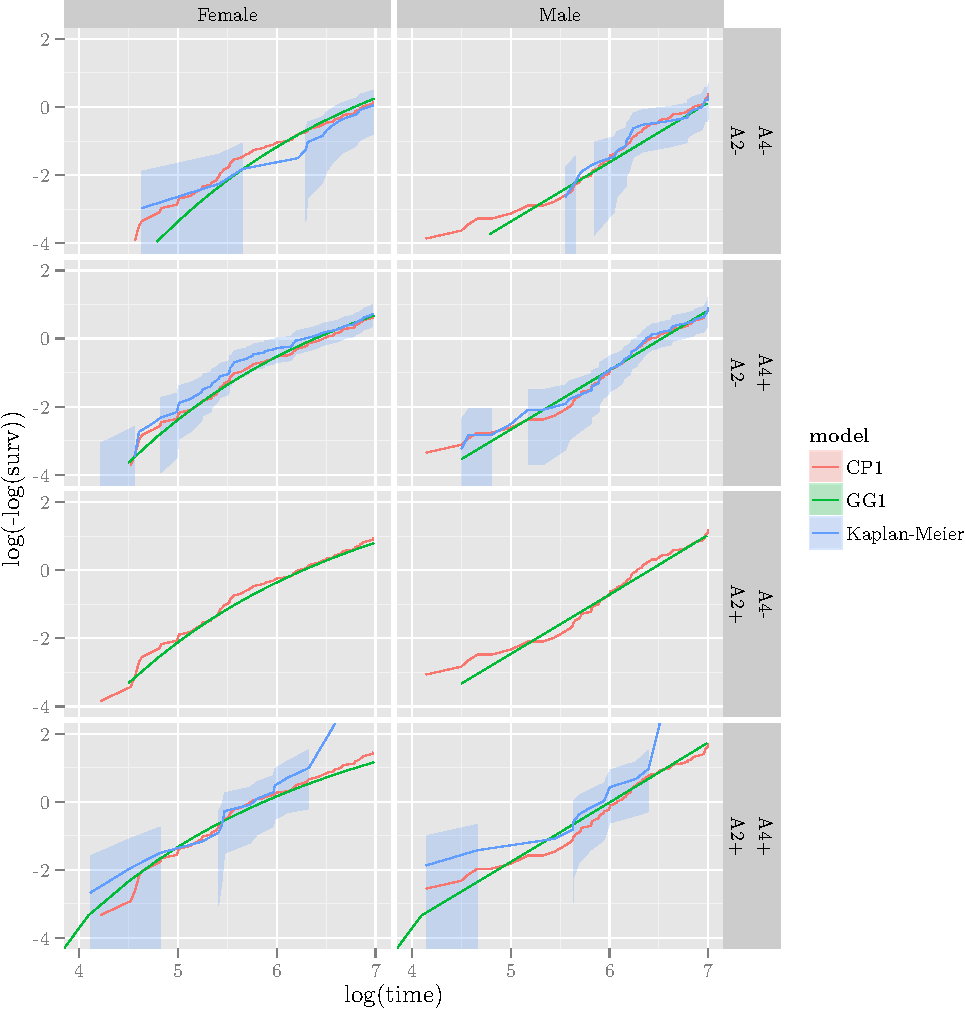
\includegraphics[width=\maxwidth]{figure/05-final-fit-assessment-4-1} 

}


\begin{kframe}\begin{alltt}
\hlkwd{ggplot}\hlstd{(temp.data,} \hlkwd{aes}\hlstd{(}\hlkwc{x} \hlstd{= time,} \hlkwc{y} \hlstd{= surv,} \hlkwc{ymin} \hlstd{= lower,} \hlkwc{ymax} \hlstd{= upper,} \hlkwc{colour} \hlstd{= model,} \hlkwc{fill} \hlstd{= model))} \hlopt{+}
        \hlkwd{geom_ribbon}\hlstd{(}\hlkwc{alpha} \hlstd{=} \hlnum{0.25}\hlstd{,} \hlkwc{colour} \hlstd{=} \hlnum{NA}\hlstd{)} \hlopt{+}
        \hlkwd{geom_line}\hlstd{()} \hlopt{+} \hlkwd{xlim}\hlstd{(}\hlnum{0}\hlstd{,} \hlnum{2000}\hlstd{)} \hlopt{+} \hlkwd{ylim}\hlstd{(}\hlnum{0}\hlstd{,} \hlnum{1}\hlstd{)} \hlopt{+}
        \hlkwd{facet_grid}\hlstd{(A2} \hlopt{~} \hlstd{A4} \hlopt{~} \hlstd{Sex)}
\end{alltt}


{\ttfamily\noindent\color{warningcolor}{\#\# Warning: Removed 4 rows containing missing values (geom\_path).}}

{\ttfamily\noindent\color{warningcolor}{\#\# Warning: Removed 2 rows containing missing values (geom\_path).}}

{\ttfamily\noindent\color{warningcolor}{\#\# Warning: Removed 5 rows containing missing values (geom\_path).}}

{\ttfamily\noindent\color{warningcolor}{\#\# Warning: Removed 1 rows containing missing values (geom\_path).}}

{\ttfamily\noindent\color{warningcolor}{\#\# Warning: Removed 3 rows containing missing values (geom\_path).}}

{\ttfamily\noindent\color{warningcolor}{\#\# Warning: Removed 1 rows containing missing values (geom\_path).}}

{\ttfamily\noindent\color{warningcolor}{\#\# Warning: Removed 3 rows containing missing values (geom\_path).}}

{\ttfamily\noindent\color{warningcolor}{\#\# Warning: Removed 1 rows containing missing values (geom\_path).}}\end{kframe}

{\centering 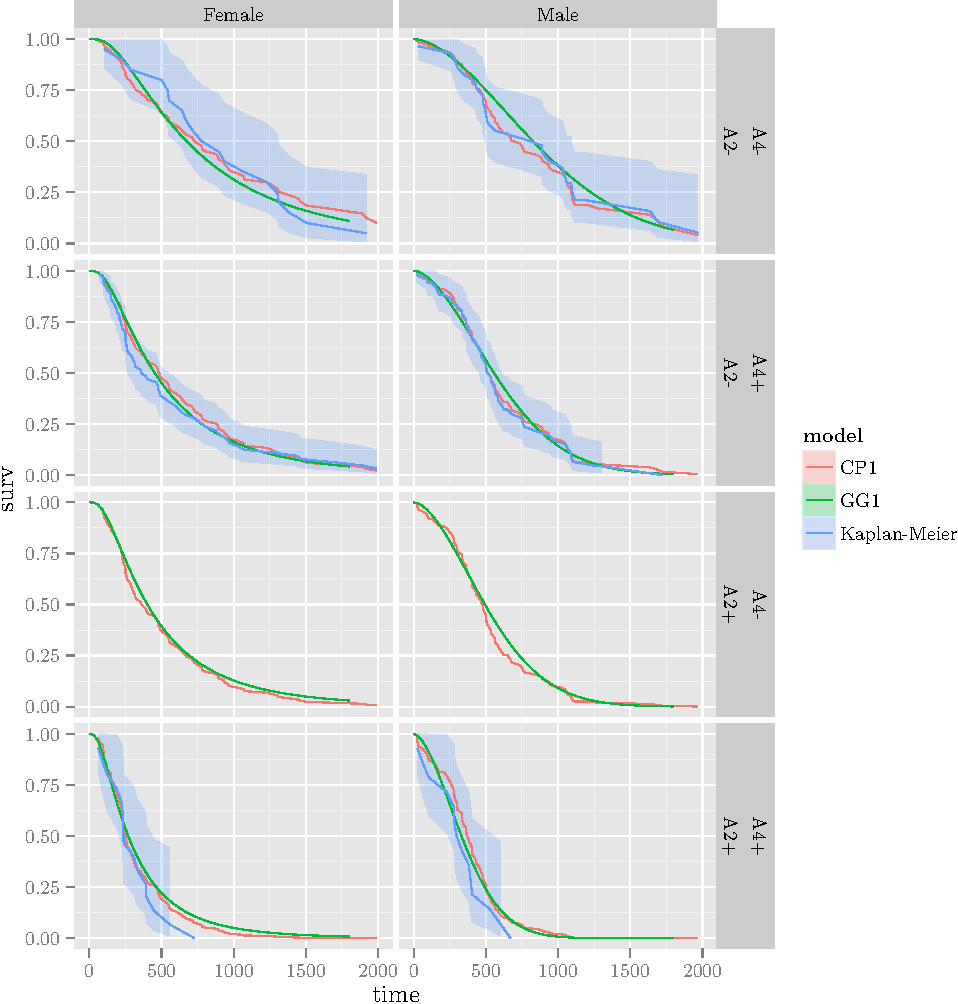
\includegraphics[width=\maxwidth]{figure/05-final-fit-assessment-4-2} 

}



\end{knitrout}


\section{Model selection}
It looks like that's as far as we can go with tweaking the fits.  Time to put the different models against each other on the holdout data, and choose a winner.

DIY IBS, wooo.
\begin{knitrout}
\definecolor{shadecolor}{rgb}{0.969, 0.969, 0.969}\color{fgcolor}\begin{kframe}
\begin{alltt}
\hlstd{calcIBS} \hlkwb{=} \hlkwa{function}\hlstd{(}\hlkwc{surv}\hlstd{,} \hlkwc{pred}\hlstd{,} \hlkwc{pred_times}\hlstd{,} \hlkwc{max_time}\hlstd{)}
\hlstd{\{}
        \hlkwd{stopifnot}\hlstd{(}\hlkwd{nrow}\hlstd{(surv)} \hlopt{==} \hlkwd{nrow}\hlstd{(pred)} \hlopt{&&} \hlkwd{length}\hlstd{(pred_times)} \hlopt{==} \hlkwd{ncol}\hlstd{(pred))}

        \hlstd{n} \hlkwb{=} \hlkwd{nrow}\hlstd{(surv)}
        \hlstd{marg_survfit} \hlkwb{=} \hlkwd{survfit}\hlstd{(surv} \hlopt{~} \hlnum{1}\hlstd{)}
        \hlstd{marg_censfit} \hlkwb{=} \hlkwd{survfit}\hlstd{(}\hlkwd{Surv}\hlstd{(surv[,}\hlnum{1}\hlstd{],} \hlopt{!}\hlstd{surv[,}\hlnum{2}\hlstd{])} \hlopt{~} \hlnum{1}\hlstd{)}
        \hlstd{marg_surv_func} \hlkwb{=} \hlkwd{approxfun}\hlstd{(marg_survfit}\hlopt{$}\hlstd{time, marg_survfit}\hlopt{$}\hlstd{surv,} \hlkwc{method} \hlstd{=} \hlstr{"constant"}\hlstd{,} \hlkwc{yleft} \hlstd{=} \hlnum{1}\hlstd{,} \hlkwc{yright} \hlstd{=} \hlnum{0}\hlstd{,} \hlkwc{rule} \hlstd{=} \hlnum{2}\hlopt{:}\hlnum{1}\hlstd{,} \hlkwc{f} \hlstd{=} \hlnum{0}\hlstd{)}
        \hlstd{marg_cens_func} \hlkwb{=} \hlkwd{approxfun}\hlstd{(marg_censfit}\hlopt{$}\hlstd{time, marg_censfit}\hlopt{$}\hlstd{surv,} \hlkwc{method} \hlstd{=} \hlstr{"constant"}\hlstd{,} \hlkwc{yleft} \hlstd{=} \hlnum{1}\hlstd{,} \hlkwc{yright} \hlstd{=} \hlnum{0}\hlstd{,} \hlkwc{rule} \hlstd{=} \hlnum{2}\hlopt{:}\hlnum{1}\hlstd{,} \hlkwc{f} \hlstd{=} \hlnum{0}\hlstd{)}

        \hlstd{pred_funcs} \hlkwb{=} \hlkwd{apply}\hlstd{(pred,} \hlnum{1}\hlstd{,} \hlkwa{function}\hlstd{(}\hlkwc{pat_preds}\hlstd{)} \hlkwd{approxfun}\hlstd{(pred_times, pat_preds,} \hlkwc{yleft} \hlstd{=} \hlnum{1}\hlstd{,} \hlkwc{yright} \hlstd{=} \hlkwd{min}\hlstd{(pat_preds),} \hlkwc{rule} \hlstd{=} \hlnum{2}\hlstd{))}

        \hlstd{indiv_patient_bsc} \hlkwb{=} \hlkwa{function}\hlstd{(}\hlkwc{pat_i}\hlstd{,} \hlkwc{tstars}\hlstd{)}
        \hlstd{\{}
                \hlstd{observed_time} \hlkwb{=} \hlstd{surv[pat_i,} \hlnum{1}\hlstd{]}
                \hlstd{observed_event} \hlkwb{=} \hlstd{surv[pat_i,} \hlnum{2}\hlstd{]}
                \hlstd{pred_func} \hlkwb{=} \hlstd{pred_funcs[[pat_i]]}
                \hlstd{category} \hlkwb{=} \hlnum{1}\hlopt{*}\hlstd{(observed_time} \hlopt{<=} \hlstd{tstars} \hlopt{&} \hlstd{observed_event)} \hlopt{+} \hlnum{2}\hlopt{*}\hlstd{(observed_time} \hlopt{>} \hlstd{tstars)} \hlopt{+} \hlnum{3}\hlopt{*}\hlstd{(observed_time} \hlopt{<=} \hlstd{tstars} \hlopt{& !}\hlstd{observed_event)}
                \hlstd{bsc} \hlkwb{=} \hlkwd{rep}\hlstd{(}\hlnum{NA}\hlstd{,} \hlkwd{length}\hlstd{(tstars))}
                \hlstd{bsc[category} \hlopt{==} \hlnum{1}\hlstd{]} \hlkwb{=} \hlkwd{pred_func}\hlstd{(tstars[category} \hlopt{==} \hlnum{1}\hlstd{])}\hlopt{^}\hlnum{2} \hlopt{/} \hlkwd{marg_cens_func}\hlstd{(observed_time)}
                \hlstd{bsc[category} \hlopt{==} \hlnum{2}\hlstd{]} \hlkwb{=} \hlstd{(}\hlnum{1} \hlopt{-} \hlkwd{pred_func}\hlstd{(tstars[category} \hlopt{==} \hlnum{2}\hlstd{]))}\hlopt{^}\hlnum{2} \hlopt{/} \hlkwd{marg_cens_func}\hlstd{(tstars[category} \hlopt{==} \hlnum{2}\hlstd{])}
                \hlstd{bsc[category} \hlopt{==} \hlnum{3}\hlstd{]} \hlkwb{=} \hlnum{0}
                \hlstd{bsc}
        \hlstd{\}}

        \hlstd{bsc_func} \hlkwb{=} \hlkwa{function}\hlstd{(}\hlkwc{tstars}\hlstd{) \{} \hlkwd{rowMeans}\hlstd{(}\hlkwd{sapply}\hlstd{(}\hlnum{1}\hlopt{:}\hlstd{n,} \hlkwa{function}\hlstd{(}\hlkwc{pat_i}\hlstd{)} \hlkwd{indiv_patient_bsc}\hlstd{(pat_i, tstars))) \}}

        \hlstd{weight_func} \hlkwb{=} \hlkwa{function}\hlstd{(}\hlkwc{tstars}\hlstd{) \{ (}\hlnum{1} \hlopt{-} \hlkwd{marg_surv_func}\hlstd{(tstars))} \hlopt{/} \hlstd{(}\hlnum{1} \hlopt{-} \hlkwd{marg_surv_func}\hlstd{(max_time)) \}}

        \hlcom{# Be slack and do trapezoidal int. with a fine grid.  It should be possible }
        \hlcom{# to calulate the int. exactly but I cbfed.}
        \hlstd{int_grid} \hlkwb{=} \hlkwd{seq}\hlstd{(}\hlnum{0}\hlstd{, max_time,} \hlkwc{length.out} \hlstd{=} \hlnum{1e3}\hlstd{)}
        \hlstd{bsc_vals} \hlkwb{=} \hlkwd{bsc_func}\hlstd{(int_grid)}
        \hlstd{weight_vals} \hlkwb{=} \hlkwd{weight_func}\hlstd{(int_grid)}
        \hlstd{int_vals} \hlkwb{=} \hlstd{bsc_vals} \hlopt{*} \hlstd{weight_vals}
        \hlstd{ibsc} \hlkwb{=} \hlstd{(}\hlnum{2}\hlopt{*}\hlkwd{sum}\hlstd{(int_vals)} \hlopt{-} \hlstd{int_vals[}\hlnum{1}\hlstd{]} \hlopt{-} \hlstd{int_vals[}\hlkwd{length}\hlstd{(int_vals)])} \hlopt{*} \hlstd{(}\hlkwd{diff}\hlstd{(}\hlkwd{range}\hlstd{(int_grid)))} \hlopt{/} \hlstd{(}\hlnum{2}\hlopt{*}\hlkwd{length}\hlstd{(int_vals))}

        \hlkwd{return}\hlstd{(}\hlkwd{list}\hlstd{(}\hlkwc{bsc} \hlstd{= bsc_vals,} \hlkwc{weights} \hlstd{= weight_vals,} \hlkwc{eval_times} \hlstd{= int_grid,} \hlkwc{ibsc} \hlstd{= ibsc))}
\hlstd{\}}
\end{alltt}
\end{kframe}
\end{knitrout}

Calculate survival probability predictions for each of the models, on the validation data.
\begin{knitrout}
\definecolor{shadecolor}{rgb}{0.969, 0.969, 0.969}\color{fgcolor}\begin{kframe}
\begin{alltt}
\hlstd{ibs_times} \hlkwb{=} \hlkwd{sort}\hlstd{(}\hlkwd{unique}\hlstd{(data.val}\hlopt{$}\hlstd{Time))}
\hlstd{ibs_preds_gg} \hlkwb{=} \hlkwd{as.matrix}\hlstd{(}\hlkwd{t}\hlstd{(}\hlkwd{sapply}\hlstd{(}\hlkwd{summary}\hlstd{(fit.gg,} \hlkwc{newdata} \hlstd{= data.val,} \hlkwc{type} \hlstd{=} \hlstr{"survival"}\hlstd{,} \hlkwc{t} \hlstd{= ibs_times),} \hlkwa{function}\hlstd{(}\hlkwc{x}\hlstd{) x}\hlopt{$}\hlstd{est)))}
\hlstd{ibs_preds_gg2} \hlkwb{=} \hlkwd{as.matrix}\hlstd{(}\hlkwd{t}\hlstd{(}\hlkwd{sapply}\hlstd{(}\hlkwd{summary}\hlstd{(fit.gg2,} \hlkwc{newdata} \hlstd{= data.val,} \hlkwc{type} \hlstd{=} \hlstr{"survival"}\hlstd{,} \hlkwc{t} \hlstd{= ibs_times),} \hlkwa{function}\hlstd{(}\hlkwc{x}\hlstd{) x}\hlopt{$}\hlstd{est)))}
\hlstd{temp_cox_preds} \hlkwb{=} \hlkwd{survfit}\hlstd{(fit.cph,} \hlkwc{newdata} \hlstd{= data.val)}
\hlstd{ibs_preds_cph} \hlkwb{=} \hlkwd{simplify2array}\hlstd{(}\hlkwd{tapply}\hlstd{(}\hlnum{1}\hlopt{:}\hlkwd{length}\hlstd{(temp_cox_preds}\hlopt{$}\hlstd{time),} \hlkwd{rep}\hlstd{(}\hlkwd{names}\hlstd{(temp_cox_preds}\hlopt{$}\hlstd{strata), temp_cox_preds}\hlopt{$}\hlstd{strata),} \hlkwa{function}\hlstd{(}\hlkwc{strat_i}\hlstd{) \{}
        \hlkwd{approx}\hlstd{(}\hlkwc{x} \hlstd{= temp_cox_preds}\hlopt{$}\hlstd{time[strat_i],} \hlkwc{y} \hlstd{= temp_cox_preds}\hlopt{$}\hlstd{surv[strat_i],} \hlkwc{xout} \hlstd{= ibs_times,} \hlkwc{method} \hlstd{=} \hlstr{"constant"}\hlstd{,} \hlkwc{yleft} \hlstd{=} \hlnum{1}\hlstd{,} \hlkwc{rule} \hlstd{=} \hlnum{2}\hlstd{,} \hlkwc{f} \hlstd{=} \hlnum{0}\hlstd{)}\hlopt{$}\hlstd{y \} ))}
\hlstd{ibs_preds_cph} \hlkwb{=} \hlkwd{t}\hlstd{(ibs_preds_cph[,}\hlkwd{rownames}\hlstd{(data.val)])}
\hlstd{temp_rsf_preds} \hlkwb{=} \hlkwd{predict}\hlstd{(fit.rsf,} \hlkwc{newdata} \hlstd{= data.val)}
\hlstd{ibs_preds_rsf} \hlkwb{=} \hlkwd{t}\hlstd{(}\hlkwd{apply}\hlstd{(temp_rsf_preds}\hlopt{$}\hlstd{survival,} \hlnum{1}\hlstd{,} \hlkwa{function}\hlstd{(}\hlkwc{survs}\hlstd{)} \hlkwd{approx}\hlstd{(temp_rsf_preds}\hlopt{$}\hlstd{time.interest, survs,} \hlkwc{xout} \hlstd{= ibs_times,} \hlkwc{method} \hlstd{=} \hlstr{"constant"}\hlstd{,} \hlkwc{yleft} \hlstd{=} \hlnum{1}\hlstd{,} \hlkwc{rule} \hlstd{=} \hlnum{2}\hlstd{,} \hlkwc{f} \hlstd{=} \hlnum{0}\hlstd{)}\hlopt{$}\hlstd{y))}
\hlcom{# Patients (from data.val) are in rows, times (from ibs_times) in columns.}

\hlcom{# Add a no-information KM predictor}
\hlstd{temp_km0} \hlkwb{=} \hlkwd{survfit}\hlstd{(}\hlkwd{Surv}\hlstd{(Time, DSD)} \hlopt{~} \hlnum{1}\hlstd{, data)}
\hlstd{ibs_preds_km0} \hlkwb{=} \hlkwd{t}\hlstd{(}\hlkwd{matrix}\hlstd{(}\hlkwd{rep}\hlstd{(}\hlkwd{approx}\hlstd{(temp_km0}\hlopt{$}\hlstd{time, temp_km0}\hlopt{$}\hlstd{surv,} \hlkwc{xout} \hlstd{= ibs_times,} \hlkwc{method} \hlstd{=} \hlstr{"constant"}\hlstd{,} \hlkwc{yleft} \hlstd{=} \hlnum{1}\hlstd{,} \hlkwc{rule} \hlstd{=} \hlnum{2}\hlstd{,} \hlkwc{f} \hlstd{=} \hlnum{0}\hlstd{)}\hlopt{$}\hlstd{y,} \hlkwc{times} \hlstd{=} \hlkwd{nrow}\hlstd{(data.val)),} \hlkwc{ncol} \hlstd{=} \hlkwd{nrow}\hlstd{(data.val)))}
\hlstd{ibs_preds_all} \hlkwb{=} \hlkwd{list}\hlstd{(}\hlkwc{gg} \hlstd{= ibs_preds_gg,} \hlkwc{gg2} \hlstd{= ibs_preds_gg2,} \hlkwc{cph} \hlstd{= ibs_preds_cph,} \hlkwc{rsf} \hlstd{= ibs_preds_rsf,} \hlkwc{km0} \hlstd{= ibs_preds_km0)}
\end{alltt}
\end{kframe}
\end{knitrout}


\begin{knitrout}
\definecolor{shadecolor}{rgb}{0.969, 0.969, 0.969}\color{fgcolor}\begin{kframe}
\begin{alltt}
\hlstd{val.prob.times} \hlkwb{=} \hlkwd{seq}\hlstd{(}\hlnum{0}\hlstd{,} \hlkwd{max}\hlstd{(data.val}\hlopt{$}\hlstd{Time),} \hlnum{1}\hlstd{)}

\hlstd{temp.coefs} \hlkwb{=} \hlkwd{coef}\hlstd{(fit.gg)}
\hlstd{val.linpred.gg} \hlkwb{=} \hlkwd{sapply}\hlstd{(}\hlnum{1}\hlopt{:}\hlkwd{length}\hlstd{(temp.coefs),} \hlkwa{function}\hlstd{(}\hlkwc{coef_i}\hlstd{) \{}
    \hlkwa{if} \hlstd{(}\hlkwd{names}\hlstd{(temp.coefs)[coef_i]} \hlopt \hlkwd{colnames}\hlstd{(data.val)) \{}
        \hlstd{temp.coefs[coef_i]} \hlopt{*} \hlstd{data.val[,}\hlkwd{names}\hlstd{(temp.coefs)[coef_i]]}
    \hlstd{\}} \hlkwa{else if} \hlstd{(}\hlkwd{gsub}\hlstd{(}\hlstr{"TRUE$"}\hlstd{,} \hlstr{""}\hlstd{,} \hlkwd{names}\hlstd{(temp.coefs)[coef_i])} \hlopt \hlkwd{colnames}\hlstd{(data.val)) \{}
        \hlstd{temp.coefs[coef_i]} \hlopt{*} \hlstd{data.val[,}\hlkwd{gsub}\hlstd{(}\hlstr{"TRUE$"}\hlstd{,} \hlstr{""}\hlstd{,} \hlkwd{names}\hlstd{(temp.coefs)[coef_i])]}
    \hlstd{\}} \hlkwa{else} \hlstd{\{}
        \hlkwd{rep}\hlstd{(}\hlnum{0}\hlstd{,} \hlkwd{nrow}\hlstd{(data.val))}
    \hlstd{\} \})}
\hlstd{val.linpred.gg} \hlkwb{=} \hlopt{-}\hlkwd{rowSums}\hlstd{(val.linpred.gg)}   \hlcom{# Negate to bring into concordance with the direction of Cox coefficients (ie higher is now worse)}
\hlstd{temp} \hlkwb{=} \hlkwd{summary}\hlstd{(fit.gg,} \hlkwc{newdata} \hlstd{= data.val,} \hlkwc{ci} \hlstd{=} \hlnum{FALSE}\hlstd{)}
\hlstd{val.prob.gg} \hlkwb{=} \hlkwd{sapply}\hlstd{(temp,} \hlkwa{function}\hlstd{(}\hlkwc{x}\hlstd{)} \hlkwd{approx}\hlstd{(x[,}\hlnum{1}\hlstd{], x[,}\hlnum{2}\hlstd{],} \hlkwc{xout} \hlstd{= val.prob.times,} \hlkwc{yleft} \hlstd{=} \hlnum{1}\hlstd{,} \hlkwc{yright} \hlstd{=} \hlnum{0}\hlstd{,} \hlkwc{rule} \hlstd{=} \hlnum{2}\hlstd{)}\hlopt{$}\hlstd{y)}
\hlkwd{colnames}\hlstd{(val.prob.gg)} \hlkwb{=} \hlkwd{rownames}\hlstd{(data.val)}

\hlstd{temp.coefs} \hlkwb{=} \hlkwd{coef}\hlstd{(fit.gg2)}
\hlstd{val.linpred.gg2} \hlkwb{=} \hlkwd{sapply}\hlstd{(}\hlnum{1}\hlopt{:}\hlkwd{length}\hlstd{(temp.coefs),} \hlkwa{function}\hlstd{(}\hlkwc{coef_i}\hlstd{) \{}
    \hlkwa{if} \hlstd{(}\hlkwd{names}\hlstd{(temp.coefs)[coef_i]} \hlopt \hlkwd{colnames}\hlstd{(data.val)) \{}
        \hlstd{temp.coefs[coef_i]} \hlopt{*} \hlstd{data.val[,}\hlkwd{names}\hlstd{(temp.coefs)[coef_i]]}
    \hlstd{\}} \hlkwa{else if} \hlstd{(}\hlkwd{gsub}\hlstd{(}\hlstr{"TRUE$"}\hlstd{,} \hlstr{""}\hlstd{,} \hlkwd{names}\hlstd{(temp.coefs)[coef_i])} \hlopt \hlkwd{colnames}\hlstd{(data.val)) \{}
        \hlstd{temp.coefs[coef_i]} \hlopt{*} \hlstd{data.val[,}\hlkwd{gsub}\hlstd{(}\hlstr{"TRUE$"}\hlstd{,} \hlstr{""}\hlstd{,} \hlkwd{names}\hlstd{(temp.coefs)[coef_i])]}
    \hlstd{\}} \hlkwa{else} \hlstd{\{}
        \hlkwd{rep}\hlstd{(}\hlnum{0}\hlstd{,} \hlkwd{nrow}\hlstd{(data.val))}
    \hlstd{\} \})}
\hlstd{val.linpred.gg2} \hlkwb{=} \hlopt{-}\hlkwd{rowSums}\hlstd{(val.linpred.gg2)}   \hlcom{# Negate to bring into concordance with the direction of Cox coefficients (ie higher is now worse)}
\hlstd{temp} \hlkwb{=} \hlkwd{summary}\hlstd{(fit.gg2,} \hlkwc{newdata} \hlstd{= data.val,} \hlkwc{ci} \hlstd{=} \hlnum{FALSE}\hlstd{)}
\hlstd{val.prob.gg2} \hlkwb{=} \hlkwd{sapply}\hlstd{(temp,} \hlkwa{function}\hlstd{(}\hlkwc{x}\hlstd{)} \hlkwd{approx}\hlstd{(x[,}\hlnum{1}\hlstd{], x[,}\hlnum{2}\hlstd{],} \hlkwc{xout} \hlstd{= val.prob.times,} \hlkwc{yleft} \hlstd{=} \hlnum{1}\hlstd{,} \hlkwc{yright} \hlstd{=} \hlnum{0}\hlstd{,} \hlkwc{rule} \hlstd{=} \hlnum{2}\hlstd{)}\hlopt{$}\hlstd{y)}
\hlkwd{colnames}\hlstd{(val.prob.gg2)} \hlkwb{=} \hlkwd{rownames}\hlstd{(data.val)}

\hlstd{val.linpred.cph} \hlkwb{=} \hlkwd{predict}\hlstd{(fit.cph,} \hlkwc{newdata} \hlstd{= data.val)}
\hlstd{temp} \hlkwb{=} \hlkwd{survfit}\hlstd{(fit.cph,} \hlkwc{newdata} \hlstd{= data.val)}
\hlstd{val.prob.cph} \hlkwb{=} \hlkwd{simplify2array}\hlstd{(}\hlkwd{tapply}\hlstd{(}\hlnum{1}\hlopt{:}\hlkwd{length}\hlstd{(temp}\hlopt{$}\hlstd{surv),} \hlkwd{rep}\hlstd{(}\hlkwd{names}\hlstd{(temp}\hlopt{$}\hlstd{strata), temp}\hlopt{$}\hlstd{strata),} \hlkwa{function}\hlstd{(}\hlkwc{is}\hlstd{)} \hlkwd{approx}\hlstd{(temp}\hlopt{$}\hlstd{time[is], temp}\hlopt{$}\hlstd{surv[is], val.prob.times,} \hlkwc{yleft} \hlstd{=} \hlnum{1}\hlstd{,} \hlkwc{yright} \hlstd{=} \hlnum{0}\hlstd{,} \hlkwc{rule} \hlstd{=} \hlnum{2}\hlstd{)}\hlopt{$}\hlstd{y))[,}\hlkwd{rownames}\hlstd{(data.val)]}

\hlstd{temp} \hlkwb{=} \hlkwd{predict}\hlstd{(fit.rsf,} \hlkwc{newdata} \hlstd{= data.val)}
\hlcom{# val.linpred.rsf = temp$predicted}
\hlcom{# Median survival time:}
\hlstd{val.linpred.rsf} \hlkwb{=} \hlkwd{apply}\hlstd{(temp}\hlopt{$}\hlstd{survival,} \hlnum{1}\hlstd{,} \hlkwa{function}\hlstd{(}\hlkwc{s1}\hlstd{) \{}
    \hlstd{sfunc} \hlkwb{=} \hlkwd{approxfun}\hlstd{(temp}\hlopt{$}\hlstd{time.interest, s1,} \hlkwc{yleft} \hlstd{=} \hlnum{1}\hlstd{,} \hlkwc{yright} \hlstd{=} \hlnum{0}\hlstd{,} \hlkwc{rule} \hlstd{=} \hlnum{2}\hlstd{)}
    \hlstd{med} \hlkwb{=} \hlkwd{uniroot}\hlstd{(}\hlkwa{function}\hlstd{(}\hlkwc{x}\hlstd{)} \hlkwd{sfunc}\hlstd{(x)} \hlopt{-} \hlnum{0.5}\hlstd{,} \hlkwc{lower} \hlstd{=} \hlkwd{min}\hlstd{(temp}\hlopt{$}\hlstd{time.interest),} \hlkwc{upper} \hlstd{=} \hlkwd{max}\hlstd{(temp}\hlopt{$}\hlstd{time.interest))}\hlopt{$}\hlstd{root}
    \hlstd{med}
\hlstd{\})}
\hlstd{val.linpred.rsf} \hlkwb{=} \hlopt{-}\hlstd{val.linpred.rsf}
\hlstd{val.prob.rsf} \hlkwb{=} \hlkwd{apply}\hlstd{(temp}\hlopt{$}\hlstd{survival,} \hlnum{1}\hlstd{,} \hlkwa{function}\hlstd{(}\hlkwc{s1}\hlstd{)} \hlkwd{approx}\hlstd{(temp}\hlopt{$}\hlstd{time.interest, s1,} \hlkwc{xout} \hlstd{= val.prob.times,} \hlkwc{yleft} \hlstd{=} \hlnum{1}\hlstd{,} \hlkwc{yright} \hlstd{=} \hlnum{0}\hlstd{,} \hlkwc{rule} \hlstd{=} \hlnum{2}\hlstd{)}\hlopt{$}\hlstd{y)}
\hlkwd{colnames}\hlstd{(val.prob.rsf)} \hlkwb{=} \hlkwd{rownames}\hlstd{(data.val)}

\hlkwd{summary}\hlstd{(}\hlkwd{coxph}\hlstd{(}\hlkwd{Surv}\hlstd{(Time, DSD)} \hlopt{~} \hlstd{val.linpred.gg, data.val))}
\end{alltt}
\begin{verbatim}
## Call:
## coxph(formula = Surv(Time, DSD) ~ val.linpred.gg, data = data.val)
## 
##   n= 48, number of events= 46 
## 
##                 coef exp(coef) se(coef)   z Pr(>|z|)
## val.linpred.gg 0.160     1.173    0.397 0.4     0.69
## 
##                exp(coef) exp(-coef) lower .95 upper .95
## val.linpred.gg      1.17      0.852     0.539      2.56
## 
## Concordance= 0.554  (se = 0.05 )
## Rsquare= 0.003   (max possible= 0.997 )
## Likelihood ratio test= 0.16  on 1 df,   p=0.689
## Wald test            = 0.16  on 1 df,   p=0.688
## Score (logrank) test = 0.16  on 1 df,   p=0.688
\end{verbatim}
\begin{alltt}
\hlkwd{summary}\hlstd{(}\hlkwd{coxph}\hlstd{(}\hlkwd{Surv}\hlstd{(Time, DSD)} \hlopt{~} \hlstd{val.linpred.gg2, data.val))}
\end{alltt}
\begin{verbatim}
## Call:
## coxph(formula = Surv(Time, DSD) ~ val.linpred.gg2, data = data.val)
## 
##   n= 48, number of events= 46 
## 
##                  coef exp(coef) se(coef)    z Pr(>|z|)
## val.linpred.gg2 0.128     1.137    0.389 0.33     0.74
## 
##                 exp(coef) exp(-coef) lower .95 upper .95
## val.linpred.gg2      1.14       0.88      0.53      2.44
## 
## Concordance= 0.551  (se = 0.05 )
## Rsquare= 0.002   (max possible= 0.997 )
## Likelihood ratio test= 0.11  on 1 df,   p=0.743
## Wald test            = 0.11  on 1 df,   p=0.742
## Score (logrank) test = 0.11  on 1 df,   p=0.742
\end{verbatim}
\begin{alltt}
\hlkwd{summary}\hlstd{(}\hlkwd{coxph}\hlstd{(}\hlkwd{Surv}\hlstd{(Time, DSD)} \hlopt{~} \hlstd{val.linpred.cph, data.val))}
\end{alltt}
\begin{verbatim}
## Call:
## coxph(formula = Surv(Time, DSD) ~ val.linpred.cph, data = data.val)
## 
##   n= 48, number of events= 46 
## 
##                  coef exp(coef) se(coef)    z Pr(>|z|)
## val.linpred.cph 0.221     1.247    0.330 0.67      0.5
## 
##                 exp(coef) exp(-coef) lower .95 upper .95
## val.linpred.cph      1.25      0.802     0.653      2.38
## 
## Concordance= 0.528  (se = 0.05 )
## Rsquare= 0.009   (max possible= 0.997 )
## Likelihood ratio test= 0.45  on 1 df,   p=0.502
## Wald test            = 0.45  on 1 df,   p=0.504
## Score (logrank) test = 0.45  on 1 df,   p=0.504
\end{verbatim}
\begin{alltt}
\hlkwd{summary}\hlstd{(}\hlkwd{coxph}\hlstd{(}\hlkwd{Surv}\hlstd{(Time, DSD)} \hlopt{~} \hlstd{val.linpred.rsf, data.val))}
\end{alltt}
\begin{verbatim}
## Call:
## coxph(formula = Surv(Time, DSD) ~ val.linpred.rsf, data = data.val)
## 
##   n= 48, number of events= 46 
## 
##                    coef exp(coef) se(coef)    z Pr(>|z|)
## val.linpred.rsf 0.00195   1.00195  0.00178 1.09     0.27
## 
##                 exp(coef) exp(-coef) lower .95 upper .95
## val.linpred.rsf         1      0.998     0.998      1.01
## 
## Concordance= 0.561  (se = 0.051 )
## Rsquare= 0.025   (max possible= 0.997 )
## Likelihood ratio test= 1.2  on 1 df,   p=0.272
## Wald test            = 1.19  on 1 df,   p=0.275
## Score (logrank) test = 1.19  on 1 df,   p=0.275
\end{verbatim}
\begin{alltt}
\hlkwd{anova}\hlstd{(}\hlkwd{coxph}\hlstd{(}\hlkwd{Surv}\hlstd{(Time, DSD)} \hlopt{~} \hlkwd{offset}\hlstd{(val.linpred.gg)} \hlopt{+} \hlstd{val.linpred.gg, data.val))}
\end{alltt}
\begin{verbatim}
## Analysis of Deviance Table
##  Cox model: response is Surv(Time, DSD)
## Terms added sequentially (first to last)
## 
##                loglik Chisq Df Pr(>|Chi|)
## NULL             -140                    
## val.linpred.gg   -137  4.57  1      0.032
\end{verbatim}
\begin{alltt}
\hlkwd{anova}\hlstd{(}\hlkwd{coxph}\hlstd{(}\hlkwd{Surv}\hlstd{(Time, DSD)} \hlopt{~} \hlkwd{offset}\hlstd{(val.linpred.gg2)} \hlopt{+} \hlstd{val.linpred.gg2, data.val))}
\end{alltt}
\begin{verbatim}
## Analysis of Deviance Table
##  Cox model: response is Surv(Time, DSD)
## Terms added sequentially (first to last)
## 
##                 loglik Chisq Df Pr(>|Chi|)
## NULL              -140                    
## val.linpred.gg2   -137  5.18  1      0.023
\end{verbatim}
\begin{alltt}
\hlkwd{anova}\hlstd{(}\hlkwd{coxph}\hlstd{(}\hlkwd{Surv}\hlstd{(Time, DSD)} \hlopt{~} \hlkwd{offset}\hlstd{(val.linpred.cph)} \hlopt{+} \hlstd{val.linpred.cph, data.val))}
\end{alltt}
\begin{verbatim}
## Analysis of Deviance Table
##  Cox model: response is Surv(Time, DSD)
## Terms added sequentially (first to last)
## 
##                 loglik Chisq Df Pr(>|Chi|)
## NULL              -140                    
## val.linpred.cph   -137  5.38  1       0.02
\end{verbatim}
\begin{alltt}
\hlkwd{anova}\hlstd{(}\hlkwd{coxph}\hlstd{(}\hlkwd{Surv}\hlstd{(Time, DSD)} \hlopt{~} \hlkwd{offset}\hlstd{(val.linpred.rsf)} \hlopt{+} \hlstd{val.linpred.rsf, data.val))}
\end{alltt}


{\ttfamily\noindent\color{warningcolor}{\#\# Warning in fitter(X, Y, strats, offset, init, control, weights = weights, : Ran out of iterations and did not converge}}

{\ttfamily\noindent\bfseries\color{errorcolor}{\#\# Error in fitter(X, Y, strats, offset, init, control, weights = weights, : NA/NaN/Inf in foreign function call (arg 6)}}\begin{alltt}
\hlkwd{summary}\hlstd{(}\hlkwd{coxph}\hlstd{(}\hlkwd{Surv}\hlstd{(Time, DSD)} \hlopt{~} \hlkwd{offset}\hlstd{(val.linpred.gg)} \hlopt{+} \hlstd{SexM} \hlopt{+} \hlstd{AgeCent} \hlopt{+} \hlstd{LocBody} \hlopt{+} \hlstd{SizeCent} \hlopt{+} \hlstd{A2} \hlopt{+} \hlstd{A4, data.val))}
\end{alltt}
\begin{verbatim}
## Call:
## coxph(formula = Surv(Time, DSD) ~ offset(val.linpred.gg) + SexM + 
##     AgeCent + LocBody + SizeCent + A2 + A4, data = data.val)
## 
##   n= 48, number of events= 46 
## 
##                coef exp(coef) se(coef)     z Pr(>|z|)
## SexMTRUE     0.5967    1.8161   0.3129  1.91    0.057
## AgeCent     -0.0246    0.9757   0.0185 -1.33    0.183
## LocBodyTRUE  0.3897    1.4765   0.4292  0.91    0.364
## SizeCent    -0.0209    0.9793   0.0109 -1.92    0.055
## A2TRUE       0.4593    1.5829   0.5630  0.82    0.415
## A4TRUE      -0.3345    0.7157   0.3852 -0.87    0.385
## 
##             exp(coef) exp(-coef) lower .95 upper .95
## SexMTRUE        1.816      0.551     0.984      3.35
## AgeCent         0.976      1.025     0.941      1.01
## LocBodyTRUE     1.477      0.677     0.637      3.42
## SizeCent        0.979      1.021     0.959      1.00
## A2TRUE          1.583      0.632     0.525      4.77
## A4TRUE          0.716      1.397     0.336      1.52
## 
## Concordance= 0.559  (se = 0.051 )
## Rsquare= 0.182   (max possible= 0.997 )
## Likelihood ratio test= 9.66  on 6 df,   p=0.14
## Wald test            = 9.65  on 6 df,   p=0.14
## Score (logrank) test = 9.97  on 6 df,   p=0.126
\end{verbatim}
\begin{alltt}
\hlkwd{summary}\hlstd{(}\hlkwd{coxph}\hlstd{(}\hlkwd{Surv}\hlstd{(Time, DSD)} \hlopt{~} \hlkwd{offset}\hlstd{(val.linpred.gg2)} \hlopt{+} \hlstd{SexM} \hlopt{+} \hlstd{AgeCent} \hlopt{+} \hlstd{LocBody} \hlopt{+} \hlstd{SizeCent} \hlopt{+} \hlstd{A2} \hlopt{+} \hlstd{A4, data.val))}
\end{alltt}
\begin{verbatim}
## Call:
## coxph(formula = Surv(Time, DSD) ~ offset(val.linpred.gg2) + SexM + 
##     AgeCent + LocBody + SizeCent + A2 + A4, data = data.val)
## 
##   n= 48, number of events= 46 
## 
##                coef exp(coef) se(coef)     z Pr(>|z|)
## SexMTRUE     0.6712    1.9566   0.3129  2.15    0.032
## AgeCent     -0.0246    0.9757   0.0185 -1.33    0.183
## LocBodyTRUE  0.3897    1.4765   0.4292  0.91    0.364
## SizeCent    -0.0213    0.9789   0.0109 -1.96    0.050
## A2TRUE       0.4662    1.5939   0.5630  0.83    0.408
## A4TRUE      -0.2502    0.7786   0.3852 -0.65    0.516
## 
##             exp(coef) exp(-coef) lower .95 upper .95
## SexMTRUE        1.957      0.511     1.060      3.61
## AgeCent         0.976      1.025     0.941      1.01
## LocBodyTRUE     1.477      0.677     0.637      3.42
## SizeCent        0.979      1.022     0.958      1.00
## A2TRUE          1.594      0.627     0.529      4.81
## A4TRUE          0.779      1.284     0.366      1.66
## 
## Concordance= 0.559  (se = 0.051 )
## Rsquare= 0.193   (max possible= 0.997 )
## Likelihood ratio test= 10.3  on 6 df,   p=0.112
## Wald test            = 10.3  on 6 df,   p=0.111
## Score (logrank) test = 10.7  on 6 df,   p=0.0977
\end{verbatim}
\begin{alltt}
\hlkwd{summary}\hlstd{(}\hlkwd{coxph}\hlstd{(}\hlkwd{Surv}\hlstd{(Time, DSD)} \hlopt{~} \hlkwd{offset}\hlstd{(val.linpred.cph)} \hlopt{+} \hlstd{SexM} \hlopt{+} \hlstd{AgeCent} \hlopt{+} \hlstd{LocBody} \hlopt{+} \hlstd{SizeCent} \hlopt{+} \hlstd{A2} \hlopt{+} \hlstd{A4, data.val))}
\end{alltt}
\begin{verbatim}
## Call:
## coxph(formula = Surv(Time, DSD) ~ offset(val.linpred.cph) + SexM + 
##     AgeCent + LocBody + SizeCent + A2 + A4, data = data.val)
## 
##   n= 48, number of events= 46 
## 
##                coef exp(coef) se(coef)     z Pr(>|z|)
## SexMTRUE     0.1500    1.1618   0.3129  0.48    0.632
## AgeCent     -0.0246    0.9757   0.0185 -1.33    0.183
## LocBodyTRUE  0.3897    1.4765   0.4292  0.91    0.364
## SizeCent    -0.0274    0.9730   0.0109 -2.51    0.012
## A2TRUE       0.1791    1.1961   0.5630  0.32    0.750
## A4TRUE      -0.4494    0.6380   0.3852 -1.17    0.243
## 
##             exp(coef) exp(-coef) lower .95 upper .95
## SexMTRUE        1.162      0.861     0.629     2.145
## AgeCent         0.976      1.025     0.941     1.012
## LocBodyTRUE     1.477      0.677     0.637     3.424
## SizeCent        0.973      1.028     0.952     0.994
## A2TRUE          1.196      0.836     0.397     3.606
## A4TRUE          0.638      1.567     0.300     1.357
## 
## Concordance= 0.559  (se = 0.051 )
## Rsquare= 0.191   (max possible= 0.997 )
## Likelihood ratio test= 10.2  on 6 df,   p=0.118
## Wald test            = 9.97  on 6 df,   p=0.126
## Score (logrank) test = 10.3  on 6 df,   p=0.111
\end{verbatim}
\begin{alltt}
\hlkwd{summary}\hlstd{(}\hlkwd{coxph}\hlstd{(}\hlkwd{Surv}\hlstd{(Time, DSD)} \hlopt{~} \hlkwd{offset}\hlstd{(val.linpred.rsf)} \hlopt{+} \hlstd{SexM} \hlopt{+} \hlstd{AgeCent} \hlopt{+} \hlstd{LocBody} \hlopt{+} \hlstd{SizeCent} \hlopt{+} \hlstd{A2} \hlopt{+} \hlstd{A4, data.val))}
\end{alltt}


{\ttfamily\noindent\color{warningcolor}{\#\# Warning in fitter(X, Y, strats, offset, init, control, weights = weights, : Ran out of iterations and did not converge}}

{\ttfamily\noindent\bfseries\color{errorcolor}{\#\# Error in fitter(X, Y, strats, offset, init, control, weights = weights, : NA/NaN/Inf in foreign function call (arg 6)}}\end{kframe}
\end{knitrout}


TD-ROC AUC
\begin{knitrout}
\definecolor{shadecolor}{rgb}{0.969, 0.969, 0.969}\color{fgcolor}\begin{kframe}
\begin{alltt}
\hlstd{temp.times} \hlkwb{=} \hlkwd{seq}\hlstd{(}\hlnum{0.1}\hlstd{,} \hlnum{48}\hlstd{,} \hlnum{0.1}\hlstd{)}
\hlstd{temp.gg} \hlkwb{=} \hlkwd{timeROC}\hlstd{(data.val}\hlopt{$}\hlstd{Time}\hlopt{/}\hlnum{365.25}\hlopt{*}\hlnum{12}\hlstd{, data.val}\hlopt{$}\hlstd{DSD, val.linpred.gg,} \hlkwc{cause} \hlstd{=} \hlnum{1}\hlstd{,} \hlkwc{times} \hlstd{= temp.times,} \hlkwc{iid} \hlstd{=} \hlnum{TRUE}\hlstd{)}
\hlstd{temp.gg2} \hlkwb{=} \hlkwd{timeROC}\hlstd{(data.val}\hlopt{$}\hlstd{Time}\hlopt{/}\hlnum{365.25}\hlopt{*}\hlnum{12}\hlstd{, data.val}\hlopt{$}\hlstd{DSD, val.linpred.gg2,} \hlkwc{cause} \hlstd{=} \hlnum{1}\hlstd{,} \hlkwc{times} \hlstd{= temp.times,} \hlkwc{iid} \hlstd{=} \hlnum{TRUE}\hlstd{)}
\hlstd{temp.cph} \hlkwb{=} \hlkwd{timeROC}\hlstd{(data.val}\hlopt{$}\hlstd{Time}\hlopt{/}\hlnum{365.25}\hlopt{*}\hlnum{12}\hlstd{, data.val}\hlopt{$}\hlstd{DSD, val.linpred.cph,} \hlkwc{cause} \hlstd{=} \hlnum{1}\hlstd{,} \hlkwc{times} \hlstd{= temp.times,} \hlkwc{iid} \hlstd{=} \hlnum{TRUE}\hlstd{)}
\hlkwd{plotAUCcurve}\hlstd{(temp.gg,} \hlkwc{conf.int} \hlstd{=} \hlnum{FALSE}\hlstd{,} \hlkwc{add} \hlstd{=} \hlnum{FALSE}\hlstd{,} \hlkwc{col} \hlstd{=} \hlstr{"blue"}\hlstd{)}
\hlkwd{plotAUCcurve}\hlstd{(temp.gg2,} \hlkwc{conf.int} \hlstd{=} \hlnum{FALSE}\hlstd{,} \hlkwc{add} \hlstd{=} \hlnum{TRUE}\hlstd{,} \hlkwc{col} \hlstd{=} \hlstr{"green"}\hlstd{)}
\hlkwd{plotAUCcurve}\hlstd{(temp.cph,} \hlkwc{conf.int} \hlstd{=} \hlnum{FALSE}\hlstd{,} \hlkwc{add} \hlstd{=} \hlnum{TRUE}\hlstd{,} \hlkwc{col} \hlstd{=} \hlstr{"red"}\hlstd{)}
\hlkwd{legend}\hlstd{(}\hlstr{"topright"}\hlstd{,} \hlkwc{legend} \hlstd{=} \hlkwd{c}\hlstd{(}\hlstr{"GG"}\hlstd{,} \hlstr{"GG2"}\hlstd{,} \hlstr{"CPH"}\hlstd{),} \hlkwc{col} \hlstd{=} \hlkwd{c}\hlstd{(}\hlstr{"blue"}\hlstd{,} \hlstr{"green"}\hlstd{,} \hlstr{"red"}\hlstd{),} \hlkwc{lty} \hlstd{=} \hlstr{"solid"}\hlstd{)}
\end{alltt}
\end{kframe}

{\centering 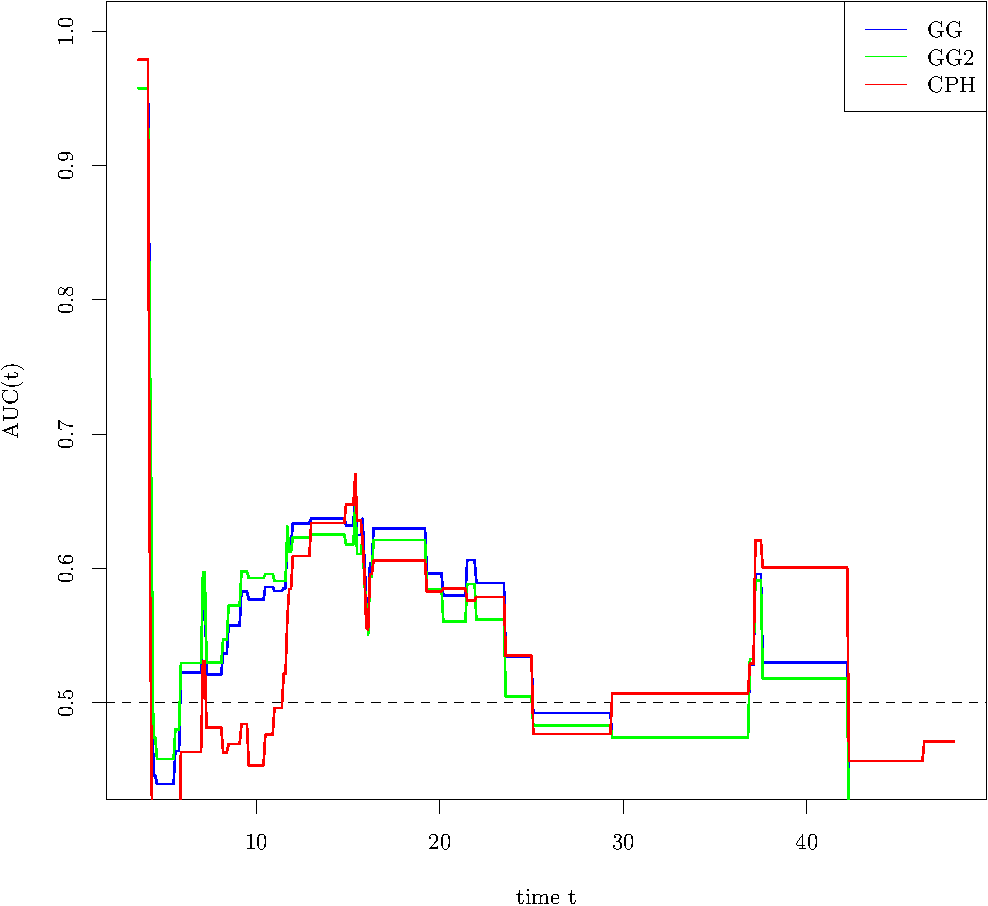
\includegraphics[width=\maxwidth]{figure/05-model-selection-auc-1} 

}



\end{knitrout}


Decision curve analysis.
\begin{knitrout}
\definecolor{shadecolor}{rgb}{0.969, 0.969, 0.969}\color{fgcolor}\begin{kframe}
\begin{alltt}
\hlstd{temp.data} \hlkwb{=} \hlkwd{data.frame}\hlstd{(}\hlkwc{Time} \hlstd{= data.val}\hlopt{$}\hlstd{Time,} \hlkwc{DSD} \hlstd{= data.val}\hlopt{$}\hlstd{DSD}\hlopt{*}\hlnum{1}\hlstd{,}
    \hlkwc{gg.1} \hlstd{=} \hlnum{1}\hlopt{-}\hlstd{val.prob.gg[val.prob.times} \hlopt{==} \hlnum{365}\hlstd{,],} \hlkwc{gg.2} \hlstd{=} \hlnum{1}\hlopt{-}\hlstd{val.prob.gg[val.prob.times} \hlopt{==} \hlnum{365}\hlopt{*}\hlnum{2}\hlstd{,],} \hlkwc{gg.3} \hlstd{=} \hlnum{1}\hlopt{-}\hlstd{val.prob.gg[val.prob.times} \hlopt{==} \hlnum{365}\hlopt{*}\hlnum{3}\hlstd{,],}
    \hlkwc{gg2.1} \hlstd{=} \hlnum{1}\hlopt{-}\hlstd{val.prob.gg2[val.prob.times} \hlopt{==} \hlnum{365}\hlstd{,],} \hlkwc{gg2.2} \hlstd{=} \hlnum{1}\hlopt{-}\hlstd{val.prob.gg2[val.prob.times} \hlopt{==} \hlnum{365}\hlopt{*}\hlnum{2}\hlstd{,],} \hlkwc{gg2.3} \hlstd{=} \hlnum{1}\hlopt{-}\hlstd{val.prob.gg2[val.prob.times} \hlopt{==} \hlnum{365}\hlopt{*}\hlnum{3}\hlstd{,],}
    \hlkwc{cph.1} \hlstd{=} \hlnum{1}\hlopt{-}\hlstd{val.prob.cph[val.prob.times} \hlopt{==} \hlnum{365}\hlstd{,],} \hlkwc{cph.2} \hlstd{=} \hlnum{1}\hlopt{-}\hlstd{val.prob.cph[val.prob.times} \hlopt{==} \hlnum{365}\hlopt{*}\hlnum{2}\hlstd{,],} \hlkwc{cph.3} \hlstd{=} \hlnum{1}\hlopt{-}\hlstd{val.prob.cph[val.prob.times} \hlopt{==} \hlnum{365}\hlopt{*}\hlnum{3}\hlstd{,],}
    \hlkwc{rsf.1} \hlstd{=} \hlnum{1}\hlopt{-}\hlstd{val.prob.rsf[val.prob.times} \hlopt{==} \hlnum{365}\hlstd{,],} \hlkwc{rsf.2} \hlstd{=} \hlnum{1}\hlopt{-}\hlstd{val.prob.rsf[val.prob.times} \hlopt{==} \hlnum{365}\hlopt{*}\hlnum{2}\hlstd{,],} \hlkwc{rsf.3} \hlstd{=} \hlnum{1}\hlopt{-}\hlstd{val.prob.rsf[val.prob.times} \hlopt{==} \hlnum{365}\hlopt{*}\hlnum{3}\hlstd{,])}
\hlkwd{stdca}\hlstd{(}\hlkwc{data} \hlstd{= temp.data,} \hlkwc{outcome} \hlstd{=} \hlstr{"DSD"}\hlstd{,} \hlkwc{ttoutcome} \hlstd{=} \hlstr{"Time"}\hlstd{,} \hlkwc{predictors} \hlstd{=} \hlkwd{c}\hlstd{(}\hlstr{"gg.1"}\hlstd{,} \hlstr{"cph.1"}\hlstd{,} \hlstr{"rsf.1"}\hlstd{),} \hlkwc{timepoint} \hlstd{=} \hlnum{365}\hlstd{,} \hlkwc{probability} \hlstd{=} \hlkwd{rep}\hlstd{(}\hlnum{TRUE}\hlstd{,} \hlnum{3}\hlstd{))}
\end{alltt}
\begin{verbatim}
## [1] "gg.1: No observations with risk greater than 65% that have followup through the timepoint selected, and therefore net benefit not calculable in this range." 
## [2] "cph.1: No observations with risk greater than 69% that have followup through the timepoint selected, and therefore net benefit not calculable in this range."
## [3] "rsf.1: No observations with risk greater than 55% that have followup through the timepoint selected, and therefore net benefit not calculable in this range."
\end{verbatim}
\end{kframe}

{\centering 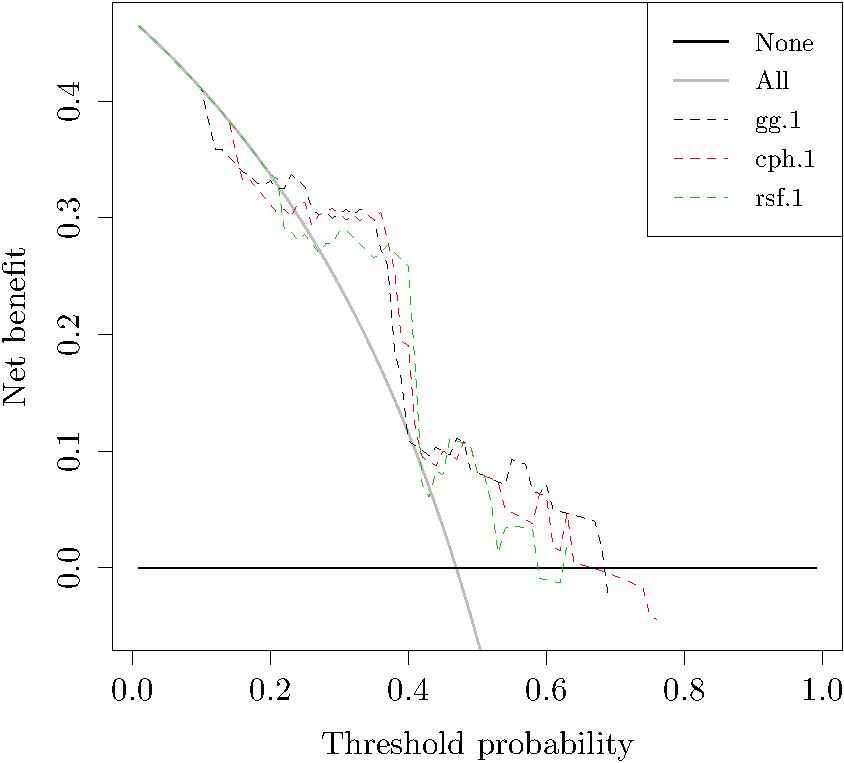
\includegraphics[width=\maxwidth]{figure/05-model-selection-dca-1} 

}


\begin{kframe}\begin{verbatim}
## $N
## [1] 48
## 
## $predictors
##   predictor harm.applied probability
## 1      gg.1            0        TRUE
## 2     cph.1            0        TRUE
## 3     rsf.1            0        TRUE
## 
## $interventions.avoided.per
## [1] 100
## 
## $net.benefit
##    threshold       all none    gg.1   cph.1   rsf.1
## 1       0.01   0.49495    0 0.49495 0.49495 0.49495
## 2       0.02   0.48980    0 0.48980 0.48980 0.48980
## 3       0.03   0.48454    0 0.48454 0.48454 0.48454
## 4       0.04   0.47917    0 0.47917 0.47917 0.47917
## 5       0.05   0.47368    0 0.47368 0.47368 0.47368
## 6       0.06   0.46809    0 0.46809 0.46809 0.46809
## 7       0.07   0.46237    0 0.46237 0.46237 0.46237
## 8       0.08   0.45652    0 0.45652 0.45652 0.45652
## 9       0.09   0.45055    0 0.45055 0.45055 0.45055
## 10      0.10   0.44444    0 0.44444 0.44444 0.44444
## 11      0.11   0.43820    0 0.43820 0.43820 0.43820
## 12      0.12   0.43182    0 0.41098 0.43182 0.43182
## 13      0.13   0.42529    0 0.40445 0.40445 0.42529
## 14      0.14   0.41860    0 0.40455 0.39777 0.41860
## 15      0.15   0.41176    0 0.40196 0.39461 0.41176
## 16      0.16   0.40476    0 0.39583 0.39187 0.40476
## 17      0.17   0.39759    0 0.38956 0.38529 0.39759
## 18      0.18   0.39024    0 0.36687 0.35772 0.39024
## 19      0.19   0.38272    0 0.36060 0.35571 0.38272
## 20      0.20   0.37500    0 0.35417 0.35417 0.37500
## 21      0.21   0.36709    0 0.35311 0.35311 0.36709
## 22      0.22   0.35897    0 0.35844 0.34669 0.34402
## 23      0.23   0.35065    0 0.33171 0.34632 0.34226
## 24      0.24   0.34211    0 0.32566 0.34649 0.34101
## 25      0.25   0.33333    0 0.31944 0.34028 0.33333
## 26      0.26   0.32432    0 0.32038 0.29336 0.33277
## 27      0.27   0.31507    0 0.31421 0.27483 0.33276
## 28      0.28   0.30556    0 0.28704 0.26968 0.34144
## 29      0.29   0.29577    0 0.26438 0.27289 0.32218
## 30      0.30   0.28571    0 0.25893 0.26786 0.30357
## 31      0.31   0.27536    0 0.23249 0.23037 0.29710
## 32      0.32   0.26471    0 0.23652 0.23529 0.26838
## 33      0.33   0.25373    0 0.24129 0.20989 0.24160
## 34      0.34   0.24242    0 0.24684 0.18434 0.21528
## 35      0.35   0.23077    0 0.21154 0.19071 0.22115
## 36      0.36   0.21875    0 0.20703 0.18620 0.21615
## 37      0.37   0.20635    0 0.16071 0.17295 0.20238
## 38      0.38   0.19355    0 0.16868 0.16868 0.16868
## 39      0.39   0.18033    0 0.12261 0.13593 0.16428
## 40      0.40   0.16667    0 0.11111 0.11111 0.15972
## 41      0.41   0.15254    0 0.10699 0.10064 0.16949
## 42      0.42   0.13793    0 0.06106 0.09698 0.12356
## 43      0.43   0.12281    0 0.05154 0.07237 0.10380
## 44      0.44   0.10714    0 0.04762 0.06845 0.10119
## 45      0.45   0.09091    0 0.04356 0.06061 0.11174
## 46      0.46   0.07407    0 0.03935 0.05710 0.11034
## 47      0.47   0.05660    0 0.07193 0.03263 0.08805
## 48      0.48   0.03846    0 0.06891 0.06731 0.06571
## 49      0.49   0.01961    0 0.06577 0.06495 0.08415
## 50      0.50   0.00000    0 0.06250 0.04167 0.06250
## 51      0.51  -0.02041    0 0.05910 0.03912 0.06165
## 52      0.52  -0.04167    0 0.03472 0.03646 0.06076
## 53      0.53  -0.06383    0 0.03103 0.03369 0.05984
## 54      0.54  -0.08696    0 0.05525 0.03080 0.01721
## 55      0.55  -0.11111    0 0.05324 0.02778      NA
## 56      0.56  -0.13636    0 0.05114 0.03030      NA
## 57      0.57  -0.16279    0 0.04893 0.02810      NA
## 58      0.58  -0.19048    0 0.04663 0.02579      NA
## 59      0.59  -0.21951    0 0.04421 0.02337      NA
## 60      0.60  -0.25000    0 0.04167 0.02083      NA
## 61      0.61  -0.28205    0 0.02991 0.01816      NA
## 62      0.62  -0.31579    0 0.02851 0.01535      NA
## 63      0.63  -0.35135    0 0.02703 0.02703      NA
## 64      0.64  -0.38889    0 0.02546 0.02546      NA
## 65      0.65  -0.42857    0      NA 0.02381      NA
## 66      0.66  -0.47059    0      NA 0.02206      NA
## 67      0.67  -0.51515    0      NA 0.02020      NA
## 68      0.68  -0.56250    0      NA 0.01823      NA
## 69      0.69  -0.61290    0      NA      NA      NA
## 70      0.70  -0.66667    0      NA      NA      NA
## 71      0.71  -0.72414    0      NA      NA      NA
## 72      0.72  -0.78571    0      NA      NA      NA
## 73      0.73  -0.85185    0      NA      NA      NA
## 74      0.74  -0.92308    0      NA      NA      NA
## 75      0.75  -1.00000    0      NA      NA      NA
## 76      0.76  -1.08333    0      NA      NA      NA
## 77      0.77  -1.17391    0      NA      NA      NA
## 78      0.78  -1.27273    0      NA      NA      NA
## 79      0.79  -1.38095    0      NA      NA      NA
## 80      0.80  -1.50000    0      NA      NA      NA
## 81      0.81  -1.63158    0      NA      NA      NA
## 82      0.82  -1.77778    0      NA      NA      NA
## 83      0.83  -1.94118    0      NA      NA      NA
## 84      0.84  -2.12500    0      NA      NA      NA
## 85      0.85  -2.33333    0      NA      NA      NA
## 86      0.86  -2.57143    0      NA      NA      NA
## 87      0.87  -2.84615    0      NA      NA      NA
## 88      0.88  -3.16667    0      NA      NA      NA
## 89      0.89  -3.54545    0      NA      NA      NA
## 90      0.90  -4.00000    0      NA      NA      NA
## 91      0.91  -4.55556    0      NA      NA      NA
## 92      0.92  -5.25000    0      NA      NA      NA
## 93      0.93  -6.14286    0      NA      NA      NA
## 94      0.94  -7.33333    0      NA      NA      NA
## 95      0.95  -9.00000    0      NA      NA      NA
## 96      0.96 -11.50000    0      NA      NA      NA
## 97      0.97 -15.66667    0      NA      NA      NA
## 98      0.98 -24.00000    0      NA      NA      NA
## 99      0.99 -49.00000    0      NA      NA      NA
## 
## $interventions.avoided
##    threshold     gg.1   cph.1      rsf.1
## 1       0.01   0.0000   0.000  0.000e+00
## 2       0.02   0.0000   0.000  0.000e+00
## 3       0.03   0.0000   0.000  0.000e+00
## 4       0.04   0.0000   0.000  0.000e+00
## 5       0.05   0.0000   0.000  0.000e+00
## 6       0.06   0.0000   0.000  0.000e+00
## 7       0.07   0.0000   0.000  0.000e+00
## 8       0.08   0.0000   0.000  0.000e+00
## 9       0.09   0.0000   0.000  0.000e+00
## 10      0.10   0.0000   0.000  0.000e+00
## 11      0.11   0.0000   0.000  0.000e+00
## 12      0.12 -15.2778   0.000  0.000e+00
## 13      0.13 -13.9423 -13.942  0.000e+00
## 14      0.14  -8.6310 -12.798  0.000e+00
## 15      0.15  -5.5556  -9.722  0.000e+00
## 16      0.16  -4.6875  -6.771  0.000e+00
## 17      0.17  -3.9216  -6.005  0.000e+00
## 18      0.18 -10.6481 -14.815  0.000e+00
## 19      0.19  -9.4298 -11.513  0.000e+00
## 20      0.20  -8.3333  -8.333  0.000e+00
## 21      0.21  -5.2579  -5.258  0.000e+00
## 22      0.22  -0.1894  -4.356 -5.303e+00
## 23      0.23  -6.3406  -1.449 -2.808e+00
## 24      0.24  -5.2083   1.389 -3.472e-01
## 25      0.25  -4.1667   2.083 -3.331e-14
## 26      0.26  -1.1218  -8.814  2.404e+00
## 27      0.27  -0.2315 -10.880  4.784e+00
## 28      0.28  -4.7619  -9.226  9.226e+00
## 29      0.29  -7.6868  -5.603  6.466e+00
## 30      0.30  -6.2500  -4.167  4.167e+00
## 31      0.31  -9.5430 -10.013  4.839e+00
## 32      0.32  -5.9896  -6.250  7.813e-01
## 33      0.33  -2.5253  -8.902 -2.462e+00
## 34      0.34   0.8578 -11.275 -5.270e+00
## 35      0.35  -3.5714  -7.440 -1.786e+00
## 36      0.36  -2.0833  -5.787 -4.630e-01
## 37      0.37  -7.7703  -5.687 -6.757e-01
## 38      0.38  -4.0570  -4.057 -4.057e+00
## 39      0.39  -9.0278  -6.944 -2.511e+00
## 40      0.40  -8.3333  -8.333 -1.042e+00
## 41      0.41  -6.5549  -7.470  2.439e+00
## 42      0.42 -10.6151  -5.655 -1.984e+00
## 43      0.43  -9.4477  -6.686 -2.519e+00
## 44      0.44  -7.5758  -4.924 -7.576e-01
## 45      0.45  -5.7870  -3.704  2.546e+00
## 46      0.46  -4.0761  -1.993  4.257e+00
## 47      0.47   1.7287  -2.704  3.546e+00
## 48      0.48   3.2986   3.125  2.951e+00
## 49      0.49   4.8044   4.719  6.718e+00
## 50      0.50   6.2500   4.167  6.250e+00
## 51      0.51   7.6389   5.719  7.884e+00
## 52      0.52   7.0513   7.212  9.455e+00
## 53      0.53   8.4119   8.648  1.097e+01
## 54      0.54  12.1142  10.031  8.873e+00
## 55      0.55  13.4470  11.364         NA
## 56      0.56  14.7321  13.095         NA
## 57      0.57  15.9722  14.401         NA
## 58      0.58  17.1695  15.661         NA
## 59      0.59  18.3263  16.879         NA
## 60      0.60  19.4444  18.056         NA
## 61      0.61  19.9454  19.194         NA
## 62      0.62  21.1022  20.296         NA
## 63      0.63  22.2222  22.222         NA
## 64      0.64  23.3073  23.307         NA
## 65      0.65       NA  24.359         NA
## 66      0.66       NA  25.379         NA
## 67      0.67       NA  26.368         NA
## 68      0.68       NA  27.328         NA
## 69      0.69       NA      NA         NA
## 70      0.70       NA      NA         NA
## 71      0.71       NA      NA         NA
## 72      0.72       NA      NA         NA
## 73      0.73       NA      NA         NA
## 74      0.74       NA      NA         NA
## 75      0.75       NA      NA         NA
## 76      0.76       NA      NA         NA
## 77      0.77       NA      NA         NA
## 78      0.78       NA      NA         NA
## 79      0.79       NA      NA         NA
## 80      0.80       NA      NA         NA
## 81      0.81       NA      NA         NA
## 82      0.82       NA      NA         NA
## 83      0.83       NA      NA         NA
## 84      0.84       NA      NA         NA
## 85      0.85       NA      NA         NA
## 86      0.86       NA      NA         NA
## 87      0.87       NA      NA         NA
## 88      0.88       NA      NA         NA
## 89      0.89       NA      NA         NA
## 90      0.90       NA      NA         NA
## 91      0.91       NA      NA         NA
## 92      0.92       NA      NA         NA
## 93      0.93       NA      NA         NA
## 94      0.94       NA      NA         NA
## 95      0.95       NA      NA         NA
## 96      0.96       NA      NA         NA
## 97      0.97       NA      NA         NA
## 98      0.98       NA      NA         NA
## 99      0.99       NA      NA         NA
\end{verbatim}
\begin{alltt}
\hlkwd{stdca}\hlstd{(}\hlkwc{data} \hlstd{= temp.data,} \hlkwc{outcome} \hlstd{=} \hlstr{"DSD"}\hlstd{,} \hlkwc{ttoutcome} \hlstd{=} \hlstr{"Time"}\hlstd{,} \hlkwc{predictors} \hlstd{=} \hlkwd{c}\hlstd{(}\hlstr{"gg.2"}\hlstd{,} \hlstr{"cph.2"}\hlstd{,} \hlstr{"rsf.2"}\hlstd{),} \hlkwc{timepoint} \hlstd{=} \hlnum{365}\hlopt{*}\hlnum{2}\hlstd{,} \hlkwc{probability} \hlstd{=} \hlkwd{rep}\hlstd{(}\hlnum{TRUE}\hlstd{,} \hlnum{3}\hlstd{))}
\end{alltt}
\begin{verbatim}
## [1] "gg.2: No observations with risk greater than 93% that have followup through the timepoint selected, and therefore net benefit not calculable in this range." 
## [2] "cph.2: No observations with risk greater than 91% that have followup through the timepoint selected, and therefore net benefit not calculable in this range."
## [3] "rsf.2: No observations with risk greater than 74% that have followup through the timepoint selected, and therefore net benefit not calculable in this range."
\end{verbatim}
\end{kframe}

{\centering 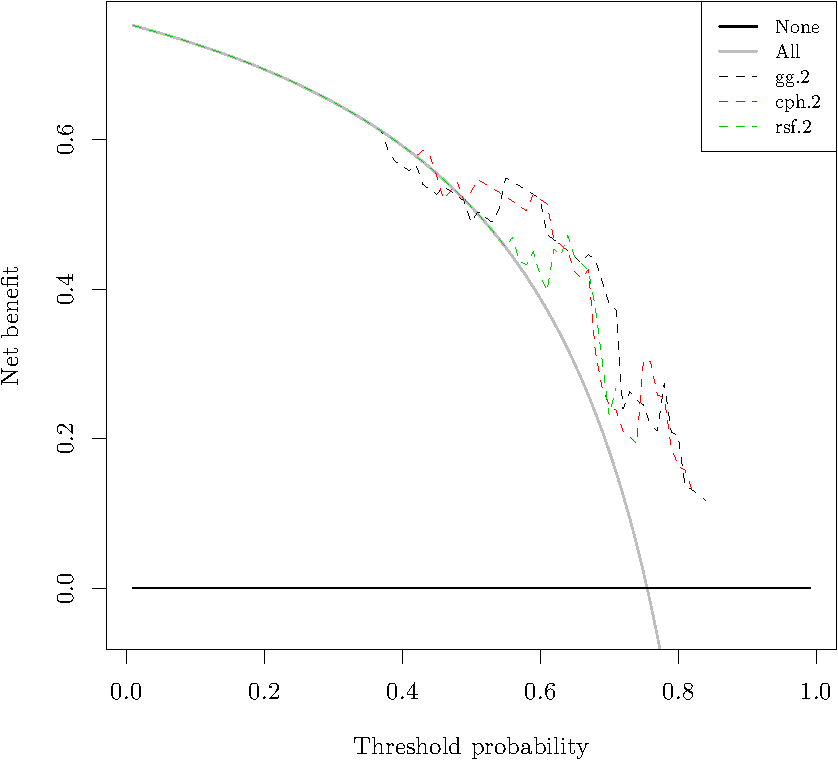
\includegraphics[width=\maxwidth]{figure/05-model-selection-dca-2} 

}


\begin{kframe}\begin{verbatim}
## $N
## [1] 48
## 
## $predictors
##   predictor harm.applied probability
## 1      gg.2            0        TRUE
## 2     cph.2            0        TRUE
## 3     rsf.2            0        TRUE
## 
## $interventions.avoided.per
## [1] 100
## 
## $net.benefit
##    threshold        all none     gg.2    cph.2   rsf.2
## 1       0.01   0.797078    0  0.79708  0.79708 0.79708
## 2       0.02   0.795007    0  0.79501  0.79501 0.79501
## 3       0.03   0.792894    0  0.79289  0.79289 0.79289
## 4       0.04   0.790737    0  0.79074  0.79074 0.79074
## 5       0.05   0.788534    0  0.78853  0.78853 0.78853
## 6       0.06   0.786284    0  0.78628  0.78628 0.78628
## 7       0.07   0.783986    0  0.78399  0.78399 0.78399
## 8       0.08   0.781638    0  0.78164  0.78164 0.78164
## 9       0.09   0.779239    0  0.77924  0.77924 0.77924
## 10      0.10   0.776786    0  0.77679  0.77679 0.77679
## 11      0.11   0.774278    0  0.77428  0.77428 0.77428
## 12      0.12   0.771713    0  0.77171  0.77171 0.77171
## 13      0.13   0.769089    0  0.76909  0.76909 0.76909
## 14      0.14   0.766404    0  0.76640  0.76640 0.76640
## 15      0.15   0.763655    0  0.76366  0.76366 0.76366
## 16      0.16   0.760842    0  0.76084  0.76084 0.76084
## 17      0.17   0.757960    0  0.75796  0.75796 0.75796
## 18      0.18   0.755009    0  0.75501  0.75501 0.75501
## 19      0.19   0.751984    0  0.75198  0.75198 0.75198
## 20      0.20   0.748884    0  0.74888  0.74888 0.74888
## 21      0.21   0.745705    0  0.74571  0.74571 0.74571
## 22      0.22   0.742445    0  0.74245  0.74245 0.74245
## 23      0.23   0.739100    0  0.73910  0.73910 0.73910
## 24      0.24   0.735667    0  0.73567  0.73567 0.73567
## 25      0.25   0.732143    0  0.73214  0.73214 0.73214
## 26      0.26   0.728523    0  0.72852  0.72852 0.72852
## 27      0.27   0.724804    0  0.72480  0.72480 0.72480
## 28      0.28   0.720982    0  0.72098  0.72098 0.72098
## 29      0.29   0.717052    0  0.71705  0.71705 0.71705
## 30      0.30   0.713010    0  0.71301  0.71301 0.71301
## 31      0.31   0.708851    0  0.70885  0.70885 0.70885
## 32      0.32   0.704569    0  0.70457  0.70457 0.70457
## 33      0.33   0.700160    0  0.70016  0.70016 0.70016
## 34      0.34   0.695617    0  0.67478  0.69562 0.69562
## 35      0.35   0.690934    0  0.67010  0.69093 0.69093
## 36      0.36   0.686105    0  0.66527  0.68610 0.68610
## 37      0.37   0.681122    0  0.66029  0.68112 0.68112
## 38      0.38   0.675979    0  0.65515  0.68967 0.67598
## 39      0.39   0.670667    0  0.62900  0.68493 0.67067
## 40      0.40   0.665179    0  0.62351  0.68002 0.66518
## 41      0.41   0.659504    0  0.61064  0.67495 0.65950
## 42      0.42   0.653633    0  0.60536  0.66971 0.65363
## 43      0.43   0.647556    0  0.59990  0.64344 0.64756
## 44      0.44   0.641263    0  0.59425  0.61699 0.64126
## 45      0.45   0.634740    0  0.58838  0.61116 0.63474
## 46      0.46   0.627976    0  0.58230  0.60512 0.62798
## 47      0.47   0.620957    0  0.55516  0.59884 0.62096
## 48      0.48   0.613668    0  0.52778  0.57150 0.61367
## 49      0.49   0.606092    0  0.52097  0.56306 0.60609
## 50      0.50   0.598214    0  0.51389  0.53598 0.59821
## 51      0.51   0.590015    0  0.50652  0.52949 0.59001
## 52      0.52   0.581473    0  0.49884  0.52273 0.58147
## 53      0.53   0.572568    0  0.51568  0.49484 0.57257
## 54      0.54   0.563276    0  0.46665  0.48748 0.56814
## 55      0.55   0.553571    0  0.45896  0.47980 0.53864
## 56      0.56   0.543425    0  0.45093  0.47176 0.53426
## 57      0.57   0.532807    0  0.41860  0.46335 0.52585
## 58      0.58   0.521684    0  0.40972  0.43371 0.49621
## 59      0.59   0.510017    0  0.40041  0.40364 0.48697
## 60      0.60   0.497768    0  0.39062  0.39394 0.45644
## 61      0.61   0.484890    0  0.38034  0.39387 0.48077
## 62      0.62   0.471335    0  0.36952  0.38450 0.47149
## 63      0.63   0.457046    0  0.39546  0.37462 0.42005
## 64      0.64   0.441964    0  0.36420  0.36420 0.40972
## 65      0.65   0.426020    0  0.35317  0.35317 0.39881
## 66      0.66   0.409139    0  0.38450  0.34283 0.36642
## 67      0.67   0.391234    0  0.35322  0.31155 0.37405
## 68      0.68   0.372210    0  0.22439  0.27962 0.36296
## 69      0.69   0.351959    0  0.21214  0.19931 0.38028
## 70      0.70   0.330357    0  0.15741  0.06250 0.28009
## 71      0.71   0.307266    0  0.12261  0.02730 0.24593
## 72      0.72   0.282526    0  0.14286  0.01190 0.04762
## 73      0.73   0.255952    0  0.07253 -0.00463 0.07485
## 74      0.74   0.227335    0  0.05769  0.03686      NA
## 75      0.75   0.196429    0  0.06250  0.02083      NA
## 76      0.76   0.162946    0  0.04861 -0.01736      NA
## 77      0.77   0.126553    0 -0.02899  0.10326      NA
## 78      0.78   0.086851    0 -0.04545  0.10227      NA
## 79      0.79   0.043367    0  0.09325  0.09325      NA
## 80      0.80  -0.004464    0  0.08333  0.08333      NA
## 81      0.81  -0.057331    0  0.05154  0.05154      NA
## 82      0.82  -0.116071    0  0.03935  0.03935      NA
## 83      0.83  -0.181723    0  0.02574  0.02574      NA
## 84      0.84  -0.255580    0 -0.03125 -0.07292      NA
## 85      0.85  -0.339286    0 -0.09028 -0.09028      NA
## 86      0.86  -0.434949    0 -0.11012 -0.11012      NA
## 87      0.87  -0.545330    0 -0.13301 -0.13301      NA
## 88      0.88  -0.674107    0 -0.02778 -0.15972      NA
## 89      0.89  -0.826299    0 -0.04356 -0.04356      NA
## 90      0.90  -1.008929    0 -0.08333 -0.06250      NA
## 91      0.91  -1.232143    0 -0.14815       NA      NA
## 92      0.92  -1.511161    0 -0.19792       NA      NA
## 93      0.93  -1.869898    0       NA       NA      NA
## 94      0.94  -2.348214    0       NA       NA      NA
## 95      0.95  -3.017857    0       NA       NA      NA
## 96      0.96  -4.022321    0       NA       NA      NA
## 97      0.97  -5.696429    0       NA       NA      NA
## 98      0.98  -9.044643    0       NA       NA      NA
## 99      0.99 -19.089286    0       NA       NA      NA
## 
## $interventions.avoided
##    threshold   gg.2    cph.2     rsf.2
## 1       0.01  0.000   0.0000  0.000000
## 2       0.02  0.000   0.0000  0.000000
## 3       0.03  0.000   0.0000  0.000000
## 4       0.04  0.000   0.0000  0.000000
## 5       0.05  0.000   0.0000  0.000000
## 6       0.06  0.000   0.0000  0.000000
## 7       0.07  0.000   0.0000  0.000000
## 8       0.08  0.000   0.0000  0.000000
## 9       0.09  0.000   0.0000  0.000000
## 10      0.10  0.000   0.0000  0.000000
## 11      0.11  0.000   0.0000  0.000000
## 12      0.12  0.000   0.0000  0.000000
## 13      0.13  0.000   0.0000  0.000000
## 14      0.14  0.000   0.0000  0.000000
## 15      0.15  0.000   0.0000  0.000000
## 16      0.16  0.000   0.0000  0.000000
## 17      0.17  0.000   0.0000  0.000000
## 18      0.18  0.000   0.0000  0.000000
## 19      0.19  0.000   0.0000  0.000000
## 20      0.20  0.000   0.0000  0.000000
## 21      0.21  0.000   0.0000  0.000000
## 22      0.22  0.000   0.0000  0.000000
## 23      0.23  0.000   0.0000  0.000000
## 24      0.24  0.000   0.0000  0.000000
## 25      0.25  0.000   0.0000  0.000000
## 26      0.26  0.000   0.0000  0.000000
## 27      0.27  0.000   0.0000  0.000000
## 28      0.28  0.000   0.0000  0.000000
## 29      0.29  0.000   0.0000  0.000000
## 30      0.30  0.000   0.0000  0.000000
## 31      0.31  0.000   0.0000  0.000000
## 32      0.32  0.000   0.0000  0.000000
## 33      0.33  0.000   0.0000  0.000000
## 34      0.34 -4.044   0.0000  0.000000
## 35      0.35 -3.869   0.0000  0.000000
## 36      0.36 -3.704   0.0000  0.000000
## 37      0.37 -3.547   0.0000  0.000000
## 38      0.38 -3.399   2.2340  0.000000
## 39      0.39 -6.517   2.2301  0.000000
## 40      0.40 -6.250   2.2264  0.000000
## 41      0.41 -7.032   2.2229  0.000000
## 42      0.42 -6.666   2.2196  0.000000
## 43      0.43 -6.317  -0.5452  0.000000
## 44      0.44 -5.984  -3.0896  0.000000
## 45      0.45 -5.666  -2.8821  0.000000
## 46      0.46 -5.361  -2.6835  0.000000
## 47      0.47 -7.419  -2.4935  0.000000
## 48      0.48 -9.305  -4.5683  0.000000
## 49      0.49 -8.860  -4.4792  0.000000
## 50      0.50 -8.433  -6.2229  0.000000
## 51      0.51 -8.022  -5.8150  0.000000
## 52      0.52 -7.627  -5.4227  0.000000
## 53      0.53 -5.045  -6.8927  0.000000
## 54      0.54 -8.231  -6.4564  0.414632
## 55      0.55 -7.741  -6.0360 -1.221695
## 56      0.56 -7.268  -5.6306 -0.719890
## 57      0.57 -8.615  -5.2394 -0.524512
## 58      0.58 -8.108  -6.3704 -1.844492
## 59      0.59 -7.617  -7.3923 -1.601365
## 60      0.60 -7.143  -6.9219 -2.755231
## 61      0.61 -6.684  -5.8190 -0.263466
## 62      0.62 -6.240  -5.3219  0.009601
## 63      0.63 -3.617  -4.8406 -2.173091
## 64      0.64 -4.374  -4.3744 -1.813616
## 65      0.65 -3.922  -3.9225 -1.465201
## 66      0.66 -1.269  -3.4159 -2.200577
## 67      0.67 -1.872  -3.9246 -0.846215
## 68      0.68 -6.956  -4.3571 -0.435487
## 69      0.69 -6.282  -6.8582  1.272429
## 70      0.70 -7.412 -11.4796 -2.154195
## 71      0.71 -7.542 -11.4353 -2.505310
## 72      0.72 -5.432 -10.5241 -9.135251
## 73      0.73 -6.784  -9.6380 -6.698467
## 74      0.74 -5.960  -6.6924        NA
## 75      0.75 -4.464  -5.8532        NA
## 76      0.76 -3.611  -5.6939        NA
## 77      0.77 -4.646  -0.6957        NA
## 78      0.78 -3.732   0.4350        NA
## 79      0.79  1.326   1.3261        NA
## 80      0.80  2.195   2.1949        NA
## 81      0.81  2.554   2.5536        NA
## 82      0.82  3.412   3.4117        NA
## 83      0.83  4.249   4.2491        NA
## 84      0.84  4.273   3.4793        NA
## 85      0.85  4.394   4.3943        NA
## 86      0.86  5.288   5.2879        NA
## 87      0.87  6.161   6.1611        NA
## 88      0.88  8.814   7.0143        NA
## 89      0.89  9.674   9.6743        NA
## 90      0.90 10.284  10.5159        NA
## 91      0.91 10.721       NA        NA
## 92      0.92 11.420       NA        NA
## 93      0.93     NA       NA        NA
## 94      0.94     NA       NA        NA
## 95      0.95     NA       NA        NA
## 96      0.96     NA       NA        NA
## 97      0.97     NA       NA        NA
## 98      0.98     NA       NA        NA
## 99      0.99     NA       NA        NA
\end{verbatim}
\begin{alltt}
\hlkwd{stdca}\hlstd{(}\hlkwc{data} \hlstd{= temp.data,} \hlkwc{outcome} \hlstd{=} \hlstr{"DSD"}\hlstd{,} \hlkwc{ttoutcome} \hlstd{=} \hlstr{"Time"}\hlstd{,} \hlkwc{predictors} \hlstd{=} \hlkwd{c}\hlstd{(}\hlstr{"gg.3"}\hlstd{,} \hlstr{"cph.3"}\hlstd{,} \hlstr{"rsf.3"}\hlstd{),} \hlkwc{timepoint} \hlstd{=} \hlnum{365}\hlopt{*}\hlnum{3}\hlstd{,} \hlkwc{probability} \hlstd{=} \hlkwd{rep}\hlstd{(}\hlnum{TRUE}\hlstd{,} \hlnum{3}\hlstd{))}
\end{alltt}
\begin{verbatim}
## [1] "rsf.3: No observations with risk greater than 90% that have followup through the timepoint selected, and therefore net benefit not calculable in this range."
\end{verbatim}
\end{kframe}

{\centering 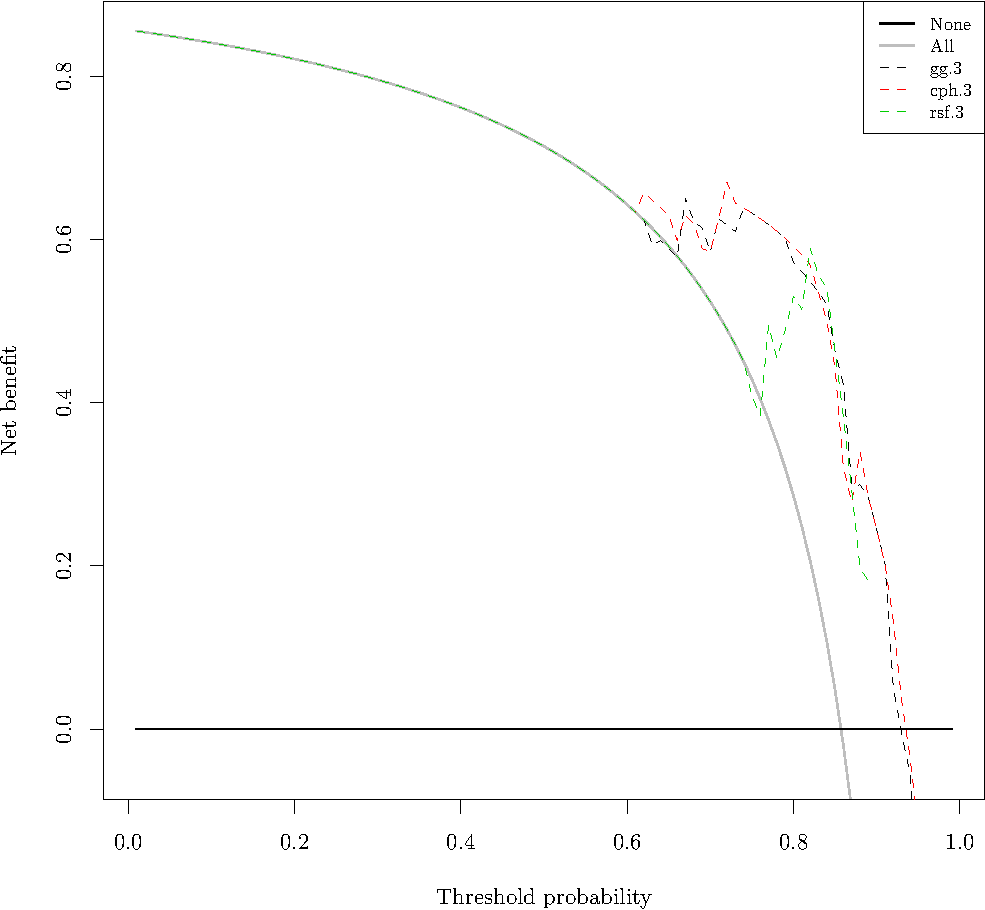
\includegraphics[width=\maxwidth]{figure/05-model-selection-dca-3} 

}


\begin{kframe}\begin{verbatim}
## $N
## [1] 48
## 
## $predictors
##   predictor harm.applied probability
## 1      gg.3            0        TRUE
## 2     cph.3            0        TRUE
## 3     rsf.3            0        TRUE
## 
## $interventions.avoided.per
## [1] 100
## 
## $net.benefit
##    threshold       all none     gg.3     cph.3     rsf.3
## 1       0.01   0.84217    0  0.84217  0.842172  0.842172
## 2       0.02   0.84056    0  0.84056  0.840561  0.840561
## 3       0.03   0.83892    0  0.83892  0.838918  0.838918
## 4       0.04   0.83724    0  0.83724  0.837240  0.837240
## 5       0.05   0.83553    0  0.83553  0.835526  0.835526
## 6       0.06   0.83378    0  0.83378  0.833777  0.833777
## 7       0.07   0.83199    0  0.83199  0.831989  0.831989
## 8       0.08   0.83016    0  0.83016  0.830163  0.830163
## 9       0.09   0.82830    0  0.82830  0.828297  0.828297
## 10      0.10   0.82639    0  0.82639  0.826389  0.826389
## 11      0.11   0.82444    0  0.82444  0.824438  0.824438
## 12      0.12   0.82244    0  0.82244  0.822443  0.822443
## 13      0.13   0.82040    0  0.82040  0.820402  0.820402
## 14      0.14   0.81831    0  0.81831  0.818314  0.818314
## 15      0.15   0.81618    0  0.81618  0.816176  0.816176
## 16      0.16   0.81399    0  0.81399  0.813988  0.813988
## 17      0.17   0.81175    0  0.81175  0.811747  0.811747
## 18      0.18   0.80945    0  0.80945  0.809451  0.809451
## 19      0.19   0.80710    0  0.80710  0.807099  0.807099
## 20      0.20   0.80469    0  0.80469  0.804688  0.804688
## 21      0.21   0.80222    0  0.80222  0.802215  0.802215
## 22      0.22   0.79968    0  0.79968  0.799679  0.799679
## 23      0.23   0.79708    0  0.79708  0.797078  0.797078
## 24      0.24   0.79441    0  0.79441  0.794408  0.794408
## 25      0.25   0.79167    0  0.79167  0.791667  0.791667
## 26      0.26   0.78885    0  0.78885  0.788851  0.788851
## 27      0.27   0.78596    0  0.78596  0.785959  0.785959
## 28      0.28   0.78299    0  0.78299  0.782986  0.782986
## 29      0.29   0.77993    0  0.77993  0.779930  0.779930
## 30      0.30   0.77679    0  0.77679  0.776786  0.776786
## 31      0.31   0.77355    0  0.77355  0.773551  0.773551
## 32      0.32   0.77022    0  0.77022  0.770221  0.770221
## 33      0.33   0.76679    0  0.76679  0.766791  0.766791
## 34      0.34   0.76326    0  0.76326  0.763258  0.763258
## 35      0.35   0.75962    0  0.75962  0.759615  0.759615
## 36      0.36   0.75586    0  0.75586  0.755859  0.755859
## 37      0.37   0.75198    0  0.75198  0.751984  0.751984
## 38      0.38   0.74798    0  0.74798  0.747984  0.747984
## 39      0.39   0.74385    0  0.74385  0.743852  0.743852
## 40      0.40   0.73958    0  0.73958  0.739583  0.739583
## 41      0.41   0.73517    0  0.73517  0.735169  0.735169
## 42      0.42   0.73060    0  0.73060  0.730603  0.730603
## 43      0.43   0.72588    0  0.72588  0.725877  0.725877
## 44      0.44   0.72098    0  0.72098  0.720982  0.720982
## 45      0.45   0.71591    0  0.71591  0.715909  0.715909
## 46      0.46   0.71065    0  0.71065  0.710648  0.710648
## 47      0.47   0.70519    0  0.70519  0.705189  0.705189
## 48      0.48   0.69952    0  0.69952  0.699519  0.699519
## 49      0.49   0.69363    0  0.69363  0.693627  0.693627
## 50      0.50   0.68750    0  0.68750  0.687500  0.687500
## 51      0.51   0.68112    0  0.68112  0.681122  0.681122
## 52      0.52   0.67448    0  0.67448  0.674479  0.674479
## 53      0.53   0.66755    0  0.66755  0.667553  0.667553
## 54      0.54   0.66033    0  0.66033  0.660326  0.660326
## 55      0.55   0.65278    0  0.65278  0.680021  0.652778
## 56      0.56   0.64489    0  0.64489  0.673223  0.644886
## 57      0.57   0.63663    0  0.61579  0.666108  0.636628
## 58      0.58   0.62798    0  0.60714  0.658654  0.627976
## 59      0.59   0.61890    0  0.59807  0.650836  0.618902
## 60      0.60   0.60938    0  0.58854  0.642628  0.609375
## 61      0.61   0.59936    0  0.61317  0.633999  0.599359
## 62      0.62   0.58882    0  0.60408  0.604082  0.588816
## 63      0.63   0.57770    0  0.59451  0.594508  0.577703
## 64      0.64   0.56597    0  0.56357  0.584402  0.565972
## 65      0.65   0.55357    0  0.52976  0.573718  0.553571
## 66      0.66   0.54044    0  0.51838  0.562406  0.540441
## 67      0.67   0.52652    0  0.48548  0.550408  0.526515
## 68      0.68   0.51172    0  0.47266  0.493490  0.511719
## 69      0.69   0.49597    0  0.45901  0.459005  0.495968
## 70      0.70   0.47917    0  0.44444  0.444444  0.458333
## 71      0.71   0.46121    0  0.42888  0.428879  0.440374
## 72      0.72   0.44196    0  0.36715  0.412202  0.421131
## 73      0.73   0.42130    0  0.32828  0.394290  0.376662
## 74      0.74   0.39904    0  0.30886  0.354167  0.354290
## 75      0.75   0.37500    0  0.28788  0.308712  0.395833
## 76      0.76   0.34896    0  0.26515  0.285985  0.331597
## 77      0.77   0.32065    0  0.24045  0.240448  0.307065
## 78      0.78   0.28977    0  0.21350  0.213499  0.255165
## 79      0.79   0.25595    0  0.16315  0.163149  0.225649
## 80      0.80   0.21875    0  0.10985  0.218750  0.193182
## 81      0.81   0.17763    0  0.07396  0.188596  0.136463
## 82      0.82   0.13194    0  0.10700  0.155093  0.096591
## 83      0.83   0.08088    0  0.06917  0.117647  0.052028
## 84      0.84   0.02344    0  0.02662 -0.007813 -0.046875
## 85      0.85  -0.04167    0 -0.06327 -0.104938 -0.125000
## 86      0.86  -0.11607    0 -0.16005 -0.212054 -0.160053
## 87      0.87  -0.20192    0 -0.12843 -0.276442 -0.244480
## 88      0.88  -0.30208    0 -0.23115 -0.372396 -0.145833
## 89      0.89  -0.42045    0 -0.30330 -0.282468  0.007576
## 90      0.90  -0.56250    0 -0.56250 -0.369048        NA
## 91      0.91  -0.73611    0 -0.29861 -0.194444        NA
## 92      0.92  -0.95313    0 -0.38542 -0.385417        NA
## 93      0.93  -1.23214    0 -0.26190 -0.497024        NA
## 94      0.94  -1.60417    0 -0.38194 -0.319444        NA
## 95      0.95  -2.12500    0 -0.58333 -0.500000        NA
## 96      0.96  -2.90625    0 -0.31250 -0.791667        NA
## 97      0.97  -4.20833    0 -0.56944 -1.159722        NA
## 98      0.98  -6.81250    0 -0.97917 -0.895833        NA
## 99      0.99 -14.62500    0 -2.02083 -1.979167        NA
## 
## $interventions.avoided
##    threshold       gg.3      cph.3   rsf.3
## 1       0.01  0.000e+00  0.000e+00  0.0000
## 2       0.02  0.000e+00  0.000e+00  0.0000
## 3       0.03  0.000e+00  0.000e+00  0.0000
## 4       0.04  0.000e+00  0.000e+00  0.0000
## 5       0.05  0.000e+00  0.000e+00  0.0000
## 6       0.06  0.000e+00  0.000e+00  0.0000
## 7       0.07  0.000e+00  0.000e+00  0.0000
## 8       0.08  0.000e+00  0.000e+00  0.0000
## 9       0.09  0.000e+00  0.000e+00  0.0000
## 10      0.10  0.000e+00  0.000e+00  0.0000
## 11      0.11  0.000e+00  0.000e+00  0.0000
## 12      0.12  0.000e+00  0.000e+00  0.0000
## 13      0.13  0.000e+00  0.000e+00  0.0000
## 14      0.14  0.000e+00  0.000e+00  0.0000
## 15      0.15  0.000e+00  0.000e+00  0.0000
## 16      0.16  0.000e+00  0.000e+00  0.0000
## 17      0.17  0.000e+00  0.000e+00  0.0000
## 18      0.18  0.000e+00  0.000e+00  0.0000
## 19      0.19  0.000e+00  0.000e+00  0.0000
## 20      0.20  0.000e+00  0.000e+00  0.0000
## 21      0.21  0.000e+00  0.000e+00  0.0000
## 22      0.22  0.000e+00  0.000e+00  0.0000
## 23      0.23  0.000e+00  0.000e+00  0.0000
## 24      0.24  0.000e+00  0.000e+00  0.0000
## 25      0.25  0.000e+00  0.000e+00  0.0000
## 26      0.26  0.000e+00  0.000e+00  0.0000
## 27      0.27  0.000e+00  0.000e+00  0.0000
## 28      0.28  0.000e+00  0.000e+00  0.0000
## 29      0.29  0.000e+00  0.000e+00  0.0000
## 30      0.30  0.000e+00  0.000e+00  0.0000
## 31      0.31  0.000e+00  0.000e+00  0.0000
## 32      0.32  0.000e+00  0.000e+00  0.0000
## 33      0.33  0.000e+00  0.000e+00  0.0000
## 34      0.34  0.000e+00  0.000e+00  0.0000
## 35      0.35  0.000e+00  0.000e+00  0.0000
## 36      0.36  0.000e+00  0.000e+00  0.0000
## 37      0.37  0.000e+00  0.000e+00  0.0000
## 38      0.38  0.000e+00  0.000e+00  0.0000
## 39      0.39  0.000e+00  0.000e+00  0.0000
## 40      0.40  0.000e+00  0.000e+00  0.0000
## 41      0.41  0.000e+00  0.000e+00  0.0000
## 42      0.42  0.000e+00  0.000e+00  0.0000
## 43      0.43  0.000e+00  0.000e+00  0.0000
## 44      0.44  0.000e+00  0.000e+00  0.0000
## 45      0.45  0.000e+00  0.000e+00  0.0000
## 46      0.46  0.000e+00  0.000e+00  0.0000
## 47      0.47  0.000e+00  0.000e+00  0.0000
## 48      0.48  0.000e+00  0.000e+00  0.0000
## 49      0.49  0.000e+00  0.000e+00  0.0000
## 50      0.50  0.000e+00  0.000e+00  0.0000
## 51      0.51  0.000e+00  0.000e+00  0.0000
## 52      0.52  0.000e+00  0.000e+00  0.0000
## 53      0.53  0.000e+00  0.000e+00  0.0000
## 54      0.54  0.000e+00  0.000e+00  0.0000
## 55      0.55  0.000e+00  2.229e+00  0.0000
## 56      0.56  0.000e+00  2.226e+00  0.0000
## 57      0.57 -1.572e+00  2.224e+00  0.0000
## 58      0.58 -1.509e+00  2.221e+00  0.0000
## 59      0.59 -1.448e+00  2.219e+00  0.0000
## 60      0.60 -1.389e+00  2.217e+00  0.0000
## 61      0.61  8.827e-01  2.215e+00  0.0000
## 62      0.62  9.357e-01  9.357e-01  0.0000
## 63      0.63  9.870e-01  9.870e-01  0.0000
## 64      0.64 -1.352e-01  1.037e+00  0.0000
## 65      0.65 -1.282e+00  1.085e+00  0.0000
## 66      0.66 -1.136e+00  1.132e+00  0.0000
## 67      0.67 -2.021e+00  1.177e+00  0.0000
## 68      0.68 -1.838e+00 -8.578e-01  0.0000
## 69      0.69 -1.661e+00 -1.661e+00  0.0000
## 70      0.70 -1.488e+00 -1.488e+00 -0.8929
## 71      0.71 -1.320e+00 -1.320e+00 -0.8509
## 72      0.72 -2.909e+00 -1.157e+00 -0.8102
## 73      0.73 -3.440e+00 -9.989e-01 -1.6509
## 74      0.74 -3.169e+00 -1.577e+00 -1.5722
## 75      0.75 -2.904e+00 -2.210e+00  0.6944
## 76      0.76 -2.647e+00 -1.989e+00 -0.5482
## 77      0.77 -2.396e+00 -2.396e+00 -0.4058
## 78      0.78 -2.151e+00 -2.151e+00 -0.9761
## 79      0.79 -2.467e+00 -2.467e+00 -0.8055
## 80      0.80 -2.723e+00 -2.776e-15 -0.6392
## 81      0.81 -2.432e+00  2.572e-01 -0.9657
## 82      0.82 -5.477e-01  5.081e-01 -0.7761
## 83      0.83 -2.398e-01  7.530e-01 -0.5910
## 84      0.84  6.063e-02 -5.952e-01 -1.3393
## 85      0.85 -3.813e-01 -1.117e+00 -1.4706
## 86      0.86 -7.160e-01 -1.563e+00 -0.7160
## 87      0.87  1.098e+00 -1.114e+00 -0.6359
## 88      0.88  9.673e-01 -9.588e-01  2.1307
## 89      0.89  1.448e+00  1.705e+00  5.2903
## 90      0.90  2.467e-15  2.149e+00      NA
## 91      0.91  4.327e+00  5.357e+00      NA
## 92      0.92  4.937e+00  4.937e+00      NA
## 93      0.93  7.303e+00  5.533e+00      NA
## 94      0.94  7.801e+00  8.200e+00      NA
## 95      0.95  8.114e+00  8.553e+00      NA
## 96      0.96  1.081e+01  8.811e+00      NA
## 97      0.97  1.125e+01  9.429e+00      NA
## 98      0.98  1.190e+01  1.207e+01      NA
## 99      0.99  1.273e+01  1.277e+01      NA
\end{verbatim}
\end{kframe}
\end{knitrout}


Evaluate IBS point estimates.
BS paths over time on bootstrap samples of the holdout set.
\begin{knitrout}
\definecolor{shadecolor}{rgb}{0.969, 0.969, 0.969}\color{fgcolor}\begin{kframe}
\begin{alltt}
\hlkwd{set.seed}\hlstd{(}\hlnum{20150111}\hlstd{)}
\hlstd{ibs_eval_times} \hlkwb{=} \hlkwd{calcIBS}\hlstd{(}\hlkwd{Surv}\hlstd{(data.val}\hlopt{$}\hlstd{Time, data.val}\hlopt{$}\hlstd{DSD), ibs_preds_gg, ibs_times,} \hlkwd{max}\hlstd{(data.val}\hlopt{$}\hlstd{Time))}\hlopt{$}\hlstd{eval_times}
\hlcom{# bsc_boot2 = lapply(ibs_preds_all, function(preds) boot(data.val, statistic = function(d, i) calcIBS(Surv(d$Time, d$DSD)[i,], preds[i,], ibs_times, max(d$Time))$bsc, R = 500))}
\hlcom{# bsc_boot2ci = lapply(bsc_boot2, function(single_boot) t(sapply(1:length(ibs_eval_times), function(time_index) \{}
\hlcom{# 	temp = try(boot.ci(single_boot, index = time_index, type = "bca")$bca, silent = TRUE)}
\hlcom{# 	if (class(temp) == "try-error" || is.null(temp)) \{ temp = rep(NA, 5) \}}
\hlcom{# 	temp \})))}
\hlstd{bsc_boots} \hlkwb{=} \hlkwd{laply}\hlstd{(}\hlnum{1}\hlopt{:}\hlnum{500}\hlstd{,} \hlkwa{function}\hlstd{(}\hlkwc{i}\hlstd{) \{}
        \hlkwa{if} \hlstd{(i} \hlopt \hlnum{50} \hlopt{==} \hlnum{0}\hlstd{)       \{} \hlkwd{message}\hlstd{(i) \}}
        \hlstd{boot_samp} \hlkwb{=} \hlkwd{sample.int}\hlstd{(}\hlkwd{nrow}\hlstd{(data.val),} \hlkwc{replace} \hlstd{=} \hlnum{TRUE}\hlstd{)}
        \hlstd{gg} \hlkwb{=} \hlkwd{calcIBS}\hlstd{(}\hlkwd{Surv}\hlstd{(data.val}\hlopt{$}\hlstd{Time, data.val}\hlopt{$}\hlstd{DSD)[boot_samp,], ibs_preds_gg[boot_samp,], ibs_times,} \hlkwd{max}\hlstd{(data.val}\hlopt{$}\hlstd{Time))}\hlopt{$}\hlstd{bsc}
        \hlstd{gg2} \hlkwb{=} \hlkwd{calcIBS}\hlstd{(}\hlkwd{Surv}\hlstd{(data.val}\hlopt{$}\hlstd{Time, data.val}\hlopt{$}\hlstd{DSD)[boot_samp,], ibs_preds_gg2[boot_samp,], ibs_times,} \hlkwd{max}\hlstd{(data.val}\hlopt{$}\hlstd{Time))}\hlopt{$}\hlstd{bsc}
        \hlstd{cph} \hlkwb{=} \hlkwd{calcIBS}\hlstd{(}\hlkwd{Surv}\hlstd{(data.val}\hlopt{$}\hlstd{Time, data.val}\hlopt{$}\hlstd{DSD)[boot_samp,], ibs_preds_cph[boot_samp,], ibs_times,} \hlkwd{max}\hlstd{(data.val}\hlopt{$}\hlstd{Time))}\hlopt{$}\hlstd{bsc}
        \hlstd{rsf} \hlkwb{=} \hlkwd{calcIBS}\hlstd{(}\hlkwd{Surv}\hlstd{(data.val}\hlopt{$}\hlstd{Time, data.val}\hlopt{$}\hlstd{DSD)[boot_samp,], ibs_preds_rsf[boot_samp,], ibs_times,} \hlkwd{max}\hlstd{(data.val}\hlopt{$}\hlstd{Time))}\hlopt{$}\hlstd{bsc}
        \hlstd{km0} \hlkwb{=} \hlkwd{calcIBS}\hlstd{(}\hlkwd{Surv}\hlstd{(data.val}\hlopt{$}\hlstd{Time, data.val}\hlopt{$}\hlstd{DSD)[boot_samp,], ibs_preds_km0[boot_samp,], ibs_times,} \hlkwd{max}\hlstd{(data.val}\hlopt{$}\hlstd{Time))}\hlopt{$}\hlstd{bsc}
        \hlkwd{rbind}\hlstd{(gg, gg2, cph, rsf, km0)}
\hlstd{\})}
\end{alltt}


{\ttfamily\noindent\itshape\color{messagecolor}{\#\# 50\\\#\# 100\\\#\# 150\\\#\# 200\\\#\# 250\\\#\# 300\\\#\# 350\\\#\# 400\\\#\# 450\\\#\# 500}}\end{kframe}
\end{knitrout}

\begin{knitrout}
\definecolor{shadecolor}{rgb}{0.969, 0.969, 0.969}\color{fgcolor}\begin{kframe}
\begin{alltt}
\hlstd{temp} \hlkwb{=} \hlkwd{sapply}\hlstd{(}\hlkwd{list}\hlstd{(}\hlkwc{gg} \hlstd{= ibs_preds_gg,} \hlkwc{gg2} \hlstd{= ibs_preds_gg2,} \hlkwc{cph} \hlstd{= ibs_preds_cph,} \hlkwc{rsf} \hlstd{= ibs_preds_rsf,} \hlkwc{km0} \hlstd{= ibs_preds_km0),} \hlkwa{function}\hlstd{(}\hlkwc{preds}\hlstd{)} \hlkwd{calcIBS}\hlstd{(}\hlkwd{Surv}\hlstd{(data.val}\hlopt{$}\hlstd{Time, data.val}\hlopt{$}\hlstd{DSD), preds, ibs_times,} \hlkwd{max}\hlstd{(data.val}\hlopt{$}\hlstd{Time))}\hlopt{$}\hlstd{bsc)}
\hlstd{temp} \hlkwb{=} \hlkwd{melt}\hlstd{(temp)}
\hlkwd{colnames}\hlstd{(temp)} \hlkwb{=} \hlkwd{c}\hlstd{(}\hlstr{"Time"}\hlstd{,} \hlstr{"Model"}\hlstd{,} \hlstr{"BS"}\hlstd{)}
\hlkwd{ggplot}\hlstd{(temp,} \hlkwd{aes}\hlstd{(}\hlkwc{x} \hlstd{= Time,} \hlkwc{y} \hlstd{= BS,} \hlkwc{colour} \hlstd{= Model))} \hlopt{+} \hlkwd{geom_line}\hlstd{()} \hlopt{+} \hlkwd{ylab}\hlstd{(}\hlstr{"Brier Score"}\hlstd{)} \hlopt{+} \hlkwd{geom_hline}\hlstd{(}\hlkwc{yintercept} \hlstd{=} \hlnum{0.25}\hlstd{)}
\end{alltt}
\end{kframe}

{\centering 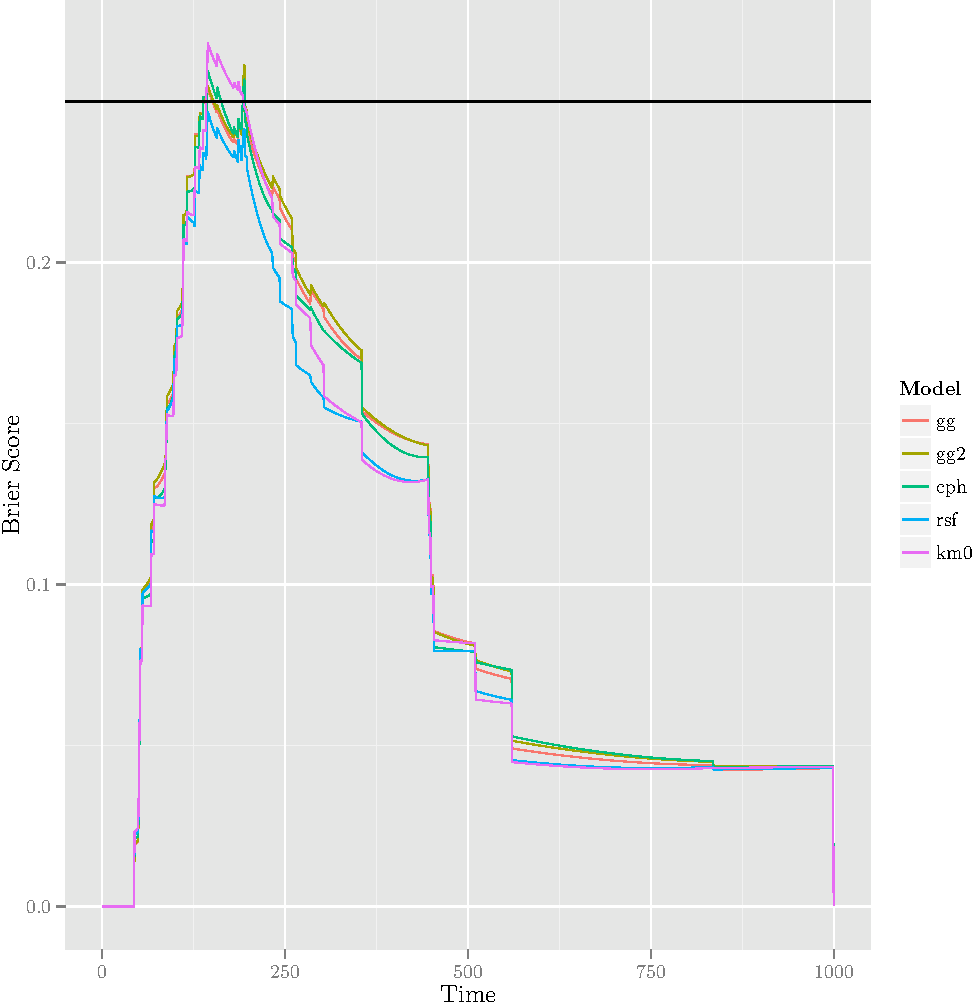
\includegraphics[width=\maxwidth]{figure/05-model-selection-bs-paths-1} 

}


\begin{kframe}\begin{alltt}
\hlstd{temp} \hlkwb{=} \hlkwd{melt}\hlstd{(}\hlkwd{aaply}\hlstd{(bsc_boots,} \hlnum{2}\hlopt{:}\hlnum{3}\hlstd{, quantile,} \hlkwc{probs} \hlstd{=} \hlkwd{c}\hlstd{(}\hlnum{0.05}\hlstd{,} \hlnum{0.5}\hlstd{,} \hlnum{0.95}\hlstd{)))}
\hlkwd{colnames}\hlstd{(temp)} \hlkwb{=} \hlkwd{c}\hlstd{(}\hlstr{"Model"}\hlstd{,} \hlstr{"Time"}\hlstd{,} \hlstr{"Quantile"}\hlstd{,} \hlstr{"Value"}\hlstd{)}
\hlstd{temp}\hlopt{$}\hlstd{Quantile} \hlkwb{=} \hlkwd{paste}\hlstd{(}\hlstr{"Q"}\hlstd{,} \hlkwd{gsub}\hlstd{(}\hlstr{"%"}\hlstd{,} \hlstr{""}\hlstd{, temp}\hlopt{$}\hlstd{Quantile),} \hlkwc{sep} \hlstd{=} \hlstr{""}\hlstd{)}
\hlstd{temp} \hlkwb{=} \hlkwd{dcast}\hlstd{(temp, Model} \hlopt{+} \hlstd{Time} \hlopt{~} \hlstd{Quantile,} \hlkwc{value.var} \hlstd{=} \hlstr{"Value"}\hlstd{)}
\hlkwd{ggplot}\hlstd{(temp,} \hlkwd{aes}\hlstd{(}\hlkwc{x} \hlstd{= Time,} \hlkwc{y} \hlstd{= Q50,} \hlkwc{ymin} \hlstd{= Q5,} \hlkwc{ymax} \hlstd{= Q95,} \hlkwc{colour} \hlstd{= Model,} \hlkwc{fill} \hlstd{= Model))} \hlopt{+} \hlkwd{geom_line}\hlstd{()} \hlopt{+} \hlkwd{geom_ribbon}\hlstd{(}\hlkwc{alpha} \hlstd{=} \hlnum{0.2}\hlstd{,} \hlkwc{colour} \hlstd{=} \hlnum{NA}\hlstd{)} \hlopt{+} \hlkwd{ylab}\hlstd{(}\hlstr{"Brier Score, 90\textbackslash{}\textbackslash{}% BI"}\hlstd{)} \hlopt{+} \hlkwd{geom_hline}\hlstd{(}\hlkwc{yintercept} \hlstd{=} \hlnum{0.25}\hlstd{)}
\end{alltt}
\end{kframe}

{\centering 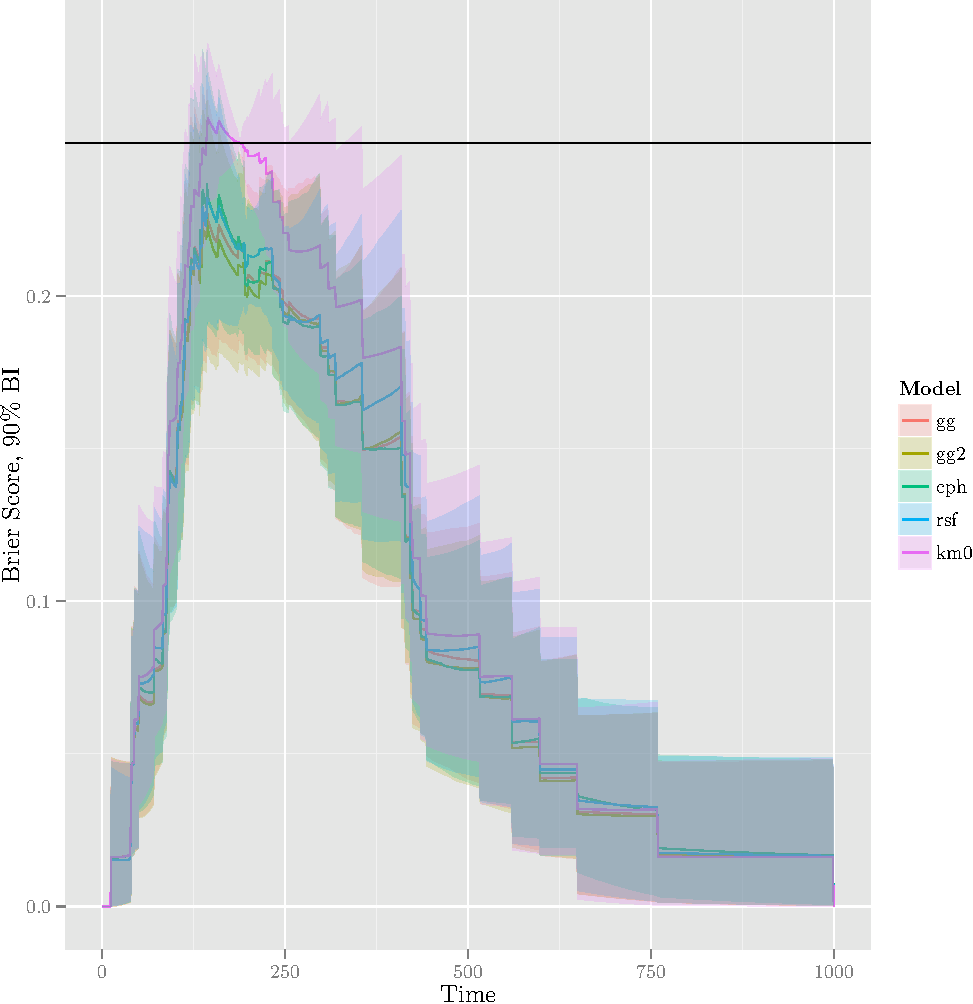
\includegraphics[width=\maxwidth]{figure/05-model-selection-bs-paths-2} 

}


\begin{kframe}\begin{alltt}
\hlstd{bsc_boots_diff} \hlkwb{=} \hlkwd{aaply}\hlstd{(bsc_boots,} \hlnum{2}\hlstd{,} \hlkwa{function}\hlstd{(}\hlkwc{x}\hlstd{) x} \hlopt{-} \hlstd{bsc_boots[,}\hlnum{5}\hlstd{,])[}\hlnum{1}\hlopt{:}\hlnum{4}\hlstd{,,]}
\hlstd{temp} \hlkwb{=} \hlkwd{melt}\hlstd{(}\hlkwd{aaply}\hlstd{(bsc_boots_diff,} \hlkwd{c}\hlstd{(}\hlnum{1}\hlstd{,}\hlnum{3}\hlstd{), quantile,} \hlkwc{probs} \hlstd{=} \hlkwd{c}\hlstd{(}\hlnum{0.05}\hlstd{,} \hlnum{0.5}\hlstd{,} \hlnum{0.95}\hlstd{)))}
\hlkwd{colnames}\hlstd{(temp)} \hlkwb{=} \hlkwd{c}\hlstd{(}\hlstr{"Model"}\hlstd{,} \hlstr{"Time"}\hlstd{,} \hlstr{"Quantile"}\hlstd{,} \hlstr{"Value"}\hlstd{)}
\hlstd{temp}\hlopt{$}\hlstd{Quantile} \hlkwb{=} \hlkwd{paste}\hlstd{(}\hlstr{"Q"}\hlstd{,} \hlkwd{gsub}\hlstd{(}\hlstr{"%"}\hlstd{,} \hlstr{""}\hlstd{, temp}\hlopt{$}\hlstd{Quantile),} \hlkwc{sep} \hlstd{=} \hlstr{""}\hlstd{)}
\hlstd{temp} \hlkwb{=} \hlkwd{dcast}\hlstd{(temp, Model} \hlopt{+} \hlstd{Time} \hlopt{~} \hlstd{Quantile,} \hlkwc{value.var} \hlstd{=} \hlstr{"Value"}\hlstd{)}
\hlkwd{ggplot}\hlstd{(temp,} \hlkwd{aes}\hlstd{(}\hlkwc{x} \hlstd{= Time,} \hlkwc{y} \hlstd{= Q50,} \hlkwc{ymin} \hlstd{= Q5,} \hlkwc{ymax} \hlstd{= Q95,} \hlkwc{colour} \hlstd{= Model,} \hlkwc{fill} \hlstd{= Model))} \hlopt{+} \hlkwd{geom_line}\hlstd{()} \hlopt{+} \hlkwd{geom_ribbon}\hlstd{(}\hlkwc{alpha} \hlstd{=} \hlnum{0.2}\hlstd{,} \hlkwc{colour} \hlstd{=} \hlnum{NA}\hlstd{)} \hlopt{+} \hlkwd{ylab}\hlstd{(}\hlstr{"Brier Score: Improvement over KM0. BS median, 90\textbackslash{}\textbackslash{}% BI"}\hlstd{)} \hlopt{+} \hlkwd{geom_hline}\hlstd{(}\hlkwc{yintercept} \hlstd{=} \hlnum{0}\hlstd{)}
\end{alltt}
\end{kframe}

{\centering 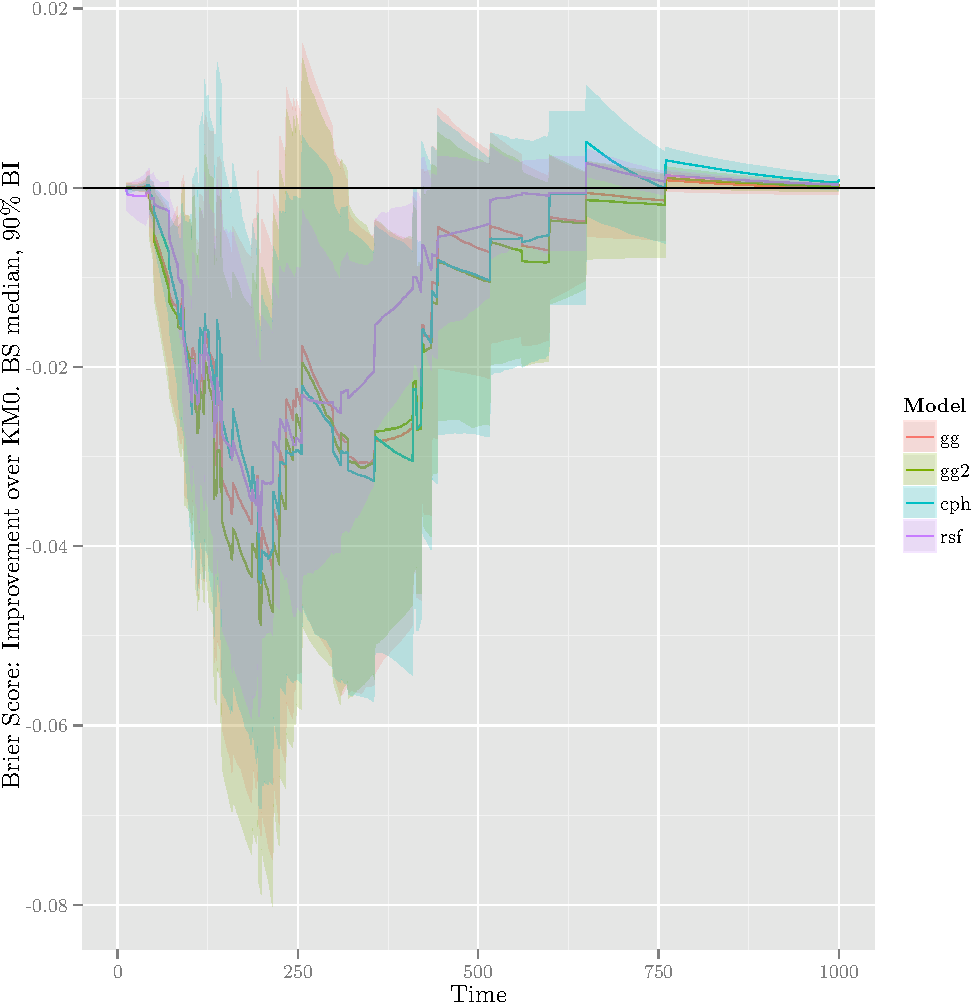
\includegraphics[width=\maxwidth]{figure/05-model-selection-bs-paths-3} 

}


\begin{kframe}\begin{alltt}
\hlkwd{ggplot}\hlstd{(temp,} \hlkwd{aes}\hlstd{(}\hlkwc{x} \hlstd{= Time,} \hlkwc{y} \hlstd{= Q50,} \hlkwc{ymin} \hlstd{= Q5,} \hlkwc{ymax} \hlstd{= Q95,} \hlkwc{colour} \hlstd{= Model,} \hlkwc{fill} \hlstd{= Model))} \hlopt{+} \hlkwd{geom_line}\hlstd{()} \hlopt{+} \hlkwd{geom_ribbon}\hlstd{(}\hlkwc{alpha} \hlstd{=} \hlnum{0.2}\hlstd{,} \hlkwc{colour} \hlstd{=} \hlnum{NA}\hlstd{)} \hlopt{+} \hlkwd{xlim}\hlstd{(}\hlnum{0}\hlstd{,} \hlnum{700}\hlstd{)} \hlopt{+} \hlkwd{ylab}\hlstd{(}\hlstr{"Brier Score: Improvement over KM0. BS median, 90\textbackslash{}\textbackslash{}% BI"}\hlstd{)} \hlopt{+} \hlkwd{geom_hline}\hlstd{(}\hlkwc{yintercept} \hlstd{=} \hlnum{0}\hlstd{)}
\end{alltt}


{\ttfamily\noindent\color{warningcolor}{\#\# Warning: Removed 1200 rows containing missing values (geom\_path).}}\end{kframe}

{\centering 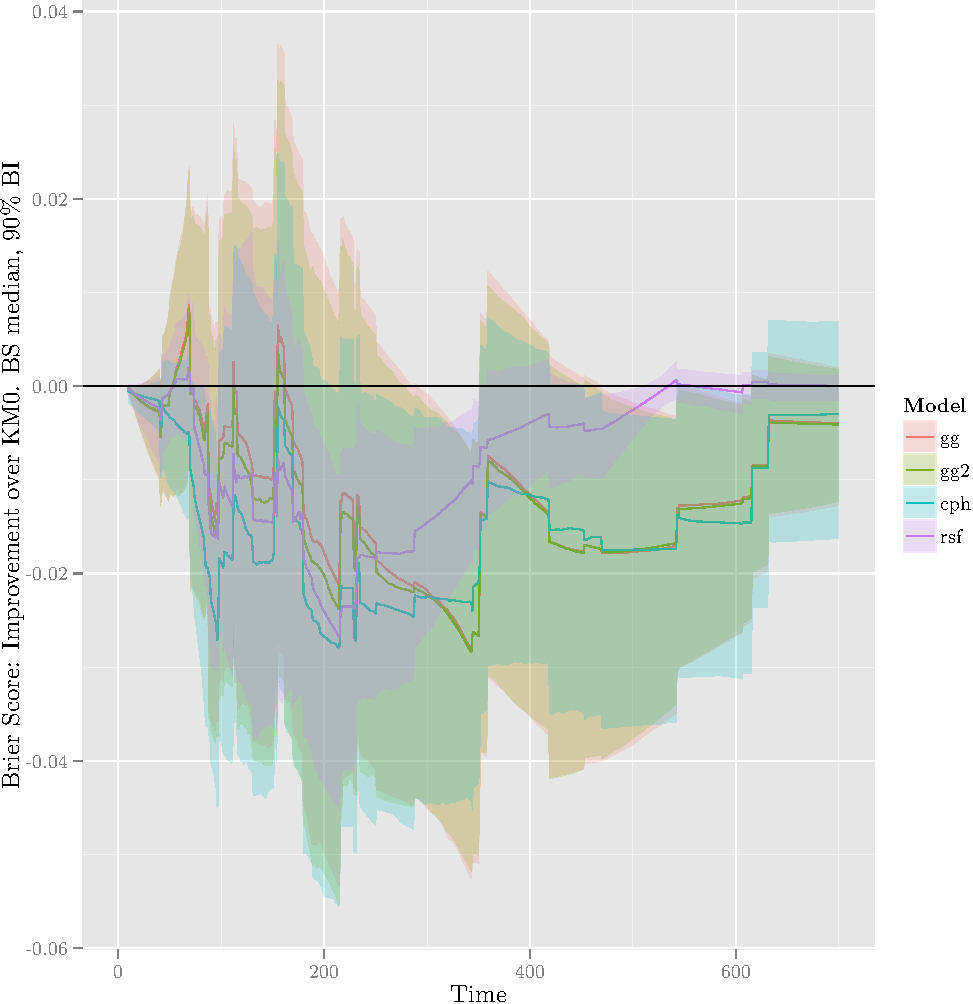
\includegraphics[width=\maxwidth]{figure/05-model-selection-bs-paths-4} 

}


\begin{kframe}\begin{alltt}
\hlkwd{ggplot}\hlstd{(temp,} \hlkwd{aes}\hlstd{(}\hlkwc{x} \hlstd{= Time,} \hlkwc{y} \hlstd{= Q50,} \hlkwc{colour} \hlstd{= Model))} \hlopt{+} \hlkwd{geom_line}\hlstd{()} \hlopt{+} \hlkwd{ylab}\hlstd{(}\hlstr{"Brier Score: Improvement over KM0, BS median"}\hlstd{)} \hlopt{+} \hlkwd{geom_hline}\hlstd{(}\hlkwc{yintercept} \hlstd{=} \hlnum{0}\hlstd{)}
\end{alltt}
\end{kframe}

{\centering 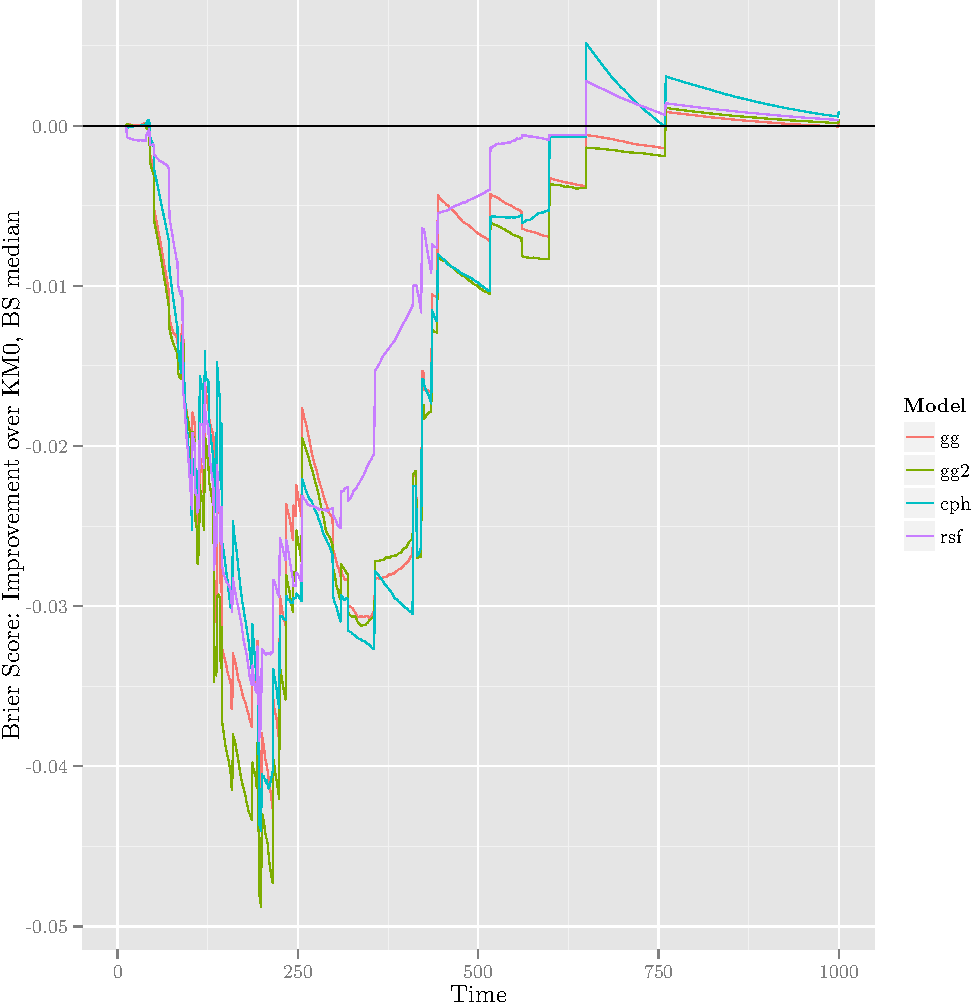
\includegraphics[width=\maxwidth]{figure/05-model-selection-bs-paths-5} 

}


\begin{kframe}\begin{alltt}
\hlkwd{ggplot}\hlstd{(temp,} \hlkwd{aes}\hlstd{(}\hlkwc{x} \hlstd{= Time,} \hlkwc{y} \hlstd{= Q50,} \hlkwc{colour} \hlstd{= Model))} \hlopt{+} \hlkwd{geom_line}\hlstd{()} \hlopt{+} \hlkwd{ylab}\hlstd{(}\hlstr{"Brier Score: Improvement over KM0, BS median"}\hlstd{)} \hlopt{+} \hlkwd{xlim}\hlstd{(}\hlnum{0}\hlstd{,} \hlnum{700}\hlstd{)} \hlopt{+} \hlkwd{geom_hline}\hlstd{(}\hlkwc{yintercept} \hlstd{=} \hlnum{0}\hlstd{)}
\end{alltt}


{\ttfamily\noindent\color{warningcolor}{\#\# Warning: Removed 1200 rows containing missing values (geom\_path).}}\end{kframe}

{\centering 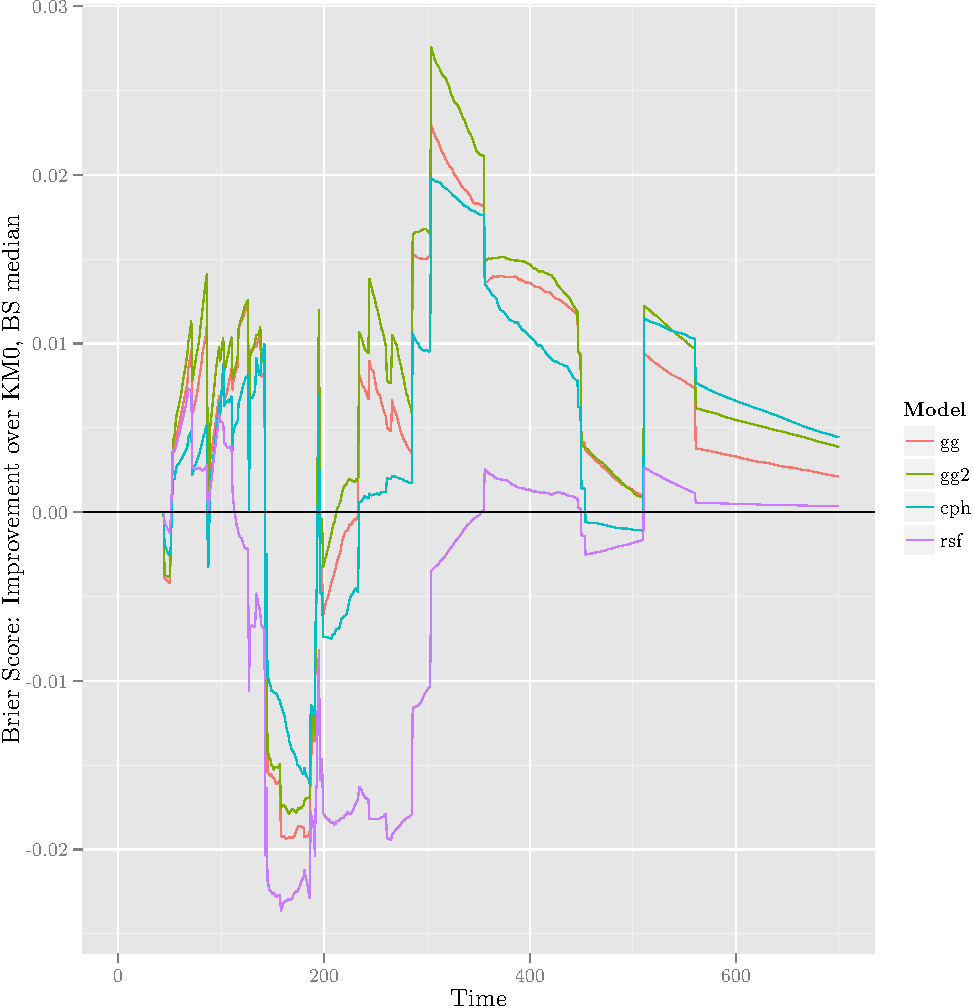
\includegraphics[width=\maxwidth]{figure/05-model-selection-bs-paths-6} 

}



\end{knitrout}

IBS comparisons.
\begin{knitrout}
\definecolor{shadecolor}{rgb}{0.969, 0.969, 0.969}\color{fgcolor}\begin{kframe}
\begin{alltt}
\hlkwd{set.seed}\hlstd{(}\hlnum{20150111}\hlstd{)}
\hlstd{ibsc_boots} \hlkwb{=} \hlkwd{t}\hlstd{(}\hlkwd{sapply}\hlstd{(}\hlnum{1}\hlopt{:}\hlnum{5e2}\hlstd{,} \hlkwa{function}\hlstd{(}\hlkwc{i}\hlstd{) \{}
        \hlkwa{if} \hlstd{(i} \hlopt \hlnum{5e1} \hlopt{==} \hlnum{0}\hlstd{)      \{} \hlkwd{message}\hlstd{(i) \}}
        \hlstd{boot_samp} \hlkwb{=} \hlkwd{sample.int}\hlstd{(}\hlkwd{nrow}\hlstd{(data.val),} \hlkwc{replace} \hlstd{=} \hlnum{TRUE}\hlstd{)}
        \hlstd{gg} \hlkwb{=} \hlkwd{calcIBS}\hlstd{(}\hlkwd{Surv}\hlstd{(data.val}\hlopt{$}\hlstd{Time, data.val}\hlopt{$}\hlstd{DSD)[boot_samp,], ibs_preds_gg[boot_samp,], ibs_times,} \hlkwd{max}\hlstd{(data.val}\hlopt{$}\hlstd{Time[boot_samp]))}\hlopt{$}\hlstd{ibs}
        \hlstd{gg2} \hlkwb{=} \hlkwd{calcIBS}\hlstd{(}\hlkwd{Surv}\hlstd{(data.val}\hlopt{$}\hlstd{Time, data.val}\hlopt{$}\hlstd{DSD)[boot_samp,], ibs_preds_gg2[boot_samp,], ibs_times,} \hlkwd{max}\hlstd{(data.val}\hlopt{$}\hlstd{Time[boot_samp]))}\hlopt{$}\hlstd{ibs}
        \hlstd{cph} \hlkwb{=} \hlkwd{calcIBS}\hlstd{(}\hlkwd{Surv}\hlstd{(data.val}\hlopt{$}\hlstd{Time, data.val}\hlopt{$}\hlstd{DSD)[boot_samp,], ibs_preds_cph[boot_samp,], ibs_times,} \hlkwd{max}\hlstd{(data.val}\hlopt{$}\hlstd{Time[boot_samp]))}\hlopt{$}\hlstd{ibs}
        \hlstd{rsf} \hlkwb{=} \hlkwd{calcIBS}\hlstd{(}\hlkwd{Surv}\hlstd{(data.val}\hlopt{$}\hlstd{Time, data.val}\hlopt{$}\hlstd{DSD)[boot_samp,], ibs_preds_rsf[boot_samp,], ibs_times,} \hlkwd{max}\hlstd{(data.val}\hlopt{$}\hlstd{Time[boot_samp]))}\hlopt{$}\hlstd{ibs}
        \hlstd{km0} \hlkwb{=} \hlkwd{calcIBS}\hlstd{(}\hlkwd{Surv}\hlstd{(data.val}\hlopt{$}\hlstd{Time, data.val}\hlopt{$}\hlstd{DSD)[boot_samp,], ibs_preds_km0[boot_samp,], ibs_times,} \hlkwd{max}\hlstd{(data.val}\hlopt{$}\hlstd{Time[boot_samp]))}\hlopt{$}\hlstd{ibs}
        \hlkwd{c}\hlstd{(gg, gg2, cph, rsf, km0)}
\hlstd{\}))}
\end{alltt}


{\ttfamily\noindent\itshape\color{messagecolor}{\#\# 50\\\#\# 100\\\#\# 150\\\#\# 200\\\#\# 250\\\#\# 300\\\#\# 350\\\#\# 400\\\#\# 450\\\#\# 500}}\begin{alltt}
\hlkwd{colnames}\hlstd{(ibsc_boots)} \hlkwb{=} \hlkwd{c}\hlstd{(}\hlstr{"gg"}\hlstd{,} \hlstr{"gg2"}\hlstd{,} \hlstr{"cph"}\hlstd{,} \hlstr{"rsf"}\hlstd{,} \hlstr{"km0"}\hlstd{)}
\end{alltt}
\end{kframe}
\end{knitrout}

\begin{knitrout}
\definecolor{shadecolor}{rgb}{0.969, 0.969, 0.969}\color{fgcolor}\begin{kframe}
\begin{alltt}
\hlkwd{calcIBS}\hlstd{(}\hlkwd{Surv}\hlstd{(data.val}\hlopt{$}\hlstd{Time, data.val}\hlopt{$}\hlstd{DSD), ibs_preds_gg, ibs_times,} \hlkwd{max}\hlstd{(data.val}\hlopt{$}\hlstd{Time))}\hlopt{$}\hlstd{ibs}
\end{alltt}
\begin{verbatim}
## [1] 184.8
\end{verbatim}
\begin{alltt}
\hlkwd{calcIBS}\hlstd{(}\hlkwd{Surv}\hlstd{(data.val}\hlopt{$}\hlstd{Time, data.val}\hlopt{$}\hlstd{DSD), ibs_preds_gg2, ibs_times,} \hlkwd{max}\hlstd{(data.val}\hlopt{$}\hlstd{Time))}\hlopt{$}\hlstd{ibs}
\end{alltt}
\begin{verbatim}
## [1] 187.6
\end{verbatim}
\begin{alltt}
\hlkwd{calcIBS}\hlstd{(}\hlkwd{Surv}\hlstd{(data.val}\hlopt{$}\hlstd{Time, data.val}\hlopt{$}\hlstd{DSD), ibs_preds_cph, ibs_times,} \hlkwd{max}\hlstd{(data.val}\hlopt{$}\hlstd{Time))}\hlopt{$}\hlstd{ibs}
\end{alltt}
\begin{verbatim}
## [1] 184.6
\end{verbatim}
\begin{alltt}
\hlkwd{calcIBS}\hlstd{(}\hlkwd{Surv}\hlstd{(data.val}\hlopt{$}\hlstd{Time, data.val}\hlopt{$}\hlstd{DSD), ibs_preds_rsf, ibs_times,} \hlkwd{max}\hlstd{(data.val}\hlopt{$}\hlstd{Time))}\hlopt{$}\hlstd{ibs}
\end{alltt}
\begin{verbatim}
## [1] 171.6
\end{verbatim}
\begin{alltt}
\hlkwd{calcIBS}\hlstd{(}\hlkwd{Surv}\hlstd{(data.val}\hlopt{$}\hlstd{Time, data.val}\hlopt{$}\hlstd{DSD), ibs_preds_km0, ibs_times,} \hlkwd{max}\hlstd{(data.val}\hlopt{$}\hlstd{Time))}\hlopt{$}\hlstd{ibs}
\end{alltt}
\begin{verbatim}
## [1] 176.5
\end{verbatim}
\begin{alltt}
\hlkwd{boxplot}\hlstd{(ibsc_boots,} \hlkwc{main} \hlstd{=} \hlstr{"IBS BS Distribution"}\hlstd{,} \hlkwc{ylab} \hlstd{=} \hlstr{"IBS"}\hlstd{)}
\end{alltt}
\end{kframe}

{\centering 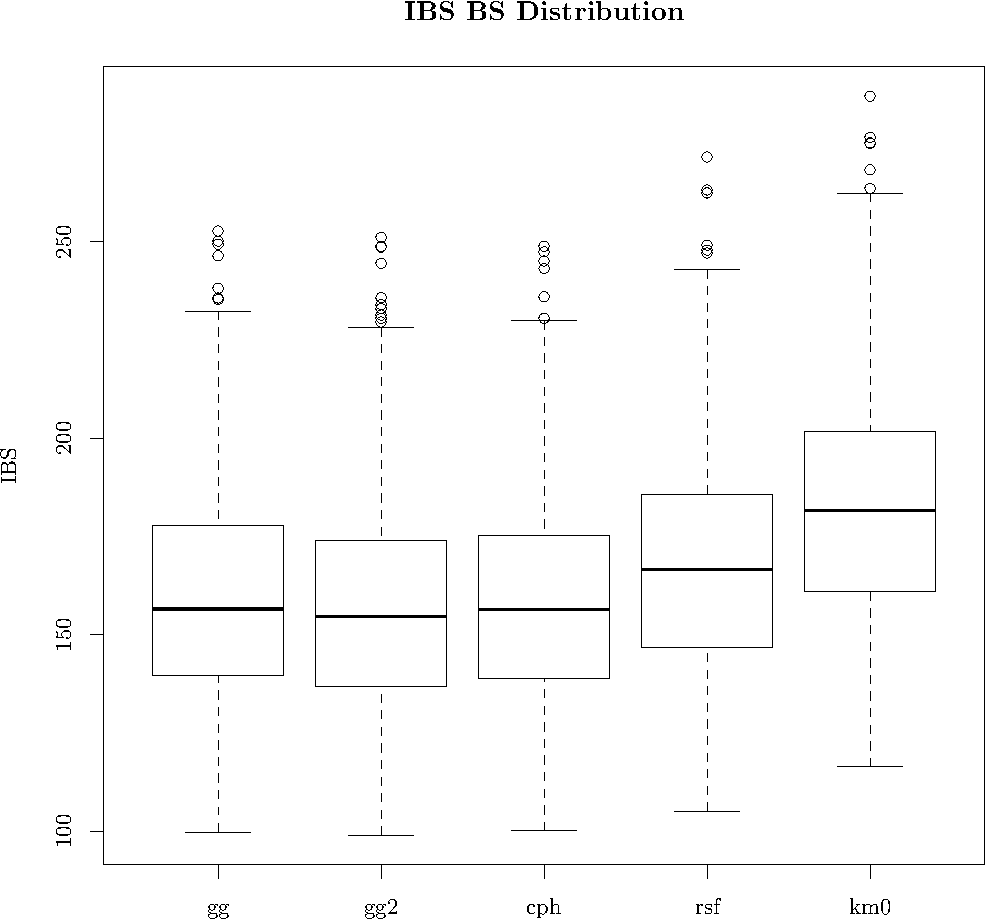
\includegraphics[width=\maxwidth]{figure/05-model-selection-ibs-1} 

}


\begin{kframe}\begin{alltt}
\hlkwd{plot}\hlstd{(}\hlkwd{density}\hlstd{(ibsc_boots[,}\hlnum{1}\hlstd{]),} \hlkwc{col} \hlstd{=} \hlstr{"blue"}\hlstd{,} \hlkwc{lwd} \hlstd{=} \hlnum{2}\hlstd{,} \hlkwc{main} \hlstd{=} \hlstr{"IBS BS Distribution"}\hlstd{,} \hlkwc{xlab} \hlstd{=} \hlstr{"IBS"}\hlstd{)}
\hlkwd{lines}\hlstd{(}\hlkwd{density}\hlstd{(ibsc_boots[,}\hlnum{2}\hlstd{]),} \hlkwc{col} \hlstd{=} \hlstr{"red"}\hlstd{,} \hlkwc{lwd} \hlstd{=} \hlnum{2}\hlstd{)}
\hlkwd{lines}\hlstd{(}\hlkwd{density}\hlstd{(ibsc_boots[,}\hlnum{3}\hlstd{]),} \hlkwc{col} \hlstd{=} \hlstr{"green"}\hlstd{,} \hlkwc{lwd} \hlstd{=} \hlnum{2}\hlstd{)}
\hlkwd{lines}\hlstd{(}\hlkwd{density}\hlstd{(ibsc_boots[,}\hlnum{4}\hlstd{]),} \hlkwc{col} \hlstd{=} \hlstr{"purple"}\hlstd{,} \hlkwc{lwd} \hlstd{=} \hlnum{2}\hlstd{)}
\hlkwd{lines}\hlstd{(}\hlkwd{density}\hlstd{(ibsc_boots[,}\hlnum{5}\hlstd{]),} \hlkwc{col} \hlstd{=} \hlstr{"black"}\hlstd{,} \hlkwc{lwd} \hlstd{=} \hlnum{2}\hlstd{)}
\hlkwd{abline}\hlstd{(}\hlkwc{v} \hlstd{=} \hlkwd{calcIBS}\hlstd{(}\hlkwd{Surv}\hlstd{(data.val}\hlopt{$}\hlstd{Time, data.val}\hlopt{$}\hlstd{DSD), ibs_preds_gg, ibs_times,} \hlkwd{max}\hlstd{(data.val}\hlopt{$}\hlstd{Time))}\hlopt{$}\hlstd{ibs,} \hlkwc{col} \hlstd{=} \hlstr{"blue"}\hlstd{,} \hlkwc{lwd} \hlstd{=} \hlnum{1}\hlstd{)}
\hlkwd{abline}\hlstd{(}\hlkwc{v} \hlstd{=} \hlkwd{calcIBS}\hlstd{(}\hlkwd{Surv}\hlstd{(data.val}\hlopt{$}\hlstd{Time, data.val}\hlopt{$}\hlstd{DSD), ibs_preds_gg2, ibs_times,} \hlkwd{max}\hlstd{(data.val}\hlopt{$}\hlstd{Time))}\hlopt{$}\hlstd{ibs,} \hlkwc{col} \hlstd{=} \hlstr{"red"}\hlstd{,} \hlkwc{lwd} \hlstd{=} \hlnum{1}\hlstd{)}
\hlkwd{abline}\hlstd{(}\hlkwc{v} \hlstd{=} \hlkwd{calcIBS}\hlstd{(}\hlkwd{Surv}\hlstd{(data.val}\hlopt{$}\hlstd{Time, data.val}\hlopt{$}\hlstd{DSD), ibs_preds_cph, ibs_times,} \hlkwd{max}\hlstd{(data.val}\hlopt{$}\hlstd{Time))}\hlopt{$}\hlstd{ibs,} \hlkwc{col} \hlstd{=} \hlstr{"green"}\hlstd{,} \hlkwc{lwd} \hlstd{=} \hlnum{1}\hlstd{)}
\hlkwd{abline}\hlstd{(}\hlkwc{v} \hlstd{=} \hlkwd{calcIBS}\hlstd{(}\hlkwd{Surv}\hlstd{(data.val}\hlopt{$}\hlstd{Time, data.val}\hlopt{$}\hlstd{DSD), ibs_preds_rsf, ibs_times,} \hlkwd{max}\hlstd{(data.val}\hlopt{$}\hlstd{Time))}\hlopt{$}\hlstd{ibs,} \hlkwc{col} \hlstd{=} \hlstr{"purple"}\hlstd{,} \hlkwc{lwd} \hlstd{=} \hlnum{1}\hlstd{)}
\hlkwd{abline}\hlstd{(}\hlkwc{v} \hlstd{=} \hlkwd{calcIBS}\hlstd{(}\hlkwd{Surv}\hlstd{(data.val}\hlopt{$}\hlstd{Time, data.val}\hlopt{$}\hlstd{DSD), ibs_preds_km0, ibs_times,} \hlkwd{max}\hlstd{(data.val}\hlopt{$}\hlstd{Time))}\hlopt{$}\hlstd{ibs,} \hlkwc{col} \hlstd{=} \hlstr{"black"}\hlstd{,} \hlkwc{lwd} \hlstd{=} \hlnum{1}\hlstd{)}
\hlkwd{legend}\hlstd{(}\hlstr{"topright"}\hlstd{,} \hlkwc{legend} \hlstd{=} \hlkwd{c}\hlstd{(}\hlstr{"gg"}\hlstd{,} \hlstr{"gg2"}\hlstd{,} \hlstr{"cph"}\hlstd{,} \hlstr{"rsf"}\hlstd{,} \hlstr{"km0"}\hlstd{),} \hlkwc{col} \hlstd{=} \hlkwd{c}\hlstd{(}\hlstr{"blue"}\hlstd{,} \hlstr{"red"}\hlstd{,} \hlstr{"green"}\hlstd{,} \hlstr{"purple"}\hlstd{,} \hlstr{"black"}\hlstd{),} \hlkwc{lty} \hlstd{=} \hlstr{"solid"}\hlstd{,} \hlkwc{inset} \hlstd{=} \hlnum{0.05}\hlstd{)}
\end{alltt}
\end{kframe}

{\centering 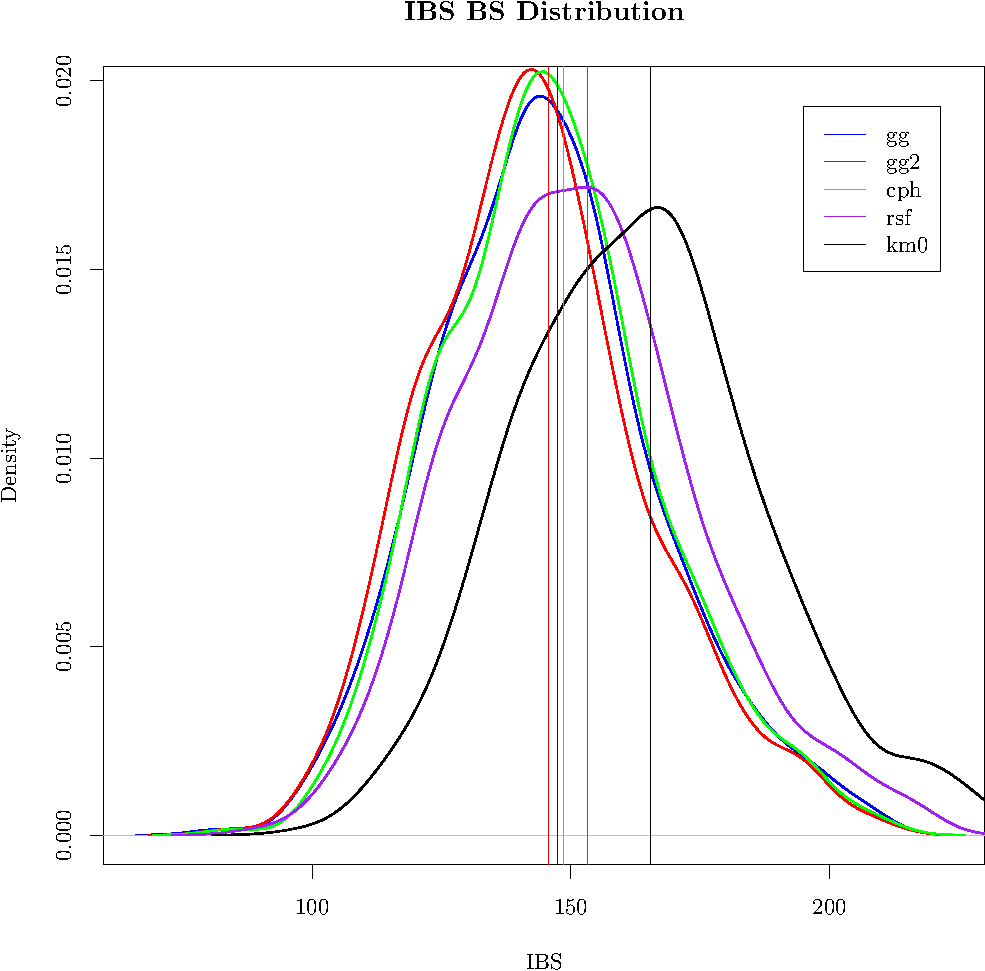
\includegraphics[width=\maxwidth]{figure/05-model-selection-ibs-2} 

}


\begin{kframe}\begin{alltt}
\hlkwd{plot}\hlstd{(}\hlkwd{density}\hlstd{(ibsc_boots[,}\hlnum{5}\hlstd{]} \hlopt{-} \hlstd{ibsc_boots[,}\hlnum{1}\hlstd{]),} \hlkwc{col} \hlstd{=} \hlstr{"blue"}\hlstd{,} \hlkwc{lwd} \hlstd{=} \hlnum{2}\hlstd{,} \hlkwc{main} \hlstd{=} \hlstr{"IBS\textbackslash{}\textbackslash{}_KM0 - IBS\textbackslash{}\textbackslash{}_x BS Distribution"}\hlstd{,} \hlkwc{xlab} \hlstd{=} \hlstr{"IBS"}\hlstd{,} \hlkwc{ylim} \hlstd{=} \hlkwd{c}\hlstd{(}\hlnum{0}\hlstd{,} \hlnum{0.1}\hlstd{))}
\hlkwd{lines}\hlstd{(}\hlkwd{density}\hlstd{(ibsc_boots[,}\hlnum{5}\hlstd{]} \hlopt{-} \hlstd{ibsc_boots[,}\hlnum{2}\hlstd{]),} \hlkwc{col} \hlstd{=} \hlstr{"red"}\hlstd{,} \hlkwc{lwd} \hlstd{=} \hlnum{2}\hlstd{)}
\hlkwd{lines}\hlstd{(}\hlkwd{density}\hlstd{(ibsc_boots[,}\hlnum{5}\hlstd{]} \hlopt{-} \hlstd{ibsc_boots[,}\hlnum{3}\hlstd{]),} \hlkwc{col} \hlstd{=} \hlstr{"green"}\hlstd{,} \hlkwc{lwd} \hlstd{=} \hlnum{2}\hlstd{)}
\hlkwd{lines}\hlstd{(}\hlkwd{density}\hlstd{(ibsc_boots[,}\hlnum{5}\hlstd{]} \hlopt{-} \hlstd{ibsc_boots[,}\hlnum{4}\hlstd{]),} \hlkwc{col} \hlstd{=} \hlstr{"purple"}\hlstd{,} \hlkwc{lwd} \hlstd{=} \hlnum{2}\hlstd{)}
\hlkwd{abline}\hlstd{(}\hlkwc{v} \hlstd{= (}\hlkwd{calcIBS}\hlstd{(}\hlkwd{Surv}\hlstd{(data.val}\hlopt{$}\hlstd{Time, data.val}\hlopt{$}\hlstd{DSD), ibs_preds_km0, ibs_times,} \hlkwd{max}\hlstd{(data.val}\hlopt{$}\hlstd{Time))}\hlopt{$}\hlstd{ibs} \hlopt{-} \hlkwd{calcIBS}\hlstd{(}\hlkwd{Surv}\hlstd{(data.val}\hlopt{$}\hlstd{Time, data.val}\hlopt{$}\hlstd{DSD), ibs_preds_gg, ibs_times,} \hlkwd{max}\hlstd{(data.val}\hlopt{$}\hlstd{Time))}\hlopt{$}\hlstd{ibs),} \hlkwc{col} \hlstd{=} \hlstr{"blue"}\hlstd{,} \hlkwc{lwd} \hlstd{=} \hlnum{1}\hlstd{)}
\hlkwd{abline}\hlstd{(}\hlkwc{v} \hlstd{= (}\hlkwd{calcIBS}\hlstd{(}\hlkwd{Surv}\hlstd{(data.val}\hlopt{$}\hlstd{Time, data.val}\hlopt{$}\hlstd{DSD), ibs_preds_km0, ibs_times,} \hlkwd{max}\hlstd{(data.val}\hlopt{$}\hlstd{Time))}\hlopt{$}\hlstd{ibs} \hlopt{-} \hlkwd{calcIBS}\hlstd{(}\hlkwd{Surv}\hlstd{(data.val}\hlopt{$}\hlstd{Time, data.val}\hlopt{$}\hlstd{DSD), ibs_preds_gg2, ibs_times,} \hlkwd{max}\hlstd{(data.val}\hlopt{$}\hlstd{Time))}\hlopt{$}\hlstd{ibs),} \hlkwc{col} \hlstd{=} \hlstr{"red"}\hlstd{,} \hlkwc{lwd} \hlstd{=} \hlnum{1}\hlstd{)}
\hlkwd{abline}\hlstd{(}\hlkwc{v} \hlstd{= (}\hlkwd{calcIBS}\hlstd{(}\hlkwd{Surv}\hlstd{(data.val}\hlopt{$}\hlstd{Time, data.val}\hlopt{$}\hlstd{DSD), ibs_preds_km0, ibs_times,} \hlkwd{max}\hlstd{(data.val}\hlopt{$}\hlstd{Time))}\hlopt{$}\hlstd{ibs} \hlopt{-} \hlkwd{calcIBS}\hlstd{(}\hlkwd{Surv}\hlstd{(data.val}\hlopt{$}\hlstd{Time, data.val}\hlopt{$}\hlstd{DSD), ibs_preds_cph, ibs_times,} \hlkwd{max}\hlstd{(data.val}\hlopt{$}\hlstd{Time))}\hlopt{$}\hlstd{ibs),} \hlkwc{col} \hlstd{=} \hlstr{"green"}\hlstd{,} \hlkwc{lwd} \hlstd{=} \hlnum{1}\hlstd{)}
\hlkwd{abline}\hlstd{(}\hlkwc{v} \hlstd{= (}\hlkwd{calcIBS}\hlstd{(}\hlkwd{Surv}\hlstd{(data.val}\hlopt{$}\hlstd{Time, data.val}\hlopt{$}\hlstd{DSD), ibs_preds_km0, ibs_times,} \hlkwd{max}\hlstd{(data.val}\hlopt{$}\hlstd{Time))}\hlopt{$}\hlstd{ibs} \hlopt{-} \hlkwd{calcIBS}\hlstd{(}\hlkwd{Surv}\hlstd{(data.val}\hlopt{$}\hlstd{Time, data.val}\hlopt{$}\hlstd{DSD), ibs_preds_rsf, ibs_times,} \hlkwd{max}\hlstd{(data.val}\hlopt{$}\hlstd{Time))}\hlopt{$}\hlstd{ibs),} \hlkwc{col} \hlstd{=} \hlstr{"purple"}\hlstd{,} \hlkwc{lwd} \hlstd{=} \hlnum{1}\hlstd{)}
\hlkwd{legend}\hlstd{(}\hlstr{"topright"}\hlstd{,} \hlkwc{legend} \hlstd{=} \hlkwd{c}\hlstd{(}\hlstr{"gg"}\hlstd{,} \hlstr{"gg2"}\hlstd{,} \hlstr{"cph"}\hlstd{,} \hlstr{"rsf"}\hlstd{),} \hlkwc{col} \hlstd{=} \hlkwd{c}\hlstd{(}\hlstr{"blue"}\hlstd{,} \hlstr{"red"}\hlstd{,} \hlstr{"green"}\hlstd{,} \hlstr{"purple"}\hlstd{),} \hlkwc{lty} \hlstd{=} \hlstr{"solid"}\hlstd{,} \hlkwc{inset} \hlstd{=} \hlnum{0.05}\hlstd{)}
\end{alltt}
\end{kframe}

{\centering 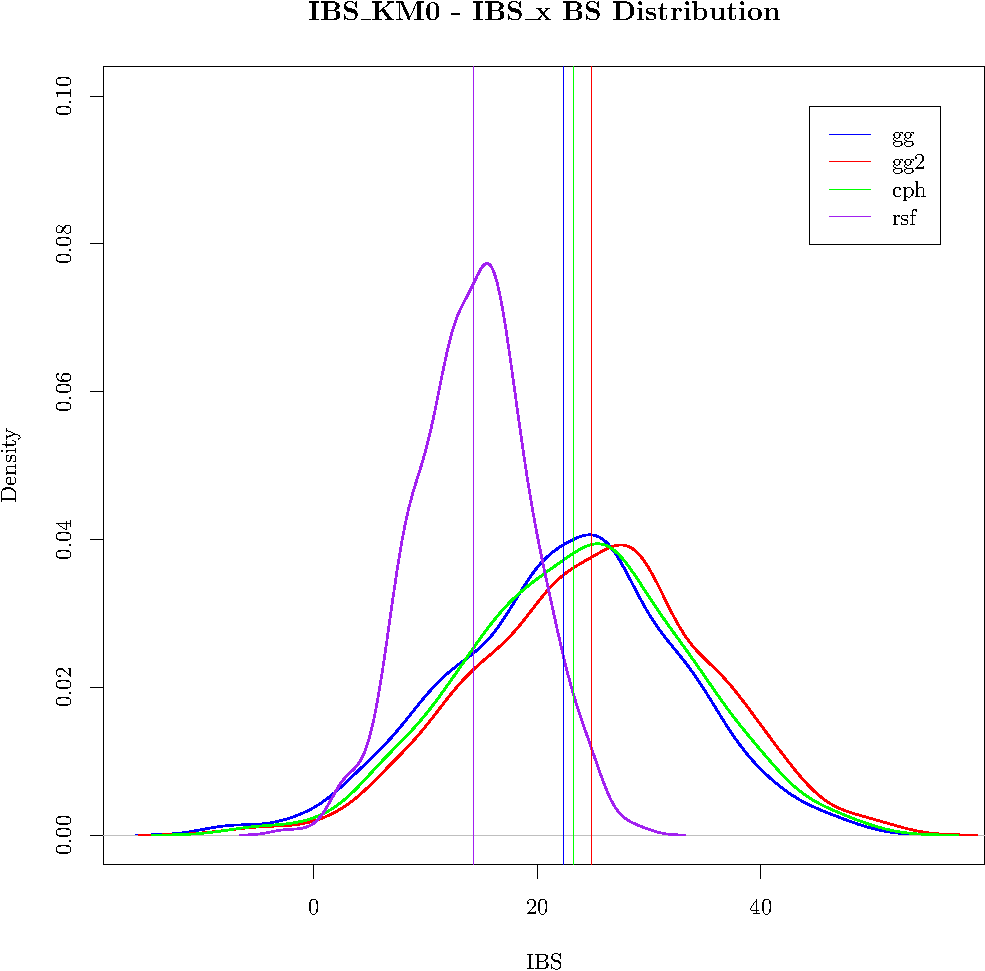
\includegraphics[width=\maxwidth]{figure/05-model-selection-ibs-3} 

}



\end{knitrout}

Do some proper BCA bootstrapping on the differences, just as a double-check test.
\begin{knitrout}
\definecolor{shadecolor}{rgb}{0.969, 0.969, 0.969}\color{fgcolor}\begin{kframe}
\begin{alltt}
\hlkwd{set.seed}\hlstd{(}\hlnum{20150111}\hlstd{)}
\hlstd{ibsc_boots2} \hlkwb{=} \hlkwd{boot}\hlstd{(data.val,} \hlkwc{statistic} \hlstd{=} \hlkwa{function}\hlstd{(}\hlkwc{d}\hlstd{,} \hlkwc{i}\hlstd{) \{}
        \hlstd{gg} \hlkwb{=} \hlkwd{calcIBS}\hlstd{(}\hlkwd{Surv}\hlstd{(d}\hlopt{$}\hlstd{Time, d}\hlopt{$}\hlstd{DSD)[i,], ibs_preds_gg[i,], ibs_times,} \hlkwd{max}\hlstd{(d}\hlopt{$}\hlstd{Time[i]))}\hlopt{$}\hlstd{ibs}
        \hlstd{gg2} \hlkwb{=} \hlkwd{calcIBS}\hlstd{(}\hlkwd{Surv}\hlstd{(d}\hlopt{$}\hlstd{Time, d}\hlopt{$}\hlstd{DSD)[i,], ibs_preds_gg2[i,], ibs_times,} \hlkwd{max}\hlstd{(d}\hlopt{$}\hlstd{Time[i]))}\hlopt{$}\hlstd{ibs}
        \hlstd{cph} \hlkwb{=} \hlkwd{calcIBS}\hlstd{(}\hlkwd{Surv}\hlstd{(d}\hlopt{$}\hlstd{Time, d}\hlopt{$}\hlstd{DSD)[i,], ibs_preds_cph[i,], ibs_times,} \hlkwd{max}\hlstd{(d}\hlopt{$}\hlstd{Time[i]))}\hlopt{$}\hlstd{ibs}
        \hlstd{rsf} \hlkwb{=} \hlkwd{calcIBS}\hlstd{(}\hlkwd{Surv}\hlstd{(d}\hlopt{$}\hlstd{Time, d}\hlopt{$}\hlstd{DSD)[i,], ibs_preds_rsf[i,], ibs_times,} \hlkwd{max}\hlstd{(d}\hlopt{$}\hlstd{Time[i]))}\hlopt{$}\hlstd{ibs}
        \hlstd{km0} \hlkwb{=} \hlkwd{calcIBS}\hlstd{(}\hlkwd{Surv}\hlstd{(d}\hlopt{$}\hlstd{Time, d}\hlopt{$}\hlstd{DSD)[i,], ibs_preds_km0[i,], ibs_times,} \hlkwd{max}\hlstd{(d}\hlopt{$}\hlstd{Time[i]))}\hlopt{$}\hlstd{ibs}
        \hlkwd{c}\hlstd{(gg} \hlopt{-} \hlstd{km0, gg2} \hlopt{-} \hlstd{km0, cph} \hlopt{-} \hlstd{km0, rsf} \hlopt{-} \hlstd{km0, gg} \hlopt{-} \hlstd{rsf, gg2} \hlopt{-} \hlstd{rsf, cph} \hlopt{-} \hlstd{rsf, gg} \hlopt{-} \hlstd{cph, gg2} \hlopt{-} \hlstd{cph, gg} \hlopt{-} \hlstd{gg2)}
\hlstd{\},} \hlkwc{R} \hlstd{=} \hlnum{500}\hlstd{)}
\hlstd{ibsc_boots2_ci} \hlkwb{=} \hlkwd{t}\hlstd{(}\hlkwd{sapply}\hlstd{(}\hlnum{1}\hlopt{:}\hlkwd{length}\hlstd{(ibsc_boots2}\hlopt{$}\hlstd{t0),} \hlkwa{function}\hlstd{(}\hlkwc{i}\hlstd{)} \hlkwd{boot.ci}\hlstd{(ibsc_boots2,} \hlkwc{index} \hlstd{= i,} \hlkwc{type} \hlstd{=} \hlstr{"bca"}\hlstd{)}\hlopt{$}\hlstd{bca))}
\hlkwd{rownames}\hlstd{(ibsc_boots2_ci)} \hlkwb{=} \hlkwd{c}\hlstd{(}\hlstr{"gg-km0"}\hlstd{,} \hlstr{"gg2-km0"}\hlstd{,} \hlstr{"cph-km0"}\hlstd{,} \hlstr{"rsf-km0"}\hlstd{,} \hlstr{"gg-rsf"}\hlstd{,} \hlstr{"gg2-rsf"}\hlstd{,} \hlstr{"cph-rsf"}\hlstd{,} \hlstr{"gg-cph"}\hlstd{,} \hlstr{"gg2-cph"}\hlstd{,} \hlstr{"gg-gg2"}\hlstd{)}
\hlkwd{colnames}\hlstd{(ibsc_boots2_ci)} \hlkwb{=} \hlkwd{c}\hlstd{(}\hlstr{"level"}\hlstd{,} \hlstr{"orderi1"}\hlstd{,} \hlstr{"orderi2"}\hlstd{,} \hlstr{"lci"}\hlstd{,} \hlstr{"uci"}\hlstd{)}
\hlstd{ibsc_boots2}
\end{alltt}
\begin{verbatim}
## 
## ORDINARY NONPARAMETRIC BOOTSTRAP
## 
## 
## Call:
## boot(data = data.val, statistic = function(d, i) {
##     gg = calcIBS(Surv(d$Time, d$DSD)[i, ], ibs_preds_gg[i, ], 
##         ibs_times, max(d$Time[i]))$ibs
##     gg2 = calcIBS(Surv(d$Time, d$DSD)[i, ], ibs_preds_gg2[i, 
##         ], ibs_times, max(d$Time[i]))$ibs
##     cph = calcIBS(Surv(d$Time, d$DSD)[i, ], ibs_preds_cph[i, 
##         ], ibs_times, max(d$Time[i]))$ibs
##     rsf = calcIBS(Surv(d$Time, d$DSD)[i, ], ibs_preds_rsf[i, 
##         ], ibs_times, max(d$Time[i]))$ibs
##     km0 = calcIBS(Surv(d$Time, d$DSD)[i, ], ibs_preds_km0[i, 
##         ], ibs_times, max(d$Time[i]))$ibs
##     c(gg - km0, gg2 - km0, cph - km0, rsf - km0, gg - rsf, gg2 - 
##         rsf, cph - rsf, gg - cph, gg2 - cph, gg - gg2)
## }, R = 500)
## 
## 
## Bootstrap Statistics :
##      original   bias    std. error
## t1*    8.3816 -0.39581      11.215
## t2*   11.1692 -0.62946      12.042
## t3*    8.1730 -0.81447      11.557
## t4*   -4.8194 -0.07519       4.942
## t5*   13.2010 -0.32062       7.411
## t6*   15.9885 -0.55427       7.973
## t7*   12.9923 -0.73928       7.861
## t8*    0.2086  0.41866       3.439
## t9*    2.9962  0.18501       3.412
## t10*  -2.7876  0.23365       2.616
\end{verbatim}
\begin{alltt}
\hlstd{ibsc_boots2_ci}
\end{alltt}
\begin{verbatim}
##         level orderi1 orderi2      lci    uci
## gg-km0   0.95   19.84   493.8 -10.8484 33.776
## gg2-km0  0.95   17.42   492.4 -11.3453 35.196
## cph-km0  0.95   21.22   494.3 -13.2424 34.133
## rsf-km0  0.95   14.58   490.2 -14.1529  4.356
## gg-rsf   0.95   26.87   496.7   2.0387 31.854
## gg2-rsf  0.95   21.71   494.9   2.2010 33.379
## cph-rsf  0.95   28.75   497.0   0.3927 34.086
## gg-cph   0.95    9.08   483.6  -5.9993  6.931
## gg2-cph  0.95   22.70   495.2  -2.2832 11.342
## gg-gg2   0.95    4.05   472.6  -9.2566  1.352
\end{verbatim}
\end{kframe}
\end{knitrout}
All models perform equivalently on the validation set.  Select the simplest: gg.


%%%%%%%%%%%%%%%%%%%%%%%%%%%%%%%%%%%%%%%%%%%%%%%%%%%%%%%%%%%%%%%%%%%%%%
% CALCULATE AND SAVE FINAL MODEL
%%%%%%%%%%%%%%%%%%%%%%%%%%%%%%%%%%%%%%%%%%%%%%%%%%%%%%%%%%%%%%%%%%%%%%
Final model fitting:
\begin{knitrout}
\definecolor{shadecolor}{rgb}{0.969, 0.969, 0.969}\color{fgcolor}\begin{kframe}
\begin{alltt}
\hlstd{data.all} \hlkwb{=} \hlkwd{rbind}\hlstd{(data[}\hlkwd{colnames}\hlstd{(data.val)], data.val)}
\hlkwd{head}\hlstd{(data.all)}
\end{alltt}
\begin{verbatim}
##           Time  DSD  SexM AgeCent LocBody SizeCent    A2   A4
## NSWPCN_4   937 TRUE  TRUE     -16   FALSE       -1 FALSE TRUE
## NSWPCN_9   587 TRUE  TRUE       5   FALSE       10 FALSE TRUE
## NSWPCN_10  177 TRUE  TRUE      -9   FALSE       10 FALSE TRUE
## NSWPCN_13  247 TRUE FALSE     -19    TRUE       20 FALSE TRUE
## NSWPCN_17  316 TRUE FALSE     -23   FALSE       -5 FALSE TRUE
## NSWPCN_20  256 TRUE FALSE      -8   FALSE        0 FALSE TRUE
\end{verbatim}
\begin{alltt}
\hlstd{fit.final.gg} \hlkwb{=} \hlkwd{flexsurvreg}\hlstd{(}\hlkwd{Surv}\hlstd{(Time, DSD)} \hlopt{~} \hlstd{SexM} \hlopt{+} \hlstd{SizeCent} \hlopt{+} \hlstd{A2} \hlopt{+} \hlstd{A4,}
        \hlkwc{anc} \hlstd{=} \hlkwd{list}\hlstd{(}
                \hlkwc{sigma} \hlstd{=} \hlopt{~} \hlstd{SexM,}
                \hlkwc{Q} \hlstd{=} \hlopt{~} \hlstd{SexM),}
        \hlkwc{data} \hlstd{= data.all,} \hlkwc{dist} \hlstd{=} \hlstr{"gengamma"}\hlstd{)}
\hlstd{fit.final.gg2} \hlkwb{=} \hlkwd{flexsurvreg}\hlstd{(}\hlkwd{Surv}\hlstd{(Time, DSD)} \hlopt{~} \hlstd{SexM} \hlopt{+} \hlstd{SizeCent} \hlopt{+} \hlstd{A2} \hlopt{+} \hlstd{A4} \hlopt{+} \hlkwd{I}\hlstd{(SexM} \hlopt{==} \hlnum{FALSE} \hlopt{&} \hlstd{A2} \hlopt{==} \hlnum{FALSE} \hlopt{&} \hlstd{A4} \hlopt{==} \hlnum{FALSE}\hlstd{),}
    \hlkwc{anc} \hlstd{=} \hlkwd{list}\hlstd{(}
        \hlkwc{sigma} \hlstd{=} \hlopt{~} \hlstd{SexM,}
        \hlkwc{Q} \hlstd{=} \hlopt{~} \hlstd{SexM),}
    \hlkwc{data} \hlstd{= data.all,} \hlkwc{dist} \hlstd{=} \hlstr{"gengamma"}\hlstd{)}
\hlstd{fit.final.cph} \hlkwb{=} \hlkwd{coxph}\hlstd{(}\hlkwd{Surv}\hlstd{(Time, DSD)} \hlopt{~} \hlkwd{strata}\hlstd{(SexM)} \hlopt{+} \hlstd{SizeCent} \hlopt{+} \hlstd{A2} \hlopt{+} \hlstd{A4,} \hlkwc{data} \hlstd{= data.all,} \hlkwc{x} \hlstd{=} \hlnum{TRUE}\hlstd{,} \hlkwc{y} \hlstd{=} \hlnum{TRUE}\hlstd{,} \hlkwc{model} \hlstd{=} \hlnum{TRUE}\hlstd{)}
\hlkwd{set.seed}\hlstd{(}\hlnum{20150111}\hlstd{)}
\hlstd{fit.final.rsf} \hlkwb{=} \hlkwd{rfsrc}\hlstd{(}\hlkwd{Surv}\hlstd{(Time, DSD)} \hlopt{~} \hlstd{SexM} \hlopt{+} \hlstd{AgeCent} \hlopt{+} \hlstd{LocBody} \hlopt{+} \hlstd{SizeCent} \hlopt{+} \hlstd{A2} \hlopt{+} \hlstd{A4,} \hlkwc{data} \hlstd{= data.all,} \hlkwc{mtry} \hlstd{=} \hlnum{1}\hlstd{,} \hlkwc{splitrule} \hlstd{=} \hlstr{"logrankscore"}\hlstd{,} \hlkwc{nsplit} \hlstd{=} \hlnum{2}\hlstd{,} \hlkwc{ntree} \hlstd{=} \hlnum{1000}\hlstd{)}
\hlstd{fit.final.km0} \hlkwb{=} \hlkwd{survfit}\hlstd{(}\hlkwd{Surv}\hlstd{(Time, DSD)} \hlopt{~} \hlnum{1}\hlstd{, data.all)}
\hlkwd{saveRDS}\hlstd{(}\hlkwd{list}\hlstd{(}\hlkwc{gg} \hlstd{= fit.final.gg,} \hlkwc{km0} \hlstd{= fit.final.km0,} \hlkwc{gg2} \hlstd{= fit.final.gg2,} \hlkwc{cph} \hlstd{= fit.final.cph,} \hlkwc{rsf} \hlstd{= fit.final.rsf,} \hlkwc{data.train} \hlstd{= data.all),} \hlkwc{file} \hlstd{=} \hlstr{"05_final_model.rds"}\hlstd{)}
\end{alltt}
\end{kframe}
\end{knitrout}

\begin{knitrout}
\definecolor{shadecolor}{rgb}{0.969, 0.969, 0.969}\color{fgcolor}\begin{kframe}
\begin{alltt}
\hlkwd{save.image}\hlstd{(}\hlstr{"05_train_NSWPCN_2.rda"}\hlstd{)}
\end{alltt}
\end{kframe}
\end{knitrout}

%%%%%%%%%%%%%%%%%%%%%%%%%%%%%%%%%%%%%%%%%%%%%%%%%%%%%%%%%%%%%%%%%%%%%%
% THE END
%%%%%%%%%%%%%%%%%%%%%%%%%%%%%%%%%%%%%%%%%%%%%%%%%%%%%%%%%%%%%%%%%%%%%%
\section{Session information}
\begin{knitrout}
\definecolor{shadecolor}{rgb}{0.969, 0.969, 0.969}\color{fgcolor}\begin{kframe}
\begin{alltt}
\hlkwd{sessionInfo}\hlstd{()}
\end{alltt}
\begin{verbatim}
## R version 3.1.1 (2014-07-10)
## Platform: x86_64-unknown-linux-gnu (64-bit)
## 
## locale:
##  [1] LC_CTYPE=en_AU.UTF-8          LC_NUMERIC=C                 
##  [3] LC_TIME=en_AU.UTF-8           LC_COLLATE=en_AU.UTF-8       
##  [5] LC_MONETARY=en_AU.UTF-8       LC_MESSAGES=en_AU.UTF-8      
##  [7] LC_PAPER=en_AU.UTF-8          LC_NAME=en_AU.UTF-8          
##  [9] LC_ADDRESS=en_AU.UTF-8        LC_TELEPHONE=en_AU.UTF-8     
## [11] LC_MEASUREMENT=en_AU.UTF-8    LC_IDENTIFICATION=en_AU.UTF-8
## 
## attached base packages:
## [1] parallel  methods   splines   stats     graphics  grDevices utils    
## [8] datasets  base     
## 
## other attached packages:
##  [1] timeROC_0.2           timereg_1.8.6         mvtnorm_1.0-1        
##  [4] pec_2.4.4             boot_1.3-13           MASS_7.3-35          
##  [7] ggplot2_1.0.0         plyr_1.8.1            reshape2_1.4         
## [10] randomForestSRC_1.5.5 flexsurv_0.5          glmulti_1.0.7        
## [13] rJava_0.9-6           survival_2.37-7       tikzDevice_0.8.1     
## [16] knitr_1.8            
## 
## loaded via a namespace (and not attached):
##  [1] codetools_0.2-9  colorspace_1.2-4 deSolve_1.11     digest_0.6.4    
##  [5] evaluate_0.5.5   filehash_2.2-2   foreach_1.4.2    formatR_1.0     
##  [9] grid_3.1.1       gtable_0.1.2     highr_0.4        iterators_1.0.7 
## [13] labeling_0.3     lava_1.3         muhaz_1.2.6      munsell_0.4.2   
## [17] prodlim_1.5.1    proto_0.3-10     Rcpp_0.11.3      scales_0.2.4    
## [21] stringr_0.6.2    tools_3.1.1
\end{verbatim}
\end{kframe}
\end{knitrout}

\end{document}



